\documentclass[12pt]{report}
\usepackage[hidelinks]{hyperref}
\setcounter{tocdepth}{3}
\usepackage[italian]{babel}
\usepackage[utf8]{inputenc}
\usepackage[a4paper, margin=2cm]{geometry}
\usepackage{nth}
\usepackage{fancyhdr}
\pagestyle{fancy}
\usepackage{titlesec}
\usepackage{amsmath}
\usepackage{amssymb}
\usepackage{graphicx}
\usepackage{csquotes}
\usepackage{hyperref}
\usepackage{float}
\usepackage{tcolorbox}
\usepackage{algorithm}
\usepackage{algpseudocode}
\tcbuselibrary{breakable}


\fancyhead[L]{Reti di Calcolatori}
\fancyhead[R]{Marco Ferrara}

\setlength{\headheight}{15pt}

\title{Reti di Calcolatori}
\author{Marco Ferrara} 

\begin{document}
	\maketitle
	\tableofcontents
	\newpage

	\chapter{Introduzione}
	Internet è una rete di calcolatori che interconnette miliardi di dispositivi di calcolo in tutto il mondo. Non molto tempo fa questi dispositivi di elaborazione erano fondamentalmente PC tradizionali, workstation Linux o server che immagazzinavano e trasmettevano informazioni quali pagine web e messaggi di posta elettronica.
	\vspace{\baselineskip}\\
	Al giorno d’oggi invece vengono sempre più spesso connesse a Internet “cose”, quali computer portatili, tablet, smartphone, TV, console di gioco, termostati, sistemi di sorveglianza, elettrodomestici, orologi, occhiali, automobili, sistemi di controllo del traffico e molte altre. In gergo, tutti questi dispositivi sono detti host (ospiti) o sistemi periferici (end system).
			
	\section{Le Reti}
	Una rete è un'interconnessione di dispositivi in grado di scambiarsi informazioni, quali sistemi terminali (end system), router, switch e modem. I sistemi terminali possono essere di due tipi: host o server. 
	\vspace{\baselineskip}\\
	Un host è una macchina in genere di proprietà degli utenti e dedicata ad eseguire applicazioni, quale un computer desktop, un portatile, un cellulare o un tablet.
	Un server è tipicamente un computer con elevate prestazioni destinato a eseguire programmi che forniscono servizio a diverse applicazioni utente come, per esempio, la posta elettronica o il Web. I server vengono gestiti dagli amministratori di sistema. Rientrano tra i server anche le periferiche di rete, come per esempio le stampanti, che vengono spesso condivise tra vari utenti. 
	\vspace{\baselineskip}\\
	I router sono dispositivi che collegano una rete ad altre reti, mentre gli switch (commutatori) collegano fra di loro più sistemi terminali a livello locale. È possibile che in una rete ci siano anche i modem, che trasformano la codifica dei dati. Tutti questi dispositivi vengono collegati utilizzando mezzi trasmissivi cablati o wireless, come cavi o onde radio, genericamente chiamati link (collegamenti).
	\vspace{\baselineskip}\\
	A seconda di dove sono collocati i nodi da collegare e della tecnologia utilizzata per farli comunicare tra loro, le reti possono distinguersi in:
	\begin{itemize}
		\item \textbf{PAN - Personal Area Network}
		\item \textbf{LAN - Local Area Network}
		\item \textbf{MAN - Metropolitan Area Network}
		\item \textbf{WAN - Wide Area Network}
	\end{itemize}

	\subsection{PAN - Personal Area Network}
	Una PAN (Personal Area Network), o rete personale, è una rete di dispositivi di comunicazione che si trova in genere entro un raggio di pochi metri. Una PAN può essere costituita da dispositivi collegati tramite cavi o wireless. Un esempio di PAN è la rete Bluetooth, che collega dispositivi come smartphone, tablet, auricolari e tastiere. Un'altra tecnologia per le PAN è la rete personale wireless (WPAN), che collega dispositivi come telefoni cellulari, palmari e computer portatili. Una WPAN utilizza la tecnologia radio a corto raggio per collegare i dispositivi.

	\subsection{LAN - Local Area Network}
	Una LAN (Local Area Network), o rete locale, è solitamente una rete privata che collega i com- puter in un singolo ufficio, un edificio o un comprensorio. Qualsiasi sistema terminale in una LAN deve avere un indirizzo che lo identifica univocamente nella rete. Un pacchetto inviato da un sistema terminale a un altro contiene entrambi gli indirizzi di mittente e destinatario.
	\vspace{\baselineskip}\\
	In passato tutti i dispositivi di una rete locale erano collegati mediante un cavo condiviso, o mezzo broadcast, per cui il pacchetto inviato da un dispositivo veniva ricevuto da tutti gli altri. Il destinatario elaborava il pacchetto, mentre gli altri lo dovevano ignorare. 
	\vspace{\baselineskip}\\
	Oggi la maggior parte delle LAN utilizza uno switch di interconnessione, al quale ogni dispositivo in rete è direttamente connesso. Lo switch è in grado di riconoscere l'indirizzo di destinazione e di inviare quindi il pacchetto al solo destinatario senza inviarlo agli altri dispositivi. Lo switch riduce il traffico nella LAN e consente a più coppie di dispositivi di comunicare contemporaneamente fra di loro, posto che non vi siano dispositivi sorgente o destinazione in comune. Quando le LAN erano isolate (situazione attualmente molto rara), avevano l'unico scopo di condividere risorse fra i sistemi terminali che ne facevano parte. Le LAN sono oggigiorno connesse fra di loro e a reti WAN, per consentire una comunicazione su vasta scala.

	\subsection{MAN - Metropolitan Area Network}
	Una MAN (Metropolitan Area Network) è una rete che copre un'area geografica più vasta di una LAN, come una città o una regione. Un esempio tipico di rete MAN è quello di una amministrazione comunale che collega in rete tutti i propri uffici dislocati in una città.

	\subsection{WAN - Wide Area Network}
	Anche una WAN è un'interconnessione di dispositivi in grado di comunicare, ma ci sono delle differenze rispetto a una LAN o una MAN. Una WAN è una rete che copre un'area geografica molto più vasta, come una città, un paese o un continente. Le WAN sono spesso costituite da collegamenti di proprietà di terzi, come le linee telefoniche, i cavi in fibra ottica o i satelliti. 
	\vspace{\baselineskip}\\
	Le WAN sono spesso utilizzate dalle aziende per collegare le loro sedi dislocate in diverse località. Le WAN sono spesso connesse fra di loro e a Internet. Le reti WAN sono spesso gestite da operatori di telecomunicazioni o da fornitori di servizi Internet (ISP). Esistono due tipi di WAN:
	\begin{itemize}
		\item \textbf{WAN punto-punto}: che collega due dispositivi di comunicazione tramite mezzo trasmissivo.
		\item \textbf{WAN a commutazione} (switched): rete con più di due punti di terminazione che viene utilizzata nelle dorsali della odierna rete globali.
	\end{itemize}

	\subsection{Internetwork}
	Al giorno d'oggi è erato vedere LAN e WAN isolate: esse sono in genere connesse fra di loro. formando una internetwork, o internet. Una internetwork è una collezione di reti interconnesse, ognuna con la propria tecnologia e amministrazione. Le reti sono collegate fra di loro mediante dispositivi di interconnessione, quali router, switch e gateway. 

	\section{Commutazione (switching)}
	In base al metodo adottato per determinare il percorso di un pacchetto da un mittente a un destinatario, le reti si distinguono in due tipi: a commutazione di circuito e a commutazione di pacchetto.

	\subsection{Commutazione di circuito}
	In una rete a commutazione di circuito (circuit-switched network) tra due dispositivi è sempre disponibile un collegamento dedicato chiamato circuito. Lo switch che collega i due dispositivi può solo attivarlo o disattivarlo. Quando il circuito è attivato, i due dispositivi possono comunicare fra di loro. Il circuito è dedicato e non può essere utilizzato da altri dispositivi. 
	\vspace{\baselineskip}\\
	Questo tipo di rete è simile a una chiamata telefonica: quando si effettua una chiamata, il sistema di commutazione crea un circuito tra il chiamante e il chiamato. Il circuito rimane attivo finché la chiamata non viene terminata. Questo tipo di rete è stato utilizzato per molto tempo nelle reti telefoniche, ma è stato in gran parte sostituito dalla commutazione di pacchetto. 
	\vspace{\baselineskip}\\
	Questo comporta che una rete a commutazione di circuito risulta efficiente solamente quando è utilizzata alla sua capacità massima. Se il traffico è inferiore alla capacità massima, il circuito rimane sottoutilizzato o inutilizzato. Inoltre, se il circuito è interrotto, la comunicazione viene interrotta.

	\subsection{Commutazione di pacchetto}
	In una rete a commutazione di pacchetto (packet-switched network)la comunicazione fra ai due lati viene effettuata trasmettendo blocchi di dati chiamati pacchetti. Invece di avere una comunicazione continua, i dati vengono inviati in pacchetti separati indipendenti. 
	\vspace{\baselineskip}\\
	Ogni pacchetto contiene sia i dati che l'indirizzo del destinatario. I pacchetti possono seguire percorsi diversi e possono arrivare a destinazione in ordine diverso rispetto a quello in cui sono stati inviati. I pacchetti possono essere persi, duplicati o consegnati in ritardo. 
	\vspace{\baselineskip}\\
	Un router in una rete a commutazione di pacchetto possiede una coda dove possono essere memorizzati i pacchetti prima di essere inoltrati. Questo tipo di rete è molto più flessibile rispetto a quella a commutazione di circuito. Se il traffico è inferiore alla capacità massima, i pacchetti possono essere inoltrati in modo efficiente. Inoltre, se un collegamento si interrompe, i pacchetti possono essere inoltrati su un percorso alternativo. La rete a commutazione di pacchetto è la base di Internet. Il problema sorge quando il traffico è troppo elevato: i pacchetti possono essere persi o ritardati, e la rete può diventare congestionata.

	\section{Internet}
	Una internet (con la i minuscola) è una collezione di reti interconnesse. Internet (con la I maiuscola) è la più grande e famosa internet del mondo. Internet è un insieme di dorsali, reti dei provider e reti private. 
	\vspace{\baselineskip}\\
	Al livello più elevato le dorsali sono reti particolarmente estese di proprietà delle compagnie telefoniche e sono interconnesse tramite sistemi di commutazione complessi, chiamati peering point. Al secondo livello ci sono le reti dei provider, più piccole delle dorsali, che utilizzano a pagamento i servizi delle dorsali e sono connesse ad esse e a volte ad altre reti di provider. Al terzo livello ci sono le reti private, ai confini di Internet, che utilizzano i servizi a pagamento dei provider per connettersi a Internet. Le dorsali e le reti dei provider sono anche chiamate collettivamente ISP (Internet Service Provider) rispettivamente Internazionali e Nazionali/Regionali.
	\vspace{\baselineskip}\\
	Internet consente a qualsiasi utente di farne parte. L'utente, tuttavia, deve essere fisicamente collegato ad un ISP, solitamente mediante una WAN punto-punto. Il collegamento che connette l'utente al primo router di internet è chiamato rete di accesso (o access link).

	\subsection{Accesso via rete telefonica}
	Oggi la maggior parte delle abitazioni e delle piccole aziende è dotata di servizi telefonici, quindi è collegata a una rete telefomca. Poiché molte reti telefoniche sono collegate a In- ternet, un'opzione per clienti residenziali e delle piccole aziende è quella di collegarsi a Internet modificando la linea telefonica fra la residenza o la sede della piccola azienda e la centrale telefonica con una WAN punto punto. Questo può avvenire in due modi.
	\begin{itemize}
		\item \textbf{Servizio dial-up}: consiste nell'inserire sulla linea telefonica un modem che converte i dati digitali (del computer) in analogici (per trasmetterli sulla linea telefonica) e viceversa. Il software installato sul computer compone il numero dell'ISP e esegue una comunicazione telefonica. Sfortunatamente il servizio dial-up è molto lento, inoltre, quando la linea è utilizzata per il collegamento a Internet non può essere utilizzata per le normali conversazioni telefoniche (vocali). Si tratta quindi di una soluzione adatta a clienti residenziali o a piccole aziende che si connettono a Internet solo sporadicamente.
		\item \textbf{Servizio DSL (Digital Subscriber Line)}: La tecnologia DSL supporta la comunicazione digitale ad alta velocità sulla linea telefonica. Questo servizio consente anche di utilizzare simultaneamente la linea telefonica per il traffico dati e per le comunicazioni vocali.
	\end{itemize}

	\subsection{Accesso tramite reti wireless}
	In recente tempo, è possibile collegarsi a Internet tramite reti wireless o tramite una combinazione di reti wireless e cablate. Le reti wireless sono molto più flessibili delle reti cablate, in quanto consentono di collegarsi a Internet da qualsiasi punto in cui è disponibile un segnale wireless.

	\section{Capacità di prestazioni delle reti}
	Nel caso di una rete a commutazione di pacchetto, le metriche che ne determinano le prestazioni si misurano in termini di: ampiezza di banda, bitrate, throughput, ritardi e perdita di pacchetti.

	\subsection{Ampiezza di banda e bitrate}
	Con il termine ampiezza di banda si indicano due concetti leggermente diversi ma strettamente legati.
	\begin{itemize}
		\item In termini di caratterizzazione di un sistema trasmissivo, è la quantità che si misura in hertz e rappresenta la larghezza dell'intervallo di frequenze utilizzato per trasmettere i segnali senza danneggiarli in maniera irrecuperabile. In generale, maggiore è l'ampiezza di banda, maggiore è la quantità di informazioni che possono essere trasmesse in un'unità di tempo.
		\item Quando viene espressa in bit per secondo (bps), rappresenta il bit o il transmission rate (velocità di trasmissione), ovvero la quantità di bit al secondo che un certo link garantisce di trasmettere.
	\end{itemize}
	I bitrate di un link dipende sia dalla banda (in hertz) cbe dalla specifica tecnica di trasmissione utilizzata.
	\vspace{\baselineskip}\\
	Ad esempio si può dire che il rate di un link Fast Ethernet è di 100 Mbps, cioè possono essere inviati al masimo 100 Mbps di dati al secondo. La banda di un link Fast Ethernet è di 100 MHz.

	\subsection{Throughput}
	Il throughput indica quanto velocemente vengono effettivamente inviati i dati tramite una rete. Il throughput è inferiore al bitrate a causa di vari fattori, come la presenza di altri flussi di dati, la presenza di errori e la necessità di trasmettere i pacchetti di controllo. Il throughput è influenzato anche dalla latenza. In altre parole, il rate è la misura della potenziale velocità di un link, mentre il throughput è la misura della velocità effettiva di trasmissione dei dati.
	\vspace{\baselineskip}\\
	Per determinare il throughput di un intero percorso di rete, bisogna considerare il minimo tra i throughput di ogni link del percorso.

	\subsection{Latenza (ritardo)}
	La latenza, o ritardo (delay), definisce il tempo che impiega un pacchetto per attraversare una rete da un mittente a un destinatario. La latenza è composta da quattro componenti:
	\begin{itemize}
		\item \textbf{Ritardo di trasmissione}: tempo impiegato per trasmettere un pacchetto da un nodo a un altro e dipende dalla lunghezza del pacchetto e dalla velocità di trasmissione del link.
		\[
			\text{Ritardo}_{\text{tr}} = \frac{\text{Lunghezza del pacchetto}}{\text{Rate}}
		\]
		\item \textbf{Ritardo di propagazione}: tempo impiegato da un pacchetto per trascorrere dal mittente al destinatario nel mezzo di trasmissione e dipende dalla velocità di propagazione del mezzo.		
		\[
			\text{Ritardo}_{\text{pr}} = \frac{\text{Distanza}}{\text{Velocità di propagazione}}
		\]
		\item \textbf{Ritardo di elaborazione}: tempo impiegato da un nodo per elaborare un pacchetto in arrivo ricevendolo sulla sua porta di input, imuovendo l'intestazione, eseguendo la procedura di rilevamento degli errori e consegnando il pacchetto alla porta di output (nel caso di un router) o al protocollo di livello superiore (nel caso di un endpoint).
		\item \textbf{Ritardo di accodamento}: tempo impiegato da un pacchetto in attesa nella cosa di input e in quella di output di un router.
	\end{itemize}
	La latenza può essere calcolata utilizzando il formula:
    \[
		\text{Latenza} = \text{Ritardo}_{\text{tr}} + \text{Ritardo}_{\text{pr}} + \text{Ritardo}_{\text{el}} + \text{Ritardo}_{\text{ac}}
	\]

	\subsection{Prodotto rate-ritardo}
	Il prodotto rate-ritardo (throughput-latency product) è la misura che è realmente importante nella comunicazione dei dati. Il prodotto rate-ritardo è il numero massimo di bit che può essere inviato in un link prima che il mittente riceva il primo bit di risposta dal destinatario. Il prodotto rate-ritardo è calcolato come:
	\[
        \text{Prodotto rate-ritardo} = \text{Rate} \times \text{Latenza}
    \] 

	\subsection{Perdita di pacchetti}
	La perdita di pacchetti è un problema comune nelle reti a commutazione di pacchetto. I pacchetti possono essere persi per vari motivi, come la congestione, la corruzione dei dati, la mancanza di spazio nei buffer, la scelta di scartare i pacchetti in caso di sovraccarico, la scelta di scartare i pacchetti in caso di errore di trasmissione, la scelta di scartare i pacchetti in caso di errore di routing. La perdita di pacchetti può essere misurata in percentuale di pacchetti persi rispetto a quelli inviati.

	\section{Protocolli}
	Un protocollo è un insieme di regole che definiscono le modalità di comunicazione tra dispositivi. I protocolli garantiscono che i dispositivi possano comunicare efficacemente e sono organizzati in livelli o strati, formando una struttura gerarchica. Ogni livello è responsabile di un aspetto specifico della comunicazione e comunica con il corrispondente livello nell'altro dispositivo. I protocolli di livelli adiacenti si scambiano messaggi chiamati Protocol Data Units (PDU), che contengono informazioni di controllo e dati, utilizzando un processo chiamato incapsulamento. Questa strutturazione in livelli permette di gestire la complessità della comunicazione, separando i servizi offerti dalla loro implementazione. Un livello utilizza i servizi del livello inferiore per offrire servizi al livello superiore.

	\section{Stack protocollare TCP/IP}
	Il TCP/IP è un insieme di protocolli che definiscono la comunicazione su Internet. Il TCP/IP è un modello a cinque livelli interagenti, ciascuno dei quali fornisce funzionalità specifiche., che si basa su due concetti fondamentali: il concetto di servizio e il concetto di interfaccia. Il TCP/IP è un modello a servizi, in quanto ogni livello offre servizi al livello superiore. Il TCP/IP è un modello a interfaccia, in quanto ogni livello comunica con il corrispondente livello nell'altro dispositivo.
	\begin{center}
		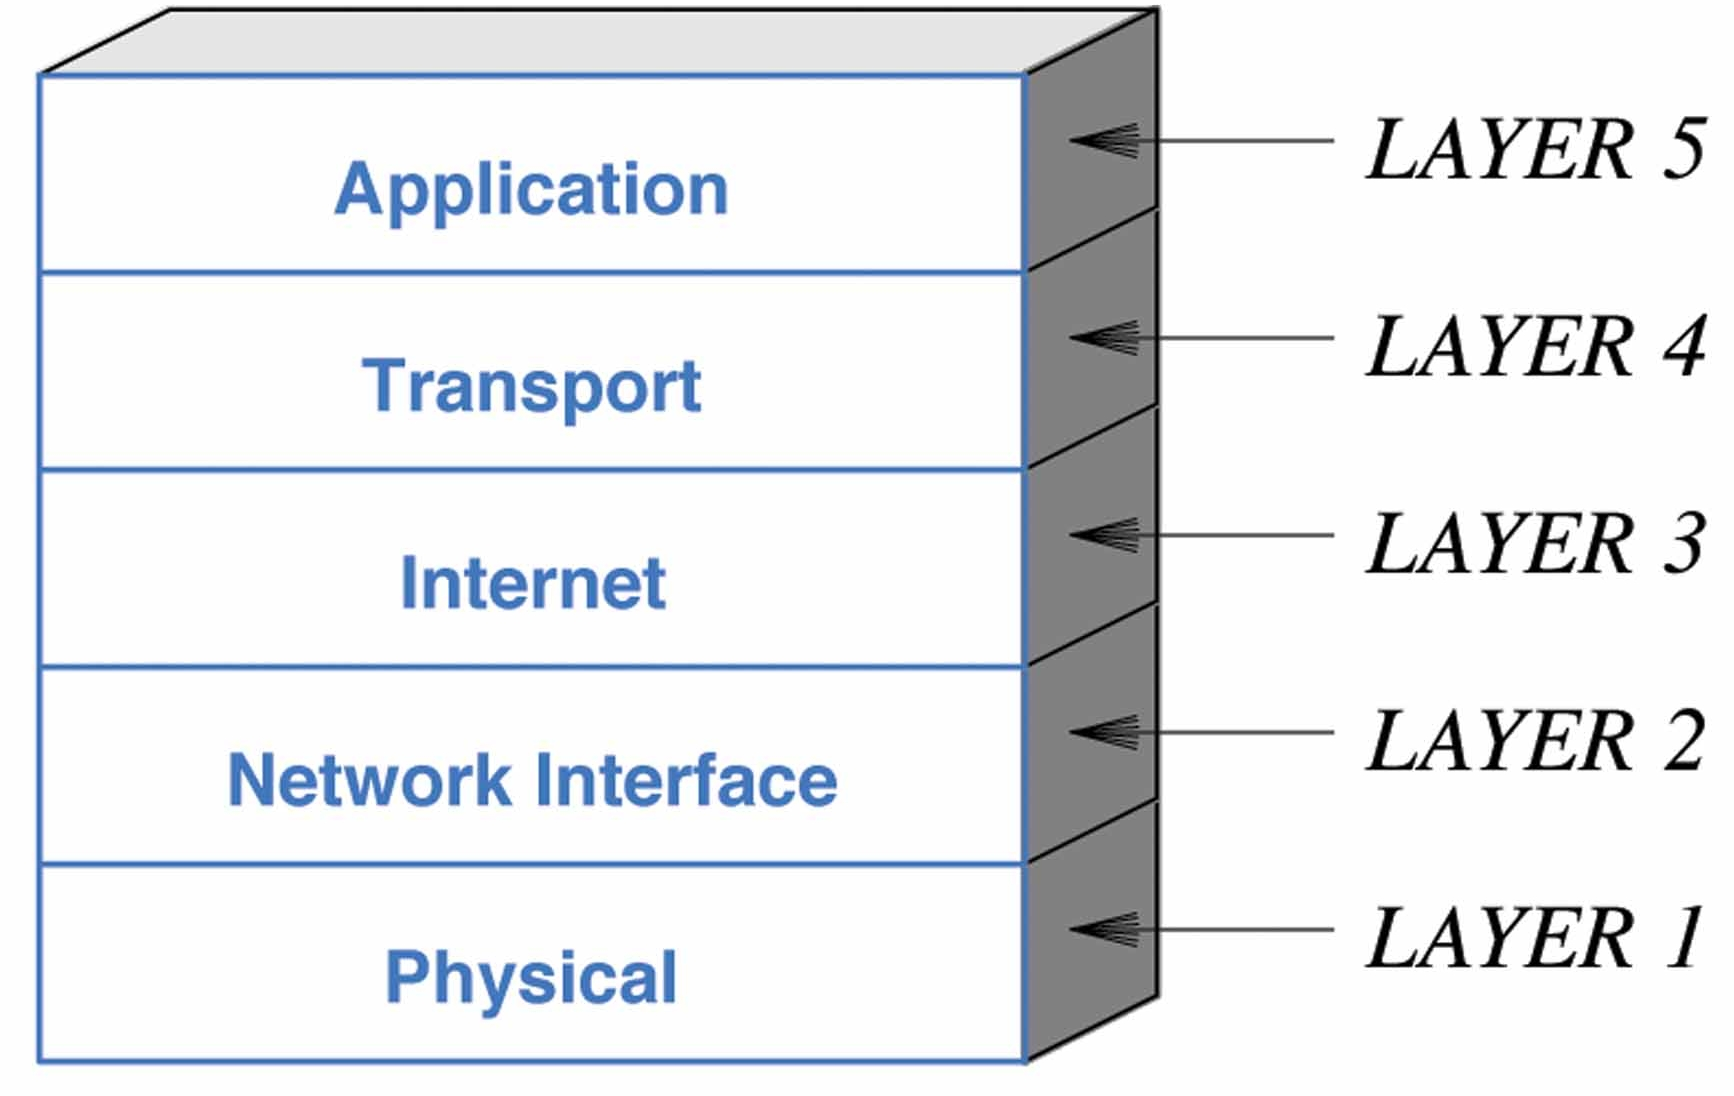
\includegraphics[scale=0.15]{assets/tcp-ip-stack.jpg}
	\end{center}
	Descrivendo brevemente i livelli del TCP/IP:
	\begin{itemize}
		\item \textbf{Livello applicazione}: prevede la comunicazione tra due processi (programmi eseguiti a questo livello) tramite scambio di messaggi end-to-end, anche se la comunicazione reale attraversa tutti i livelli del modello di rete. Per comunicare, un processo invia una richiesta e ne riceve una risposta. Esistono vari protocolli predefiniti per questo scopo, come HTTP per il web, SMTP per la posta elettronica, FTP per il trasferimento di file, TELNET e SSH per l'accesso remoto, e DNS per la risoluzione degli indirizzi.

		\item \textbf{Livello trasporto}: gestisce la comunicazione end-to-end tra host. Riceve i messaggi dal livello applicazione, li incapsula in segmenti e li invia all'host destinatario. Sebbene esista già una connessione end-to-end a livello applicazione, il livello di trasporto è indipendente e offre protocolli diversi, ciascuno adatto a specifiche esigenze. I principali protocolli sono TCP e UDP. TCP è orientato alla connessione, garantisce controllo del flusso, degli errori e della congestione, mentre UDP è connectionless, semplice e non offre controlli, ideale per applicazioni che richiedono velocità e brevi messaggi senza ritrasmissione.

		\item \textbf{Livello rete}: ha il compito di inviare i pacchetti dall'host sorgente a quello destinatario, occupandosi dell'instradamento e inoltro tramite router. La comunicazione è host-to-host e il protocollo principale è l'IP, che definisce il formato dei pacchetti (datagrammi) e degli indirizzi. L'IP è connectionless e non offre controllo del flusso, congestione o errori, delegando questi compiti al livello di trasporto. Il livello di rete gestisce anche protocolli per instradamento unicast e multicast, e protocolli di supporto come ICMP, IGMP e DHCP per segnalazioni e gestione degli indirizzi.

		\item \textbf{Livello collegamento}: trasferisce i pacchetti attraverso i collegamenti fisici determinati dai router, come LAN cablate, wireless o WAN. Ogni tipo di link può utilizzare protocolli differenti, ma l'obiettivo è sempre trasferire il pacchetto attraverso il collegamento. L'architettura TCP/IP non definisce protocolli specifici per questo livello, supportando sia standard che protocolli proprietari. I pacchetti a livello di collegamento sono chiamati frame, e alcuni protocolli possono fornire servizi come rilevazione e correzione degli errori.

		\item \textbf{Livello fisico}: trasferisce i singoli bit di un frame attraverso un link fisico, come cavi o etere. Anche se si tratta del livello più basso nel modello TCP/IP, la comunicazione tra dispositivi a questo livello è logica, poiché il mezzo trasmissivo sottostante trasporta segnali elettrici o ottici, non bit. I bit del frame vengono trasformati in segnali per essere inviati, ma possiamo comunque immaginare che l'unità logica trasmessa tra i dispositivi sia il bit.
	\end{itemize}

	\subsection{Incapsulamento e decapsulamento}
	Quando un messaggio viene inviato da un host a un altro, il messaggio viene incapsulato in un PDU a ogni livello del modello TCP/IP. Questo processo è chiamato incapsulamento. Quando il messaggio arriva all'host destinatario, il messaggio viene decapsulato a ogni livello del modello TCP/IP. Questo processo è chiamato decapsulamento. Ogni livello del modello TCP/IP aggiunge un'intestazione al messaggio, che contiene informazioni di controllo e dati. L'intestazione viene rimossa durante il decapsulamento. L'incapsulamento e il decapsulamento sono processi simmetrici.
	Descrivendo nel dettaglio il percorso di incapsulamento:
	\begin{enumerate}
		\item A livello applicazione i dati da scambiare vengono chiamati messaggi. Un messaggio non contiene alcun header o trailer. Il messaggio viene passato al livello di trasporto.

		\item Il livello trasporto considera il messaggio ricevuto come payload che deve trasportare e aggiunge l'header di livello trasporto che contiene varie informazioni per la gestione del messaggio a quel livello. Al livello di trasporto il risultato dell'incapsulamento viene chiamato segmento. Il segmento viene passato al livello di rete.

		\item Il livello di rete considera il segmento ricevuto come payload e aggiunge l'header di livello di rete che contiene varie informazioni per la gestione del messaggio a quel livello quali gli indirizzi degli host sorgente e destinatario e altre informazioni utili per il controllo degli errori. Al livello di rete il risultato dell'incapsulamento viene chiamato datagramma. Il datagramma viene passato al livello di collegamento.
		
		\item Il livello di collegamento considera il datagramma ricevuto come payload e aggiunge l'header di livello di collegamento che contiene varie informazioni per la gestione del messaggio a quel livello quali gli indirizzi MAC degli host sorgente e destinatario e altre informazioni utili. Al livello di collegamento il risultato dell'incapsulamento viene chiamato frame. Il frame viene passato al livello fisico per la trasmissione.
	\end{enumerate}
	\begin{center}
		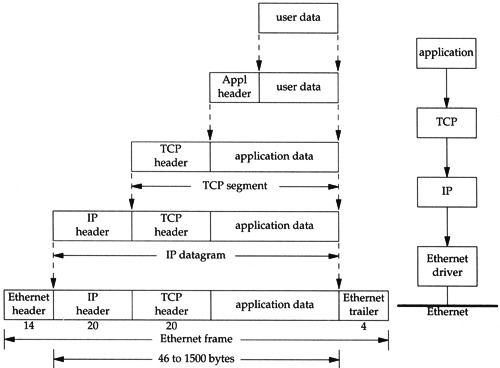
\includegraphics[scale=0.50]{assets/tcp-encapsulation.jpg} 
	\end{center}
	Nel decapsulamento il processo è inverso: il frame viene ricevuto dal livello fisico, il frame viene passato al livello di collegamento, l'header di livello di collegamento viene rimosso e il payload viene passato al livello di rete, l'header di livello di rete viene rimosso e il payload viene passato al livello di trasporto, l'header di livello di trasporto viene rimosso e il payload viene passato al livello applicazione. Durante questa fase vengono effettuati i controlli di errore e di sicurezza.

	\subsection{Indirizzamento}
	Un indirizzo è un identificatore univoco che consente di identificare un host o un dispositivo di rete durante la comunicazione, sia esso un host, un router o un altro dispositivo e sia sorgente o destinatario. Ogni livello del modello TCP/IP utilizza un indirizzo specifico per identificare i dispositivi.
	\begin{center}
		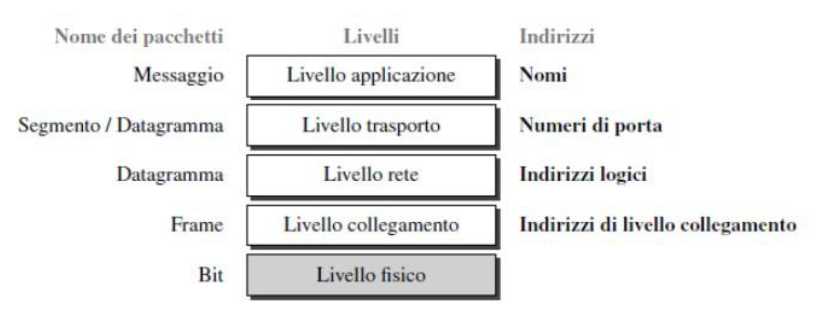
\includegraphics[scale=0.50]{assets/tcp-address.png}
	\end{center}
	Tipicamente, a livello applicazione vengono utilizzati nomi simbolici per specificare il sito che fornisce i servizi o l'indirizzo di posta elettronica.
	\vspace{\baselineskip}\\
	A livello trasporto gli indirizzi vengono chiamati numeri di porta e indicano i programmi sorgente e destinazione del livello applicazione. I numeri di porta sono indirizzi locali che consentono di distinguere i vari programmi in esecuzione concorrente.
	\vspace{\baselineskip}\\
	A livello rete gli indirizzi sono globali in ambito Internet: un indirizzo di livello rete deve identificare univocamente il collegamento di un dispostitivo a Internet.
	\vspace{\baselineskip}\\
	A livello di collegamento, gli indirizzi sono chiamati indirizzi MAC e sono definiti localmente, ognuno dei quali identifica una specifica interfaccia di rete.

	\subsection{Multiplexing e Demultiplexing}
	Considerando la presenza di più protocolli per livello nello stack TCP/IP, è necessario eseguire il multiplexing alla sorgente e il demultiplexing alla destinazione. Multiplexing significa che un protocollo di un livello può incapsulare, uno alla volta, i pacchetti ottenuti da più protocolli del livello immediatamente superiore. Demultiplexing significa che un protocollo può decapsulare e consegnare i pacchetti a più protocolli del livello immediatamente superiore.
	\vspace{\baselineskip}\\
	Per poter effettuare le operazioni di multiplexing e demultiplexing, un protocollo deve avere un campo nel proprio header per identificare a quale protocollo appartengano i pachetti incapsulati.
	\begin{center}
		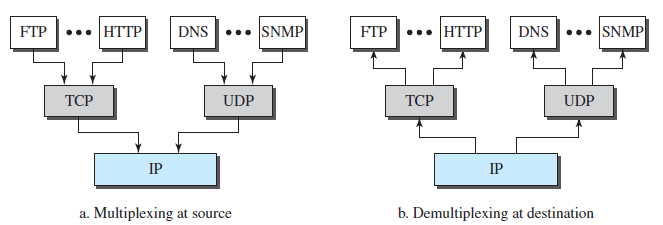
\includegraphics[scale=0.50]{assets/tcp-multiplexing.jpg}
	\end{center}

	\section{Il modello OSI}
	Il modello OSI (Open Systems Interconnection) è un modello a sette livelli che definisce la comunicazione tra dispositivi di rete. Il modello OSI è stato sviluppato dall'ISO (International Organization for Standardization) per standardizzare la comunicazione tra dispositivi di rete. Il modello OSI è stato progettato per essere aperto, cioè indipendente dall'hardware e dal software, consentendo a qualsiasi dispositivo di comunicare con qualsiasi altro dispositivo. Il modello OSI è stato progettato per essere flessibile e scalabile, consentendo di aggiungere nuovi livelli o modificare i livelli esistenti senza dover modificare l'intero modello. Non è un protocollo, ma un modello concettuale che definisce i concetti e le funzionalità necessarie per la comunicazione tra dispositivi di rete.
	\vspace{\baselineskip}\\
	Inizialmente, si pensava che il modello OSI avrebbe rimpiazzato lo stack protocollare TCP/IP. In realtà questo non è avvenuto per varie ragioni, tra le quali:
	\begin{itemize}
		\item lo stack TCP/IP era già ampiamente diffuso e si erano dedicate molte risorse alla sua implementazione e alla sua diffusione;
		\item alcuni livelli nel modello OSI, come presentazione e sessione, non sono mai stati completamente specificati;
		\item i test di implementazione del modello OSI non riuscirono a dimostrare delle prestazioni tali da giustificarne l'adozione su larga scala andando a sostituire lo stack TCP/IP. 
	\end{itemize}
	\begin{center}
		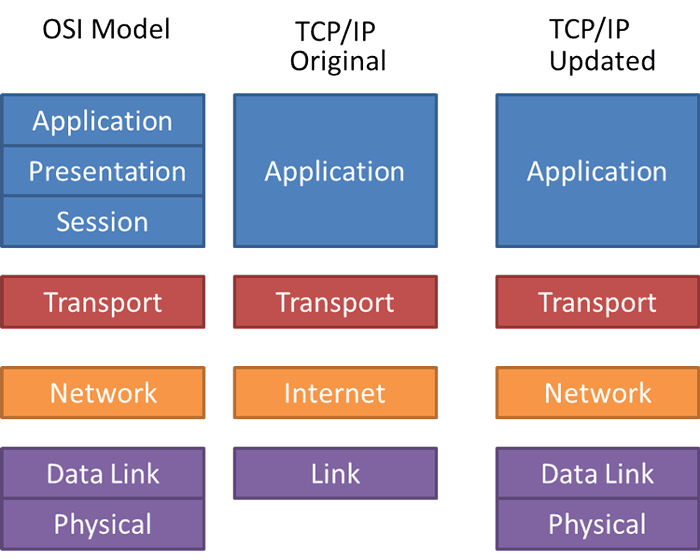
\includegraphics[scale=0.24]{assets/isoosi-vs-tcpip.png}
	\end{center}

	\section{Storia di Internet}
	Internet è nata negli anni '60 come progetto di ricerca del Dipartimento della Difesa degli Stati Uniti, chiamato ARPANET. ARPANET era una rete sperimentale che collegava quattro università negli Stati Uniti. ARPANET utilizzava la commutazione di pacchetto e il protocollo NCP (Network Control Protocol) per la comunicazione. Nel 1974, Vinton Cerf e Bob Kahn svilupparono il protocollo TCP (Transmission Control Protocol) e il protocollo IP (Internet Protocol) per sostituire NCP. Questi protocolli sono stati successivamente combinati in TCP/IP. Nel 1983, ARPANET passò a TCP/IP e divenne la rete Internet. Nel 1990, Tim Berners-Lee sviluppò il World Wide Web, che rese Internet accessibile a tutti. Nel 1993, il browser Mosaic rese il World Wide Web popolare. Nel 1995, Internet divenne commerciale e il numero di utenti crebbe rapidamente. Nel 2000, la bolla delle dot-com scoppiò, ma Internet continuò a crescere. Nel 2007, Apple lanciò l'iPhone, che rese Internet mobile. Nel 2010, Instagram e Pinterest furono lanciati, portando l'era dei social media. Nel 2015, la FCC adottò la neutralità della rete, garantendo che tutti i dati fossero trattati allo stesso modo. Nel 2020, la pandemia di COVID-19 accelerò la digitalizzazione e l'uso di Internet.

	\section{Amministazione della rete Internet}
	Internet è gestita da diverse organizzazioni, tra cui:
	\begin{itemize}
		\item \textbf{ICANN (Internet Corporation for Assigned Names and Numbers)}: è un'organizzazione no-profit che si occupa della gestione degli indirizzi IP e dei nomi di dominio. ICANN assegna gli indirizzi IP e i nomi di dominio ai registri regionali e ai registrar.
		\item \textbf{IETF (Internet Engineering Task Force)}: è un'organizzazione che sviluppa e standardizza i protocolli Internet. IETF è responsabile della definizione dei protocolli TCP/IP e di altri protocolli Internet.
		\item \textbf{ISOC (Internet Society)}: è un'organizzazione che promuove lo sviluppo e l'uso di Internet. ISOC si occupa di questioni di politica Internet e di educazione.
		\item \textbf{IANA (Internet Assigned Numbers Authority)}: è un'organizzazione che assegna gli indirizzi IP e i nomi di dominio. IANA è responsabile della gestione degli indirizzi IP e dei nomi di dominio.
		\item \textbf{IAB (Internet Architecture Board)}: è un'organizzazione che sovraintende lo sviluppo e la gestione dell'architettura Internet. IAB è responsabile della definizione dell'architettura Internet e della gestione dei protocolli Internet.
		\item \textbf{IRTF (Internet Research Task Force)}: è un'organizzazione che si occupa della ricerca e dello sviluppo di nuove tecnologie Internet. IRTF è responsabile della ricerca e dello sviluppo di nuove tecnologie Internet.
		\item \textbf{NIC (Network Information Center)}: è un'organizzazione che fornisce informazioni e servizi Internet. NIC è responsabile della registrazione degli indirizzi IP e dei nomi di dominio.
	\end{itemize}

	\chapter{Le architetture parallele}
	Le architetture dei computer possono essere suddivise in due principali categorie: quelle monolitiche, come i tipici sistemi monoprocessore, e quelle parallele. In un'architettura monolitica, un singolo processore gestisce la maggior parte delle operazioni e, sebbene ci possano essere dei coprocessori dedicati a compiti specifici (ad esempio, la gestione dei calcoli in virgola mobile o delle operazioni grafiche), essi agiscono principalmente come supporto al processore centrale, che resta il cuore dell'elaborazione.
	\vspace{\baselineskip}\\
	Le architetture parallele, al contrario, sfruttano più processori che lavorano contemporaneamente su più istruzioni. Questo consente di distribuire il carico di lavoro su diverse unità di elaborazione, che possono eseguire parti diverse dello stesso programma o programmi completamente separati. Tali architetture sono particolarmente utili per eseguire compiti computazionalmente intensivi o per affrontare grandi quantità di dati, come accade nelle reti di calcolatori (cluster) o nei supercomputer.
	\vspace{\baselineskip}\\
	Gli obiettivi delle architetture parallele includono non solo il miglioramento delle prestazioni del sistema complessivo, ma anche l'ottimizzazione del rapporto costo/prestazioni. Più processori che lavorano in parallelo permettono di ridurre i tempi di esecuzione di compiti complessi, migliorando l'efficienza e consentendo di risolvere problemi di dimensioni maggiori nello stesso arco di tempo. Ad esempio, in ambito scientifico, elaborazioni che richiederebbero giorni su un singolo processore possono essere completate in poche ore sfruttando il parallelismo.
	\vspace{\baselineskip}\\
	Un altro beneficio fondamentale delle architetture parallele è la scalabilità: aumentando il numero di processori, è possibile aumentare la capacità di elaborazione del sistema. Tuttavia, è importante notare che non tutti i problemi sono "parallelizzabili" allo stesso modo. Alcune operazioni richiedono un'elaborazione sequenziale e non beneficiano dell'aggiunta di nuovi processori. Per questo motivo, lo sviluppo di algoritmi efficienti che possano sfruttare al meglio le risorse parallele è un'area di ricerca cruciale nel campo dell'informatica.
	\\\\
	Un aspetto fondamentale per comprendere meglio le architetture parallele è l'analisi della \textbf{Tassonomia di Flynn}.
	
	\section{Tassonomia di Flynn}
	La tassonomia di Flynn è una classificazione dei sistemi di elaborazione in base alla modalità con cui gestiscono le istruzioni e i dati. Proposta da Michael J. Flynn nel 1966, la tassonomia di Flynn definisce quattro categorie principali di architetture parallele, basate su due dimensioni: il flusso di istruzioni e il flusso di dati. Queste due dimensioni possono essere singole o multiple, portando a quattro possibili combinazioni.

	\begin{center}
		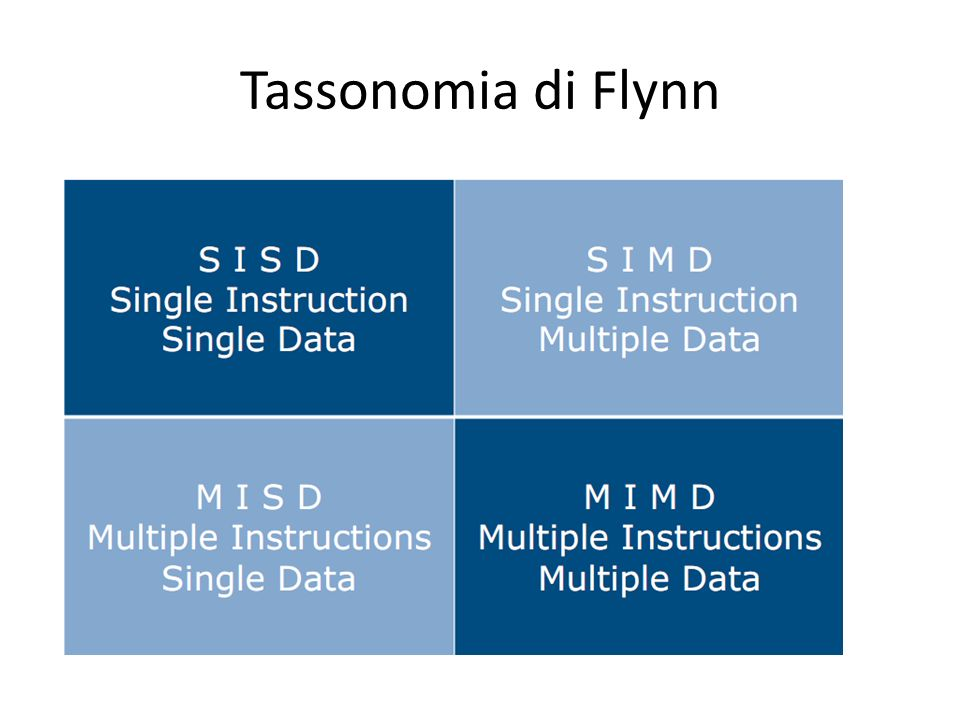
\includegraphics[scale=0.30]{assets/flynn-taxonomy.jpg}
	\end{center}

	\subsection{SISD (Single Instruction, Single Data)}
	Un sistema SISD è un sistema monoprocessore tradizionale, in cui un singolo processore esegue una singola istruzione su un singolo set di dati alla volta in un singolo istante di tempo. Questo è il modello classico dei computer monoprocessore, in cui il processore esegue sequenzialmente le istruzioni del programma su un singolo flusso di dati. Questo modello è adatto per applicazioni sequenziali e non sfrutta il parallelismo per migliorare le prestazioni.

	\subsection{SIMD (Single Instruction, Multiple Data)}
	Un sistema SIMD è un sistema in cui un'unica istruzione viene eseguita su più set di dati in un singolo istante di tempo. In un sistema SIMD, un'istruzione viene trasmessa a più unità di elaborazione, ciascuna delle quali opera su un diverso set di dati. Questo modello è particolarmente adatto per applicazioni in cui è possibile eseguire la stessa operazione su un grande volume di dati in parallelo, come nel caso di operazioni vettoriali o matriciali. I processori grafici (GPU) sono un esempio di architetture SIMD, in cui un'istruzione viene eseguita su più core contemporaneamente.

	\subsection{MISD (Multiple Instruction, Single Data)}
	Un sistema MISD è un sistema in cui più istruzioni vengono eseguite su un singolo set di dati in un singolo istante di tempo. E' un sistema ipotetico poichè non esistono applicazioni reali che sfruttino questa architettura. Tuttavia, è possibile immaginare scenari in cui più processori eseguono operazioni diverse sullo stesso set di dati, ad esempio per controllare la coerenza dei dati o per eseguire operazioni di sicurezza.

	\subsection{MIMD (Multiple Instruction, Multiple Data)}
	Un sistema MIMD è un sistema in cui più istruzioni vengono eseguite su più set di dati in parallelo. In un sistema MIMD, ogni processore esegue un'istruzione indipendente su un proprio set di dati, consentendo di eseguire operazioni diverse contemporaneamente. Questo modello è ampiamente utilizzato nelle architetture parallele, come i cluster di calcolatori, i supercomputer e i sistemi multiprocessore. In un sistema MIMD, i processori possono eseguire programmi diversi o parti diverse dello stesso programma in parallelo, migliorando le prestazioni complessive del sistema. Nell'ambito di questa classe, è possibile distinguere due ulteriori classi, tenendo conto della cooperazione progettuale tra i vari processori:
	\begin{itemize}
		\item \textbf{Sistemi in collegamento LASCO}: nel quale i processori sono situati in macchine differenti le quali, a loro volta, sono collegate tra loro da una rete di comunicazione di computer. Ciascun processore ha una propria RAM, possiede unità di I/O indipendenti e ha un proprio OS. I processori di questo sistema possono lavorare indipendentemente o cooperare tra loro tramite la linea di commutazione e quindi condividere risorse, quali archivi di dati memorizzati in memoria di massa.
		\item \textbf{Sistemi in collegamento STRETTO}: nel quale i processori sono situati in una singola macchina, condividono la stessa RAM e le stesse unità di I/O e sono gestite dallo stesso OS. LA velocità di dialogo fra di essi è maggiore rispetto ai sistemi in collegamento lasco poichè non è necessario passare attraverso la rete di comunicazione di computer. 
	\end{itemize}

	\chapter{Storage in rete}
	Nel contesto informatico, lo \textit{storage} si riferisce all'insieme di dispositivi e tecnologie utilizzati per memorizzare dati in modo permanente o temporaneo, consentendo il recupero e la gestione delle informazioni quando necessario. In un ambiente \textit{stand-alone}, ovvero un sistema isolato senza connessione a una rete, l'unica opzione di archiviazione è rappresentata dal disco fisso interno al computer, su cui vengono salvati i dati localmente. Questa configurazione presenta però notevoli limiti, sia in termini di spazio di archiviazione, che dipende dalla capacità fisica del disco installato, sia di flessibilità e accessibilità.
	\vspace{\baselineskip}\\
	In un ambiente di rete, invece, lo storage assume un valore più ampio e versatile, poiché permette di accedere a unità di archiviazione esterne e remote senza che siano fisicamente collegate al singolo dispositivo in uso. Per rispondere a questa necessità, sono state sviluppate diverse tecnologie che permettono di aggregare più unità disco in un’infrastruttura centralizzata, espandendo la capacità di archiviazione e ottimizzando i costi di gestione. Le configurazioni di storage di rete più diffuse possono essere classificate in tre categorie:
	\begin{itemize}
		\item \textbf{DAS} (Direct Attached Storage)
		\item \textbf{NAS} (Network Attached Storage)
		\item \textbf{SAN} (Storage Area Network)
	\end{itemize}
	
	\section{DAS}
	Il sistema \textit{Direct Attached Storage} (DAS) collega l'apparato di archiviazione direttamente a un server, senza utilizzare la rete. In pratica, il DAS è il disco fisso di un server che funziona come dispositivo di storage dedicato. La resilienza ai guasti (\textit{fault tolerance}) viene garantita tramite l’uso di configurazioni \textit{RAID} (\textit{Redundant Array of Independent Disks}), che combinano più dischi in un’unità logica unica, riducendo il rischio di perdita di dati in caso di guasto di uno o più dischi. I sistemi RAID permettono anche la sostituzione dei dischi "a caldo" (\textit{hot swap}), ossia senza interruzione del servizio. Tuttavia, i DAS presentano una limitata scalabilità e, nel caso in cui il server vada riavviato, l’accesso ai dati viene sospeso, generando tempi di inattività.
	
	\section{NAS}
	Con il \textit{Network Attached Storage} (NAS), l’unità di archiviazione diventa un vero e proprio server dotato di sistema operativo e con una scheda di rete per connettersi alla LAN aziendale. A ogni NAS viene assegnato un indirizzo IP, rendendone possibile la gestione tramite un normale web browser da qualsiasi computer connesso alla rete. Il collegamento alla rete consente di posizionare il NAS in qualsiasi punto della LAN, connesso fisicamente allo switch della rete come ogni altro nodo. Il NAS è quindi facilmente accessibile a più dispositivi in rete e ideale per un ambiente con diversi utenti che richiedono accesso condiviso ai file.
	
	\section{SAN}
	La \textit{Storage Area Network} (SAN) è una rete ad alta velocità che collega esclusivamente dispositivi di memorizzazione, creando una rete locale di server di archiviazione. Una SAN permette l’accesso centralizzato ai dati da parte di tutti i computer collegati alla LAN o MAN aziendale, risultando particolarmente utile in grandi organizzazioni che devono supportare servizi aziendali intensivi, come applicazioni server e database. Le SAN includono sistemi avanzati di protezione dei dati e componenti hardware ridondanti per garantire la massima sicurezza e disponibilità dei dati. Inoltre, i dispositivi SAN possono essere ampliati “a caldo” grazie alle interfacce ad alta velocità, consentendo di aumentare la capacità senza interruzioni del servizio e senza alcun impatto per gli utenti. A differenza di NAS e DAS, le SAN sono progettate per una scalabilità maggiore.

	\chapter{Cloud Computing}
	Il \textit{cloud computing} rappresenta un modello di erogazione di servizi informatici offerti su richiesta (\textit{on demand}) tramite Internet. Con il cloud, le risorse IT - come capacità di calcolo, archiviazione e software - vengono fornite da un fornitore esterno e messe a disposizione dell’utente finale senza richiedere infrastrutture locali.
	In modo simile a come l'energia elettrica è fornita attraverso una rete, il cloud rende disponibili risorse informatiche in modo economico e immediato. Gli utenti possono accedere ai servizi cloud da qualsiasi luogo connesso a Internet e pagano solo per le risorse effettivamente utilizzate. 
	Essendo un ambiente multiutente, il cloud deve assicurare:
	\begin{itemize}
		\item una gestione sicura dell’identità e dell’accesso degli utenti;
		\item un’allocazione dinamica delle risorse per ogni utente;
		\item l’accesso esclusivo alle risorse riservate a ciascun utente;
		\item una protezione efficace contro interferenze tra attività di utenti diversi.
	\end{itemize}
	Secondo il \textit{NIST} (National Institute of Standards and Technology), il cloud computing presenta:
	\begin{itemize}
		\item cinque caratteristiche essenziali;
		\item tre modelli di servizio;
		\item quattro modelli di distribuzione.
	\end{itemize}

	\section{Caratteristiche principali del Cloud}
	Un servizio si definisce \textit{cloud} se possiede le seguenti caratteristiche:
	\begin{enumerate}
		\item \textbf{On-demand self-service}: l'utente accede in modo automatico a risorse come capacità di calcolo e archiviazione, senza dover richiedere interventi manuali da parte del fornitore.
		\item \textbf{Broad network access}: le funzionalità devono essere disponibili in rete e accessibili tramite dispositivi standard come smartphone, tablet o computer.
		\item \textbf{Resource pooling}: le risorse (elaborazione, memoria, larghezza di banda) devono poter essere assegnate e riassegnate dinamicamente in base alla domanda degli utenti.
		\item \textbf{Rapid elasticity}: le risorse devono poter essere rapidamente allocate e scalate, in modo da adattarsi alle variazioni della domanda.
		\item \textbf{Measured service}: il consumo delle risorse deve essere monitorato e misurato, permettendo un modello di pagamento basato sull'uso effettivo.
	\end{enumerate}

	\section{Modelli di Servizio nel Cloud}
	I modelli di servizio del cloud si distinguono in base alla tipologia di risorse messe a disposizione:
	\begin{itemize}
		\item \textbf{SaaS} (\textit{Software-as-a-Service}): il provider offre software applicativi accessibili tramite Internet, come Google Workspace e Microsoft Office 365.
		\item \textbf{PaaS} (\textit{Platform-as-a-Service}): il provider mette a disposizione una piattaforma per lo sviluppo di applicazioni, con strumenti, librerie e servizi integrati. Questo modello è destinato principalmente agli sviluppatori.
		\item \textbf{IaaS} (\textit{Infrastructure-as-a-Service}): il provider fornisce l’infrastruttura hardware di base (server, storage, reti), lasciando al cliente la possibilità di installare e gestire il proprio software.
	\end{itemize}

	\subsection{SaaS}
	Nel modello SaaS, il software viene erogato come servizio e gli utenti vi accedono tramite Internet, spesso pagando un abbonamento mensile o annuale. In questo modo, non è necessario installare o aggiornare il software sui propri dispositivi.

	\subsection{PaaS}
	Il PaaS è rivolto a sviluppatori che desiderano creare applicazioni senza preoccuparsi della gestione dell’infrastruttura. Il fornitore offre una \textit{solution stack} completa con linguaggi di programmazione, librerie e ambienti di sviluppo.

	\subsection{IaaS}
	L’IaaS fornisce l’infrastruttura IT fondamentale, come server e storage, permettendo al cliente di configurare e gestire il proprio software e i sistemi operativi. Questo modello offre grande flessibilità a chi ha bisogno di controllo completo sull’infrastruttura.

	\section{Modelli di Distribuzione del Cloud}
	A seconda della modalità di distribuzione e degli utenti destinatari, il cloud computing può essere:
	\begin{enumerate}
		\item \textbf{Private Cloud}: un'infrastruttura cloud riservata a una singola organizzazione.
		\item \textbf{Community Cloud}: infrastruttura condivisa tra organizzazioni con obiettivi comuni.
		\item \textbf{Public Cloud}: servizi resi disponibili al pubblico, accessibili da chiunque tramite Internet.
		\item \textbf{Hybrid Cloud}: una combinazione di più modelli di cloud, che consente all’organizzazione di mantenere una parte dell’infrastruttura privata e di affidarsi al cloud pubblico per altri servizi.
	\end{enumerate}

	\section{Vantaggi e Svantaggi del Cloud}
	I vantaggi del cloud computing si riassumono in:
	\begin{itemize}
		\item \textbf{Flessibilità}: gli utenti possono adattare i servizi alle proprie esigenze, accedendo da qualunque luogo connesso a Internet.
		\item \textbf{Efficienza}: l'infrastruttura cloud permette un uso ottimale delle risorse, in modo da rispondere sia ai picchi di utilizzo che ai periodi di attività ridotta.
		\item \textbf{Valore strategico}: il cloud permette alle organizzazioni di ridurre i costi operativi, concentrandosi sulle proprie attività principali.
	\end{itemize}
	Lo svantaggio principale può essere rappresentato dalla possibile riduzione delle prestazioni rispetto a un server locale, ma generalmente i servizi cloud sono progettati per offrire prestazioni coerenti con le aspettative aziendali.

	\chapter{Rilevazione e correzione degli errori}
	La rilevazione e la correzione degli errori sono due tecniche fondamentali per garantire l'integrità dei dati trasmessi su una rete di calcolatori. La rilevazione degli errori consiste nel determinare se un errore è presente nei dati trasmessi, mentre la correzione degli errori consiste nell'identificare e correggere gli errori rilevati. Esistono diverse tecniche per la rilevazione e la correzione degli errori, ciascuna con vantaggi e svantaggi specifici. In generale, la scelta della tecnica più adatta dipende dalle esigenze specifiche dell'applicazione e dalle risorse disponibili.

	\section{Metodi di rilevazione degli errori}
	\subsection{Bit di Parità}
	Il bit di parità è una tecnica di rilevazione degli errori che consiste nell'aggiungere un bit di controllo ai dati trasmessi. Il bit di parità può essere 0 o 1, a seconda del numero di bit a 1 nei dati. Se il numero di bit a 1 è pari, il bit di parità è 0, altrimenti è 1.
	\vspace{\baselineskip}\\
	Questo viene calcolato effettuando uno XOR bitwise tra tutti i bit dei dati. Sia M il messaggio da inviare composto da 8 bit: $M = m_1m_2m_3m_4m_5m_6,m_7m_8$. Il bit di parità è calcolato come:
	\[
		m_9 = m_1 \oplus m_2 \oplus m_3 \oplus m_4 \oplus m_5 \oplus m_6 \oplus m_7 \oplus m_8
	\]
	Dopo aver calcolato il bit di parità, il mittente invierà il messaggio $M' = m_1m_2m_3m_4m_5m_6,m_7m_8m_9$ di 9 bit. 
	\vspace{\baselineskip}\\
	Quando i dati vengono trasmessi, il ricevitore riceverà il messaggio $M'' = M'$ e calcolerà il bit di parità sui 9 bit ricevuti effettuando uno XOR bitwise tra tutti i bit. Se il bit di parità calcolato è uguale a 0, non ci sono errori nei dati trasmessi. Se il bit di parità calcolato è uguale a 1, si è verificato un errore nei dati trasmessi. In caso di errore il ricevitore può richiedere la ritrasmissione dei dati o può scartare i dati corrotti.
	\vspace{\baselineskip}\\
	Per convenzione, il bit di parità è sempre aggiunto nella posizione del bit meno significativo.
	\vspace{\baselineskip}\\
	Questa tecnica ouò rilevare errori singoli, ma non può correggerli. Inoltre, se due errori si verificano nello stesso messaggio, il bit di parità non sarà in grado di rilevarli. Per questo motivo, il bit di parità è spesso utilizzato in combinazione con altre tecniche di rilevazione e correzione degli errori.
	\vspace{\baselineskip}\\
	Ricordiamo la tavola di verità dello XOR:
	\begin{center}
		\begin{tabular}{|c|c|c|}
			\hline
			A & B & A $\oplus$ B \\
			\hline
			0 & 0 & 0 \\
			0 & 1 & 1 \\
			1 & 0 & 1 \\
			1 & 1 & 0 \\
			\hline
		\end{tabular}
	\end{center}

	\paragraph{Esempio}
	Sia \textit{M} il messaggio da trasmettere ove \textit{M} $= m_1m_2m_3m_4m_5m_6,m_7m_8 =  01010100$. Il mittente calcola il bit di parità effettuando uno XOR tra tutti i bit del messaggio.
	\begin{equation*}
			m_9 = m_1 \oplus m_2 \oplus m_3 \oplus m_4 \oplus m_5 \oplus m_6 \oplus m_7 \oplus m_8 = 0 \oplus 1 \oplus 0 \oplus 1 \oplus 0 \oplus 1 \oplus 0 \oplus 0  = 1
	\end{equation*}
	Il messaggio da trasmettere è quindi $M' = m_1m_2m_3m_4m_5m_6,m_7m_8m_9 = 010101001$.
	\vspace{\baselineskip}
	Il ricevente calcola il bit di parità effettuando uno XOR tra tutti i bit del messaggio ricevuto.
	\begin{equation*}
		p = m_1 \oplus m_2 \oplus m_3 \oplus m_4 \oplus m_5 \oplus m_6 \oplus m_7 \oplus m_8 \oplus m_9 = 0 \oplus 1 \oplus 0 \oplus 1 \oplus 0 \oplus 1 \oplus 0 \oplus 0 \oplus 1 = 0
	\end{equation*}
	Il bit di parità calcolato è 0, quindi non ci sono errori nei dati trasmessi.

	\subsection{Internet Checksum}
	L'Internet Checksum è una tecnica di rilevazione degli errori utilizzata nei protocolli di rete, come l'IP e l'UDP. L'Internet Checksum viene calcolato dal mittente effettuando la somma in complemento a 1 di tutte le parole da 16 bit del messaggio, con eventuale padding e con eventuale riporto sommato al primo bit. Tale risultato viene poi posto nel campo di checksum dell'header del pacchetto. Il ricevente calcola la somma in complemento a 1 delle parole iniziali del pacchetto, compreso il checksum, e verifica che il risultato sia uguale a tutti 1. Se il risultato è diverso da tutti 1, si è verificato un errore nei dati trasmessi. Per semplicità assumeremo che la lunghezza del messaggio sia un multiplo di 32 bit.

	\paragraph{Esempio}
	Supponiamo di avere il seguente messaggio da inviare di 32 bit $M = 0101 0000 1111 0101 1111 0101 1010 1011$ che viene diviso in due parole da 16 bit $M' = 0101 0000 1111 0101$ e $M'' = 1111 0101 1010 1011$. Il mittente calcola la somma in complemento a 1 delle due parole.
	
	\begin{center}		
		\begin{tabular}{llllll}
		Riporti:         & \textit{1000} & \textit{0011} & \textit{1101} & \textit{1110} &   \\
		M':              & 0101          & 0000          & 1111          & 0101          & + \\
		M'':             & 1111          & 0101          & 1010          & 1011          &   \\
		\hline
		Risultato somma: & 0100          & 0110          & 1010          & 0001          &   \\
		Checksum C:        & 1011          & 1001          & 0101          & 1110          &  
		\end{tabular}
	\end{center}
	Il mittente invierà il messaggio $N = MC = 0101 0000 1111 0101 1111 0101 1010 1011 1011 1001 0101 1110$. Il ricevente poi dividerà il messaggio $N$ in parole da 16 bit $N' = 0101 0000 1111 0101$, $N'' = 1111 0101 1010 1011$ e $N''' = 0100 0110 1010 0001$ e calcolerà la somma in complemento a 1 delle tre parole. Per semplicità omettiamo il calcolo. Il risultato sarà $1111 1111 1111 1111$, che indica che non ci sono errori nei dati trasmessi.
	
	\section{Metodi di rilevamento correzione degli errori}
	\subsection{Codici di Hamming}
	I codici di Hamming sono una famiglia di codici di correzione degli errori che consentono di rilevare e correggere errori nei dati trasmessi. I codici di Hamming sono basati su una matrice di controllo che consente di individuare e correggere errori nei dati. I codici di Hamming sono utilizzati in molte applicazioni, come la memorizzazione dei dati su dischi rigidi, la trasmissione dei dati su reti di calcolatori e la memorizzazione dei dati nei computer. Rispetto al metodo del bit di parità, vengono aggiunti più bit di controllo per consentire la correzione degli errori. Per semplicità di spiegazione, limitiamo la nostra analisi al codice di Hamming che aggiunge 4 bit di controllo a un messaggio di 8 bit.
	\vspace{\baselineskip}\\
	Dato un messaggio M da inviare, il procedimento da applicare per ottenere il frame $M_s$ effettivamente trasmesso consiste nel sistemare i bit su una riglia di 12 bit, dove i bit di controllo sono posti nelle posizioni potenze di 2 (nel nostro caso 1, 2, 4 e 8). Le restanti posizioni vengono occupate in maniera ordinata dai bit del messaggio M.
	\begin{center}
		\begin{tabular}{|l|l|l|l|l|l|l|l|l|l|l|l|}
		\hline
		0001                 & 0010                 & 0011 & 0100                & 0101 & 0110 & 0111 & 1000                 & 1001 & 1010 & 1011 & 1100 \\ \hline
		$h_1$                   & $h_2$                   & $m_1$   & $h_3$                  & $m_2$   & $m_3$   & $m_4$   & $h_4$                   & $m_5$   & $m_6$   & $m_7$   & $m_8$   \\ \hline
		$2^0$ & $2^1$ &      & $2^2$ &      &      &      & $2^3$ &      &      &      &      \\ \hline
		\end{tabular}
	\end{center}
	ove $h_n$ indica il bit di controllo $\forall n \in \{1, 2, 3, 4\}$ e $m_n$ indica il bit del messaggio $\forall n \in \{1, 2, 3, 4, 5, 6, 7, 8\}$.
	\vspace{\baselineskip}\\
	Nello specifico:
	\begin{itemize}
		\item $h_1$ si trova in posizione 0001 del codice di Hamming e quindi controlla tutti i bit che nel valore binario della posizione occupata presentano un 1 nella posizione meno significativa. Infatti $h_1$ controlla i bit 001\textbf{1}, 010\textbf{1}, 011\textbf{1}, 100\textbf{1} e 101\textbf{1}, quindi $m_1$, $m_2$, $m_4$, $m_5$ e $m_7$.
		\item $h_2$ si trova in posizione 0010 del codice di Hamming e quindi controlla tutti i bit che nel valore binario della posizione occupata presentano un 1 nella seconda posizione da destra. Infatti $h_2$ controlla i bit 00\textbf{1}0, 01\textbf{1}0, 01\textbf{1}1, 10\textbf{1}0 e 10\textbf{1}1, quindi $m_1$, $m_3$, $m_4$, $m_6$ e $m_7$.
		\item $h_3$ si trova in posizione 0100 del codice di Hamming e quindi controlla tutti i bit che nel valore binario della posizione occupata presentano un 1 nella terza posizione da destra. Infatti $h_3$ controlla i bit 0\textbf{1}01, 0\textbf{1}10, 0\textbf{1}11 e 1\textbf{1}00, quindi $m_2$, $m_3$, $m_4$ e $m_8$.
		\item $h_4$ si trova in posizione 1000 del codice di Hamming e quindi controlla tutti i bit che nel valore binario della posizione occupata presentano un 1 nella posizione più significativa. Infatti $h_4$ controlla i bit \textbf{1}001, \textbf{1}010, \textbf{1}011 e \textbf{1}100 quindi $m_5$, $m_6$, $m_7$ e $m_8$.
	\end{itemize}
	Nel codice così costruito, ogni bit del messaggio da spedire è controllato da almeno due bit di controllo. I valori dei bit di controllo si ottengono mediante lo XOR tra tutti i bit controllati. Per cui avremo che:
	\begin{equation*}
		h_1 = m_1 \oplus m_2 \oplus m_4 \oplus m_5 \oplus m_7	
	\end{equation*}
	\begin{equation*}
		h_2 = m_1 \oplus m_3 \oplus m_4 \oplus m_6 \oplus m_7
	\end{equation*}
	\begin{equation*}
		h_3 = m_2 \oplus m_3 \oplus m_4 \oplus m_8
	\end{equation*}
	\begin{equation*}
		h_4 = m_5 \oplus m_6 \oplus m_7 \oplus m_8
	\end{equation*}
	Il ricevente riceverà $M_s$ e verificherà la sua correttezza mediante lo XOR tra tutti i bit controllati con il proprio bit controllore. Si determineranno $S_i$ somme di controllo, una per ogni bit di controllo $\forall i \in {1,2,3,4}$. 
	Si verificano due casi:
	\begin{itemize}
		\item $S_i = 0$: non ci sono errori nei dati trasmessi.
		\item Almeno una $S_i \neq 0$: si è verificato un errore nei dati trasmessi. In tal caso i valori $S_i$ letti nell'ordine $S_4S_3S_2S_1$ indicano la posizione del bit errato che per essere corretto andrà negato.
	\end{itemize}

	\paragraph{Esempio di messaggio corretto}
	Sia $M = 0100 1100$ il messaggio da inviare. Il mittente calcola i bit di controllo $h_1$, $h_2$, $h_3$ e $h_4$ come descritto in precedenza:
	\begin{equation*}
		h_1 = m_1 \oplus m_2 \oplus m_4 \oplus m_5 \oplus m_7 = 0 \oplus 1 \oplus 0 \oplus 1 \oplus 0 = 0
	\end{equation*}
	\begin{equation*}
		h_2 = m_1 \oplus m_3 \oplus m_4 \oplus m_6 \oplus m_7 = 0 \oplus 0 \oplus 0 \oplus 1 \oplus 0 = 1
	\end{equation*}
	\begin{equation*}
		h_3 = m_2 \oplus m_3 \oplus m_4 \oplus m_8 = 1 \oplus 0 \oplus 0 \oplus 0 = 1
	\end{equation*}
	\begin{equation*}
		h_4 = m_5 \oplus m_6 \oplus m_7 \oplus m_8 = 1 \oplus 1 \oplus 0 \oplus 0 = 0
	\end{equation*}
	Il messaggio da inviare sarà quindi $M_s = 0101 1000 1100$. Il ricevente calcolerà le somme di controllo $S_1$, $S_2$, $S_3$ e $S_4$ come descritto in precedenza:
	\begin{equation*}
		S_1 = m_1 \oplus m_2 \oplus m_4 \oplus m_5 \oplus m_7 \oplus h_1 = 0 \oplus 1 \oplus 0 \oplus 1 \oplus 0 \oplus 0 = 0
	\end{equation*}
	\begin{equation*}
		S_2 = m_1 \oplus m_3 \oplus m_4 \oplus m_6 \oplus m_7 \oplus h_2 = 0 \oplus 0 \oplus 0 \oplus 1 \oplus 0 \oplus 1 = 0
	\end{equation*}
	\begin{equation*}
		S_3 = m_2 \oplus m_3 \oplus m_4 \oplus m_8 \oplus h_3 = 1 \oplus 0 \oplus 0 \oplus 0 \oplus 1 = 0
	\end{equation*}
	\begin{equation*}
		S_4 = m_5 \oplus m_6 \oplus m_7 \oplus m_8 \oplus h_4 = 1 \oplus 1 \oplus 0 \oplus 0 \oplus 0 = 0
	\end{equation*}
	Non ci sono errori nei dati trasmessi.

	\paragraph{Esempio di messaggio con errore}
	Dall'esempio precedente, supponiamo che il messaggio $M = 0100 1100$ venga trasmesso con un errore nel bit $m_2$. Il messaggio da inviare sarà quindi $M_s = 0101 0000 1100$. Il ricevente calcolerà le somme di controllo $S_1$, $S_2$, $S_3$ e $S_4$ come descritto in precedenza:
	\begin{equation*}
		S_1 = m_1 \oplus m_2 \oplus m_4 \oplus m_5 \oplus m_7 \oplus h_1 = 0 \oplus 0 \oplus 0 \oplus 1 \oplus 0 \oplus 0 = 1
	\end{equation*}
	\begin{equation*}
		S_2 = m_1 \oplus m_3 \oplus m_4 \oplus m_6 \oplus m_7 \oplus h_2 = 0 \oplus 0 \oplus 0 \oplus 1 \oplus 0 \oplus 1 = 0
	\end{equation*}
	\begin{equation*}
		S_3 = m_2 \oplus m_3 \oplus m_4 \oplus m_8 \oplus h_3 = 0 \oplus 0 \oplus 0 \oplus 0 \oplus 1 = 1
	\end{equation*}
	\begin{equation*}
		S_4 = m_5 \oplus m_6 \oplus m_7 \oplus m_8 \oplus h_4 = 1 \oplus 1 \oplus 0 \oplus 0 \oplus 0 = 0
	\end{equation*}
	Le somme di controllo $S_1$ e $S_3$ sono diverse da 0, quindi si è verificato un errore nei dati trasmessi. I valori letti nell'ordine $S_4S_3S_2S_1$ indicano la posizione del bit errato che per essere corretto andrà negato. In questo caso la posizione del bit errato è 0101, che corrisponde al bit $m_2$.

	\chapter{Resilienza dei sistemi}
	La resilienza dei sistemi è la capacità di un sistema di resistere a guasti e malfunzionamenti e di riprendersi rapidamente da tali eventi. La resilienza è un aspetto fondamentale per garantire l'affidabilità e la disponibilità dei sistemi informatici, in particolare in ambienti critici come le reti di calcolatori, i data center e i sistemi di controllo industriale. La resilienza dei sistemi può essere ottenuta attraverso una combinazione di tecniche e strategie progettuali.

	\section{Backup e ripristino}
	Con il termine backup si indica il processo di messa in sicurezza delle informazioni di un sistema informatico attraverso la creazione di una o più copie dei dati, da utilizzare come recupero dei dati stessi in caso di eventi malevoli accidentali o intenzionali o semplice manutenzione del sistema. Un backup può anche risultare utile per proteggersi dai ransomware. È evidente che le copie devono essere conservate in siti geograficamente distanti tra loro in modo che eventuali incendi, terremoti, o altri eventi, non compromettano tutte le copie. Essi possono essere conservati anche in cloud. L'operazione di ripristino è il processo di recupero dei dati da una copia di backup in caso di perdita o danneggiamento dei dati originali. Il ripristino può essere effettuato su un sistema identico o su un sistema diverso, a seconda delle esigenze dell'applicazione e delle risorse disponibili.
	\vspace{\baselineskip}\\
	Una strategia potenzialmente vincente a salvaguardia dei propri dati non può non partire da una sana policy di backup dei dati. Il backup dei proprio dati è un’azione da eseguire regolarmente, quanto più frequentemente possibile, se non addirittura in tempo reale.
	\vspace{\baselineskip}\\
	Esistono diversi tipi di backup:
	\begin{itemize}
		\item \textbf{Backup completo}: duplicazione da zero di un intero set di dati. Sebbene sia considerato il metodo più affidabile, l’esecuzione di un backup completo non solo richiede molto tempo ma impone di avere a disposizione un 		numero elevato di dischi.
		\item \textbf{Backup incrementale}: generazione di una copia solamente dei dati che sono stati modificati rispetto al backup precedente, completo o incrementale che sia. La durata di tale processo è ovviamente inferiore alla durata di un backup completo, ma presenta lo svantaggio (in caso di back precedente completo) di rendere più complessa la fase di ripristino poichè bisognerà innanzitutto recuperare il backup completo e poi tutti i backup incrementali successivi.
		\item \textbf{Backup differenziale}:  è simile a un backup incrementale ma, in questo caso, ciò che viene salvato sono tutti i dati che sono stati modificati dall’ultimo backup completo. A differenza del backup incrementale, che salverà solo tutti i cambiamenti avvenuti dall’ultimo backup (sia esso completo o incrementale), il backup differenziale confronterà sempre i cambiamenti rispetto all’ultimo backup completo e salverà le differenze. Questa tipologia di backup richiede senz’altro più spazio rispetto al backup incrementale, ma consente di effettuare il ripristino completo più rapidamente richiedendo solo l’ultimo backup completo e l’ultimo backup
		differenziale.
	\end{itemize}

	\section{Disaster Recovery}
	Il \textit{disaster recovery} è il processo di ripristino di un sistema informatico in seguito a un evento catastrofico che ha causato la perdita o il danneggiamento dei dati. Tali eventi possono includere disastri naturali come incendi, alluvioni e terremoti, oltre a guasti hardware o software, attacchi informatici e altre circostanze che compromettono la disponibilità dei sistemi e l'integrità dei dati.
	\vspace{\baselineskip}\\
	L'obiettivo principale di una strategia di \textit{disaster recovery} è prevenire la perdita definitiva dei dati e garantire la continuità operativa. Questo si realizza tipicamente implementando un sito secondario dove tutti i dati vengono regolarmente salvati e possono essere recuperati in caso di emergenza. Una politica efficace di \textit{disaster recovery} si basa fortemente su processi di backup ben progettati.
	\vspace{\baselineskip}\\
	Nella scelta della strategia di backup, è fondamentale considerare due parametri chiave: il \textit{Recovery Point Objective} (RPO) e il \textit{Recovery Time Objective} (RTO). Questi due indicatori definiscono gli standard minimi di ripristino che un'azienda deve mantenere in caso di incidente.
	
	\begin{itemize}
		\item \textbf{RTO} (\textit{Recovery Time Objective}): rappresenta il tempo massimo entro cui un sistema deve essere ripristinato dopo un'interruzione. Conoscere l'RTO consente all'azienda di pianificare quanto tempo di inattività è tollerabile, aiutando a sviluppare soluzioni di disaster recovery che minimizzino i tempi di fermo.
		
		\item \textbf{RPO} (\textit{Recovery Point Objective}): indica la quantità massima di dati che può essere persa in termini di tempo. Questo parametro misura quanto recenti devono essere i dati disponibili per il ripristino dopo un'interruzione. In pratica, l'RPO determina il periodo massimo che può trascorrere tra l'ultimo backup e un evento catastrofico, definendo così la quantità di dati persi che l'azienda può accettare.
	\end{itemize}

	\section{Business Continuity}
	La \textit{Business Continuity} può essere definita come una politica che mira a garantire "0 downtime" nell'infrastruttura tecnologica. Questo significa progettare un'architettura, tipicamente in \textit{Cloud}, in grado di mantenere l'operatività continua anche in caso di disastri o danni gravi ai sistemi. Si parla quindi di un'architettura resiliente, ossia robusta e ridondata.
	\vspace{\baselineskip}\\
	A differenza del \textit{disaster recovery}, un piano di \textit{business continuity} prevede che i sistemi rimangano attivi e funzionanti senza interruzioni nel momento in cui si verifica un disastro. Per raggiungere questo obiettivo, è fondamentale progettare un'infrastruttura in cui i dati siano sincronizzati su due data center distinti, sfruttando strategie sia hardware che software.
	\vspace{\baselineskip}\\
	I dati e le applicazioni di un sistema in \textit{business continuity} devono essere configurati in un rapporto di \textit{failover} con un secondo sistema situato in un data center diverso. Questo assicura che, in caso di guasto di un server, l'altro server possa subentrare immediatamente senza impatti sull'operatività.
	\vspace{\baselineskip}\\
	Affinché sia possibile mantenere la continuità operativa durante un guasto, è necessario distribuire i servizi ICT su più data center (o server farm), che devono trovarsi a non più di 20 km di distanza l'uno dall'altro. Infatti, all'aumentare della distanza, aumentano anche i tempi di ripristino dei dati e dei servizi.

	\section{Hot StandBy e Cold StandBy}
	Esistono due tipi di sistemi di backup che possono essere utilizzati per garantire la continuità operativa: \textit{Hot StandBy} e \textit{Cold StandBy}.
	\vspace{\baselineskip}\\
	Un sistema \textit{Hot StandBy} è un sistema di backup che è sempre attivo e pronto a subentrare in caso di guasto del sistema principale. Questo tipo di sistema è costoso da implementare, poiché richiede hardware e software duplicati e un'infrastruttura di rete ridondata. Tuttavia, un sistema \textit{Hot StandBy} offre la massima disponibilità e riduce al minimo i tempi di ripristino poichè è sincronizzato in tempo reale con il sistema principale, quindi è in grado di avviare immediatamente le operazioni senza perdita di dati significativa in caso di failover.
	\vspace{\baselineskip}\\
	Un sistema \textit{Cold StandBy}, d'altra parte, è un sistema di backup che è spento o inattivo fino a quando non è necessario. Questo tipo di sistema è meno costoso da implementare rispetto a un sistema \textit{Hot StandBy}. Tuttavia, i tempi di ripristino sono più lunghi poiché il sistema di backup deve essere avviato manualmente o con procedure automatizzate quando si verifica un guasto al sistema principale. Poichè richiede tempo, un sistema \textit{Cold StandBy} può comportare una perdita di dati significativa rispetto a un sistema \textit{Hot StandBy}.

	\chapter{Linea di comando di Windows}
	Il componente del sistema operativo con cui qualsiasi utente interagisce più frequentemente è il file system, che si occupa della gestione dei file e fornisce tipicamente due tipi di interfacce:
	\begin{itemize}
		\item \textbf{Interfaccia grafica}: permette di interagire con il sistema operativo attraverso finestre, icone, menu e altri elementi grafici.
		\item \textbf{Interfaccia a riga di comando}: permette di interagire con il sistema operativo attraverso comandi testuali digitati da tastiera.
	\end{itemize}
	La CLI (\textit{Command Line Interface}) è un'interfaccia a riga di comando che permette di interagire con il sistema operativo digitando comandi testuali. La CLI è particolarmente utile per gli utenti esperti che preferiscono lavorare con i comandi piuttosto che con l'interfaccia grafica. Attualmente la maggior parte dei comandi non vengono più eseguiti da linea di comando, visto che esistono GUI che permettono di fare la stessa cosa in modo più intuitivo. Tuttavia, la CLI è ancora molto utilizzata nei casi in cui l'esecuzione di certe azioni risulta essere più veloce se non più comoda o addirittura possibile solo tramite riga di comando.
	\vspace{\baselineskip}\\
	I comandi digitati su CLI sono "case insensitive", ovvero non fa differenza se si scrive in maiuscolo o minuscolo.

	\section{Prompt dei comandi}
	Il prompt della linea di comando ha la funzione di informare l'utente che Windows è pronto ad eseguire un comando. I comandi sono lo strumento a disposizione dell'utente per colloquiare con il sistema operativo. Ogni comando sarà eseguito nel momento in cui l'utente preme il tasto \textit{Invio}. Se si commette un errore nella digitazione del comando, il sistema operativo restituirà un messaggio di errore. Se si dovessero compiere errori di battitura prima di premere \textit{Invio}, è possibile correggere il comando utilizzando i tasti di direzione per spostarsi all'interno del comando e correggere gli errori.

	\section{Sintassi dei comandi}
	I comandi di Windows sono costituiti da tre parti principali:
	\begin{itemize}
		\item \textbf{Nome del comando} (parola chiave): identifica univocamente il comando; occupa il primo posto nella sintassi dello stesso e indica l’operazione che si desidera far eseguire al sistema operativo. La parola chiave è l’unica parte obbligatoria di un comando.
		\item \textbf{Argomenti} (parametri): forniscono informazioni aggiuntive al comando, come i file su cui operare o le opzioni da utilizzare.
		\item \textbf{Opzioni}: specificano le modalità di esecuzione del comando, come l'output da visualizzare o le azioni da eseguire.
	\end{itemize}
	Le tre parti di un comando sono separate da spazi.

	\section{Drive}
	Un drive è un'unità di memorizzazione di massa che può contenere file e cartelle. In Windows, i drive sono identificati da una lettera seguita da due punti, ad esempio \textit{C:} o \textit{D:}. Il drive \textit{C:} è il drive principale del sistema operativo, dove sono installati Windows e i programmi. Gli altri drive possono essere partizioni del disco rigido, unità flash USB, schede di memoria o altri dispositivi di memorizzazione di massa. Per cambiare drive, è possibile digitare la lettera del drive seguita da due punti e premere \textit{Invio}.

	\section{File}
	Un file è un'unità di memorizzazione di informazioni che può contenere dati, programmi, immagini, video o altri tipi di informazioni. I file sono organizzati in cartelle, che possono contenere file e altre cartelle. I file sono identificati da un nome e da un'estensione, che indica il tipo di file. Il nome tipicamente è limitato ad un massimo di 260 caratteri; può contenere lettere dell'alfabeto, numeri, spazi e alcuni caratteri speciali (\{ \} \textasciitilde{} \$ \& @ ! ( ) ' \_ \^{} - £) ma non può contenere i seguenti caratteri speciali: \textbackslash{} / : ; , + = * ? " < > |. L'estensione è separata dal nome del file da un punto.

	. L'estensione è separata dal nome del file da un punto e può contenere fino a tre caratteri.
	\vspace{\baselineskip}\\
	Sono nomi corretti di file:
	\begin{itemize}
		\item \textit{documento.txt}
		\item \textit{immagine.jpg}
		\item \textit{video.mp4}
		\item \textit{MIO.T£\$}
		\item \textit{LETTERA SCRITTA A PIPPO.DOC}
		\item \textit{MIO\_TUO.AAA}
		\item \textit{PRIMO}
	\end{itemize}
	Sono nomi non corretti di file:
	\begin{itemize}
		\item \textit{documento txt} (contiene uno spazio)
		\item \textit{immagine.} (non contiene estensione)
		\item \textit{video.mp4.}
		\item \textit{.DOC} (non contiene nome)
		\item \textit{GIA+.TXT} (contiene il carattere + non ammesso)
		\item \textit{GIA=.doc} (contiene il carattere = non ammesso)
	\end{itemize}

	\section{Directory}
	Il file system di Windows consente di organizzare i file in directory al fine di raggrupparli per un senso logico. Una directory è una cartella che può contenere file e altre directory. Ogni directory ha un nome univoco all'interno della directory padre. Il nome di una directory può contenere fino a 255 caratteri e può includere lettere dell'alfabeto, numeri, spazi e alcuni caratteri speciali. I nomi delle directory sono case insensitive, ovvero non fa differenza se si scrive in maiuscolo o minuscolo. Il sistema operativo le organizza in una struttura ad albero, in cui ogni directory è collegata a una directory padre, ad eccezione della directory radice, che non ha una directory padre. La directory radice è identificata da un backslash (\textbackslash).

	\section{Pathname}
	Il pathname è il percorso completo di un file o di una directory all'interno del file system. Il pathname è costituito dal nome del drive, dalle directory e dal nome del file o della directory. I nomi delle directory sono separati da un backslash (\textbackslash). Il pathname di una directory o di un file è univoco all'interno del file system e viene utilizzato dal sistema operativo per individuare con esattezza ogni file memorizzato su un disco. Il pathname di una directory o di un file può essere assoluto o relativo. Il pathname è assoluto nel momento in cui si specifica l'intero percorso del file/directory a partire dalla directory radice. Il pathname è relativo nel momento in cui si specifica il percorso del file/directory a partire dalla directory corrente. Il carattere punto (.) rappresenta la directory corrente, mentre il carattere punto-punto (..) rappresenta la directory padre.

	\section{Comandi}
	I comandi di windows sono divisi in due categorie:
	\begin{itemize}
		\item \textbf{Comandi interni}: sono comandi che sono incorporati nel file eseguibile del sistema operativo. Questi comandi sono disponibili in qualsiasi momento e non richiedono l'esecuzione di un programma separato. Alcuni esempi di comandi interni sono \textit{cd}, \textit{dir}, \textit{copy}, \textit{del}, \textit{md}, \textit{rd}, \textit{type}, \textit{cls}, \textit{exit}.
		\item \textbf{Comandi esterni}: sono comandi che sono contenuti in file eseguibili separati. Questi comandi non sono disponibili in qualsiasi momento e richiedono l'esecuzione di un programma separato. Alcuni esempi di comandi esterni sono \textit{ping}, \textit{ipconfig}, \textit{netstat}, \textit{tracert}, \textit{nslookup}, \textit{ftp}, \textit{telnet}, \textit{net}.
	\end{itemize}

	\subsection{Comando CD}
	Il comando \textit{cd} (Change Directory) permette di cambiare la directory corrente. Il comando \textit{cd} può essere utilizzato in due modi:
	\begin{itemize}
		\item \textbf{cd [directory]}: cambia la directory corrente nella directory specificata.
		\item \textbf{cd ..}: cambia la directory corrente nella directory padre.
	\end{itemize}

	\subsection{Comando CLS}
	Il comando \textit{cls} (Clear Screen) permette di pulire la finestra del prompt dei comandi, eliminando tutti i comandi e i risultati precedenti.

	\subsection{Comando MD}
	Il comando \textit{md} (Make Directory) permette di creare una nuova directory. Il comando \textit{md} può essere utilizzato con il nome della directory da creare.

	\subsection{Comando COPY}
	Il comando \textit{copy} permette di copiare uno o più file da un disco ad un altro oppure sullo stesso disco purchè in una directory diversa da quella sorgente. Il comando \textit{copy} può presentarsi nella forma di due parametri oppure in quella ad un solo parametro. Nel primo caso, il primo parametro rappresenta cosa copiare (un solo file, più file o una directory) e il secondo parametro rappresenta dove copiare (può essere solo una directory). Nel secondo caso, il sistema operativo lo interpreterà come fosse il primo (ovvero indicando cosa copiare), con la differenza che ciò che si vuole copiare sarà copiato nel primo parametro nella current directory. Si tenga conto che il comando \textit{copy} può essere sbagliato per pathname sorgente o destinazione inesistente, oppure per pathname sorgente coincidente cono quello di destinazione. Si noti che da GUI questa operazione è consentita poichè il sistema operativo prima rinomina il file, assegnando il nome di default "Copia di [nome file]" e poi lo copia.

	\subsection{Caratteri jolly}
	I caratteri jolly sono caratteri speciali che possono essere utilizzati per rappresentare uno o più caratteri in un comando. I caratteri jolly sono utilizzati per effettuare ricerche di file o directory basate su un modello di corrispondenza. I caratteri jolly più comuni sono:
	\begin{itemize}
		\item \textbf{*}: rappresenta zero o più caratteri.
		\item \textbf{?}: rappresenta un singolo carattere.
	\end{itemize}

	\subsection{Comando DEL}
	Il comando \textit{del} (Delete) permette di eliminare uno o più file. Il comando \textit{del} può essere utilizzato con il nome del file da eliminare. Il comando \textit{del} può essere utilizzato con i caratteri jolly per eliminare più file contemporaneamente.

	\subsection{Comando DIR}
	Il comando \textit{dir} (Directory) permette di visualizzare l'elenco dei file e delle directory presenti nella directory corrente. Il comando \textit{dir} può essere utilizzato con diversi parametri per visualizzare informazioni aggiuntive sui file e sulle directory.

	\subsection{Comando MOVE}
	Il comando \textit{move} permette di rinominare una directory o di spostare uno o più file in un'altra directory.

	\subsection{Comando REN}
	Il comando \textit{ren} (Rename) permette di rinominare uno o più file. Il comando \textit{ren} può essere utilizzato con il nome del file da rinominare e il nuovo nome del file.

	\subsection{Comando XCOPY}
	Il comando \textit{xcopy} è simile al comando COPY, ma offre la possibilità di copiare l'intera struttura di una directory.

	\section{Backup di una directory}
	Il backup di una directory può essere utile per proteggere i file e le informazioni contenute in essa da perdite di dati. Per effettuare il backup di una directory, è possibile utilizzare il comando \textit{xcopy} per copiare l'intera struttura della directory in un'altra directory o su un'altra unità di memorizzazione. Il comando \textit{xcopy} può essere utilizzato con diversi parametri per specificare le opzioni di copia, come la sovrascrittura dei file esistenti, la copia dei file nascosti e di sistema, la copia dei file solo se sono stati modificati e altre opzioni.

	\section{I file batch}
	Un file batch è un file di testo contenente una sequenza di comandi che vengono eseguiti in sequenza da un interprete di comandi. I file batch sono utilizzati per automatizzare le operazioni di sistema e semplificare le attività ripetitive. Essi hanno estensione .bat e possono essere eseguiti da riga di comando o facendo doppio clic sull'icona del file, sono comunemente utilizzati nei sistemi operativi Windows, dove vengono eseguiti dall'interprete di comandi \textit{cmd.exe}.
	\vspace{\baselineskip}\\
	Ad esempio, è possibile scrivere ed utilizzare uno script batch per rendere più semplice le operazioni di backup. In questo modo, è possibile effettuare la procedura di backup in modo automatico, senza dover eseguire manualmente ogni singolo comando.

	\chapter{Livello Applicazione}
	Il livello applicazione è il livello più alto del modello OSI e si occupa della gestione delle applicazioni di rete. Questo livello fornisce servizi di rete direttamente agli utenti finali e alle applicazioni, permettendo loro di comunicare tra loro attraverso una cinnessione logica tra i due lati della comunicazione che agiscono come sei esistesse un collegamento diretto attraverso il quale poter inviare e ricevere i messaggi. 
	\begin{center}
		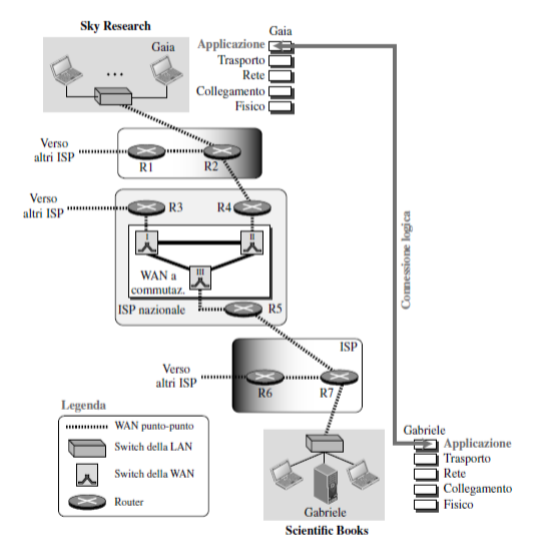
\includegraphics[scale=0.5]{assets/app_lvl.png}
	\end{center}
	Internet venne inizialmente progettata per fornire servizi ai suoi utenti. Alla sua nascita solo alcuni protocolli di livello applicazione erano disponibili per gli utenti. Oggi non è più possibile indicare il numero di protocolli esistenti poichè ne vengono costantemente aggiunti di nuovi grazie all'estrema flessibilità del livello applicazione.

	\section{Paradigmi del Livello Applicazione}
	Ormai è chiaro che per utilizzare Internet sono necessari due programmi che interagiscono tra loro: uno eseguito sul computer del mittente e l'altro sul computer del destinatario. I due programmi hanno la necessità di scambiarsi messsaggi sfruttando l'infrastruttura di Internet. Per fare ciò, bisogna stabilire delle modalità di relazione tra i due programmi. Queste modalità sono definite dai paradigmi del livello applicazione. I paradigmi più comuni sono:
	\begin{itemize}
		\item \textbf{Client-Server}: il paradigma tradizionale
		\item \textbf{Peer-to-Peer}: un paradigma più recente
		\item \textbf{Hybrid}: una combinazione dei due paradigmi precedenti
	\end{itemize}

	\section{Modello Client-Server}
	Nel modello \textit{client-server}, invece, esiste una chiara distinzione tra le entità che forniscono servizi (\textit{server}) e quelle che li consumano (\textit{client}). 
	Il server è attivo in maniera permanente, funge da nodo centrale e attende le richieste dai client e fornisce risorse, dati o servizi. I client sono programmi che vanno in esecuzione solo quando hanno bisogno di ottenere un servizio; iniziano la comunicazione inviando una richiesta delle risorse messe a disposizione dal server.
	\begin{center}
		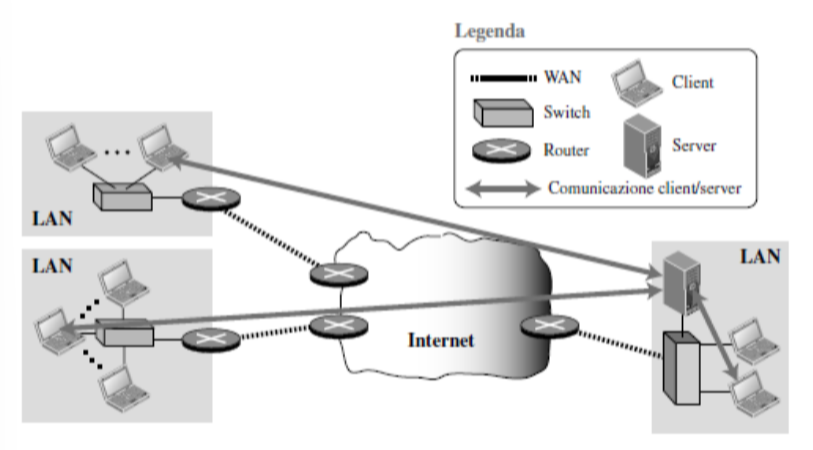
\includegraphics[scale=0.5]{assets/client-server.png}
	\end{center}

	\subsection{Vantaggi del Client-Server}
	Il modello client-server è particolarmente efficiente quando si tratta di amministrare grandi volumi di dati, poiché la gestione centralizzata permette di avere un controllo rigoroso su chi può accedere alle risorse e come queste vengono utilizzate. Inoltre, l'architettura centralizzata consente una più facile implementazione di politiche di sicurezza, backup e manutenzione, poiché tutte le risorse critiche risiedono sul server.

	\subsection{Svantaggi del Client-Server}
	Tuttavia, questa centralizzazione rappresenta anche un punto di vulnerabilità: se il server dovesse subire un'interruzione, tutti i client collegati perderebbero l'accesso ai servizi. Inoltre, man mano che il numero di client aumenta, il server potrebbe diventare un collo di bottiglia, richiedendo hardware più potente per gestire un numero crescente di richieste.

	\section{Tipologie di Ambiente Client-Server}
	All'interno dell'architettura client-server, esistono diverse tipologie di implementazioni basate sulla natura dei servizi forniti dal server. Le due principali sono:
	\begin{enumerate}
		\item \textbf{File Server}: Dove il server gestisce principalmente l'accesso ai file e funge da repository.
		\item \textbf{Application Server}: Dove il server non solo gestisce i file, ma esegue anche applicazioni che forniscono funzionalità avanzate ai client.
	\end{enumerate}

	\section{File Server}
	Nel caso di un \textit{file server}, il ruolo principale del server è quello di archiviare e gestire l'accesso ai file. L'applicazione stessa risiede ed è eseguita sui computer client, e il server agisce come un deposito di dati. 

	\paragraph{Esempio}
	Un esempio comune di configurazione file server è l'ambiente di redazione documenti in una rete LAN, dove ogni utente utilizza un programma di videoscrittura (word processor) installato localmente sul proprio computer. I documenti creati vengono salvati sul server, che funge da repository centrale per i dati, ma non esegue alcuna elaborazione legata all'applicazione stessa. In questo caso, le operazioni di calcolo e di elaborazione vengono svolte esclusivamente dal client.

	\subsection{Vantaggi del File Server}
	L'architettura file server è semplice da implementare e fornisce una separazione chiara tra applicazioni e dati. I dati, essendo centralizzati, sono più facili da gestire, e l'accesso può essere monitorato e controllato centralmente.

	\subsection{Svantaggi del File Server}
	Uno svantaggio di questa configurazione è che, in caso di accesso concorrente a grandi quantità di dati, le prestazioni della rete potrebbero degradare. Inoltre, il server funge solo da archivio, non contribuendo all'elaborazione dei dati, il che potrebbe limitare l'efficienza in scenari più complessi.

	\section{Application Server}
	Nel caso di un \textit{application server}, oltre alla gestione dei dati, il server esegue anche le applicazioni stesse. Questo modello è utilizzato in situazioni in cui l'applicazione client-server ha una parte client leggera che interagisce con un server che esegue le operazioni più complesse.

	\paragraph{Esempio}
	Un esempio tipico è un software gestionale aziendale basato su un database. Il client agisce solo come un'interfaccia che permette all'utente di formulare una query SQL, mentre l'application server esegue effettivamente la query sul database e restituisce i risultati. Questo approccio riduce il carico di lavoro sui client e centralizza le operazioni complesse sul server, che può essere dimensionato adeguatamente per gestire elevati volumi di richieste.

	\subsection{Vantaggi dell'Application Server}
	Il principale vantaggio di un application server è la capacità di eseguire applicazioni complesse sul server stesso, riducendo il carico sui client. Inoltre, le risorse computazionali possono essere ottimizzate sul server, garantendo una gestione efficiente delle applicazioni.

	\subsection{Svantaggi dell'Application Server}
	Tuttavia, come per il modello file server, la centralizzazione rappresenta un potenziale punto di fallimento. Se il server smette di funzionare o è sovraccarico, i client non possono eseguire le applicazioni, rendendo l'intera rete inaccessibile.

	Questi modelli si differenziano non solo per l'architettura, ma anche per l'approccio alla gestione delle risorse, alla distribuzione dei dati e alla sicurezza. Ciascuno di questi modelli è adatto a specifici casi d'uso e presenta vantaggi e svantaggi a seconda delle esigenze dell'utente e delle infrastrutture disponibili.

	\section{Modello Peer-to-Peer}
	Nel modello \textit{peer-to-peer} (P2P), tutti gli host sono paritetici, ovvero operano allo stesso livello nella rete. Non esiste un'entità centrale che controlla il flusso di dati o le risorse, e ogni nodo della rete può sia offrire servizi sia fruirne. Questo approccio si basa sulla decentralizzazione e sulla distribuzione delle risorse tra tutti i partecipanti alla rete.

	\begin{center}
		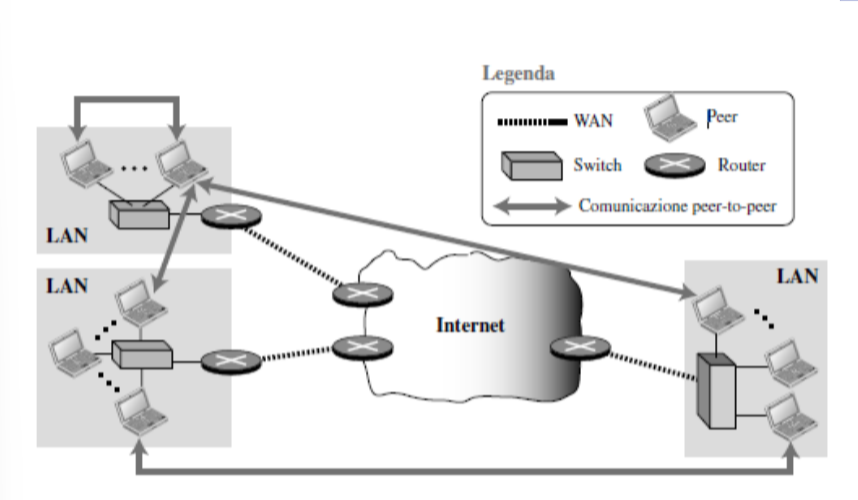
\includegraphics[scale=0.5]{assets/p2p.png}
	\end{center}

	\subsection{Vantaggi del Peer-to-Peer}
	Uno dei principali vantaggi del modello P2P è la scalabilità: poiché ogni nodo può contribuire sia come client che come server, la rete può crescere facilmente con l'aumentare del numero di partecipanti. Inoltre, non essendoci un singolo punto di controllo o di fallimento, la rete P2P è altamente resiliente e continua a funzionare anche se alcuni nodi si disconnettono.

	\subsection{Svantaggi del Peer-to-Peer}
	Tuttavia, la mancanza di una gestione centralizzata può portare a problemi di sicurezza e amministrazione. L'assenza di controllo centralizzato significa che è difficile applicare politiche di gestione e protezione dei dati, il che rende più vulnerabile la rete a intrusioni, attacchi o comportamenti non autorizzati. Inoltre, in molte reti P2P, le prestazioni possono variare notevolmente a seconda della partecipazione e della capacità dei nodi.

	\section{API - Application Programming Interface}
	Le API (\textit{Application Programming Interfaces}) sono insiemi di regole e strumenti che permettono a un programma di comunicare con un altro software o servizio. Quando si sviluppa un'applicazione che deve comunicare tramite rete, l'API gestisce l'interazione tra il programma e il sistema operativo, consentendo l'accesso ai primi quattro livelli dello stack TCP/IP per aprire connessioni, inviare e ricevere dati, e chiudere le connessioni.
	\vspace{\baselineskip}\\
	Nel contesto delle reti, l'API più utilizzata è la \textit{Socket Interface}, che fornisce le funzioni necessarie per gestire le connessioni di rete. Le socket permettono ai processi applicativi di comunicare attraverso la rete in maniera astratta, senza preoccuparsi dei dettagli tecnici di basso livello. Grazie a questa astrazione, i programmatori possono concentrarsi sulla logica dell'applicazione, lasciando che l'API gestisca la comunicazione di rete sottostante.
	\vspace{\baselineskip}\\
	Una \textbf{socket} è un'interfaccia di comunicazione tra due processi, che possono essere eseguiti sulla stessa macchina o su macchine diverse. Una socket è identificata da due elementi chiave:
	\begin{itemize}
		\item Un indirizzo IP, che identifica univocamente un dispositivo connesso a una rete.
		\item Un numero di porta, che specifica il processo in esecuzione su quel dispositivo.
	\end{itemize}
	\begin{center}
		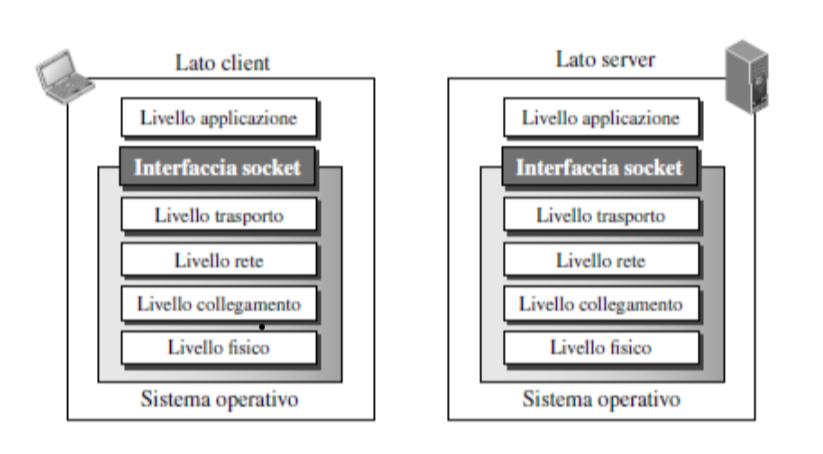
\includegraphics[scale=0.5]{assets/socket-int.png}	
	\end{center}
	Nel modello client-server, la comunicazione avviene tra una socket del client e una socket del server:
	\begin{itemize}
		\item Il client crea una socket e la utilizza per connettersi alla socket del server.
		\item Il server, dal canto suo, crea una socket e rimane in ascolto, pronto a gestire le connessioni in arrivo.
	\end{itemize}
	\begin{center}
		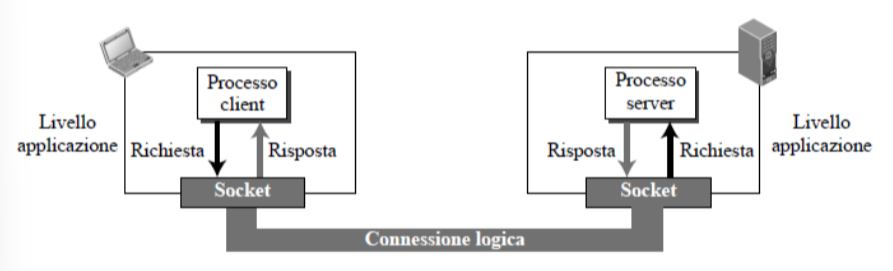
\includegraphics[scale=0.5]{assets/socket-comm.png}
	\end{center}
	Ogni comunicazione tra client e server richiede due indirizzi, chiamati \textbf{socket address}, uno per il mittente (locale) e uno per il destinatario (remoto). Un \textit{socket address} è composto da:
	\begin{itemize}
		\item L'indirizzo IP, che identifica l'host (la macchina connessa alla rete).
		\item Il numero di porta, che identifica il processo all'interno di quell'host.
	\end{itemize}
	Dal lato server, l'indirizzo IP è generalmente fisso e fornito dal sistema operativo, mentre la porta può essere predefinita (well-known) per servizi standard o assegnata dinamicamente per processi non standard. Dal lato client, il sistema operativo assegna un \textbf{socket address locale} univoco durante la comunicazione, scegliendo un numero di porta temporaneo (detto \textbf{porta effimera}) per garantire che non vi siano conflitti con altre connessioni attive.
	\vspace{\baselineskip}\\
	Se il client si connette a un server noto, il \textbf{socket address remoto} (IP e porta del server) è noto fin dall'inizio. Tuttavia, se il client si connette a un server di cui conosce solo il nome di dominio, l'indirizzo IP del server viene risolto tramite il \textbf{DNS} (\textit{Domain Name System}), un servizio che traduce i nomi di dominio in indirizzi IP.
	\vspace{\baselineskip}\\
	Una coppia di processi fornisce servizi agli utenti di Internet, siano questi persone o applicazioni. La coppia di processi, tuttavia, deve utilizzare i servizi offerti dal livello trasporto per la comunicazine, poichè non vi è comunicazione fisica a livello applicazione.
	\vspace{\baselineskip}\\
	Nel livello trasporto dello stack TCP/IP, due protocolli principali sono utilizzati per la comunicazione tra processi:
	\begin{itemize}
		\item \textbf{TCP} (\textit{Transmission Control Protocol}): Un protocollo affidabile e orientato alla connessione, che garantisce l'invio dei dati nell'ordine corretto e la ritrasmissione in caso di errore. Questo è utilizzato per applicazioni che richiedono affidabilità, come il trasferimento di file e le comunicazioni web.
		\item \textbf{UDP} (\textit{User Datagram Protocol}): Un protocollo non orientato alla connessione, più veloce ma meno affidabile, poiché non garantisce l'ordine dei dati né la loro ritrasmissione in caso di perdita. È ideale per applicazioni che richiedono velocità, come lo streaming video o le chiamate VoIP.
	\end{itemize}
	\begin{center}
		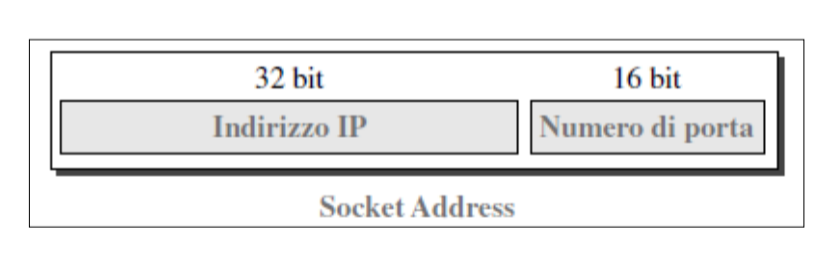
\includegraphics[scale=0.5]{assets/socket-addr.png}
	\end{center}

	\section{Applicazioni Client/Server Standard}
	\subsection{WWW}
	La \textbf{World Wide Web} (WWW) è una architettura distribuita di informazioni basata su ipertesti che consente di accedere e visualizzare contenuti multimediali attraverso Internet. Il WWW è costituito da pagine web, che possono contenere testo, immagini, video, audio e collegamenti ipertestuali a altre pagine web. Per accedere alle pagine web, è necessario utilizzare un \textbf{web browser}, un'applicazione che consente di visualizzare e interagire con i contenuti web. E' possibile accedere alle pagine web tramite un \textbf{URL} (\textit{Uniform Resource Locator}), un indirizzo che identifica univocamente una risorsa su Internet.

	\subsection{HTTP}
	Il \textbf{protocollo HTTP} (\textit{HyperText Transfer Protocol}) è il protocollo di comunicazione utilizzato per trasferire le pagine web da un server web a un client web. Il protocollo HTTP è basato su una struttura client-server, in cui il client (il browser web) invia una richiesta al server web per ottenere una pagina web utilizzando un numero di porta effimero, e il server invia la pagina richiesta al client utlizzando il numero di porta 80.  Sfrutta, inoltre, il protocollo TCP per garantire l'affidabilità e l'ordine dei dati. Il protocollo HTTP è stato progettato per essere semplice e flessibile, consentendo di trasferire non solo pagine web, ma anche immagini, video, audio e altri tipi di contenuti multimediali.
	Stabilisce, quindi, se la connessione deve essere persistente o meno, come devono essere strutturati i messaggi e come devono essere effettuate richieste condizionali, come devono essere memorizzati i dati e come devono essere gestiti i cookie.

	\subsubsection{Web Caching}
	Per ridurre il tempo di caricamento delle pagine web e il traffico di rete, i browser web e i server web utilizzano il \textbf{web caching}, una tecnica che memorizza temporaneamente le pagine web e i file multimediali sul disco rigido del client o del server. Quando un client richiede una pagina web, il browser verifica se la pagina è già presente nella cache locale. Se la pagina è presente e non è scaduta, il browser carica la pagina dalla cache locale anziché richiederla al server web, riducendo la latenza, il carico sul server originale e il traffico di rete. 
	\vspace{\baselineskip}\\
	Una delle soluzioni più comuni per il web caching è l'utilizzo di \textbf{proxy server}, server intermedi che memorizzano le pagine web richieste dai client e le forniscono ai client successivi senza doverle richiedere nuovamente al server web. Il server proxy agisce da server quando ha una risposta pronta per il client, mentre agisce da client quando non ha la risposta e deve inoltrare la richiesta al server web. Il server proxy viene solitamente collocato in prossimità dei client, quindi o nel client stesso, oppure nella stessa LAN del client, o in certi casi un ISP con numerosi utenti può installare un proxy per ridurre il carico in entrata e uscita alla propria rete.
	\begin{center}
		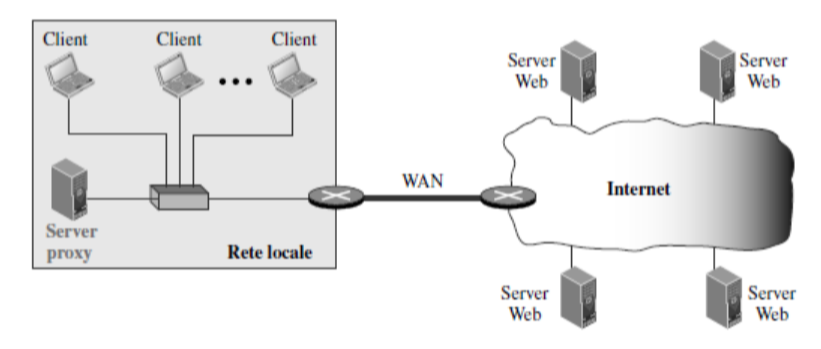
\includegraphics[scale=0.5]{assets/proxy-pos.png}
	\end{center}
	Un server proxy può essere utilizzato anche per altri scopi:
	\begin{itemize}
		\item \textbf{Filtraggio dei contenuti}: bloccare l'accesso a determinati siti web o tipi di contenuti. Questo aspetto può essere utile come strumento di censura.
		\item \textbf{Controllo degli accessi}: limitare l'accesso a Internet a determinati orari o a determinati utenti.
		\item \textbf{Accesso all'esterno}: consentire ad una rete privata di accedere a Internet e immagazzinare i risultati delle richieste di un utente in modo tale da ridurre il tempo di risposta nel caso in cui un altro utente effettui la stessa richiesta.
		\item \textbf{Tracciamento}: tenere traccia delle operazioni effettuate come pagine web visitate, file scaricati e dati inviati, offrendo statistiche ed osservazioni dell'utilizzo della rete, tali da violare la privacy degli utenti. 
		\item \textbf{Sicurezza}: consentire ad una rete privata di accedere a Internet attraverso un unico indirizzo IP pubblico, nascondendo gli indirizzi IP reali dei client e proteggendo la rete interna da attacchi esterni. Questo tipo di server proxy è noto come \textbf{proxy server inverso}.
	\end{itemize} 

	\subsubsection{Browser}
	Il \textbf{browser} è un'applicazione software che consente di visualizzare e interagire con le pagine web. I browser web supportano diverse tecnologie e standard, come HTML, CSS, JavaScript e Flash, che consentono di visualizzare e interagire con i contenuti web. I browser web più comuni includono Google Chrome, Mozilla Firefox, Microsoft Edge, Safari e Opera. Esso è composto da tre componenti:
	\begin{itemize}
		\item controllore: gestisce l'interfaccia utente e le interazioni con l'utente.
		\item modulo di protocollo client: gestisce la comunicazione con i server web utilizzando il protocollo HTTP o FTP.
		\item interpreti: interpretano e visualizzano i contenuti web, come HTML, CSS e JavaScript.
	\end{itemize}
	\begin{center}
		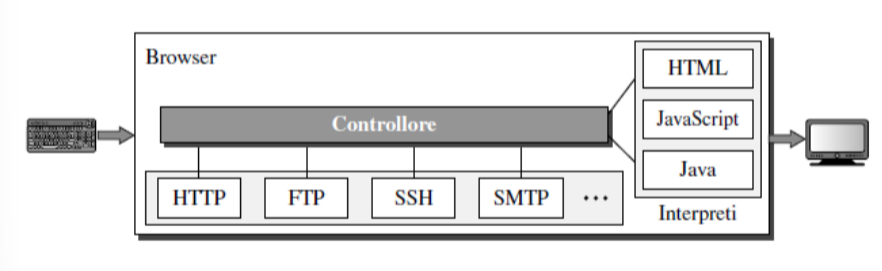
\includegraphics[scale=0.5]{assets/browser.png}
	\end{center}
	Il conotrollore riceve l'input da tastiera o mouse, comunica con il modulo di protocollo client per inviare richieste HTTP ai server web, riceve le risposte dai server web e passa i contenuti web agli interpreti per la visualizzazione.

	\subsubsection{URL - Uniform Resource Locator}
	L'URL (\textit{Uniform Resource Locator}) è un indirizzo che identifica univocamente una risorsa su Internet. Un URL è composto da diversi elementi:
	\begin{itemize}
		\item \textbf{Schema}: specifica il protocollo utilizzato per accedere alla risorsa, come HTTP, HTTPS, FTP o file.
		\item \textbf{Host}: specifica il nome di dominio o l'indirizzo IP del server che ospita la risorsa.
		\item \textbf{Porta}: specifica la porta di rete utilizzata per la comunicazione con il server. La porta predefinita per HTTP è la 80.
		\item \textbf{Percorso}: specifica il percorso della risorsa sul server, come il nome del file o della directory.
		\item \textbf{Query}: specifica i parametri aggiuntivi per la richiesta, come i dati di ricerca o le opzioni di visualizzazione.
		\item \textbf{Frammento}: specifica una parte specifica della risorsa, come un'ancora o un'etichetta.
	\end{itemize}
	\begin{center}
		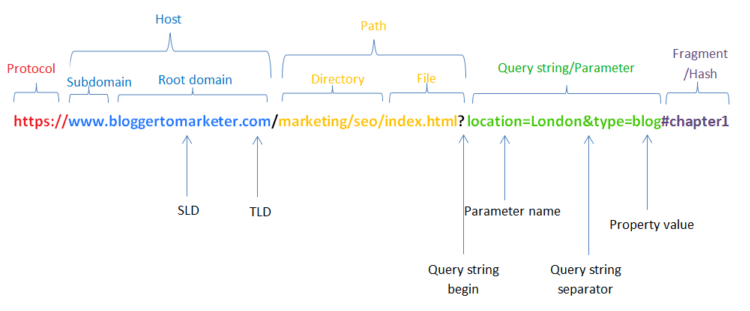
\includegraphics[scale=0.5]{assets/url.png}
	\end{center}

	\subsubsection{Documenti Web}
	I documenti web sono file di testo formattati in HTML (\textit{HyperText Markup Language}) che contengono testo, immagini, collegamenti ipertestuali e altri elementi multimediali. Essi possono essere statici, dinamici o attivi. I documenti web statici sono file HTML (o XHTML) che vengono memorizzati su un server web e inviati ai client senza alcuna elaborazione. I documenti web dinamici, d'altra parte, sono generati dinamicamente da un'applicazione web o da un server web utilizzando dati provenienti da un database o da altre fonti. Infine, i documenti web attivi contengono script o codice eseguibile che consente di interagire con l'utente o di modificare il contenuto della pagina in tempo reale.

	\subsubsection{Connessioni Persistenti e Non Persistenti}
	La connessione persistente usa sempre la stessa connessione TCP per trasferire più file, mentre la connessione non persistente apre una nuova connessione TCP per ogni file. Le connessioni non persistenti sono meno utilizzate poichè causano sovraccarico sul server che deve usare un buffer diverso per ogni connessione aperta. Nelle connessioni persistenti la connessione rimane aperta in attesa di ulteriori richieste finchè il server non chiude la connessione su richiesta del client o allo scadere del timeout. In questo modo si risparmiano tempo e risorse.
	\newpage
	\paragraph{Esempio di Connessione Non Persistenti}
	\begin{center}
		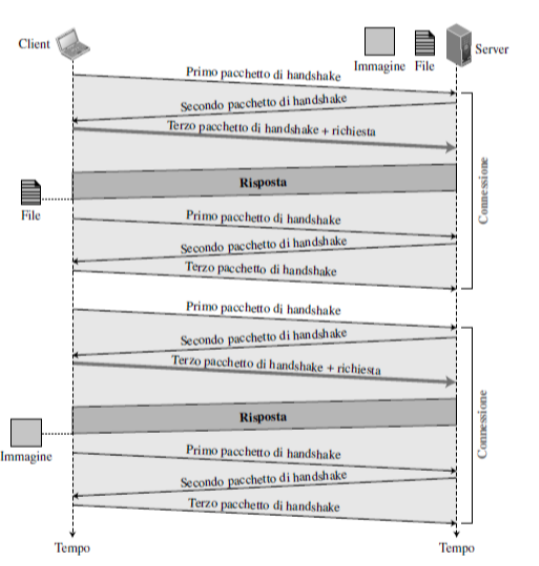
\includegraphics[scale=0.5]{assets/non-persistent.png}
	\end{center}

	\paragraph{Esempio di Connessione Persistenti}
	\begin{center}
		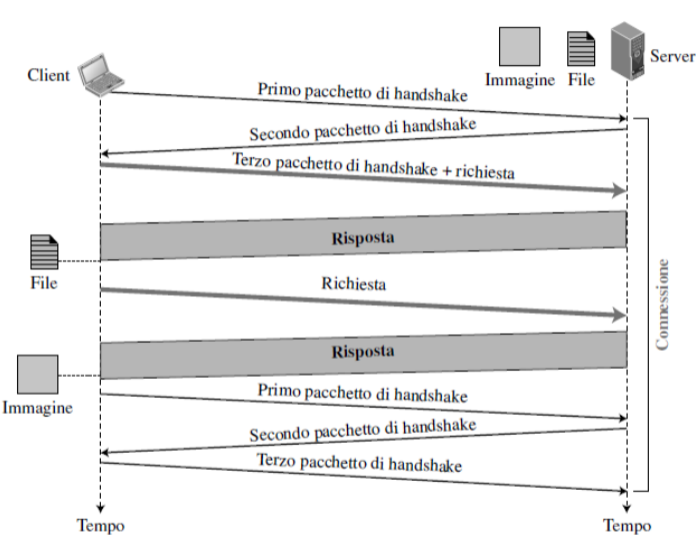
\includegraphics[scale=0.5]{assets/persistent.png}
	\end{center}
	
	\subsubsection{Formato dei messaggi di richiesta e risposta HTTP}
	\begin{center}
		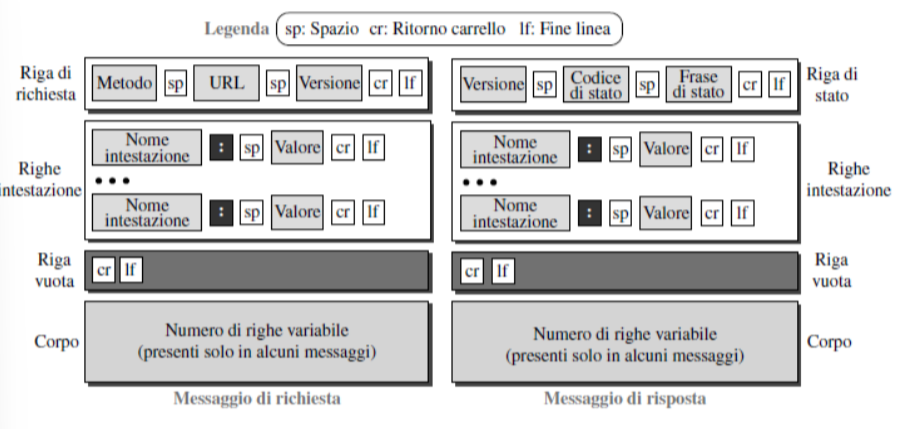
\includegraphics[scale=0.5]{assets/http-msg.png}
	\end{center}

	\subsubsection{Metodi HTTP}
	Il protocollo HTTP definisce diversi metodi che specificano l'azione da eseguire sul server web. I metodi HTTP più comuni sono:
	\begin{itemize}
		\item \textbf{GET}: richiede un documento dal server. I dati vengono trasmessi direttamente nell'URL.
		\item \textbf{HEAD}: richiede le informazioni relative a un documento, ma non il documento stesso.
		\item \textbf{POST}: invia dati al server per essere elaborati. I dati vengono trasmessi nel corpo della richiesta.
		\item \textbf{PUT}: carica un documento sul server.
		\item \textbf{DELETE}: elimina un documento dal server.
		\item \textbf{OPTIONS}: restituisce le opzioni di comunicazione per il server.
		\item \textbf{TRACE}: restituisce una copia della richiesta ricevuta dal server.
		\item \textbf{CONNECT}: converte la richiesta in un tunnel TCP/IP. E' un metodo riservato.
	\end{itemize}

	\subsubsection{Header di una richiesta HTTP}
	Una richiesta HTTP è composta da due parti: l'\textbf{header} e il \textbf{body}. L'header contiene informazioni sul client, sul server e sulla richiesta stessa. Alcuni campi comuni dell'header di una richiesta HTTP sono:
	\begin{itemize}
		\item \textbf{Host}: specifica il dominio/l'IP e la porta del client.
		\item \textbf{User-Agent}: specifica il browser o l'applicazione client utilizzata per inviare la richiesta.
		\item \textbf{Accept}: specifica i tipi di contenuto accettati dal client.
		\item \textbf{Accept-language}: specifica le lingue accettate dal client.
		\item \textbf{Accept-encoding}: specifica i metodi di codifica accettati dal client.
		\item \textbf{Accept-charset}: specifica i set di caratteri accettati dal client.
		\item \textbf{Authorization}: specifica le credenziali di autenticazione del client.
		\item \textbf{Date}: specifica la data e l'ora della richiesta.
		\item \textbf{Upgrade}: specifica i protocolli di comunicazione preferito.
		\item \textbf{Cookie}: specifica i cookie inviati dal client al server.
		\item \textbf{If-Modified-Since}: invia il documento al client solo se è stato modificato dopo la data specificata.
	\end{itemize}

	\subsubsection{Header e messaggio di risposta HTTP}
	Una risposta HTTP è composta da due parti: l'\textbf{header} e il \textbf{body}. L'header contiene informazioni sul server, sul client e sulla risposta stessa. Inoltre la risposta ha un campo di stato, che indica se la richiesta è stata elaborata correttamente o se si è verificato un errore. Gli status code si dividono nei seguenti intervalli:
	\begin{itemize}
		\item \textbf{1xx}: Informazioni
		\item \textbf{2xx}: Successo
		\item \textbf{3xx}: Redirezione
		\item \textbf{4xx}: Errore del client
		\item \textbf{5xx}: Errore del server
	\end{itemize}
	Alcuni campi comuni dell'header di una risposta HTTP sono:
	\begin{itemize}
		\item \textbf{Date}: specifica la data e l'ora della risposta.
		\item \textbf{Server}: specifica il software del server web utilizzato per generare la risposta.
		\item \textbf{Upgrade}: specifica i protocolli di comunicazione preferiti dal server.
		\item \textbf{Set-Cookie}: il server richiede al client di memorizzare un cookie.
		\item \textbf{Content-Type}: specifica il tipo di contenuto della risposta.
		\item \textbf{Content-Length}: specifica la lunghezza del corpo della risposta.
		\item \textbf{Content-Encoding}: specifica il metodo di codifica del corpo della risposta.
		\item \textbf{Content-Language}: specifica la lingua del corpo della risposta.
		\item \textbf{Location}: specifica l'URL a cui il client deve essere reindirizzato.
		\item \textbf{Last-Modified}: specifica la data e l'ora dell'ultima modifica del documento.
	\end{itemize}

	\paragraph{Esempio di richiesta e risposta HTTP}
	\begin{center}
		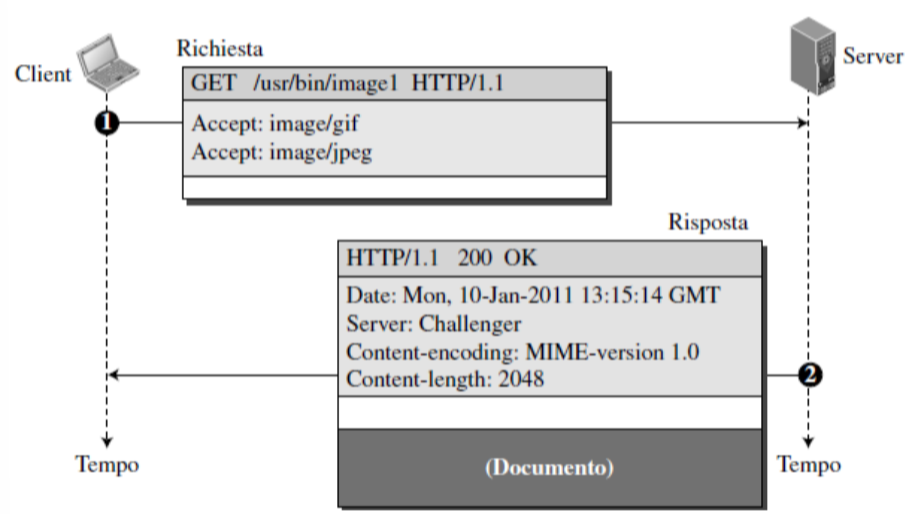
\includegraphics[scale=0.5]{assets/http-req-res.png}
	\end{center}
	\begin{center}
		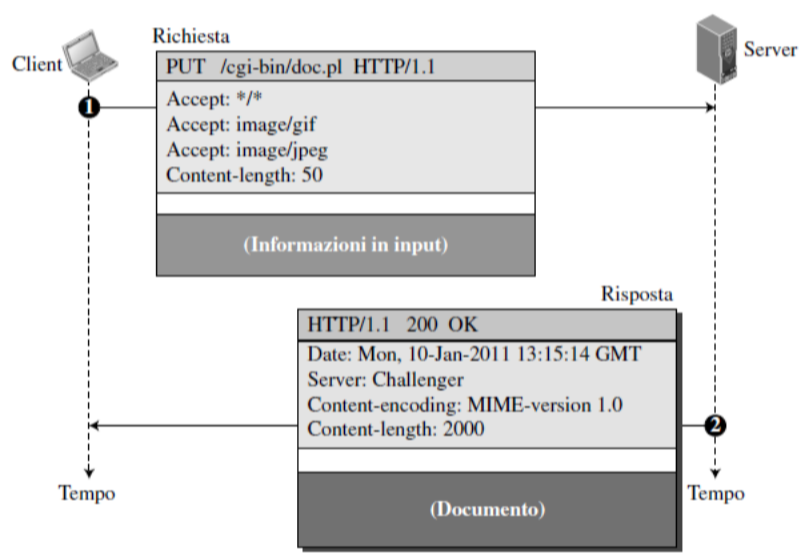
\includegraphics[scale=0.5]{assets/http-req-res2.png}
	\end{center}

	\subsubsection{Cookie}
	Inizialmente, il web si basava su protocolli senza stato, in cui ogni richiesta era indipendente dalle altre e non veniva mantenuta alcuna traccia dello stato del client. Tuttavia, questa mancanza di stato rendeva difficile la gestione delle sessioni utente e l'implementazione di funzionalità e applicazioni avanzate come gli e-commerce, le aree riservate o i servizi personalizzati. Per risolvere questo problema, sono stati introdotti i \textbf{cookie}, piccoli file di testo memorizzati sul computer del client che consentono ai siti web di memorizzare informazioni sulle preferenze e sullo stato del client. I cookie vengono inviati dal server al client tramite l'header HTTP \textit{Set-Cookie}. I cookie possono contribuire a migliorare l'esperienza dell'utente, consentendo ai siti web di memorizzare informazioni come le preferenze dell'utente, le impostazioni personalizzate, i dati di accesso e lo stato della sessione, evitanto all'utente di dover reinserire le stesse informazioni ogni volta che visita il sito. 
	\vspace{\baselineskip}\\
	Quando un client visita un sito web, il server crea un cookie memorizzando il nome del dominio del client, i contenuti di un cookie precedente, la data e l'ora di creazione e la data di scadenza, ecc. I cookie vengono memorizzati sul computer del client in un file di testo posizionato in un path diverso per ogni dominio del server. Quando un client visita nuovamente il sito web, il browser invia i cookie memorizzati, se presenti, al server, consentendo al server di recuperare le informazioni memorizzate e personalizzare l'esperienza dell'utente. Il cookie è creato e utilizzato dal server, ma memorizzato sul computer del client.
	\begin{center}
		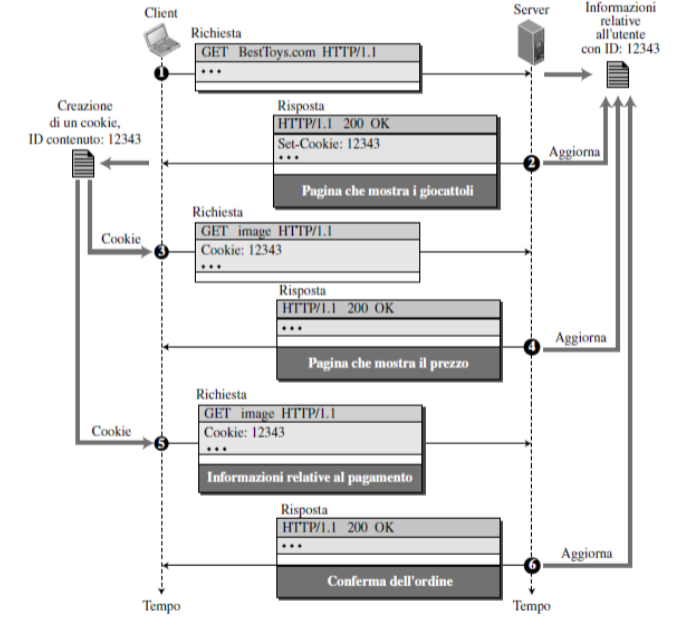
\includegraphics[scale=0.5]{assets/cookie.png}	
	\end{center}

	\subsubsection{Hosting e Housing}
	Realizzare un sito web significa progettare ed implementare un insieme di contenuti testuali e multimediali organizzati in forma ipertestuale. I “content” sono file digitali memorizzati su un disco che devono essere raggiungibili in ogni momento. Per ospitare tali file su un computer server è prassi che ci si rivolga ai servizi forniti da imprese specializzate (provider). Tale prassi si basa essenzialmente su motivi economici in quanto avere un proprio server funzionate 24h 365 giorni l’anno online richiede risorse finanziare e tecniche che molte aziende non possono permettersi. Un server ha infatti bisogno di energia elettrica stabile e senza interruzioni, di una temperatura controllata e costante, di connettività a banda larga, sicura ed affidabile. L’infrastruttura dovrebbe essere, inoltre, ridondata per garantire la massima affidabilità anche in caso di malfunzionamento. La fornitura di servizi di connessione ad Internet è così diventato un settore economico in cui operano molti provider che forniscono servizi molto diversi tra loro che si possono classificare come segue:
	\begin{itemize}
		\item \textbf{Housing}
		\item \textbf{Hosting}
		\item \textbf{VM}
	\end{itemize}

	\subsubsection{Hosting}
	L’\textbf{hosting} è un servizio con cui un sito web viene ospitato all’interno di un
	server di proprietà dell’Hosting Provider il quale è condiviso da più siti web di persone e/o aziende diverse. In pratica con un contratto di
	hosting un’azienda chiede il noleggio di una porzione di spazio del disco, una directory, di un server condividendone con altri affittuari le risorse. Essendo un servizio che presta hardware condiviso, potrebbe presentare delle criticità dal punto di vista della sicurezza. 

	\subsubsection{Housing}
	Con l’housing, invece, un’azienda “porta il proprio server” nella webfarm del provider. Il server sarà così ospitato all’interno di appositi armadi detti rack e può essere fornito direttamente dal cliente o anche acquistato presso il provider/hoster. L’hoster non avrà mai accesso al server del cliente, nè a livello fisico nè a livello software. Il server sarà gestito sempre con controllo remoto dall’azienda proprietaria. L’unico intervento che l’hoster è tenuto a fare è il riavvio fisico del server stesso. L’hosting è la soluzione migliore per quelle aziende che vogliano avere una presenza sul Web pur avendo un budget limitato e poca competenza tecnica per quanto riguarda la gestione del server. Per siti web con poco traffico giornaliero l’hosting è sicuramente la soluzione migliore. Di contro l’housing è utile quando si vuole un server di proprietà e l’azienda dispone di competenze tecniche. Ovviamente l’housing fornisce una flessibilità nell’installazione di software e nella gestione dei server che l’hosting non può fornire in quanto, in quest’ultimo caso, tutto è demandato all’hoster.

	\subsubsection{VM - Virtual Machine}
	Una \textbf{Virtual Machine} è un software che emula un computer reale e consente di eseguire più sistemi operativi su un singolo server fisico. Le VM sono utilizzate per consolidare i server fisici, ridurre i costi di gestione e manutenzione, e migliorare l'efficienza e la flessibilità delle risorse. Le VM possono essere create, gestite e distribuite in modo dinamico, consentendo di adattare le risorse in base alle esigenze dell'utente. Le VM sono utilizzate in ambienti di sviluppo e test, per la virtualizzazione dei server, per la migrazione dei carichi di lavoro e per la creazione di ambienti di sviluppo e test isolati. E' una soluzione flessibile e scalabile che consente di ridurre i costi e migliorare l'efficienza delle risorse. Si posiziona a metà fra l'hosting e l'housing poichè permette di avere un server virtuale condiviso con altri utenti, ma con risorse dedicate e garantite.

	\subsection{FTP - File Transfer Protocol}
	Il \textbf{File Transfer Protocol} (FTP) è un protocollo di rete utilizzato per trasferire file tra un client e un server. Il protocollo FTP è basato su una struttura client-server, in cui il client invia comandi al server per trasferire file, creare directory, eliminare file e altre operazioni di gestione dei file. Il protocollo FTP utilizza due connessioni separate per trasferire i file: una connessione di controllo per inviare comandi e ricevere risposte, e una connessione dati per trasferire i file effettivi. Sebbene il trasferimento di un file possa sembrare un'operazione semplice, vi sono numerosi problemi ai quali bisogna prestare attenzione: i due sistemi coinvolti possono adottare convenzioni differenti per la denominazione dei file oppure gestire in modo differente la struttura delle directory. Questi problemi vengono risolti dal protocollo FTP.

	\begin{center}
		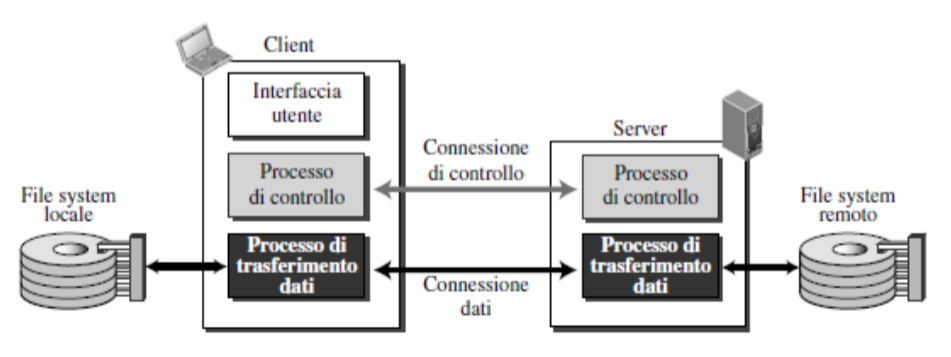
\includegraphics[scale=0.5]{assets/ftp.png}
	\end{center}

	\subsubsection{Client FTP}
	Un \textbf{client FTP} è un'applicazione software che consente di trasferire file tra un computer locale e un server remoto utilizzando il protocollo FTP e gestisce i processi di controllo e trasferimento. I client FTP forniscono un'interfaccia utente intuitiva per caricare, scaricare, rinominare, eliminare e gestire i file sul server remoto. Alcuni client FTP supportano anche funzionalità avanzate come la sincronizzazione dei file, la crittografia dei dati e la gestione delle connessioni multiple. Alcuni client FTP popolari includono FileZilla, Cyberduck, WinSCP e CuteFTP.

	\subsubsection{Server FTP}
	Un \textbf{server FTP} è un sistema progettato per gestire il trasferimento di file attraverso la rete. Funziona come un deposito centralizzato dove i file possono essere archiviati e accessibili da vari client. Quando un utente desidera scaricare o caricare un file, il client FTP invia una richiesta al server, il quale verifica le credenziali dell'utente per garantire che abbia il permesso di accedere alle risorse richieste. Una volta autenticato, il server permette all'utente di navigare tra le directory e di interagire con i file, gestendo operazioni come il download e l'upload. Può anche organizzare i file in una struttura gerarchica, facilitando la ricerca e la gestione. Inoltre, il server FTP può essere configurato per offrire diversi livelli di accesso, come accesso anonimo o autenticato, a seconda delle necessità. Questo consente di mantenere la sicurezza dei dati, limitando l'accesso a file sensibili solo agli utenti autorizzati. In sintesi, il server FTP è un elemento cruciale per il trasferimento sicuro ed efficiente dei file su una rete.

	\subsubsection{Durata delle connessioni}
	Le connessioni FTP possono essere di due tipi: di controllo e di dati. La connessione di controllo è utilizzata per inviare comandi e ricevere risposte tra il client e il server e rimane aperta per tutta la durata della sessione FTP. La connessione di dati, d'altra parte, è utilizzata per trasferire i file effettivi e viene aperta solo quando è necessario trasferire i dati. Una volta completato il trasferimento, la connessione di dati viene chiusa. La connessione di controllo utilizza la porta 21, mentre la connessione di dati può utilizzare una porta casuale o la porta 20.

	\subsubsection{Comandi FTP}
	\begin{center}
		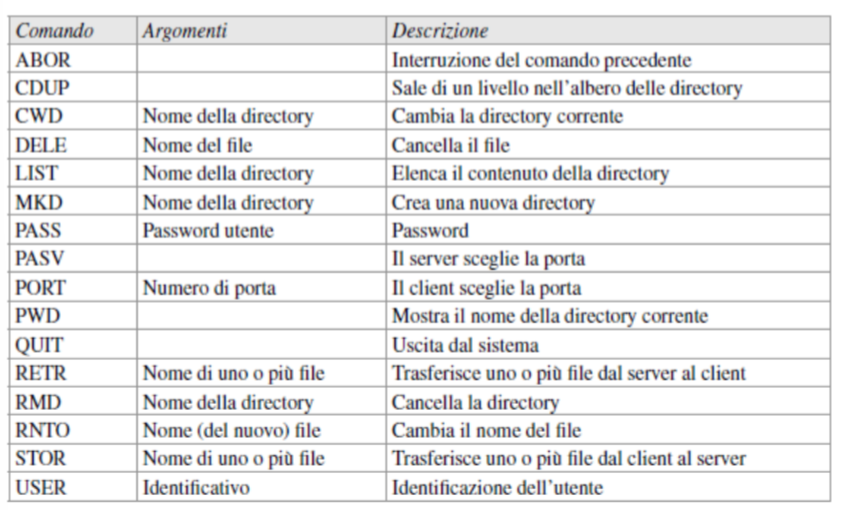
\includegraphics[scale=0.6]{assets/ftp-cmd.png}
	\end{center}

	\subsubsection{Risposte FTP}
	\begin{center}
		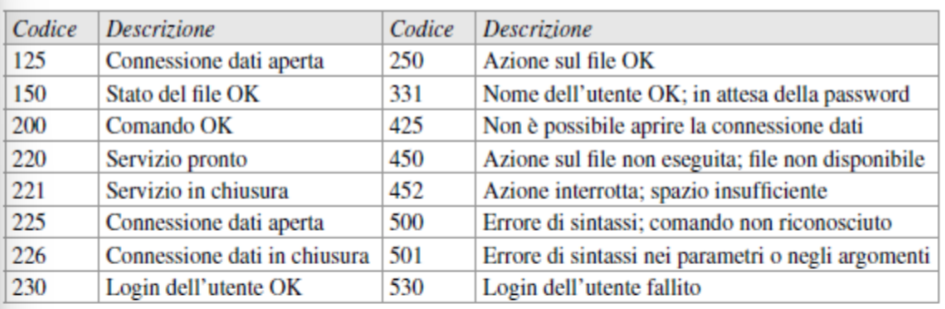
\includegraphics[scale=0.6]{assets/ftp-res.png}
	\end{center}

	\paragraph{Eesempio di connessione FTP}
	\begin{center}
		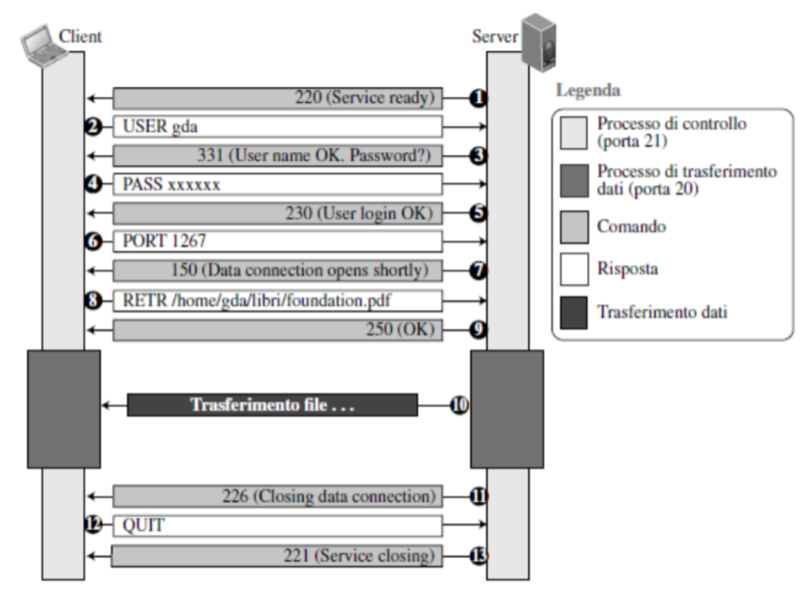
\includegraphics[scale=0.5]{assets/ftp-ex.png}
	\end{center}

	\subsection{Posta elettronica}
	La \textbf{posta elettronica} (e-mail) è un servizio di comunicazione che consente di inviare e ricevere messaggi elettronici attraverso Internet. L'e-mail è uno dei servizi più utilizzati su Internet, poiché consente di inviare messaggi in modo rapido, economico e affidabile. Al contrario di HTTP e FTP nei quali il programma server è sempre in esecuzione in attesa di una richiesta dal client, nella posta elettronica la comunicazione è unidirezionale. Questo servizio è basato su due pilastri:
	\begin{itemize}
		\item \textbf{MTA - Message Transfer Agent}: ossia il protocollo SMTP, che si occupa di trasferire i messaggi tra i server di posta elettronica gestendo la consegna di un messaggio, i comandi e le risposte ai comandi.
		\item \textbf{MAA - Message Access Agent}: che può essere uno tra i protocolli POP3 e IMAP e hanno il compito di permettere ai client di accedere alle caselle di posta elettronica conservando i messaggi.
	\end{itemize}
	\begin{center}
		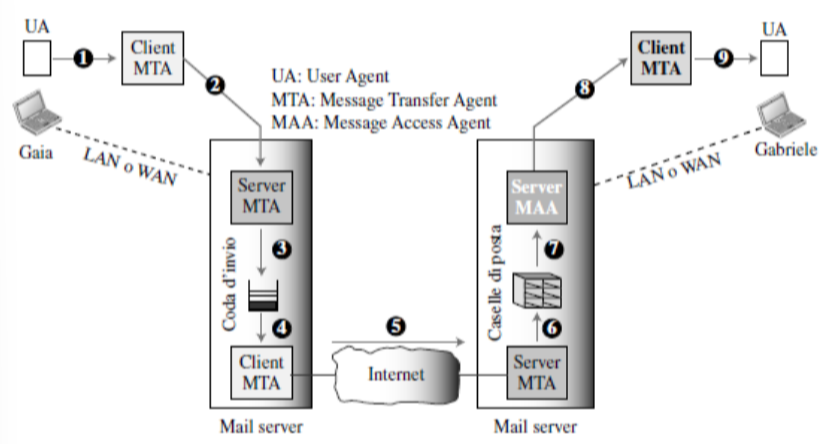
\includegraphics[scale=0.5]{assets/email.png}
	\end{center}
	\begin{center}
		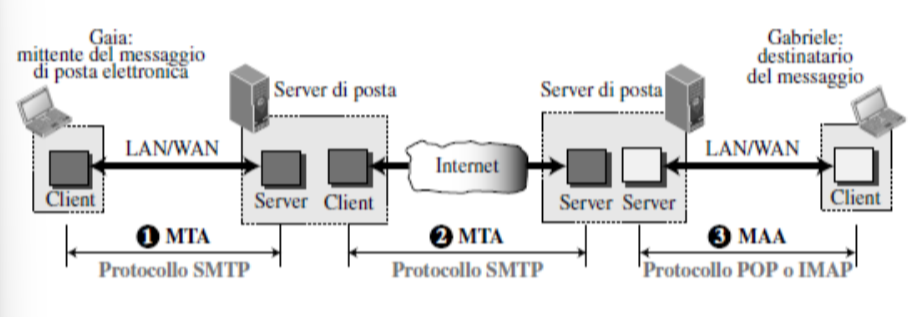
\includegraphics[scale=0.5]{assets/email-comm.png}
	\end{center}
	Gli indirizzi email sono composti da due parti: il nome utente e il dominio. Il nome utente identifica l'utente specifico, mentre il dominio identifica il server di posta elettronica che gestisce l'account dell'utente. Gli indirizzi email sono univoci e non possono essere duplicati. 
	\vspace{\baselineskip}\\
	I comandi del protocollo SMTP sono:
	\begin{itemize}
		\item \textbf{HELO nome-host-mittente}: l'host mittente si identifica
		\item \textbf{MAIL FROM mittente-messaggio}: specifica l'indirizzo email del mittente.
		\item \textbf{RCPT TO destinatario}: specifica l'indirizzo email del destinatario.
		\item \textbf{DATA corpo-messaggio}: invia il messaggio email.
		\item \textbf{QUIT}: chiude la connessione SMTP.
		\item \textbf{RSET}: annulla la transazione corrente.
		\item \textbf{VRFY nome-destinatario}: verifica la validità dell'indirizzo del destinatario-
	\end{itemize}
	Le principali risposte del protocollo SMTP sono:
	\begin{itemize}
		\item \textbf{220}: il server è pronto.
		\item \textbf{221}: il server è in procinto di chiudere la connessione.
		\item \textbf{250}: richiesta accettata.
		\item \textbf{251}: l'utente non è locale al mail server, il messaggio verrà inoltrato.
		\item \textbf{354}: è effettuabile l'invio del messaggio
		\item \textbf{421}: servizio non disponibile.
		\item \textbf{450}: errore temporaneo, mailbox non disponibile.
		\item \textbf{451}: errore locale. comando interrotto.
		\item \textbf{452}: memoria non sufficiente, comando interrotto.
		\item \textbf{500}: comando non riconosciuto.
		\item \textbf{501}: errore di sintassi nei parametri o argomenti.
		\item \textbf{502}: comando non disponibile.
		\item \textbf{503}: sequenza di comandi errata.
		\item \textbf{550}: mailbox non disponibile, comando non eseguito.
		\item \textbf{551}: l'utente non è locale al mail server.
		\item \textbf{552}: spazio insufficiente, comando non eseguito.
		\item \textbf{554}: transazione fallita.
	\end{itemize}
	La comunicazione di posta elettronica parte con l'apertura della connessione dopo che il server SMTP approva in seguito alla connessione TCP del client sulla porta 25. Successivamente avviene il trasfermento del messaggio ad uno o più destinatari. A invio completato, il client chiude la connessione con il server.
	\begin{center}
		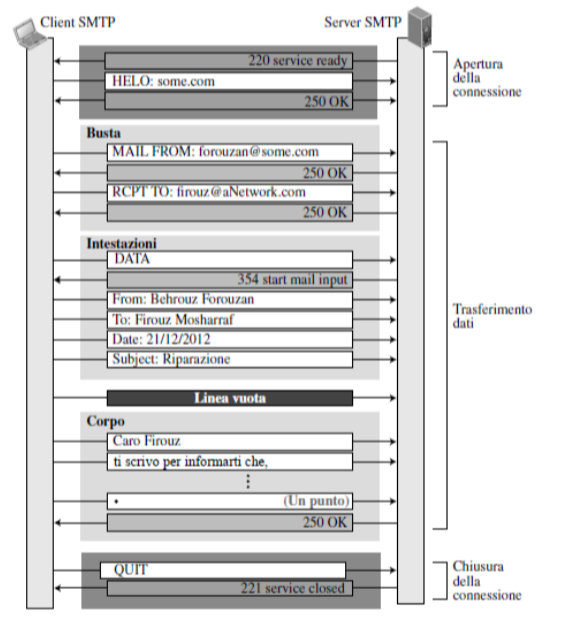
\includegraphics[scale=0.5]{assets/email-comm2.png}
	\end{center}
	Il protocollo SMTP si occupa dell'invio del messaggio dal client al server, mentre il protocollo POP3 o IMAP si occupa del recupero del messaggio dal server al client. Il protocollo POP3 scarica il messaggio dal server e lo elimina dal server, mentre il protocollo IMAP sincronizza il messaggio tra il server e il client, consentendo di visualizzare e gestire i messaggi su più dispositivi.
	Un'alternativa è il protocollo MIME (\textit{Multipurpose Internet Mail Extensions}), che consente di inviare messaggi di posta elettronica con contenuti multimediali come immagini, audio e video. Il protocollo MIME estende il protocollo SMTP per supportare i contenuti multimediali e i tipi di file non testuali. I principali tipi di file supportati da MIME sono:
	\begin{itemize}
		\item \textbf{Text}: 
		\begin{itemize}
			\item \textbf{Plain}: testo semplice.
			\item \textbf{HTML}: testo formattato in HTML.
		\end{itemize}
		\item \textbf{Multipart}:
		\begin{itemize}
			\item \textbf{Mixed}: corpo composto da una lista ordinata di parti con formati diversi.
			\item \textbf{Parallel}: come il precedente ma le diverse parti non sono ordinate.
			\item \textbf{Alternative}: parti sono versioni differenti dello stesso contenuto.
		\end{itemize}
		\item \textbf{Message}:
		\begin{itemize}
			\item \textbf{RFC822}: messaggio incapsulato.
			\item \textbf{Partial}: frammento di un messaggio più grande.
			\item \textbf{External-body}: riferimento di un altro messaggio
		\end{itemize}
		\item \textbf{Image}: immagini come JPEG, PNG e GIF.
		\item \textbf{Audio}: file audio come MP3 e WAV.
		\item \textbf{Video}: file video come MP4, MPEG e AVI.
		\item \textbf{Application}: file binari come PDF, ZIP e EXE.
	\end{itemize}
	Questi file possono essere encodati in 7 bit, 8 bit, binario, base64 o quoted-printable per garantire la compatibilità con i diversi client di posta elettronica.

	\subsection{Telnet - Terminal Network}
	Il \textbf{Telnet} è un protocollo di rete utilizzato per stabilire una connessione remota tra un client e un server. Il protocollo Telnet consente di accedere e controllare un computer remoto tramite una connessione di rete, consentendo di eseguire comandi e interagire con il sistema remoto come se ci si trovasse fisicamente davanti al computer. Per certi versi, può essere confuso con l'FTP con la differenza che TELNET non consente il trasferimento diretto di file. Il protocollo Telnet è basato su una struttura client-server, in cui il client Telnet invia comandi al server Telnet per eseguire operazioni sul sistema remoto. Il protocollo Telnet utilizza il protocollo TCP per garantire l'affidabilità e l'ordine dei dati. Il protocollo Telnet è stato progettato per essere semplice e flessibile, consentendo di accedere e controllare i sistemi remoti da qualsiasi parte del mondo. Tuttavia, il protocollo Telnet non è sicuro, poiché i dati trasmessi tra il client e il server non sono crittografati e possono essere intercettati da terze parti. Per questo motivo, il protocollo Telnet è stato sostituito dal protocollo SSH (\textit{Secure Shell}), che fornisce una connessione sicura e crittografata tra il client e il server.
	\begin{center}
		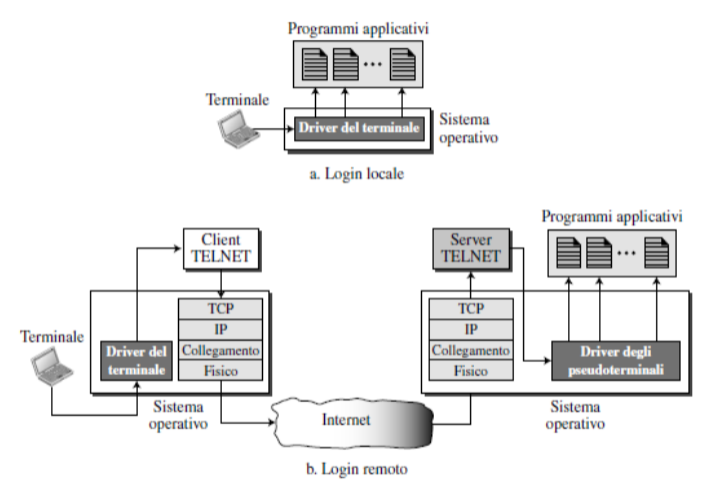
\includegraphics[scale=0.5]{assets/telnet.png}
	\end{center}

	\subsection{SSH - Secure Shell} 
	Il \textbf{Secure Shell} (SSH) è un protocollo di rete utilizzato per stabilire una connessione sicura tra un client e un server. Il protocollo SSH consente di accedere e controllare un computer remoto in modo sicuro, consentendo di eseguire comandi e interagire con il sistema remoto in modo crittografato. Il protocollo SSH è basato su una struttura client-server, in cui il client SSH invia comandi al server SSH per eseguire operazioni sul sistema remoto. Il protocollo SSH utilizza il protocollo TCP per garantire l'affidabilità e l'ordine dei dati, e utilizza la crittografia per proteggere i dati trasmessi tra il client e il server. Si divide in tre componenti:
	\begin{itemize}
		\item \textbf{SSH Transport-Layer Protocol}: crea e gestisce un canale di trasmissione sicuro sfruttando la connessione TCP.
		\item \textbf{SSH Authentication Protocol}: autentica il client e il server per garantire che entrambi siano legittimi.
		\item \textbf{SSH Connection Protocol}: gestisce le sessioni di shell interattive e non interattive tra il client e il server permettendo l'accesso al terminale, l'esecuzione remota e il trasferimento di file.
	\end{itemize}
	\begin{center}
		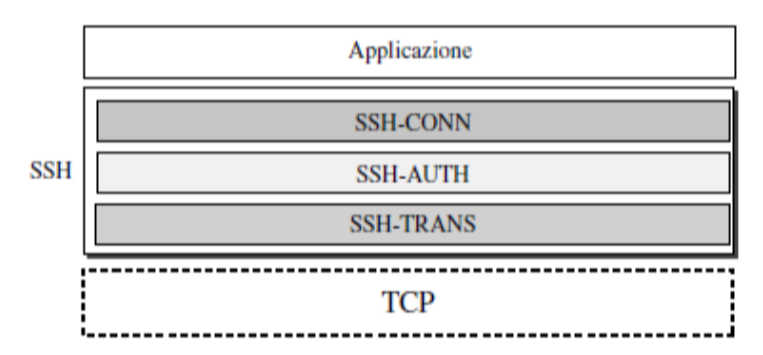
\includegraphics[scale=0.5]{assets/ssh.png}
	\end{center}

	\subsection{DNS - Domain Name System}
	I dispositivi connessi in rete vengono individuati dai protocolli dello stack TCP/IP mediante il loro indirizzo IP. Viene naturale pensare che ricordare un indirizzo IP sia più difficile che ricordare un nome, soprattutto quando si tratta di memorizzare un grande numero di indirizzi. Per ovviare a questo problema, è stato creato il \textbf{Domain Name System} (DNS), un sistema distribuito di risoluzione dei nomi che associa un nome di dominio a un indirizzo IP. Il DNS è un servizio di rete che consente di tradurre i nomi di dominio in indirizzi IP e viceversa.
	\begin{center}
		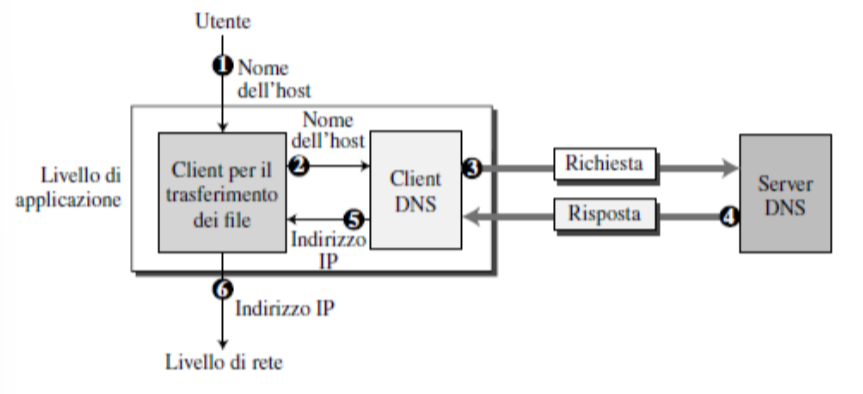
\includegraphics[scale=0.5]{assets/dns.png}
	\end{center}
	Il DNS è basato su una struttura gerarchica, in cui i nomi di dominio sono organizzati in un albero di dominio, con il dominio radice in cima all'albero. 
	\begin{center}
		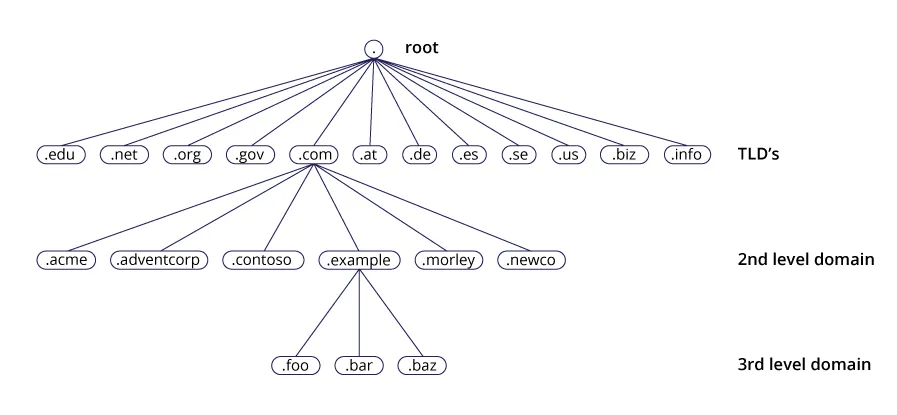
\includegraphics[scale=0.5]{assets/dns-tree.png}
	\end{center}
	I nomi di dominio sono composti da una serie di etichette separate da punti, con l'etichetta più a destra che rappresenta il dominio di primo livello (TLD), come .com, .org, .net, .it, ecc. 
	\begin{center}
		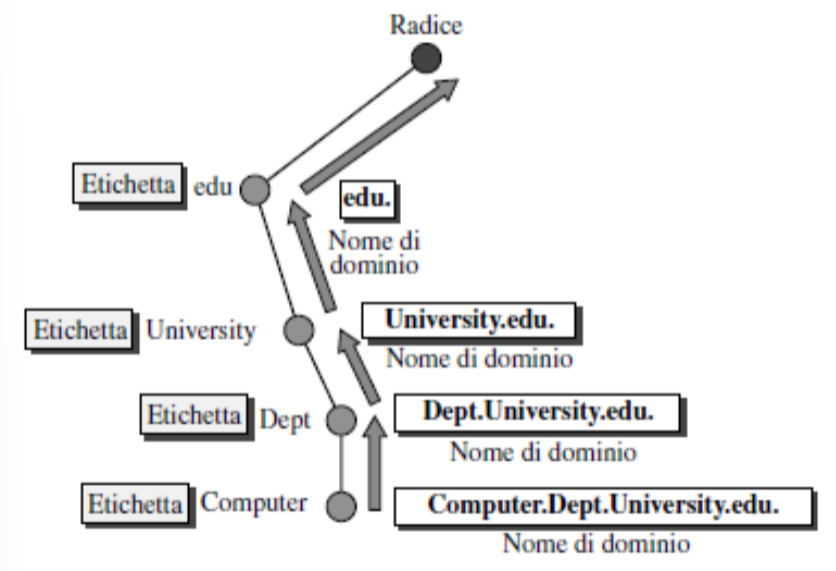
\includegraphics[scale=0.5]{assets/dns-label.png}
	\end{center}
	I nomi di dominio possono essere:
	\begin{itemize}
		\item \textbf{FQDN - Fully Qualified Domain Name}: un nome di dominio completo che specifica il dominio di primo livello, il dominio di secondo livello e tutti i sottodomini intermedi.
		\item \textbf{PQDN - Partially Qualified Domain Name}: un nome di dominio parziale che specifica solo il dominio di secondo livello e tutti i sottodomini intermedi.
	\end{itemize}
	\begin{center}
		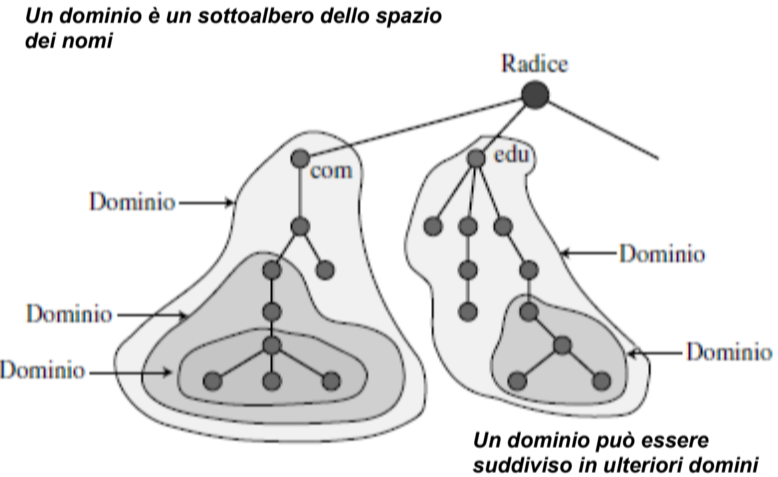
\includegraphics[scale=0.5]{assets/dns-fqdn.png}
	\end{center}

	\subsubsection{Address Resolution}
	Il DNS risolve i nomi di dominio in indirizzi IP utilizzando un processo chiamato \textbf{address resolution}. Quando un client richiede un nome di dominio, il client si rivolge al proprio DNS (resolver) per risolvere il nome di dominio in un indirizzo IP. Il resolver invia una richiesta al server DNS più vicino, il quale cerca il nome di dominio nel database DNS e restituisce l'indirizzo IP corrispondente al client. Se il server DNS non trova il nome di dominio nel proprio database, inoltra la richiesta ad un altro server DNS e così via fino a quando il nome di dominio viene risolto con successo. I Server DNS sono collegati fra di loro a livello mondiale e costituiscono una vera e propria rete di scambio e aggiornamento dati. Se quindi un amministratore di rete modifica il DNS, sarà necessario del tempo affinchè la modifica venga propagata a tutti i server DNS del mondo. Questo tempo è detto Tempo di Propagazione DNS e può variare da pochi minuti a 48 ore. Pur non essendo controllabile, è possibile tentare di ridurlo al minimo. La risoluzione può essere di due tipi:
	\begin{itemize}
		\item \textbf{ricorsiva}: il server DNS riceve una richiesta dal client e si occupa di trovare la risposta completa. Se il server non ha l'informazione necessaria, interroga altri server DNS fino a ottenere la risposta finale. Questo processo può coinvolgere più livelli di server, ma il client riceve direttamente la risposta dal server iniziale, senza preoccuparsi di altre richieste.
		\begin{center}
			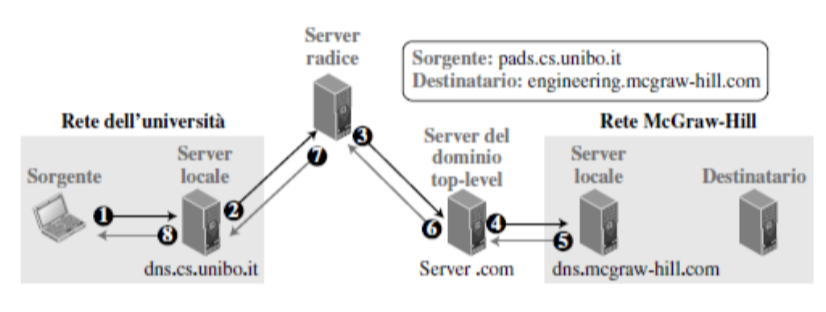
\includegraphics[scale=0.5]{assets/dns-rec.png}
		\end{center}
		\item \textbf{iterativa}:  il server DNS fornisce al client la migliore risposta possibile. Se non possiede l'informazione, restituisce l'indirizzo di un altro server DNS che potrebbe saperne di più. Il client quindi invia la richiesta a quel nuovo server. Questo processo continua finché non si trova la risposta, con il client che gestisce direttamente le varie richieste.
		\begin{center}
			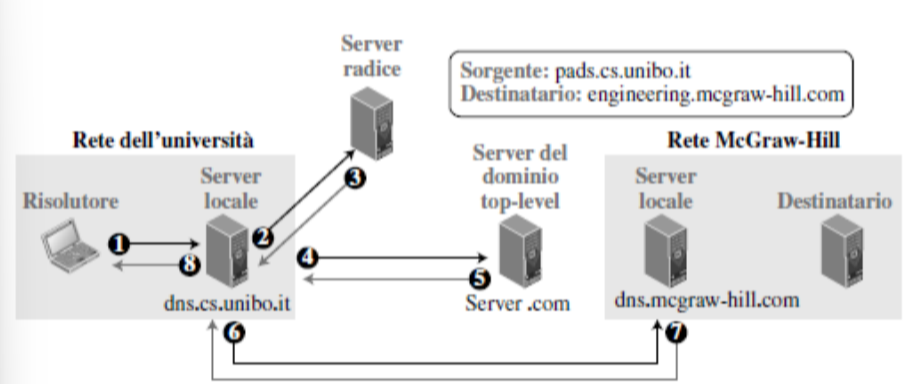
\includegraphics[scale=0.5]{assets/dns-iter.png}
		\end{center}
	\end{itemize}

	\subsubsection{Caching}
	Il DNS utilizza il \textbf{caching} per memorizzare le informazioni sui nomi di dominio risolti, riducendo il tempo di risoluzione e il traffico di rete. Quando un server DNS risolve un nome di dominio, memorizza l'associazione tra il nome di dominio e l'indirizzo IP in una cache locale. In questo modo, se un client richiede lo stesso nome di dominio in futuro, il server DNS può risolverlo rapidamente dalla cache locale senza dover interrogare altri server DNS. Il caching riduce il tempo di risoluzione e il traffico di rete, migliorando le prestazioni e l'efficienza del sistema DNS. Tuttavia, il caching può causare problemi se le informazioni memorizzate nella cache diventano obsolete o non corrispondono più alla configurazione attuale del DNS. Per evitare questo problema, i server DNS utilizzano il TTL per specificare la durata della memorizzazione nella cache.

	\subsubsection{TTL - Time To Live}
	Il \textbf{Time To Live} (TTL) è un valore numerico associato alla configurazione di un DNS che stabilisce il tempo dell'associazione tra un nome di dominio e un indirizzo IP al cui termine il server provvede ad aggiornarla. Il TTL è espresso in secondi e secondo le norme RFC2308 deve essere compreso tra 3600 e 86400 secondi. Un TTL basso comporterà che gli altri server DNS rispondano ad eventuali richieste non con i dati che hanno in cache, ma richiedendo un aggiornamento degli stessi. Ciò comporta un aumento del traffico e un rallentamento del servizio. Un TTL alto, invece, comporterà che i server DNS risponderanno con i dati in cache, riducendo il traffico e velocizzando il servizio. Tuttavia, un TTL alto comporta che eventuali modifiche ai record DNS non saranno visibili fino a che il TTL non sarà scaduto. TTL bassi vanno usati solo ed esclusivamente in caso di modifiche, altrimenti vanno usati TTL elevati.

	\subsubsection{Tipi di Record DNS}
	Il DNS utilizza diversi tipi di record per associare i nomi di dominio agli indirizzi IP e per fornire altre informazioni sui nomi di dominio. Alcuni dei record DNS più comuni sono:
	\begin{itemize}
		\item \textbf{A}: associa un nome di dominio a un indirizzo IPV4.
		\item \textbf{NS}: specifica i server DNS autoritativi per un dominio.
		\item \textbf{CNAME}: specifica un nome di dominio alias (alternativo) per un nome di dominio ufficiale (canonico).
		\item \textbf{SOA}: specifica le informazioni autoritative per un dominio.
		\item \textbf{MX}: specifica i server di posta elettronica per un dominio.
		\item \textbf{AAAA}: associa un nome di dominio a un indirizzo IPV6.
	\end{itemize}

	\subsubsection{Struttura messaggi DNS}
	\begin{center}
		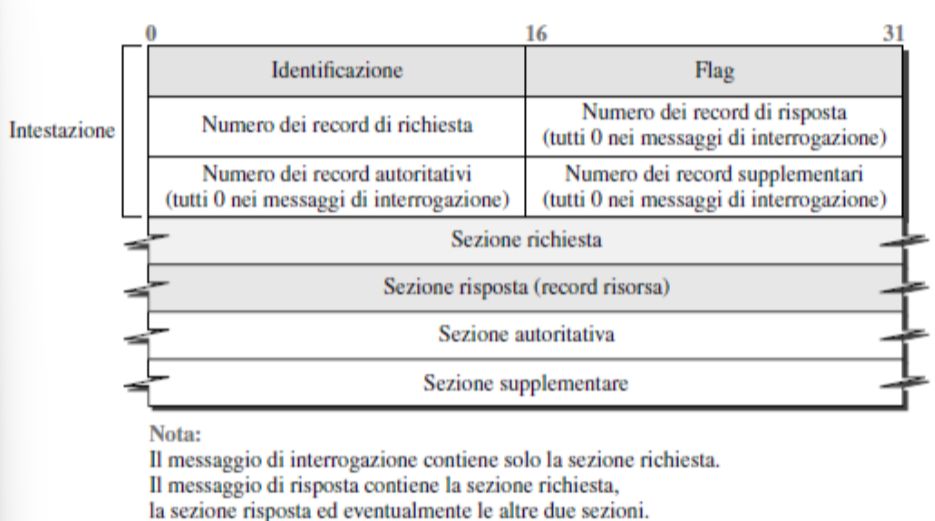
\includegraphics[scale=0.5]{assets/dns-msg.png}
	\end{center}

	\chapter{Livello Trasporto}
	Il livello di trasporto nello stack TCP/IP è situato fra il livello applicazione e il livello rete ed è responsabile della comunicazione end-to-end tra i processi applicativi tramite un collegamento logico. Il livello di trasporto fornisce servizi di trasporto affidabili e non affidabili per il trasferimento dei dati tra i processi applicativi e riceve servizi dal livello di rete. 
	
	\section{Servizi del livello trasporto}
	Il primo compito del livello di trasporto è supportare la comunicazione tra processi. Un processo è un'entità in esecuzione di livello applicazione che usa i servizi del livello di trasporto per comunicare con altri processi.
	\begin{center}
		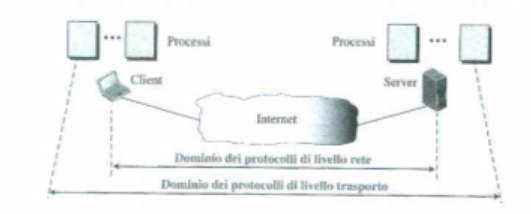
\includegraphics[scale=0.5]{assets/trans-comm.png}
	\end{center}
	Il livello rete si occupa della comunicazione tra dispositivi (host) consegnando i messaggi al destinatario. Ma questa consegna è incompleta perchè i messaggi devono giungere ai processi cui erano indirizzati (sullo stesso host possono essere attivi svariati processi applicativi). E' a qusto punto che intervengono i protocolli del livello di trasporto.

	\subsection{Indirizzamento: Porte}
	Sebbene la comunicazione tra processi possa essere realizzata in diversi modi, la più diffusa è quella basara sul paradigma client/server. Un processo sul client necessita di servizi svolti da un processo su un server. I due processi, client e server, hanno lo stesso nome e si identificano tramite un indirizzo IP. Tuttavia, poichè su un host possono essere attivi più processi, è necessario un ulteriore identificativo, la \textbf{porta}. 
	\vspace{\baselineskip}\\
	Una porta è un numero a 16 bit, nell'intervallo 0 - 65535, che identifica un processo su un host. Al client viene assegnata una porta casuale, detta \textbf{porta effimera}, mentre al server viene assegnata una porta nota. Le porte note sono quelle che identificano i servizi più comuni, come la porta 80 per HTTP, la porta 21 per FTP, la porta 25 per SMTP, ecc. Le porte effimere sono quelle che identificano i processi client. Le porte sono divise in tre categorie:
	\begin{itemize}
		\item \textbf{Porte note}: 0 - 1023, riservate ai protocolli standard e sono assegnate dall'authority ICANN.
		\item \textbf{Porte registrate}: 1024 - 49151, non gestite da ICANN e servono per evitare duplicati tra servizi specifici.
		\item \textbf{Porte dinamiche}: 49152 - 65535, assegnate dinamicamente dal sistema operativo e possono essere usati come numeri di porta temporanei o privati.
	\end{itemize}
	\begin{center}
		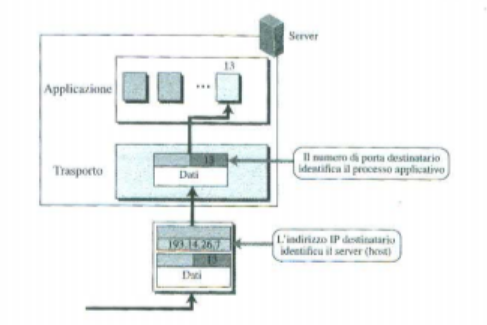
\includegraphics[scale=0.5]{assets/port.png}
	\end{center}

	\subsection{Socket Address}
	Un protocollo del livello trasporto nello stack TCP/IP necessita di due identifictori per ogni lato, l'indirizzo IP e il numero di porta. La loro combinazione è detta \textbf{socket address} che identifica univocamente il processo client, se si tratta di socket address client, o server, se si parla di socket address server. L'indirizzo IP identifica l'host, mentre il numero di porta identifica il processo. Affinchè si possano utilizzare i servizi del livello trasporto è necessaria una coppia do socket address: quello del client e quello del server. queste 4 informazioni sono contenute negli header dei pacchetti del livello rete e livello trasporto, più precisamente il primo header contiene gli indirizzi Ip, mentre il secondo contiene le porte.

	\subsection{Incapsulamento/Decapsulamento}
	Per inviare un messaggio da un processo ad un altro, il protocollo di livello trasporto incapsula e decapsula i messaggi. L'incapsulamento avviene lato mittente, partendo dal processo applicativo, passando per il livello di trasporto, il livello di rete e il livello fisico. Il decapsulamento avviene lato destinatario, partendo dal livello fisico, passando per il livello di rete, il livello di trasporto e infine il processo applicativo. Quando un processo deve inviare un messaggio, lo passa al livello trasporto insieme a una coppia di socket address e ad altre informazioni, ch edipendono dal potocollo del livello trasporto. Il livello trasporto riceve i dati e vi aggiunge il proprio header incapsulando il tutto in un pacchetto del livello trasporto. I pacchetti a livello trasporto sono chiamati \textbf{segmenti (in TCP)} o \textbf{datagrammi utente (in UDP)}. Il decapsulamento è il processo inverso nel quale si andrà a rimuovere l'header del livello trasporto e si passerà i dati al processo applicativo.

	\subsection{Multiplexing e Demultiplexing}
	Il livello di trasporto deve essere in grado di gestire la comunicazione tra più processi su un host. Per fare ciò, il livello di trasporto utilizza il \textbf{multiplexing} e il \textbf{demultiplexing}. Il multiplexing fa riferimento al caso in cui un'entità riceve informazioni da più di una sorgente; il demultiplexing fa riferimento al caso in cui un'entità invia informazioni a più di una destinazione. Il multiplexing e il demultiplexing sono responsabili di associare i dati in arrivo al processo corretto e di inviare i dati in uscita al destinatario corretto. Il multiplexing e il demultiplexing sono gestiti dalle porte. Quando un pacchetto arriva a un host, il livello di trasporto utilizza il numero di porta di destinazione per instradare il pacchetto al processo corretto. Quando un processo invia un pacchetto, il livello di trasporto utilizza il numero di porta di origine per identificare il processo mittente. Il multiplexing e il demultiplexing consentono al livello di trasporto di gestire la comunicazione tra più processi su un host.
	\begin{center}
		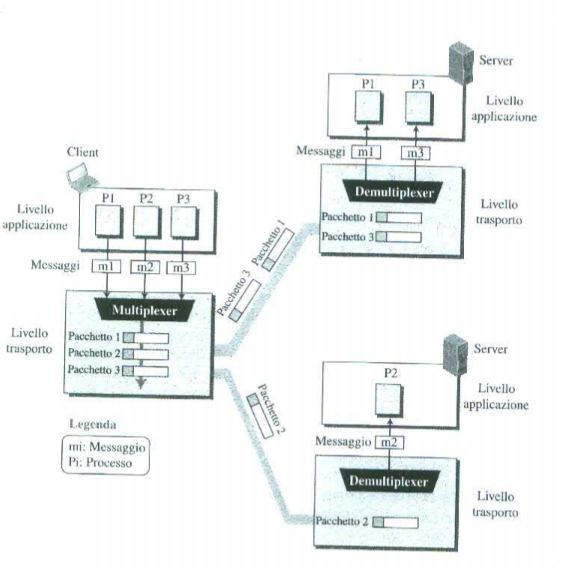
\includegraphics[scale=0.5]{assets/multipl-demultipl.png}
	\end{center}

	\subsection{Controlli di flusso}
	Quando un'entità produce dati che un'altra entità deve consumare, deve esistere un equilibrio fra la velocità di produzione e la velocità di consumo dei dati. Se i dati vengono prodotti a una velocità superiore rispetto a quella con cui possono essere consumati, il consumatore potrebbe trovarsi sovraccaricato ed essere costretto ad eliminarne alcuni. Se i dati vengono prodotti ad una velocità inferiore rispetto a quella con cui possono essere consumati, il consumatore deve rimanere in attesa, riducendo l'efficienza del sistema. Il \textbf{controllo di flusso} è un meccanismo che regola la velocità di trasmissione dei dati tra mittente e destinatario in modo da garantire che il mittente non invii dati più velocemente di quanto il destinatario possa riceverli. 
	\subsection*{Produttore/Consumatore}
	Nella comunicazione al livello trasporto si ha a che fare con quattro entità:
	\begin{itemize}
		\item processo mittente
		\item livello trasporto mittente
		\item livello trasporto destinatario
		\item processo destinatario
	\end{itemize}
	Il processo mittente a livello applicazione è solo un produttore di dati che vengono passati al livello trasporto mittente. Quest'ultimo è sia un produttore che un consumatore di dati, in quanto riceve i dati dal processo mittente, li incapsula e li passa al livello trasporto destinatario. Quest'ultimo è sia un produttore che un consumatore di dati, in quanto riceve i dati dal livello trasporto mittente, li decapsula e li passa al processo destinatario. Il processo destinatario è solo un consumatore di dati che riceve i dati dal livello trasporto destinatario.
	\begin{center}
		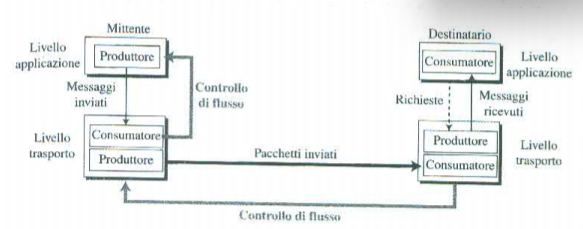
\includegraphics[scale=0.5]{assets/prod-cons.png}
	\end{center}
	Nella comunicazione sono necessari almeno due casi di controllo di flusso: uno tra il livello trasporto mittente e il processo mittente e uno tra il livello trasporto destinatario e il livello trasporto mittente.  Sebbene il controllo el flusso possa essere realizzato in modi differenti, una delle soluzioni più comuni consiste nell'utilizzare due \textbf{buffer}, uno a livello trasporto mittente e uno a livello trasporto destinatario. Un buffer è una zona di memoria temporanea utilizzata per memorizzare i dati in arrivo o in partenza. La comunicazione delle informazioni di controllo del flusso può avvenire inviando segnali dal consumatore al produttore. Il livello di trasporto del mittente segnala al livello applicazione, quando ha il buffer saturo, di sospendere l'invio di messaggi; quando si libera dello spazio nel buffer segnala al livello applicazione di riprendere l'invio di messaggi. Il livello di trasporto del destinatario segnala al livello trasporto del mittente, quando il buffer è pieno, di sospendere l'invio di pacchetti; quando si libera dello spazio nel buffer segnala al livello trasporto del mittente di riprendere l'invio di pacchetti.

	\subsection{Controllo degli errori}
	In Internet, considerato che il livello rete è inaffidabile, è necessario implementare l'affidabilità al livello trasporto se richiesta dall'applicazione. L'affidabilità può essere ottenuta aggiungendo i servizi di controllo degli errori al livello trasporto, i quali hanno il compito di rilevare e scartare pacchetti corrotti, tenere traccia dei pacchetti persi e scartati e gestirne la rispedizione, riconoscere i pacchetti duplicati ed eliminarli, bufferizzare i pacchetti fuori sequenza fino a quando arrivano i pacchetti mancanti.\\
	Il controllo degli errori, a differenza del controllo di flusso, coinvolge solamente i livelli trasporto del mittente e del destinatario. Si suppone, infatti, che i messaggi scambiati fra i livelli applicazione siano esenti da errori. \\
	Il controllo degoi errori comporta che il livello trasporto del mittente sappia quale pacchetto debba rispedire e che il livello trasporto del destinatario sappia riconoscere i pacchetti duplicati o fuori sequenza. Questo può essere ottenuto numerando i pacchetti tramite il campo \textbf{sequence number (numero di sequenza)}. Quando un pacchetto viene corrotto o smarrito, identificandolo tramite il numero di sequenza, il livello trasporto del destinatario può chiedere al livello trasporto del mittente di rispedirlo. Il livello trasporto del destinatario può identificare anche i pacchetti duplicati (con il medesimo numero di sequenza) e decidere di scartarne uno. I pacchetti fuori sequenza possono essere identificati verificando gli eventuali numeri di sequenza ricevuti disordinatamente.\\
	I pacchetti vengono numerati sequenzialmente. Tuttavia, poichè è necessario inserire il numero di sequenza in ogni header di pacchetto, occorre specificarne il valore massimo. Se l'header prevede massimo $m$ bit per il numero di sequenza, il valore massimo sarà $2^m - 1$. Se il numero di sequenza raggiunge il valore massimo, deve essere riportato a 0. Questo comporta che i numeri di sequenza sono considerati in modulo.\\
	Per notificare al mittente la corretteza della ricezione di uno o pià pacchetti viene utilizzato il \textbf{numero di riscontro (acknowledgement number - ACK)}. Il destinatario può semplicemente scartare i pacchetti corrotti. Il mittente può identificare i pacchetti persi utilizzando un timer: quando invia un pacchetto, il mittente avvia un timer, se non riceve l'ACK entro il tempo limite, il mittente rispedisce il pacchetto.

	\subsection{Integrazione del controllo degli errori e del controllo di flusso}
	Per combinare il controllo degli errori e il controllo di flusso, vengono utilizzati due buffer numerati, uno presso il mittente e uno presso il destinatario. Nel mittente, quando si prepara un pacchetto si usa il numero della posizione libera successiva nel buffer, x, come numero di sequenza del pacchetto. Quando il pacchetto viene inviato, ne viene memorizzata una copia nella locazione x, in attesa della sua conferma da parte del destinatario. Quando si riceve una conferma relativa al pacchetto inviato, il pacchetto memorizzato nel buffer viene eliminato liberando la posizione di memoria che occupava. Nel destinatario, quando si riceve un pacchetto con numero di sequenza y, si controlla se y è il numero di sequenza atteso. Se lo è, il pacchetto viene consegnato al processo destinatario e si invia un ACK con numero di riscontro uguale a y. 
	\vspace{\baselineskip}\\
	Il buffer viene rappresentato come un insieme di settori, chiamati \textbf{finestra scorrevole (sliding window)}, che in ogni istante occupano una parte del buffer. Nel mittente, quando viene inviato un pacchetto se ne contrassegna il settore corrispondente. Quando tutti i settori sono contrassegnati, il buffer è completo e non possono essere accettati altri messaggi dal livello applicazione. Quando arriva un riscontro, viene eliminato il contrassegno dal settore corrispondente. Quando un insieme consecutivo di settori a partire dall'inizio della finestra non risulta contrassegnato, la finestra scorre sopra l'intervallo dei numeri di sequenza corrispondenti rendendo disponibile un numero di settori equivalente alla fine della dinestra.
	\vspace{\baselineskip}\\
	La finestra scorrevole è solo un'astrazione: in realtà si utilizzano delle variabili per contenere i numeri di sequenza del pacchetto successivo da inviare e dell'ultimo pacchetto inviato.

	\subsection{Controllo della congestione}
	Una questione importante nelle reti a commutazione di paccheto come Internet, è la \textbf{congestione}. Essa può avvenire se il carico della rete, cioè il numero di pacchetti inviati alla rete, è superiore alla capacità della rete, cioè il numero di pacchetti che una rete può gestire. Il controllo della congestione attua meccanismi e tecniche per controllare la congestione mantenendo il carico della rete al di sotto della sua capacità. La congestione può avvenire in qualsiasi sistema che comporti attesa, poichè router e switch hanno buffer dove vengono memorizzati i pacchetti prima e dopo la loro elaborazione. Un router, per esempio, ha una coda di input ed una di output per ogni interfaccia. Se esso non riesce ad elaborare i pacchetti alla stessa velocità con la quale i pacchetti arrivano, la coda di input si sovraccarica e si crea la congestione.

	\subsection{Servizi Connection Oriented e Connectionless}
	Un protocollo del livello di trasporto può fornire due tipi principali di servizi, noti come \textbf{connection-oriented} e \textbf{connectionless}. Questi servizi rispondono a esigenze diverse di comunicazione e trasmissione dei dati tra dispositivi collegati in rete, offrendo opzioni sia per connessioni affidabili e strutturate, sia per invii di dati più flessibili e senza connessione stabile. La scelta tra i due tipi di servizio dipende da vari fattori, tra cui le specifiche dell'applicazione, i requisiti di rete e la priorità tra affidabilità e rapidità nella trasmissione dei dati.

	\subsubsection{Connectionless}
	In un \textbf{servizio connectionless} il processo mittente deve dividere i suoi messaggi in porzioni di dimensioni accettavili dal livello trasporto, a cui consegnarli uno a uno. Il livello trasporto tratta ogni porzione coome entità singola senza mantenere alcuna relazione fra di esse. Quando una porzione arriva dal livello applicazione, il livello trasprto la incapsula in un pacchetto e la invia.
	\vspace{\baselineskip}\\
	Si supponga che un processo client abbia un messaggio diviso in tre parti da inviare ad un processo server. Le varie porzioni sono consegnate al protocollo di trasporto privo di connessione in ordine. Tuttavia, poichè non vi è alcuna relaizone fra i diversi pacchetti a livello trasporto, i pacchetti potrebbero arrivare a destinazione fuori sequenza ed essere quindi ocnsegnati al processo server nell'ordine errato. La situazione sarebbe peggiore se uno dei pacchetti venise perso. Poichè i pacchetti non sono numerati, il livello trasporto destinatario non avrebbe modo di sapere che uno dei pacchetti è mancante.
	\vspace{\baselineskip}\\
	I due problemi nascono dal fatto che i due livelli di trasporto non  si coordinano l'uno con l'altro. Di conseguenza risulta impossibile implementare efficacemente il controllo di flusso, di errori o di congestione in un sistema connectionless
	\begin{center}
		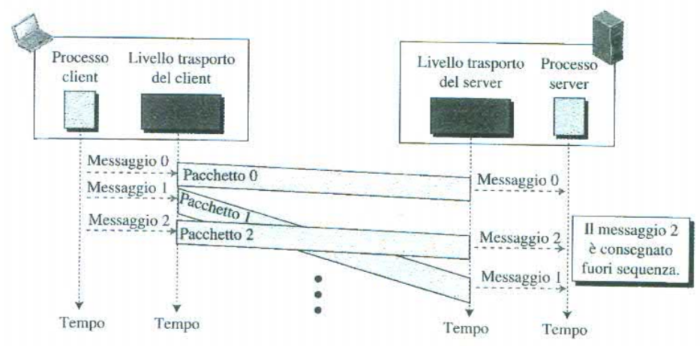
\includegraphics[scale=0.5]{assets/connless.png}
	\end{center}

	\subsubsection{Connection Oriented}
	In un \textbf{servizio connection-oriented}, il client e il server devono per prima cosa stabilire una connessione \textbf{logica}. Solo dopo questa fase i due processi possono scambiarsi i dati. Una volta terminato lo scambio di dati, la connessione logica viene chiusa. Grazie alla connessione logica, il livello trasporto può garantire che i pacchetti vengano consegnati al destinatario nell'ordine corretto e senza duplicati. Inoltre, se un pacchetto viene perso, il mittente può rispedirlo. La connessione logica permette anche di implementare il controllo di flusso, di errori e di congestione.
	\begin{center}
		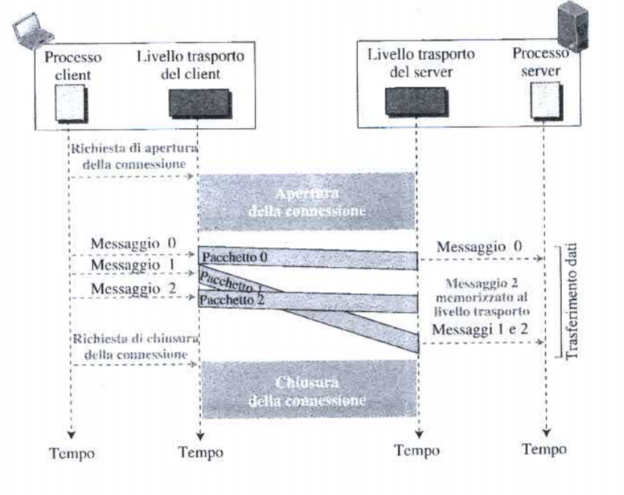
\includegraphics[scale=0.5]{assets/conn-orie.png}
	\end{center}

	\section{Protocolli di livello trasporto}
	E' possibile sviluppare un protocollo di livello trasporto combinando un inseime di servizi descritti in precedenza. Lo stack TCP/IP usa protocolli di livello trasporto che sono una combinazione o una variante di alcuni meccanismi che stiamo per analizzare.

	\subsection{Protocollo semplice}
	Un protocollo di livello trasporto semplice può essere realizzato privo di connessione, senza controllo degli errori e del flusso. Quindi, si presuppone che il destinatario sia in grado di gestire immediatamente tutti i pacchetti ricevuti. In altre parole, il destinatario non viene mai sovraccaricato da pacchetti in arrivo. Il livello trasporto mittente riceve un pacchetto dal proprio processo applicativo, lo incapsula in un pacchetto di livello trasporto e lo invia al destinatario. Il livello trasporto destinatario riceve il pacchetto, lo decapsula e lo passa al processo applicativo. Si gestisce quindi solo la trasmissione dei pacchetti, senza preoccuparsi di errori, flusso o congestione. Il mittente non può inviare pacchetti ifno a quando il suo livello applicazione non ha un messaggio da spedire, analogamente il destinatario non può consegnare un messaggio al proprio livello applicazione se non ha ricevuto un pacchetto. Il protocollo UDP corrisponde ad una lieve variante di questo protocollo.
	\begin{center}
		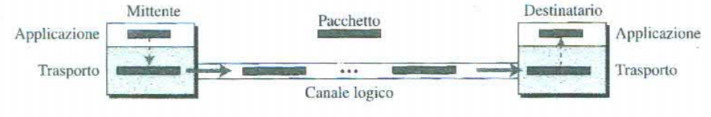
\includegraphics[scale=0.5]{assets/simple-prot.png}
	\end{center}

	\subsection{Stop and Wait}
	Il secondo meccanismo preso in considerazione è orientato alla connessione ed è chiamato \textbf{stop-and-wait}. In questo meccanismo sono implementati il ocntrollo di flusso e degli errori e mittente e destinatario usano entrambi una finestra scorrevole di dimensione 1. Il mittente invia un pacchetto alla volta e aspetta un ACK dal destinatario prima di inviarne un altro. Per rilevare pacchetti corrotti è necessario aggiungere un valore di \textit{checksum} a ogni pacchetto dati. Quando un pacchetto arriva al destinatario viene calcolato il checksum: se il valore corrisponde al checksum ricevuto, il destinatario invia un ACK al mittente, altirmenti il pacchetto viene scartato senza informare il mittente. Se il mittente non riceve l'ACK entro un tempo limite (timer), rispedisce il pacchetto. Il timer viene azzerato ogni volta che il mittente riceve un ACK. Questo comporta che il mittente deve memorizzare una copia del pacchetto inviato finchè non riceve l'ACK.
	\begin{center}
		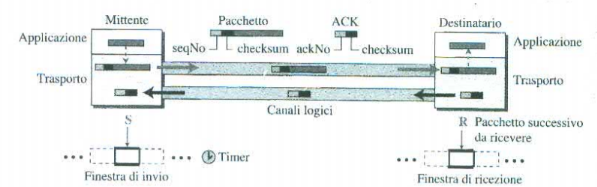
\includegraphics[scale=0.5]{assets/stop-wait.png}
	\end{center}
	Per poter gestire i pacchetti duplicati, lo Stop and Wait utilizza i numeri di sequenza e di riscontro. Viene quindi aggiunto un campo all'header del pacchetto per contenere il valore del numero di sequenza del pacchetto. Poichè i numeri di sequenza devono essere adatti sia per numerare i pacchetti sia per indicare i riscontri, si utilizza la seguente convenzione: il numero di riscontro indica sempre il numero di sequenza del prossimo pacchetto atteso dal destinatario. Per ottimizzare la dimensione dei campi nell'header si possono utilizzare 0 e 1 come valori per i numeri di sequenza e di riscontro. Se il destinatario ha ricevuto correttamente il pacchetto con numero di sequenza 0, invierà un ACK con numero di riscontro 1. Se invece ha ricevuto correttamente il pacchetto con numero di sequenza 1, invierà un ACK con numero di riscontro 0.
	\vspace{\baselineskip}\\
	Il meccanismo Stop and Wait è molto inefficiente se il canale ha velocità di trasmissione elevata e lungo ritardo.

	\subsection{Go-Back-N (GBN)}
	Nello Stop and Wait il mittente deve attendere che il pacchetto precedente abbia raggiunto il destinatario e che il relativo riscontro sia stato ricevuto prima di poter inviare il pacchetto successivo. Tuttavia, per aumentare l'efficienza di trasmissione si devono avere più pacchetti in transizione mentre il mittente è in attesa dei riscontri. In altre parole, è necessario consentire di lasciare in sospeso (in attesa di riscontro) più di un pacchetto, mantenendo il canale occupato mentre il mittente è in attesa dei riscontri. 
	\vspace{\baselineskip}\\
	Questo è realizzato dal meccanismo \textbf{Go-Back-N}. Questo meccanismo, così come il \textit{Selective Repeat} (che vedremo in seguito), adotta la tecnica del \textbf{pipeling} permettendo di inviare più pacchetti senza dover attenderre il riscontro ai primi pacchetti inviati. D'altronde il destinatario può bufferizzare un solo pacchetto alla volta, quindi il mittente deve essere in grado di memorizzare una copia di tutti i pacchetti inviati in attesa di riscontro, fino a quando non riceve il riscontro.
	\vspace{\baselineskip}\\
	In GBN i numeri di sequenza sono calcolati in modulo $2^m$, dove $m$ è la dimensione del campo sequence number in bit. Il numero di riscontro in questo meccanismo è cumulativo e indica il numero di sequenza del prossimo pacchetto atteso. Per esempio, se il numero di riscontro vale 7, significa che tutti i pacchetti fino al 6 sono stati ricevuti correttamente e che il destinatario si attende di ricevere il pacchetto con numero di sequenza 7.
	\vspace{\baselineskip}\\
	La \textbf{finestra di invio} contiene i numeri di sequenza dei pacchetti che possono essere in transito o spediti. Per ciascuna posizione di questa finestra, alcuni dei numeri di sequenza corrispondono ai pacchetti inviati, altri corrispondono a quelli che possono essere inviati. La diimensione massima della finestra di invio è $2^m - 1$. La finestra di invio in ogni istante divide i possibili numeri di sequenza in quattro regioni: la prima è la regione dei numeri di sequenza che corrispondono ai pacchetti inviati, confermati ed eliminati dal buffer; la seconda definisce l'intervallo dei numeri di sequenza dei pacchetti che sono stati inviati ma con stato ancora ignoto, quindi in attesa di riscontro; la terza definisce l'intervallo dei numeri di sequenza dei pacchetti che possono essere inviati ma privi di dati corrispondenti al livello applicazione; la quarta definisce l'intervallo dei numeri di sequenza dei pacchetti che non possono essere utilizzati fino a quando la finestra non avanza.	
	\begin{center}
		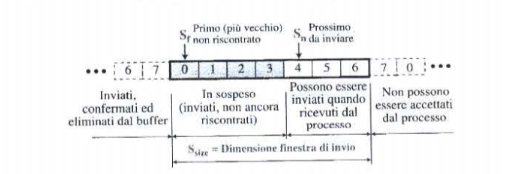
\includegraphics[scale=0.7]{assets/gbn.png}
	\end{center}
	La finestra è un concetto astratto: tre variabili ne definiscono le dimensioni e la posizione in ogni istante: $S_f$ (send first) ovvero il primo pacchetto in attesa di riscontro nella finestra di invio, $S_n$ (send next) ovvero il numero di sequenza da assegnare al prossimo pacchetto da inviare e $S_{size}$ (send size) ovvero la dimensione della finestra di invio.
	\vspace{\baselineskip}\\
	La \textbf{finestra di ricezione} permette di ricevere i pacchetti dati corretti e inviare i relativi riscontri. Nel GBN la dimensione della finestra di ricezione è sempre 1. Il destinatario è sempre in attessa dell'arrivo di un pacchetto specifico. Qualsiasi pacchetto arrivato fuori sequenza viene scartato e deve essere rispedito. La finestra di ricezione è definita da una sola variabile $R_n$ (receive next) che indica il numero di sequenza del prossimo pacchetto atteso. I numeri di sequenza a sinistra della finestra indicano i pacchetti già ricevuti e riscontrati; i numeri di sequenza a destra della finestra indicano i pacchetti che non possono essere ancora ricevuti. Qualsiasi pacchetto con numero di sequenza a sinistra o a destra della finestra viene scartato.Viene accettato solamente il pacchetto con numero di sequenza uguale a $R_n$.
	\begin{center}
		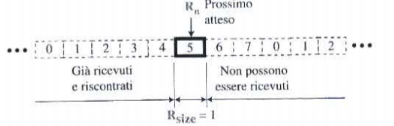
\includegraphics[scale=0.7]{assets/gbn2.png}		
	\end{center}
	Sebbene vi possa essere un timer per ciascun pacchetto inviato, nel GBN se ne usa solo uno poichè il timer del primo pacchetto in attesa di riscontro scade sempre per primo. Quando esso scade, si rispediscono tutti i pacchetti in attesa di riscontro. Questo è il motivo per cui si chiama Go-Back-N: se un pacchetto viene perso, il mittente rispedisce tutti i pacchetti a partire da quello perso.

	\subsection{Selective Repeat (SR)}
	Il GBN semplifica i compiti del destinatario, che tiene traccia di una sola variabile e non deve bufferizzare i pacchetti fuori frequenza. Questo meccanismo è tuttavia inefficiente se il livello rete sottostante perde numerosi pacchetti. Ogni volta che un singolo pacchetto risulta corrotto o smarrito, il mittente deve inviare tutti i pacchetti in attesa di riscontro anche se alcuni di questi sono già stati ricevuti correttamente ma fuori sequenza. Se il livello di rete perde numerosi apcchetti a causa della congestione, la rispediione di tutti i pacchetti in attesa peggiorerebbe la situazione comportando la perdita di un numero maggiore di pacchetti. Per ovviare a questo problema si utilizza il meccanismo \textbf{Selective Repeat}. Nel SR, vengono rispediti i pacchetti selettivamente, ovvero solo quelli realmente smarriti.
	\vspace{\baselineskip}\\
	Nel SR, il mittente mantiene una finestra di invio e il destinatario mantiene una finestra di ricezione. La dimensione della finestra di invio e di ricezione è $2^{m-1}$, dove $m$ è la dimensione del campo sequence number in bit. La finestra di ricezione del SR è totalmente differente da quella del GBN. la dimensione della finestra di ricezione è la stessa della finestra di invio e il SR permette a un numero di pacchetti uguale alla dimensione della finestra di arrivare fuori sequenza; i pacchetti vengono memorizzati nella finestra fino a quando si forma un blocco di pacchetti consecutivi da passare al livello applicazione. Poichè la dimensione delle finestre di invio e ricezoione è la stessa, tutti i pacchetti nella finestra di invio possono arrivare fuori sequenza ed essere memorizzati fino a quando possono essere consegnati.
	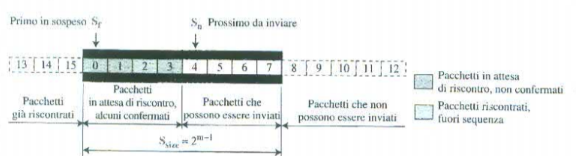
\includegraphics[scale=0.6]{assets/sr.png}
	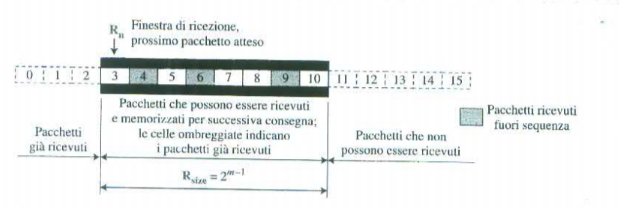
\includegraphics[scale=0.5]{assets/sr2.png}
	Teoricamente il SR usa un timer per ciascun pacchetto in attesa di riscontro: quanto un timer scade ne viene rispedito solo il relativo pacchetto. A differenza di GBN che gestisce i pacchetti in attesa di riscontro come un singolo gruppo, SR li gestisce individualmente. La maggior parte dei protocolli di trasporto che implementano SR usa tuttavia un solo timer.
	\vspace{\baselineskip}\\
	Nel SR il numero di riscontro indica il numero di un singolo pacchetto ricevuto correttamente, non può fornire feedback per gli altri.

	\subsection{Piggybacking}
	I quattro meccanismi finora discussi sono tutti unidirezionali: i pacchetti scorrono solo in una direzione e i riscontri nella direzione opposta. I pacchetti dati vengono in realtà trasmessi solitamente in entrambe le direzioni: dal client al server e viceversa. Questo significa che anche i riscontri devnon viaggiare in entrambe le direzioni.
	\vspace{\baselineskip}\\
	Per migliorare l'efficienza dei protocolli bidirezionali viene utilizzata una teecnica chiamata \textbf{piggybacking}. Il piggybacking consiste nel trasmettere un pacchetto di riscontro insieme a un pacchetto dati. Se il mittente ha un pacchetto dati da inviare e un pacchetto di riscontro da inviare, può trasmetterli insieme. Il destinatario riceve il pacchetto dati, lo decapsula e lo passa al livello applicazione. Il destinatario riceve anche il pacchetto di riscontro, lo decapsula e lo passa al livello trasporto.
	\begin{center}
		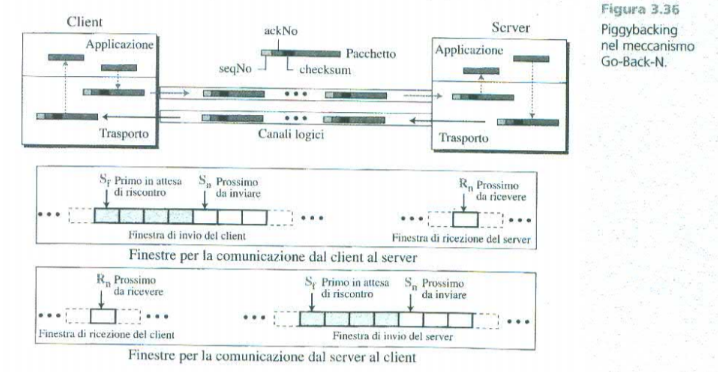
\includegraphics[scale=0.5]{assets/piggybacking.png}
	\end{center}

	\subsection{Protocolli Internet di livello trasporto}
	Dopo aver discusso degli aspetti teorici dei protocolli di livello trasporto, vediamo ora come questi aspetti sono implementati nei protocolli di livello trasporto usati in Internet. I due protocolli di livello trasporto più comunemente usati in Internet sono \textbf{TCP} e \textbf{UDP}. Questi due protocolli sono situati fra il livello applicazione e il livello rete e agiscono da intermediari fra i programmi applicativi e le operazioni della rete.
	\vspace{\baselineskip}\\
	UDP è un protocollo di trasporto connectionless e inaffidabile, utilizzato per la sua semplicità ed efficienza nei casi in cui il controllo degli errori può essere gestito dai processi di livello applicazione.
	\vspace{\baselineskip}\\
	TCP è un protocollo di trasporto connection-oriented e affidabile, che può essere utilizzato nelle applicazioni dove l'affidabilità è particolarmente importante.
	\vspace{\baselineskip}\\
	In entrambi i casi, uno dei principali compiti è quello di offrire un servizio di comunicazione tra processi: a tal fine questi protocolli utilizzano i numeri di porta:
	\begin{table}[H]
		\begin{tabular}{|c|c|c|c|p{9cm}|}
		\hline
		\textbf{Porta} & \textbf{Protocollo} & \textbf{UDP} & \textbf{TCP} & \textbf{Descrizione} \\
		\hline
		7   & Echo       & \checkmark & \checkmark & Rispedisce al mittente il datagramma ricevuto. \\
		9   & Discard    & \checkmark & \checkmark & Scarta tutti i datagrammi che vengono ricevuti. \\
		11  & Users      &            & \checkmark & Utenti attivi. \\
		13  & Daytime    & \checkmark & \checkmark & Restituisce l'ora e la data. \\
		17  & Quote      & \checkmark & \checkmark & Restituisce il messaggio del giorno (usato per debug). \\
		19  & Chargen    & \checkmark & \checkmark & Restituisce una stringa di caratteri. \\
		20, 21 & FTP     &            & \checkmark & File Transfer Protocol. \\
		23  & TELNET     &            & \checkmark & Terminal Network. \\
		25  & SMTP       &            & \checkmark & Simple Mail Transfer Protocol. \\
		53  & DNS        & \checkmark & \checkmark & Domain Name Service. \\
		67  & DHCP       & \checkmark &            & Dynamic Host Configuration Protocol. \\
		69  & TFTP       & \checkmark &            & Trivial File Transfer Protocol. \\
		80  & HTTP       &            & \checkmark & Hypertext Transfer Protocol. \\
		111 & RPC        & \checkmark & \checkmark & Remote Procedure Call (chiamata di procedura remota). \\
		123 & NTP        & \checkmark &            & Network Time Protocol. \\
		161, 162 & SNMP  & \checkmark &            & Simple Network Management Protocol. \\
		\hline
		\end{tabular}
	\end{table}

	\subsection{User Datagram Protocol (UDP)}
	\textbf{UDP} è un protocollo di livello trasporto connectionless e inaffidabile. Non aggiunge nulla ai servizi di IP eccetto la comunicazione tra processi. A discapito di questo, UDP è un protocollo molto semplice con un overhead minimo. Se un processo vuole inviare un piccolo messaggio senza preoccuparsi dell'affidabilità, può utilizzare UDP poichè l'invio richiede meno iterazioni fra mittente e destinatario rispetto a TCP.

	\subsubsection{Datagramma Utente UDP}
	I pacchetti UDP sono chiamati \textbf{datagrammi utente}. Ogni datagramma utente contiene l'header che è composto da un campo di 16 bit per la porta di origine, un campo di 16 bit per la porta di destinazione, un campo di 16 bit per la lunghezza del datagramma e un campo di 16 bit per il checksum. Il campo di lunghezza del datagramma include l'header e i dati. Il campo di checksum è opzionale e può essere usato per rilevare errori nei datagrammi. Il campo di checksum è calcolato su tutti i campi del datagramma, compreso il campo di checksum stesso. Se il mittente non vuole calcolare il checksum, può impostare il campo a 0.

	\subsubsection{Servizi UDP}
	UDP offre un servizio di comunicazione tra processi utilizzando socket address (indirizzo IP e numero di porta) e svolge funzioni di multiplexing e demultiplexing dei pacchetti. A differenza dei protocolli orientati alla connessione, UDP è privo di meccanismi di gestione delle connessioni. Ogni pacchetto viene trasmesso in modo indipendente, senza instaurare una relazione tra i vari datagrammi, anche se provenienti o diretti allo stesso processo. In questo modo, la trasmissione avviene senza stabilire connessioni, garantendo un’indipendenza totale dei percorsi seguiti dai datagrammi. Una delle conseguenze della trasmissione senza connessione è che il mittente non può inviare un flusso continuo di dati aspettandosi che UDP lo suddivida automaticamente in datagrammi correlati. I processi devono quindi inviare richieste abbastanza piccole da essere contenute in un singolo datagramma utente. Questo limite si applica ai messaggi di dimensioni inferiori a 65.507 byte (65535 meno 8 byte per l’intestazione UDP e 20 byte per l’intestazione IP).
	\vspace{\baselineskip}\\
	UDP è un protocollo di trasporto estremamente semplice, privo di controllo di flusso e di meccanismi per la gestione della congestione. Di conseguenza, in situazioni di rete affollate, i datagrammi possono andare persi senza alcun avviso. Tale semplicità rende UDP ideale per applicazioni in cui i messaggi vengono trasmessi sporadicamente o in blocchi di piccole dimensioni, come per la trasmissione in tempo reale di flussi audio o video. L’unico meccanismo di rilevamento degli errori in UDP è il checksum: se viene riscontrato un errore, il destinatario può decidere di scartare il pacchetto, ma non sono previsti né la notifica di errore al mittente né tentativi di ritrasmissione. La mancanza di garanzie per la consegna rende UDP inadatto a situazioni in cui è necessaria un'affidabilità elevata, delegando quindi ai processi l'eventuale gestione degli errori.

	\subsubsection{Checksum}
	Il meccanismo del checksum in UDP si basa su tre componenti: il \textit{pseudoheader}, l’intestazione e i dati provenienti dal livello applicazione. Lo \textit{pseudoheader} è una parte dell’intestazione IP che viene temporaneamente aggiunta al datagramma utente durante il calcolo del checksum, con alcuni campi impostati a zero. È importante notare che lo pseudoheader \textbf{non viene inviato} con il datagramma UDP; serve solo per il calcolo del checksum. Quando il destinatario riceve il datagramma, ricostruisce il pseudoheader utilizzando le informazioni dell’intestazione IP e lo utilizza per verificare l'integrità dei dati. L’inclusione dello \textit{pseudoheader} nel checksum serve a rilevare eventuali errori durante la trasmissione che potrebbero indirizzare il datagramma verso un destinatario sbagliato. In particolare, il campo del protocollo permette di distinguere tra pacchetti UDP e TCP. Per UDP, il campo protocollo ha il valore 17; se questo valore venisse alterato, il checksum ne rileverebbe l’anomalia e scarterebbe il pacchetto, evitando che venga trattato dal protocollo sbagliato. In questo modo, i pacchetti sono protetti da errori di instradamento. Il mittente di un pacchetto UDP può scegliere di non calcolare il checksum, impostando a zero il campo corrispondente. In caso contrario, se decide di calcolarlo, il checksum risulta complementare a uno, poiché un valore composto da soli 0 o da soli 1 (sommato a sé stesso) non si verifica in condizioni reali. Questo garantisce un’identificazione univoca di eventuali errori.

	\subsubsection{Applicazioni UDP}
	Sebbene il protocollo UDP non soddisfi molti dei requisiti tipici di un protocollo di trasporto affidabile, è comunque particolarmente adatto per certe applicazioni. Alcuni servizi, infatti, tollerano i possibili effetti collaterali della mancanza di affidabilità, rendendo accettabile il compromesso. Chi progetta un’applicazione deve quindi valutare questi compromessi per identificare la soluzione ottimale. Ad esempio, se la consegna di un pacco entro un giorno è importante, si accetta un costo maggiore rispetto a una consegna in tre giorni. Similmente, minimizzare i ritardi e ridurre i costi sono entrambi obiettivi desiderabili ma spesso in conflitto, per cui è necessario bilanciare i compromessi. In questo paragrafo si descrivono prima le caratteristiche principali di UDP, fondamentali nella progettazione di applicazioni, e successivamente le sue applicazioni tipiche.

	\subsubsection{Caratteristiche di UDP}
	\paragraph{Servizio privo di connessione} UDP è un protocollo senza connessione, il che significa che ogni datagramma è indipendente dagli altri, anche se inviato dallo stesso programma. Questo può essere un vantaggio o uno svantaggio, a seconda delle esigenze dell'applicazione. Ad esempio, un’applicazione che richiede una risposta immediata a una singola richiesta potrebbe preferire l’assenza di connessione, riducendo l'overhead e i tempi di attesa. Tuttavia, in un servizio orientato alla connessione, l’efficienza può migliorare poiché si scambiano meno pacchetti per sessione. Un esempio di applicazione di UDP è il DNS, in cui il client invia una breve richiesta al server per ottenere una risposta rapida. In questo caso, ogni richiesta e risposta può essere contenuta in un singolo datagramma, senza necessità di preoccuparsi dell'ordine di arrivo dei pacchetti. Al contrario, in applicazioni come SMTP, che richiede uno scambio di dati più lungo e complesso, UDP non è l'ideale poiché potrebbe causare problemi di sequenza e integrità dei messaggi.

	\paragraph{Assenza del controllo degli errori} UDP non prevede il controllo degli errori, fornendo quindi un servizio non affidabile. Molte applicazioni necessitano invece di un protocollo di trasporto che garantisca la consegna corretta dei dati. Sebbene non sempre indispensabile, l’affidabilità può evitare effetti collaterali come la perdita di informazioni o l’arrivo di dati incompleti. Ad esempio, per trasferire un file voluminoso via Internet è essenziale un servizio che assicuri la consegna di ogni parte nella giusta sequenza. In applicazioni interattive in tempo reale, come le chiamate su Skype, l’assenza di controllo degli errori potrebbe causare problemi di sincronizzazione, con possibili interruzioni nel flusso audio-video. In questi casi, l'affidabilità diventa critica per garantire una buona esperienza utente.

	\paragraph{Assenza del controllo della congestione} UDP non dispone di un meccanismo per controllare la congestione di rete, ma in alcuni casi ciò può essere un vantaggio. Laddove TCP potrebbe ridurre la velocità di trasmissione per evitare sovraccarichi, UDP continua a inviare dati anche se la rete è congestionata. Questo rende UDP ideale per alcune applicazioni, dove l'assenza di controllo della congestione è considerata un vantaggio piuttosto che un limite.

	\subsubsection{Applicazioni}
	Vengono elencati alcuni contesti dove l'impiego del protocollo UDP è preferibile rispetto a TCP:
	\begin{itemize}
		\item processi che richiedono uno scambio di dati di volume limitato con scarso interesse di controllo di flusso e di errori come FTP;
		\item processi che hanno meccanismi interni di controllo di flusso e di errori, come il TFTP;
		\item trasmissioni multicast;
		\item attività di gestione di rete, come SNMP;
		\item protocolli per l'aggiornamento delle informazioni di routing, come il RIP;
		\item applicazioni interattive in tempo reale che non tollerano ritardi variabili.
	\end{itemize}

	\subsection{Transmission Control Protocol (TCP)}
	Il protocollo TCP (\textit{Transmission Control Protocol}) è un protocollo di trasporto orientato alla connessione e affidabile. Per offrire un servizio orientato alla connessione, TCP utilizza meccanismi specifici per l’apertura e chiusura della connessione, oltre che per il trasferimento dei dati. L'affidabilità è garantita tramite una combinazione di meccanismi come GBN e SR, checksum per la rilevazione degli errori, ritrasmissione dei segmenti smarriti o corrotti, conferme cumulative e selettive, e l'uso di timer. Nel paragrafo seguente, vengono presentati i principali servizi offerti dal protocollo TCP e le loro caratteristiche, in quanto TCP rappresenta il protocollo di trasporto più utilizzato su Internet.

	\subsubsection{Servizi del protocollo TCP}
	TCP fornisce un servizio di trasporto affidabile basato su porta per i processi, analogamente a UDP. Come UDP, TCP effettua il \textit{multiplexing} in trasmissione e \textit{demultiplexing} in ricezione, ma a differenza di UDP, TCP è un protocollo orientato alla connessione. Prima di avviare una comunicazione tra due processi, è necessario stabilire una connessione per ogni coppia di processi.
	Quando un processo sull'host A desidera inviare o ricevere dati da un processo sull'host B, si seguono tre fasi principali:
	\begin{enumerate}
		\item I due processi TCP stabiliscono una connessione logica tra di loro.
		\item I dati vengono scambiati in entrambe le direzioni.
		\item La connessione viene chiusa.
	\end{enumerate}
	Si noti che si tratta di una connessione logica, non fisica. I segmenti TCP sono incapsulati in datagrammi IP, che possono essere ricevuti fuori sequenza, corrotti o smarriti e quindi ritrasmessi. Ogni datagramma IP può seguire percorsi differenti, poiché non esiste un collegamento fisico diretto. TCP crea un ambiente orientato al flusso e si occupa di consegnare i byte al ricevente nella sequenza corretta.
	\vspace{\baselineskip}\\
	Oltre a essere orientato alla connessione, TCP è anche orientato al flusso di dati (\textit{stream-oriented}), permettendo alle applicazioni di trasmettere un flusso continuo di byte. In UDP, i messaggi sono inviati singolarmente e indipendentemente, con la propria intestazione, e vengono trattati come unità singole. In TCP, invece, i dati trasmessi da un processo sono organizzati in un flusso continuo, che appare come un “tubo” virtuale tra mittente e ricevente.

	\subsubsection{Buffer di Trasmissione e Ricezione}
	Per gestire la differenza di velocità tra il processo di trasmissione e quello di ricezione, TCP utilizza buffer di trasmissione e ricezione. I buffer permettono di memorizzare temporaneamente i segmenti inviati e ricevuti. Sono presenti due buffer per ogni direzione: uno per la trasmissione e uno per la ricezione.
	I buffer, solitamente composti da centinaia o migliaia di byte, possono essere implementati come array circolari di celle da 1 byte. Nelle celle, i byte trasmessi ma non confermati sono memorizzati fino alla conferma di ricezione, mentre i byte confermati possono essere sovrascritti. Questo approccio garantisce che TCP possa continuare a trasmettere anche in presenza di congestione di rete.
	In ricezione, il buffer è diviso in celle vuote (pronte a ricevere nuovi byte) e celle occupate da byte in attesa di essere letti. Quando un byte viene letto dal buffer, la cella si libera per accogliere nuovi dati.

	\subsubsection{Segmenti e Numeri di Sequenza}
	Il protocollo TCP suddivide i dati in segmenti, ovvero blocchi di byte di dimensione variabile. Ogni segmento è incapsulato in un datagramma IP per la trasmissione e contiene un'intestazione con i numeri di sequenza e di riscontro (\textit{acknowledgment}). Questi numeri permettono di garantire l'ordine dei segmenti e di ritrasmettere quelli eventualmente persi o danneggiati.
	Il numero di sequenza indica il primo byte del segmento trasmesso, mentre il numero di riscontro segnala il prossimo byte che il ricevente si aspetta. La numerazione è indipendente in ciascuna direzione e può iniziare da 0 o da un numero scelto casualmente tra 0 e $2^{32}-1$. Un flusso di dati di 6000 byte, per esempio, numerato da 1057 in poi, assegnerà ai byte valori compresi tra 1057 e 7056. Questa numerazione serve sia per la gestione del flusso sia per il controllo degli errori. TCP dopo aver numerato i byte, assegna un numero di sequenza  ogni segmento che viene inviato. Il numero di sequenza, per ciascuna direzione, viene definito come segue:
	\begin{enumerate}
		\item Il numero di sequenza del primo segmento, detto ISN (\textit{Initial Sequence Number}), è scelto casualmente tra 0 e $2^{32}-1$.
		\item Il numero di sequenza di qualsiasi altro segmento è il numero di sequenza del segmento precedente sommato al numero di byte ivi contenuti.
	\end{enumerate}
	L'header dei segmenti, oltre al numero di sequenza contiene anche un numero di riscontro. Poichè la comunicazione in TCP è full-duplex, a connessione stabilita entrambe le entità possono inviare e ricevere contemporaneamente dati. Entrambe numerano i byte dati con un numero di partenza differente. Per ciascuna direzione, il numero di sequenza indica il numero del primo byte del segmento. Entrambe le entità utilizzano un numero di riscontro per indicare il prossimo byte atteso. 

	\subsubsection{Formato dei segmenti}
	Il protocollo TCP riceve dati come messaggi dal livello applicazione e li incapsula in segmenti. Un segmento consiste in un'intestazione (di lunghezza variabile tra 20 e 60 byte) seguita dai dati provenienti dal programma applicativo. In assenza di opzioni, l'intestazione occupa 20 byte, ma può arrivare a 60 byte con opzioni aggiuntive. Alcuni campi dell'intestazione vengono introdotti di seguito, con dettagli che verranno approfonditi nei paragrafi successivi.
	\begin{itemize}
		\item \textbf{Numero di porta sorgente}. Campo a 16 bit che contiene il numero di porta del processo mittente sull'host che invia il segmento.
	
		\item \textbf{Numero di porta destinazione}. Campo a 16 bit che contiene il numero di porta del processo destinatario sull'host che riceve il segmento.
	
		\item \textbf{Numero di sequenza}. Campo a 32 bit contenente il numero attribuito al primo byte dei dati inclusi nel segmento. Questo numero è essenziale per garantire l'ordinamento dei byte nel flusso di dati, permettendo al destinatario di riassemblare correttamente i segmenti ricevuti. All'apertura della connessione, entrambi gli host generano un numero di sequenza iniziale (ISN) tramite un generatore di numeri casuali, tipicamente diverso per ciascuna direzione di trasmissione.
	
		\item \textbf{Numero di riscontro} (acknowledgment number). Campo a 32 bit che contiene il numero di sequenza del byte che il destinatario si aspetta di ricevere successivamente. Ad esempio, se il destinatario ha ricevuto i byte fino al numero di sequenza $x$, invierà un numero di riscontro pari a $x + 1$. Il numero di riscontro e i dati possono essere inviati contemporaneamente tramite la tecnica del \textit{piggybacking}.
	
		\item \textbf{Lunghezza dell'intestazione} (HLEN). Campo a 4 bit che indica la lunghezza dell'intestazione in parole da 4 byte. La lunghezza dell'intestazione varia tra 20 e 60 byte, perciò questo campo varia da 5 (20/4) a 15 (60/4).
	
		\item \textbf{Flag di controllo}. Campo contenente 6 bit di controllo (\textit{flag}). Ciascun bit può assumere il valore 1 per attivare specifiche funzioni di controllo, come il flusso di dati, l'apertura e chiusura delle connessioni, e la modalità di trasferimento dei dati.
	
		\item \textbf{Dimensione della finestra}. Campo a 16 bit che specifica la capacità della finestra di ricezione dell'altro host nella connessione. Il valore massimo della finestra è 65535 byte (limite dei 16 bit del campo) e indica il cosiddetto RWND (\textit{receiving window}), determinato dal ricevente e usato dal mittente per rispettare le capacità del destinatario.
	
		\item \textbf{Checksum}. Campo a 16 bit che contiene il valore di controllo (\textit{checksum}), calcolato dal protocollo TCP con la stessa procedura descritta per UDP. Anche TCP, come UDP, utilizza un pseudo-header per questo calcolo. A differenza di UDP, il checksum è obbligatorio nei segmenti TCP.
	
		\item \textbf{Puntatore urgente}. Campo a 16 bit attivo solo se il flag URG è impostato. Contiene un numero che, sommato al numero di sequenza, consente di individuare l'ultimo byte di dati urgenti nel segmento.
		
		\item \textbf{Opzioni}: Campo variabile da 0 a 40 byte che contiene informazioni aggiuntive, come il massimo segment size (MSS), il timestamp, il tipo di servizio, e altre opzioni di configurazione.
	\end{itemize}

	\subsubsection{Connessione TCP}
	Il protocollo TCP è orientato alla connessione, stabilendo un percorso virtuale tra il mittente e il destinatario per la trasmissione dei dati. Ogni segmento di un messaggio segue questo percorso logico, semplificando il processo di conferma e ritrasmissione dei segmenti persi o danneggiati. Anche se TCP si basa su IP, un protocollo privo di connessione, TCP stesso mantiene il controllo della connessione. Un segmento ricevuto fuori sequenza viene bufferizzato e riordinato da TCP fino a quando l'intero messaggio è disponibile per l'applicazione.
	La gestione della connessione TCP si suddivide in tre fasi principali: apertura della connessione, trasmissione dei dati e chiusura della connessione.

	\paragraph{Apertura della connessione}
	TCP opera in modalità full-duplex, permettendo a due entità TCP su macchine diverse di inviare e ricevere dati contemporaneamente. Per iniziare la comunicazione, si utilizza la procedura del \textbf{three-way handshake} (stretta di mano a tre vie), descritta di seguito.
	Si ipotizzi un programma applicativo, chiamato client, che desidera collegarsi a un altro programma applicativo, chiamato server, tramite TCP. Il processo server deve essere in ascolto (apertura passiva) e pronto ad accettare richieste di connessione. Il client, invece, invia una richiesta di \textit{apertura attiva}, avviando il \textit{three-way handshake} in tre fasi:
	\begin{enumerate}
		\item Il client invia un segmento SYN con un numero di sequenza iniziale (\textit{Initial Sequence Number}, ISN) scelto casualmente. Il segmento SYN non contiene dati utente, ma include il numero di sequenza per sincronizzare l’invio dei segmenti tra le due entità.
		
		\item Il server risponde con un segmento contenente sia il flag SYN sia il flag ACK attivati. Questo segmento ha una duplice funzione: confermare la ricezione del SYN del client (mediante ACK) e comunicare il proprio numero di sequenza iniziale. Il server imposta un numero di ricezione e definisce la dimensione della finestra di ricezione (\textit{rwnd}), che il client dovrà rispettare per il controllo di flusso.
		
		\item Il client invia un segmento ACK, che conferma la ricezione del segmento SYN+ACK del server. Questo segmento ACK, pur non contenendo un numero di sequenza né dati utente, può consentire in alcune implementazioni di trasportare i primi dati applicativi.
	\end{enumerate}
	\begin{center}
		\includegraphics[scale=0.6]{assets/threeway.png}
	\end{center}

	\paragraph{Trasmissione dei dati}
	Una volta stabilita la connessione, il trasferimento dei dati tra client e server può iniziare in entrambe le direzioni, seguendo regole precise. I dati e i riscontri che viaggiano nella stessa direzione possono essere trasportati nello stesso segmento (piggybacking). Ad esempio, dopo l’apertura della connessione, il client invia 2000 byte in due segmenti, e il server risponde con altri 2000 byte, seguito da un nuovo segmento da parte del client. I primi tre segmenti contengono solo dati, mentre l’ultimo contiene un riscontro e nessun nuovo dato da trasmettere.
	Alcuni segmenti inviati dal client possono avere il flag \texttt{PSH} (push - spingi) attivo, forzando il server a consegnare i dati al processo destinatario appena ricevuti. Il segmento del server, invece, può non avere il flag \texttt{PSH} attivo. La maggior parte delle implementazioni TCP consente di impostare questo flag.

	\paragraph{Pushing dei dati}
	Nel protocollo TCP, i dati provenienti dal programma applicativo vengono memorizzati in un buffer, e il loro invio in segmenti è gestito dal TCP. Il TCP ricevente inserisce i dati ricevuti in un buffer, trasmettendoli al programma applicativo solo quando è opportuno. Questo approccio ottimizza l’efficienza di trasmissione.
	Tuttavia, se il programma applicativo necessita di una risposta immediata, si può attivare il flag \texttt{PSH}. In tal caso, il TCP invia i dati contenuti nel buffer senza attendere che sia pieno, segnalando al TCP ricevente di consegnarli subito al processo destinatario. L’uso del flag \texttt{PSH} dipende dall’applicazione, anche se spesso è lasciato alla discrezione del protocollo.

	\paragraph{Dati urgenti}
	TCP è un protocollo orientato al flusso, con i dati che occupano una posizione precisa all'interno del flusso di byte. In alcuni casi, è necessario inviare \textit{dati urgenti} da elaborare prioritariamente. La soluzione risiede nel campo \texttt{URG}, che indica al TCP di inserire i dati urgenti all'inizio del segmento. Un campo puntatore segnala la fine dei dati urgenti o l'inizio di quelli normali. Ad esempio, se il numero di sequenza del segmento è 15000 e il puntatore è 200, i dati urgenti vanno dal byte 15000 al byte 15200. I byte successivi, invece, non sono urgenti.
	È importante notare che il meccanismo dei dati urgenti in TCP non fornisce un servizio di priorità. I dati urgenti sono trattati come parte del flusso di byte, richiedendo un'attenzione specifica dal programma applicativo destinatario.
	\begin{center}
		\includegraphics[scale=0.6]{assets/trasf.png}
	\end{center}

	\paragraph{Chiusura della connessione}
	Per chiudere la connessione, il TCP offre diverse opzioni, tra cui una handshake a quattro vie, detta \textit{half-close} (chiusura parziale).
	\begin{enumerate}
		\item Il client invia un segmento \texttt{FIN} per chiudere il flusso dei dati in uscita, indicando la fine della trasmissione. Se ci sono dati in sospeso, verranno consegnati prima della chiusura.
		\item Il server, ricevuto il segmento \texttt{FIN}, risponde con un segmento \texttt{FIN + ACK}, confermando la chiusura del flusso in una direzione.
		\item Infine, il client invia un segmento \texttt{ACK} per completare l'handshake, confermando la ricezione del segmento \texttt{FIN} del server. Questo segmento \texttt{ACK} consuma solo un numero di sequenza e non trasporta dati.
	\end{enumerate}
	\begin{center}
		\includegraphics[scale=0.6]{assets/closingconn.png}
	\end{center}

	\paragraph{Half-Close}
	Nel TCP, è possibile fermare l'invio dei dati mantenendo la ricezione attiva. Questo processo è noto come \textit{half-close} e viene spesso iniziato dal client. Ad esempio, quando un client invia tutti i dati per un'operazione di ordinamento, attende che il server termini l'elaborazione e risponda. La connessione in uscita del client può essere chiusa, lasciando aperta solo quella in ingresso. Una volta completato il processo, anche il server può chiudere la propria connessione in uscita.
	Il \textit{half-close} consente un utilizzo efficiente delle risorse, permettendo a ciascuna parte di chiudere il flusso di dati quando non è più necessario.
	\begin{center}
		\includegraphics[scale=0.6]{assets/halfclose.png}
	\end{center}

	\paragraph{Reset della connessione}
	Se un host riceve un segmento TCP con un numero di sequenza non atteso, può rispondere con un segmento \texttt{RST} per interrompere la connessione. Questo meccanismo è utile per interrompere una connessione in modo rapido e sicuro in caso di errori o attacchi. Il segmento \texttt{RST} non richiede un numero di riscontro e non trasporta dati.

	\subsubsection{Finestre TCP}
	Il protocollo TCP utilizza il concetto di \textit{finestra} per regolare il flusso di dati tra mittente e destinatario. Utilizza due finestre (una di invio e l'altra di ricezione) per ciascuna direzione del trasferimento dei dati, il che significa quattro finestre nel caso di comunicazione bidirezionale. Per semplicità, si ipotizza che la comunicazione sia unidirezionale: la comunicazione bidirezionale può essere vista come due comunicazioni unidirezionali con piggybacking.

	\paragraph{Finestra di invio}
	La dimensione della finestra è di 100 byte ma si vedrà che il valore effettivo può variare ed è determinata dal ricevente (controllo di flusso) e dalla congestione nella rete. La finestra di invio in TCP è simile a quella utilizzata nel Selective Repeat ma con alcune differenze:
	\begin{enumerate}
		\item nel Selective Repeat la finestra indica il numero di pacchetti, mentre nel TCP indica il numero di byte; le variabili che controllano la finestra sono espresse in byte;
		\item in alcune implementazioni, il TCP può memorizzare i dati ricevuti dal processo per spedirli in un momento successivo;
		\item il SR può impiegare più timer per ciascun pacchetto inviato, mentre il TCP utilizza un solo timer per l'intera finestra.
	\end{enumerate}

	\paragraph{Finestra di ricezione}
	La dimensione della finestra è di 100. Anche qui la finestra di ricezione è simile a quella utilizzata nel Selective Repeat ma con alcune differenze:
	\begin{enumerate}
		\item TCP consente al processo destinatario di richiedere i dati al ritmo desiderato. Parte del buffer allocato nel destinatario può essere occupato da byte che sono stati ricevuti e confermati, ma che sono in attesa di essere consumati dal processo ricevente. La dimensione della finestra di ricezione è dunque sempre minore o uguale alla dimensione del buffer e determina il numero di byte che questa può accettare dal mittente prima di essere sovraccaricata. In altri termini, la finestra di ricezione \textit{rwnd} è determinata come:
		\[
			rwnd = \text{buffer size} - \text{bytes in buffer in attesa di essere consumati}
		\]
		\item Nel SR il riscontro è selettivo, in TCP invece è cumulativo e indica il prossimo byte atteso.
	\end{enumerate}

	\subsubsection{Controllo di flusso}
	Il protocollo TCP separa il controllo di flusso dal controllo degli errori.
	\begin{center}
		\includegraphics[scale=0.6]{assets/flowcontrol.png}
	\end{center}

	\paragraph{Apertura e chiusura della finestra}
	Per controllare il flusso, il TCP forza il mittente e il destinatario a regolare la dimensione delle proprie finestre, sebbene la dimensione del buffer di entrambe le parti venga fissata all'apertura della connessione. La finestra di ricezione si apre quando vengono richiesti altri byte dal processo, si chiude arrivano altri byte dal mittente. L'apertura, la chiusura e la riduzione della finestra di invio sono controllate dal destinatario. La finestra di invio si chiude quando ciò viene consentito da un nuovo riscontro, si apre quando la dimensione della finestra di ricezione segnalata dal destinatario lo consente ($ackNo + nuovo\_rwnd > rwnd$). La finestra di invio viene ridotta quando non si verifica questo caso.
	\vspace{\baselineskip}\\
	Per descrivere come le finestre di invio vengano settate all'apertura della connessione e modificate nel trasferimento dati, ci serviamo di un esempio:
	\begin{center}
		\includegraphics[scale=0.6]{assets/flowcontrol2.png}
	\end{center}
	\begin{enumerate}
		\item Il client invia un primo segmento SYN, settando seqNo = 100. In questo modo viene richiesta l'apertura della connessione. Quando il server riceve questo segmento, alloca un buffer di dimensione ipotetica 800 settando la propria finestra per utilizzare l'intero buffer rwnd = 800. Il numero del byte successivo atteso è ackNo = 101.
		\item Il server risponde con un segmento SYN+ACK. Utilizza ackNo = 101 per indicare che si aspetta i byte a partire da 101. Inoltre annuncia che il client può settare la dimensione del buffer a 800.
		\item dopo che il client ha settato la dimensione del buffer a 800, il processo richiede la trasmissione di 200 byte. Il client TCP numera i byte da 101 a 300 e li invia con un segmento al server. Il server riceve i byte e li memorizza nel buffer, chiudendo la finestra di ricezione ad indicare che il prossimo byte atteso è 301. Avendo ricevuto 200 byte, la dimensione del buffer è ora 600.
		\item il server invia il segmento ACK con ackNo = 301 e rwnd = 600. Il client riceve il segmento, elimina i byte confermati dalla propria finestra chiudendola, indicando che il prossimo byte atteso è 301. La dimensione della finestra di invio è ora 600, non si può aprire perchè il destinatario non ha richiesto altri byte.
		\item il client invia altri 300 byte, che partono con seqNo = 301 e arrivano a 600. Il server li riceve e li memorizza nel buffer, chiudendo la finestra di ricezione. La dimensione del buffer è ora 300. Dopo che il processo ha richiesto 100 byte di dati, la finestra di ricezione si apre e la dimensione del buffer è ora 400.
		\item il server riscontra la ricezione dei dati e annuncia che la dimensione del buffer è ora 400. Il client riceve il segmento ACK e riduce la propria finestra al valore rwnd = 400 e la chiude a sinistra di 300 byte e la apre a destra di 100 byte.
		\item il client invia il segmento dopo che il processo ha richiesto altri 200 byte. Il server incrementa la dimensione del buffer a 600 e informa il client che si attende il byte 601 ma che la dimensione del buffer è ora 600. Il client riceve il segmento ACK e riduce la finestra di invio a 600 byte.
	\end{enumerate}
	Sebbene sia sconsigliabile ridurre la dimensione della finestra spostando il suo lato destro verso sinistra, un'eccezione è data dal fatto che il destinatario può momentaneamente chiudere la finestra inviando un segmento con rwnd = 0. In questo caso il mittente non riduce realmente la dimensione della finestra, ma la mantiene in attesa di un nuovo riscontro.

	\subsubsection{Controllo degli errori}
	TCP è un protocollo affidabile poichè garantisce al livello applicazione che i dati inviati vengano consegnati nel giusto ordine, senza errori, smarrimenti o duplicazioni. Il controllo degli errori garantisce affidabilità e prevede meccanismi per l'individuazione e la rispedizione dei segmenti corrotti, per la rispedizione dei segmenti smarriti, per l'identificazione e lo scarto dei segmenti duplicati e la memorizzazione di segmenti ricevuti fuori sequenza per il loro successivo riordinamento. I tre semplici strumenti utiizzati dal TCP per individuare e correggere gli errori sono il checksum, i messaggi di riscontro e il timeout.

	\paragraph{Checksum}
	TCP prevede che ciascun segmento contenga un campo checksum di 16 bit, utilizzato per identificare i segmenti corrotti. Se un segmento è corrotto, questo viene ignorato dal destinatario e considerato smarrito.

	\paragraph{Riscontro}
	TCP utilizza i riscontri per confermare la ricezione dei segmenti dati e dei segmenti di controllo che non contengono dati ma che usano un numero di sequenza. I segmenti di riscontro (ACK) non sono mai riscontrati.
	\vspace{\baselineskip}\\
	TCP è nato con un meccanismo di riscontro cumulativo, in cui il destinatario notifica il numero di byte che si attende, ignorando i byte duplicati o fuori sequenza. Questo approccio viene indicato come \textit{riscontro cumulativo positivo (ACK)}. Alcune implementazioni hanno aggiunto un nuovo tipo di riscontro chiamato \textit{riscontro selettivo (SACK)}. SACK non sostituisce ACK, ma notifica ulteriori informazioni al mittente: segmenti che non sono in sequenza o duplicati. Tuttavia, dato che non è possibile aggiungere queste informazioni nell'header TCP, SACK è implementato come un'opzione al termine dell'header.
	\vspace{\baselineskip}\\
	Sono state definite delle regole per il riscontro dei segmenti:
	\begin{itemize}
		\item quando un'entità invia un segmento dati all'entità corrispondente, deve includere un riscontro che fornisca il prossimo byte atteso, andando a ridurre il numero di segmenti inviati e riducendo il traffico di rete;
		\item quando il destinatario non ha dati da inviare e riceve un segmento nell'ordine corretto e il segmento precedente è stato già riscontrato, ritarda l'invio dell'ACK fino a quando non arriva un altro segmento o fino a quando non scade un timer (ACK ritardato - \textit{delayed ACK});
		\item quando arriva un segmento con un numero di sequenza atteso e il segmento precedente non è stato riscontrato, il destinatario invia un ACK.
		\item quando arriva un segmento fuori sequenza, il destinatario invia un ACK con il numero di sequenza del prossimo byte atteso.
		\item quando arriva un segmento mancante, il destinatario invia un ACK con il numero di sequenza del prossimo byte atteso.
		\item quando arriva un segmento duplicato, il destinatario lo scarta e invia un ACK con il numero di sequenza del prossimo byte atteso.
	\end{itemize}

	\paragraph{Ritrasmissione dei segmenti}
	AL centro del meccanismo di controllo degli errori di TCP c'è la ritrasmissione dei segmenti persi: quando un segmento viene inviato, viene memorizzato in una coda in attesa di essere riscontrato. Alla scadenza del timer di ritrasmissione o quando il mittente riceve tre ACK duplicati per il precedente segmento in coda, quel segmento viene ritrasmesso.
	\vspace{\baselineskip}\\
	Il TCP mittente inizializza un \textbf{RTO} (\textit{Retransmission TimeOut - timer di ritrasmissione}) per ogni segmento inviato. Allo scadere dell'RTO e in assenza di riscontro, il segmento all'inizio della coda viene ritrasmesso e si fa ripartire l'RTO. Il TCP prevede per l'RTO un valore dinamico, aggiornato sulla base del tempo di andata e ritorno (\textit{RTT - Round Trip Time}) dei segmenti. L'RTT è il tempo necessario affinché un segmento inviato venga riscontrato dal destinatario.
	\vspace{\baselineskip}\\
	La regola di ritrasmissione basata su RTO è sufficiente se esso non è eccessivo. A volte, tuttavia, un segmeno viene smarrito e il destinatario riceve un numero tanto elevato di segmenti fuori sequenza da non poterli memorizzare. Per risolvere questo problema, si imposta la regola dei \textit{tre ACK duplicati}: se il destinatario riceve tre ACK duplicati per lo stesso segmento, invia un ACK con il numero di sequenza del segmento successivo a quello ricevuto tre volte. Il mittente, ricevuto il terzo ACK duplicato, ritrasmette il segmento senza attendere il timer.
	\vspace{\baselineskip}\\
	La maggior parte delle implementazioni TCP non scartano i segmenti fuori sequenza, ma li memorizzano momentaneamente in attesa di quelli mancanti senza poterli consegnare al processo applicativo. Se il segmento mancante non arriva entro un certo tempo, il segmento fuori sequenza viene scartato e il destinatario invia un ACK con il numero di sequenza del prossimo byte atteso.

	\subsubsection{Scenari}
	In questo paragrafo si discutono alcuni esempi di situazioni che possono verificarsi nelle operazioni del protocollo TCP, considerando specialmente gli aspetti relativi al controllo degli errori. I temi principali trattati sono: segmento smarrito, segmento duplicato e riscontro smarrito.

	\paragraph{Operatività normale} Il primo scenario illustra il trasferimento di dati bidirezionale fra due sistemi. L'entità TCP invia segmenti, e il server TCP ne invia tre. Quando il client riceve il primo segmento, risponde con un riscontro ACK. Se non si verificano errori, i segmenti vengono inviati, riscontrati e confermati. Il numero di riscontro indica sempre il byte successivo atteso.
	\begin{center}
		\includegraphics[scale=1.2]{assets/scenario1.png}
	\end{center}
	
	\paragraph{Segmento smarrito} In questo scenario, un segmento viene smarrito o corrotto. Quando un segmento non viene riscontrato entro il periodo stabilito, il mittente ritrasmette il segmento. Se l'host destinatario riceve successivamente un segmento duplicato, si limita a scartarlo e attende il segmento corretto.
	\begin{center}
		\includegraphics[scale=1.2]{assets/scenario2.png}
	\end{center}
	
	\paragraph{Ritrasmissione veloce} Se il mittente riceve riscontri duplicati, il protocollo TCP interpreta questa situazione come la perdita di un segmento, e attiva una ritrasmissione veloce senza attendere la scadenza del timer.
	\begin{center}
		\includegraphics[scale=1.0]{assets/scenario3.png}
	\end{center}	
	
	\paragraph{Segmento in ritardo (delayed)} Un segmento può arrivare in ritardo. In tal caso, se il mittente riceve un riscontro incompleto, potrebbe attivare un meccanismo di ritrasmissione. Tuttavia, un segmento che arriva in ritardo e viene confermato può semplicemente essere scartato, evitando duplicazioni.

	
	\paragraph{Segmento duplicato} Il segmento duplicato si verifica quando un segmento arriva nuovamente al destinatario. Questo è gestito ignorando il segmento duplicato se già ricevuto e memorizzato.
	
	\paragraph{Correzione automatica di un ACK smarrito} Questo scenario esamina il caso in cui un riscontro smarrito viene rimpiazzato automaticamente. Grazie alla numerazione cumulativa dell'ACK di TCP, il riscontro successivo permette la sincronizzazione.
	\begin{center}
		\includegraphics[scale=1.2]{assets/scenario4.png}
	\end{center}
	
	\paragraph{Riscontro smarrito corretto con la rispedizione del segmento} In caso di ritardo lungo, se il riscontro successivo non arriva, il mittente ritrasmette il segmento. Il destinatario ignora eventuali duplicati, accettando solo segmenti non riscontrati.
	\begin{center}
		\includegraphics[scale=1.2]{assets/scenario5.png}
	\end{center}

	\paragraph{Stallo provocato dallo smarrimento di un riscontro} L’assenza di riscontri potrebbe provocare lo stallo della connessione. Il mittente si trova in attesa di un riscontro per ripristinare il flusso dei dati. Se lo stallo si protrae oltre un limite definito, si attiva un timer di persistenza per risolvere il problema.

	\subsubsection{Controllo della congestione}
	TCP utilizza diverse strategie per gestire la congestione di rete, ovvero il sovraccarico di dati che può verificarsi quando la rete non è in grado di trasportare tutti i pacchetti. La congestione può causare ritardi, perdita di pacchetti e riduzione delle prestazioni.

	\paragraph{Finestra di congestione}
	La dimensione della finestra di invio è controllata dal destinatario tramite il valore di rwnd, che viene indicato in ogni segmento trasmesso nella direzione opposta. Questo garantisce che la finestra non venga mai sovraccaricata con i dati ricevuti. Tuttavia, non garantisce che i buffer intermedi, dei router, non si congestionino. TCP deve preoccuparsi della possibile congestione della rete poichè la perdita di un gran numero di segmenti può influire significativamente sul controllo degli errori. La perdita di pacchetti comporta la loro rispedizione, peggiorando la congestione della rete e portando al collasso della comunicazione.
	\vspace{\baselineskip}\\
	TCP sfrutta i servizi IP e la congesitone nei router è un problema che riguarda IP e quindi dovrebbe essere gestito a livello rete. Tuttavia, IP non ha controllo di congestione, di conseguenza TCP deve adattarsi alla situazione prevedendo strategie per accelerare la trasmissione dei dati quando non vie è congestione e ridurre la trasmissione quando ne rileva la congestione. Per controllare il numero di segmenti da trasmettere, TCP utilizza la variabile cwnd (\textit{congestion window - finestra di congestione}) il cui valore dipende dal livello di ocngestione nella rete. La dimensione finale della finestra di invio è il minimo tra cwnd e rwnd.

	\paragraph{Rilevare la congestione}
	Per capire come il valore di \texttt{cwnd} debba essere regolato, è importante comprendere come un mittente TCP possa rilevare la congestione nella rete. Due eventi principali indicano un possibile stato di congestione: il timeout e la ricezione di riscontri duplicati.\\
	Il primo evento, il \textit{timeout}, si verifica quando il mittente TCP non riceve un riscontro per uno o più segmenti prima della scadenza del tempo di attesa. Questo induce il mittente a supporre che tali segmenti siano stati smarriti, spesso a causa della congestione.\\
	Il secondo evento è la ricezione di \textit{tre riscontri duplicati}, ossia quattro riscontri con lo stesso numero di sequenza. Quando il destinatario TCP invia riscontri duplicati, segnala un possibile ritardo nella ricezione di un segmento. La ricezione di tre riscontri duplicati è indicativa di congestione e generalmente meno critica rispetto al timeout, ma suggerisce che un segmento sia stato perso. In questo caso, la rete potrebbe trovarsi al limite della congestione o essersi appena ristabilita.\\
	Le versioni del protocollo TCP, come \texttt{TCP Taho} e \texttt{TCP Reno}, gestiscono questi eventi in modo differente. \texttt{TCP Taho} tratta entrambi gli eventi allo stesso modo, mentre \texttt{TCP Reno} li distingue per ottimizzare la gestione della congestione.

	\paragraph{Le strategie di gestione della congestione}
	Il protocollo TCP adotta una strategia in tre fasi per gestire la congestione: \textit{slow start} (partenza lenta), \textit{congestion avoidance} (prevenzione della congestione) e \textit{fast recovery} (recupero rapido). Questa sequenza consente al protocollo di adattarsi dinamicamente alla rete, cambiando tra una fase e l'altra in base alla situazione della connessione.	

	\paragraph{Slow Start: Incremento Esponenziale}
	L'algoritmo \textbf{slow start} regola la dimensione della finestra di congestione (\textit{cwnd}) incrementandola in modo esponenziale fino a raggiungere una soglia predeterminata, detta \textbf{ssthresh} (slow start threshold). Inizialmente, la cwnd è impostata alla dimensione del \textbf{Maximum Segment Size} (MSS), permettendo l'invio di un singolo segmento. Ad ogni riscontro positivo, il valore di cwnd è incrementato di MSS, raddoppiando effettivamente la capacità di invio per ciascun \textit{Round Trip Time} (RTT). Pertanto, dopo il primo RTT, la cwnd è incrementata a 2 MSS, poi a 4 MSS nel secondo RTT, e così via, in una crescita esponenziale.
	Questa fase prosegue fino a quando cwnd raggiunge il valore di ssthresh. Una volta superata tale soglia, l’algoritmo entra nella fase di congestion avoidance, in cui la crescita della finestra di congestione viene rallentata per evitare l’eccessiva congestione della rete.

	\paragraph{Congestion Avoidance: Incremento Additivo}
	Nella fase di \emph{congestion avoidance}, la dimensione della finestra di congestione aumenta in modo lineare per ogni RTT, incrementando \texttt{cwnd} di un MSS alla volta. Questa crescita lineare evita un sovraccarico eccessivo della rete, riducendo il rischio di congestione. Di conseguenza, dopo aver ricevuto $n$ riscontri, \texttt{cwnd} aumenta di $n \times$ MSS, mantenendo un incremento costante rispetto alla crescita esponenziale della fase \emph{slow start}.

	\paragraph{Fast Recovery: Recupero Veloce}
	L'algoritmo \emph{fast recovery} è un'opzione aggiuntiva nel protocollo TCP per rispondere a riscontri duplicati, interpretati come segnali di una possibile congestione leggera. Quando si riceve un riscontro duplicato, l'algoritmo aumenta \texttt{cwnd} di una porzione pari a MSS/2, senza ridurre drasticamente la dimensione della finestra come accadrebbe in una congestione grave. Questo consente al mittente di mantenere una velocità di trasmissione adeguata fino alla risoluzione del problema di congestione. 
	
	In formule, se arriva un riscontro duplicato, l'aggiornamento di \texttt{cwnd} avviene come segue:
	\[
	\texttt{cwnd} = \texttt{cwnd} + (1 / \texttt{cwnd})
	\]
	Con l'adozione dell'algoritmo di \emph{fast recovery}, la gestione della congestione risulta più efficiente, poiché riduce l'impatto degli episodi di congestione leggera sulla trasmissione, mantenendo un flusso dati stabile e veloce.

	\paragraph{TCP Taho}
	Per capire quando viene utilizzata ciascuna delle tecniche di gestione della congestione descritte in precedenza e quando TCP decide di passare dall'una all'altra, è necessario fare riferimento a tre versioni di TCP: \textbf{TCP Taho}, \textbf{TCP Reno} e \textbf{TCP New Reno}.
	\vspace{\baselineskip}\\
	La prima versione di TCP, \textbf{TCP Taho}, utilizzava solamente i protocolli di \textit{slow start} e \textit{congestion avoidance}. TCP Taho reagisce ai due sintomi di congestione, il timeout e i tre ACK duplicati, allo stesso modo. Una volta aperta la connessione, TCP avvia la fase di \textit{slow start} impostando ssthresh a un valore pre-concordato (multiplo di MSS) e cwnd a 1 MSS. Durante questa face, la crescita esponenziale della dimensione della finestra potrebbe comportare congestione. Se essa viene rilevata, TCP interrompe immediatamente la crescita esponenziale, fa ripartire l'algoritmo slow start con un nuovo threshold uguale alla metà del valore corrnete di cwnd e reimposta la dimensione della finestra a 1 MSS. Se non viene rilevata congestione fino al raggiungimento del threshold, TCP considera di aver raggiunto il massimo delle possbili prestazioni e passa alla fase di \textit{congestion avoidance}, dove la dimensione della finestra viene incrementata di 1 ogni volta che riceve un numero di riscontri pari alla dimensione della finestra stessa. La crescita lineare continua fino alla chiusura della connessione o fino a quando viene rilevata congestione. Se la congestione viene rilevata, TCP reimposta ssthresh alla metà del valore corrente di cwnd e si sposta nuovamente in slow start.
	\vspace{\baselineskip}\\
	Sebbene in questa versione di TCP la dimensione di ssthresh venga continuamente aggiornata a ogni rilevazione di congestione, essa non diviene necessariamente minore del valore precedente.
	\begin{center}
		\includegraphics[scale=0.6]{assets/taho.png}
	\end{center}

	\paragraph{TCP Reno}
	In una versione più recente di TCP, chiamata \textbf{TCP Reno}, è stato  aggiunto un nuovo algoritmo di gestione della congestione, il \textit{fast recovery}. Questa versione tratta i due sintomi della congestione, il timeout e la ricezione dei tre ACK duplicati, in modo differente. Quando avviene un timeout, TCP passa allo slow start (o riparte da slow start se già vi si trova). Quando riceve tre ACK duplicati, TCP passa a fast recovery e vi rimane finchè arrivano altri riscontri duplicati. La fase di fast recovery è una fase intermedia tra slow start e congestion avoidance, si comporta come lo slow start facendo crescere cwnd esponenzialmente, anzichè per due come in slow start. Quando TCP passa in fast recovery, possono avvenire tre eventi principali:
	\begin{itemize}
		\item se continuano ad arrivare ACK duplicati, TCP rimane in fast recovery settando ssthresh a metà del valore corrente di cwnd e reimposta cwnd a ssthresh più il numero di byte trasmessi ma non riscontrati. Questo comporta un incremento di cwnd di un MSS per ogni riscontro duplicato ricevuto;
		\item se avviene un timeout, TCP assume che vi sia una reale congestione nella rete e passa a slow start con ssthresh pari alla metà del valore corrente di cwnd e cwnd pari a 1 MSS;
		\item se arriva un nuovo riscontro non duplicato, TCP passa a congestion avoidance riducendo il valore di cwnd a ssthresh come se i tre riscontri duplicti non fossero stati ricevuti e la transizione fosse da slow start a congestion avoidance.
	\end{itemize}
	\begin{center}
		\includegraphics[scale=0.6]{assets/reno.png}
	\end{center}
	La versione più diffusa di TCP è la Reno. Anche se vi sono alcuni eventi timeout, TCP recupera rapidamente la situazione grazie alla crescita esponenziale. Quindi, se si ignorano le fasi di slow start e la breve crescita esponenziale durante il fast recovery, la finestra di congestione TCP viene calcolata con  $cwnd = cwnd + \frac{1}{cwnd}$ (additive increase) quando arriva un riscontro (congestion avoidance) e $cwnd = cwnd/2$ (multiplicative decrease) quando viene rilevata la congestione, comes elo slow start non esistesse e il fast recovery fosse ridotto a zero.

	\paragraph{TCP New Reno}
	Una versione ancora più recente di TCP, la \textbf{TCP New Reno}, realizza un'ulteriore ottimizzazione andando a controllare, quando arrivano tre ACK duplicati, se è stato smarrito più di un segmento nella finestra corrente. Quando TCP riceve tre ACK duplicati, ritrasmette il segmento smarrito fino a quando non riceve un nuovo riscontro (non duplicato). Se il nuovo riscontro indica la fine della finestra quando è stata rilevata la congestione, TCP è certo che è stato smarrito un solo segmento. Se, invece, il numero di riscontro definisce una posizione intermedia fra il segmento trasmesso e la fine della finestra, è possivile che anche il segmento segnalato dal riscontro sia stato smarrito, quindi viene ritrasmesso anch'esso per evitare di dover ricevere altri riscontri duplicati per quel segmento. 

	\paragraph{Throughput di TCP}
	Il throughput di TCP dipende dal comportamento della finestra di congestione. Esso è facile da calcolare se si assume che cwnd sia una funzione costante di RTT: si avrebbe $throughput = \frac{cwnd}{RTT}$. Ma il comportamento di TCP non è costante e, sapendo che il valore del massimo è il doppio del valore del minimo, poichè a ogni rilevazione di congestione il valore di cwnd è impostato alla metà del suo valore precedente:
	\[
		throughput = 0.75 \times \frac{W_{max}}{RTT}
	\]
	ove $W_{max}$ è la dimensione media della finestra quando avviene la congestione.

	\subsubsection{Timer TCP}
	Per garantire il corretto svolgimento delle operazioni, la maggior parte delle implementazioni TCP utilizza almeno quattro timer: il \textit{retransmission timer}, il \textit{persistence timer}, il \textit{keepalive timer} e il \textit{time-wait timer}.

	\paragraph{Retransmission Timer}
	Per ritrasmettere i segmenti smarriti, TCP utilizza un timer di ritrasmissione che garantisce il timeout di ritrasmissione (RTO - \textit{Retransmission TimeOut}), ovvero il tempo di attesa massimo del riscontro di un segmento. TCP fa partire il timer quando invia il segmento all'inizio della coda di invio; quando il timer scade, TCP rispedisce il primo segmento all'inizio della coda e fa ripartire il timer. Quando vengono riscontrati uno o più segmenti, essi vengono eliminati dalla coda. Se la coda è vuota, TCP arresta il timer, altrimenti lo fa ripartire.

	\paragraph{RTT - Round Trip Time}
	Per definire il \emph{timeout di ritrasmissione} (RTO), è fondamentale calcolare il \emph{round trip time} (RTT), ovvero il tempo impiegato da un segmento per andare e tornare con il riscontro corrispondente. Nel protocollo TCP, la valutazione dell'RTT è un processo complesso e si può distinguere tra \emph{RTT misurato} e \emph{RTT mediato}.

	\begin{itemize}
		\item \textbf{RTT misurato.} L'RTT misurato corrisponde al tempo richiesto affinché un segmento raggiunga il destinatario e riceva il riscontro; tale riscontro può, però, includere anche altri segmenti. Poiché il TCP può eseguire solo una misurazione di RTT alla volta, ogni nuova misurazione può iniziare solo al termine della precedente. Si utilizza la notazione \( RTT_M \) per indicare il valore di RTT misurato.

		\item \textbf{RTT mediato.} Il valore misurato di \( RTT_M \) è molto variabile, quindi è preferibile utilizzare una media ponderata dei valori precedenti per calcolare un \emph{RTT mediato}, indicato con \( RTT_S \). Tale valore si calcola come segue:
		\[
		RTT_S = (1 - \alpha) RTT_S + \alpha RTT_M
		\]
		dove \( \alpha \) è un parametro compreso tra 0 e 1, solitamente fissato a \( \frac{1}{8} \).
	\end{itemize}

	\paragraph{Deviazione dell'RTT}
	Per tener conto della variabilità dell'RTT, molte implementazioni calcolano anche la \emph{deviazione} dell'RTT, indicata come \( RTT_D \). La deviazione si calcola utilizzando i valori di \( RTT_S \) e \( RTT_M \) secondo la formula:
	\[
	RTT_D = (1 - \beta) RTT_D + \beta | RTT_S - RTT_M |
	\]
	dove \( \beta \) è solitamente fissato a \( \frac{1}{4} \).

	\paragraph{Timeout di Ritrasmissione (RTO)}
	Il valore del \emph{timeout di ritrasmissione} (RTO) si calcola a partire dal valore di \( RTT_S \) e dalla sua deviazione \( RTT_D \) secondo la formula:
	\[
	RTO = RTT_S + 4 \times RTT_D
	\]
	In questo modo, si prende il valore di \( RTT_S \) più recente e vi si aggiunge una parte significativa della deviazione per mantenere un margine di sicurezza nel calcolo dell'RTO. 
	Il tempo RTT deve essere aggiornato usando soltanto segmenti che non necessitano di ritrasmissione.
	In caso di ritrasmissione TCP utilizza la strategia di \textit{exponential backoff} per calcolare il nuovo RTO: esso viene raddoppiato ad ogni ritrasmissione.

	\paragraph{Timer di Persistenza}
	Per gestire i riscontri con dimensione della finestra nulla, il protocollo TCP usa un secondo timer, il \textit{timer di persistenza}. Si supponga che il TCP destinatario fissi a zero la dimensione della finestra: il TCP mittente interrompe la trasmissione dei segmenti fino alla ricezione di un riscontro con dimensione della finestra non nulla. Può accadere che questo fondamentale messaggio di riscontro venga smarrito: in questo caso il TCP ricevente si limita a restare in attesa di nuovi segmenti che il mittente dovrebbe riprendere a spedire. D'altro canto, il TCP mittente, non ricevendo riscontri, potrebbe sospendere la trasmissione per un tempo indefinito. Per evitare che ciò accada, il TCP mittente attiva il timer di persistenza, che scade dopo un tempo definito. Quando il timer scade, il TCP mittente invia un messaggio speciale, detto \textit{probe (sonda)}, contenente un solo byte di dati, che notifica al destinatario che il suo messaggio di riscontro è andato perso e che deve essere rispedito. Il tempo limite del timer di persistenza viene fissato uguale al tempo di ritrasmissione: raggiunto il limite, il mittente invia un nuovo probe, raddoppia il tempo limite e fa ripartire il timer di persistenza. Questo processo continua finché il destinatario non invia un riscontro oppure se si supera una soglia prestabilita (tipicamente 60 secondi). Raggiunta la soglia viene inviato un messaggio soglia ogni 60 secondi fino alla riapertura della finestra.
 
	\paragraph{Timer Keepalive}
	Il \textit{timer keepalive} è utilizzato in alcune imple,entazioni del TCP per evitare connessioni con periodi troppo lunghi di inattività. Il timer, che solitamente ha tempo limite di due ore, viene azzerato dal server ogni volta che riceve un segmento dalla connessione. Raggiunto il tempo limite, il server invia 10 messaggi sonda, uno ogni 75 secondi. Se non riceve riscontri, il server chiude la connessione.

	\paragraph{Timer Time-Wait (2MSL)}
	Il \textit{timer time-wait} è utilizzato durante la chiusura di una connessione. Esso indica il massimo periodo di tempo in cui un segmento può esistere nella rete prima di essere scartato. Viene utilizzato solitamente quando il TCP effettua una chiusura attiva e invia un ACK finale. In questo caso la connessione deve rimanere aperta per un tempo pari almeno al doppio di MSL.
	per consentire al TCP di rispedire l'ACK finale nel caso in cui il riscontro si smarrisca. Questo consente all'RTO all'altro lato di scadere e che si possano rispedire i segmenti FIN e ACK.


	\chapter{Livello Rete}
	Il livello di rete nello stack TCP/IP è responsabile della trasmissione e della consegna dei pacchetti da un host sorgente a un host destinatario. Questo livello ha il compito di determinare il percorso migliore per la trasmissione dei pacchetti e del routing dei pacchetti. E' il livello più basso e la comunicazione a questo livello è per la prima volta end-to-end, a differenza dei livelli precedenti in cui la connessione era puramente logica.
	\vspace{\baselineskip}\\
	Per adempiere ai suoi compiti, il livello di rete deve conoscere la topologia della rete di comunicazione, quindi la gerarchia e i collegamenti tra i vari dispositivi di rete (router, switch, hub, ecc.). Inoltre, deve essere in grado di determinare il percorso migliore per la trasmissione dei pacchetti, ovvero il percorso con il minor numero di salti e il minor ritardo. Questo processo è chiamato \textit{routing} e viene eseguito da un dispositivo chiamato \textit{router}.

	\section{Servizi a livello di rete}

	\subsection{Suddivisione in pacchetti}
	Il primo compito del livello di rete è la suddivisione dei dati in pacchetti, un processo chiamato \textit{packetizing}. I dati ricevuti dal livello superiore, noti come \textit{payload}, vengono incapsulati in unità di trasmissione chiamate pacchetti o datagrammi. Questo processo è fondamentale per garantire che il trasferimento dei dati dalla sorgente alla destinazione avvenga in modo efficiente e senza alterare il contenuto.
	\vspace{\baselineskip}\\
	Ogni pacchetto contiene un'intestazione (\textit{header}) che include informazioni essenziali come gli indirizzi di sorgente e destinazione, oltre a dati relativi al controllo e alla gestione della trasmissione. Se i dati sono troppo grandi per essere trasmessi in un unico pacchetto, il livello di rete li suddivide in frammenti più piccoli, un processo noto come \textit{frammentazione}. Questo garantisce che i pacchetti siano compatibili con le limitazioni dei canali di trasmissione lungo il percorso.
	\vspace{\baselineskip}\\
	Durante il trasferimento, i router lungo il percorso non aprono né modificano i pacchetti. Essi verificano esclusivamente l'intestazione per determinare la destinazione, inoltrando i pacchetti verso il nodo successivo. In caso di frammentazione, il livello di rete si occupa di ricomporre i frammenti alla destinazione finale, assicurando che i dati arrivino integri.
	
	\subsection{Instradamento}
	L'instradamento (\textit{routing}) rappresenta uno dei compiti più critici del livello di rete. Questo processo consiste nella selezione del percorso ottimale che un pacchetto deve seguire per raggiungere la destinazione. La scelta del percorso migliore avviene attraverso l'utilizzo di protocolli specifici, noti come \textit{protocolli di routing}, che permettono ai router di condividere informazioni sulla rete e di coordinare le loro operazioni.
	\vspace{\baselineskip}\\
	Un percorso viene determinato tenendo conto di diversi fattori, tra cui la latenza, la larghezza di banda disponibile, il numero di hop (passaggi tra router) e l'affidabilità della connessione. Il risultato di questo processo è la creazione di una tabella di instradamento (\textit{routing table}), che fornisce a ogni router le informazioni necessarie per indirizzare i pacchetti verso la destinazione più efficiente.
	
	\subsection{Inoltro}
	L'inoltro (\textit{forwarding}) è l'azione concreta di trasferire i pacchetti da un nodo all'altro lungo il percorso determinato dal processo di instradamento. Quando un pacchetto arriva a un router, quest'ultimo consulta la tabella di inoltro (\textit{forwarding table}) per determinare l'interfaccia di uscita corretta in base all'indirizzo di destinazione presente nell'intestazione del pacchetto.
	\vspace{\baselineskip}\\
	Nel caso di reti unicast, il pacchetto viene inoltrato a una singola destinazione. Al contrario, nelle reti multicast, il pacchetto può essere distribuito a più destinazioni simultaneamente. Questo processo garantisce che i dati siano consegnati al prossimo nodo della rete, avvicinandosi progressivamente alla destinazione finale.
	
	\begin{center}
		\includegraphics[scale=0.6]{assets/inoltro.png}
	\end{center}

	\subsection{Controllo degli errori}
	Il controllo degli errori al livello di rete si concentra sull'identificazione di eventuali modifiche o corruzioni nell'intestazione dei pacchetti durante il trasferimento. Per questo scopo, viene utilizzato un campo chiamato \textit{checksum}, che permette di rilevare cambiamenti accidentali. Tuttavia, il controllo degli errori non si estende al contenuto del pacchetto (\textit{payload}), concentrandosi esclusivamente sull'integrità delle informazioni di intestazione.
	\vspace{\baselineskip}\\
	Inoltre, il protocollo ICMP (\textit{Internet Control Message Protocol}) supporta il livello di rete segnalando errori quali pacchetti scartati, indirizzi non raggiungibili o anomalie nei percorsi. Questo meccanismo offre un livello aggiuntivo di monitoraggio, consentendo ai dispositivi di rete di adattarsi a eventuali problemi.
	
	\subsection{Controllo di flusso}
	Il controllo di flusso regola la quantità di dati che una sorgente può inviare verso un destinatario senza causare sovraccarico. Sebbene il livello di rete non implementi direttamente questo tipo di controllo, esso è fondamentale per evitare che un ricevente venga sopraffatto da una mole eccessiva di dati.
	\vspace{\baselineskip}\\
	Il controllo di flusso viene generalmente gestito dai livelli superiori attraverso l'invio di feedback dal ricevente al mittente, indicando se la trasmissione può proseguire o se è necessario rallentarla. Questo garantisce che la rete funzioni in modo efficiente, evitando congestioni o perdite di dati.
	
	\subsection{Controllo della congestione}
	La congestione si verifica quando troppi pacchetti transitano in un'area della rete, superando la capacità dei router o dei collegamenti. Questo problema può causare ritardi significativi, perdita di pacchetti e, nei casi peggiori, il collasso della rete.
	\vspace{\baselineskip}\\
	Per mitigare la congestione, è essenziale adottare meccanismi che limitino il numero di pacchetti in transito e distribuiscano le risorse di rete in modo più uniforme. Questi meccanismi possono includere l'implementazione di code prioritarie o il ritardo controllato della trasmissione di pacchetti non urgenti.
	
	\subsection{Qualità del servizio}
	La qualità del servizio (\textit{Quality of Service}, QoS) è un concetto che mira a garantire prestazioni adeguate per applicazioni sensibili, come lo streaming video o le comunicazioni vocali in tempo reale. La QoS permette di assegnare priorità a determinati flussi di dati, riservando larghezza di banda e minimizzando ritardi o perdite.
	\vspace{\baselineskip}\\
	Questo è particolarmente utile in ambienti dove la competizione per le risorse di rete è elevata, assicurando che le applicazioni critiche ricevano il livello di servizio richiesto per funzionare correttamente.
	
	\subsection{Sicurezza}
	Il livello di rete è responsabile della protezione dei dati durante la trasmissione attraverso la rete. Sebbene originariamente la sicurezza non fosse una priorità, l'evoluzione delle reti ha reso necessario implementare misure per prevenire accessi non autorizzati e garantire la riservatezza delle informazioni.
	\vspace{\baselineskip}\\
	Oggi, protocolli come IPSec (\textit{Internet Protocol Security}) offrono strumenti avanzati per proteggere i dati. Questi protocolli permettono di crittografare il traffico e autenticare i partecipanti alla comunicazione, trasformando il livello di rete in un componente sicuro e affidabile per la trasmissione dei dati.
	
	\section{Packet Switching}
	Per adempiere ai servizi precedentemente descritti, si evince che a livello di rete avviene una qualche forma di commutazione dei pacchetti. Questo processo, noto come \textit{packet switching}, è un metodo di trasmissione dei dati in cui i pacchetti vengono inviati in modo indipendente lungo il percorso più efficiente verso la destinazione. In questa tecnica, un commutatore di rete crea un collegamento tra una porta di input e una di output (o un insieme di porte di output), in maniera simile a come un commutatore elettrico collega l'input all'output per far passare l'elettricità. Ogni datagramma viene instradato in base alle informazioni contenute nella sua intestazione, come gli indirizzi sorgente e destinazione. L'indirizzo di destinazione specifica dove il datagramma deve essere inviato, mentre l'indirizzo sorgente indica la sua provenienza. L'instradamento avviene esclusivamente sulla base dell'indirizzo di destinazione, e l'indirizzo sorgente è utile per inviare messaggi di errore nel caso in cui il datagramma venga scartato.
	
	\subsection{Approccio senza connessione: servizio senza connessione}
	Con l'approccio senza connessione, ogni datagramma viene trattato come un'entità indipendente e instradato separatamente rispetto agli altri. Questo metodo non richiede la creazione di una connessione tra sorgente e destinazione prima dell'invio dei dati. Ogni datagramma contiene tutte le informazioni necessarie per essere instradato verso la destinazione, come gli indirizzi sorgente e destinazione. Sebbene questo approccio sia più semplice e flessibile, può risultare meno efficiente in termini di garanzie di qualità del servizio, poichè i datagrammi possono seguire percorsi diversi e arrivare in ordine non sequenziale.
	
	\subsection{Approccio a circuiti virtuali: servizio orientato alla connessione}
	Un'alternativa al packet switching basato su datagrammi è il servizio orientato alla connessione, noto anche come approccio a circuiti virtuali. In questo metodo, esiste una relazione tra i datagrammi che appartengono a uno stesso messaggio (a livello applicativo). Prima di trasmettere tutti i datagrammi di un messaggio, è necessario stabilire una connessione, che implica la definizione delle risorse di rete da utilizzare. Una volta impostata la connessione, i datagrammi seguono un percorso predefinito. Ogni datagramma include un identificatore di flusso (flow id) invece dell'indirizzo di destinazione, che viene utilizzato per il loro instradamento. Sebbene le reti basate su circuiti virtuali siano meno flessibili rispetto a quelle basate su datagrammi, offrono vantaggi significativi in termini di qualità del servizio, riducendo il ritardo e la perdita di dati.
	\vspace{\baselineskip}\\
	Per implementare un servizio orientato alla connessione viene utilizzato un processo composto da tre fasi: setup (creazione del circuito virtuale), data transfer (trasfermento dei dati) e teardown (distruzione del circuito virtuale). Nel setup gli indirizzi sorgente e destinazione del mittente e del destinatario vengono utilizzati per configurare nei router le tabelle necessarie per l'impostazione dei circuiti virtuali. Nella fase di teardown la sorgente e la destinazione informano il router di cancellare tutte le informazioni relative al circuito che si sta eliminando. Il trasferimento dei dati avviene tra le due fasi.

	\section{Congestione a livello di rete}
	A livello di rete, anche se non si parla esplicitamente di congestione, essa si riferisce prinicipalmente a due questioni: il throughput e il ritardo. Quando il carico è molto inferiore rispetto alla capacità della rete, il ritardo è minimo ed è composto dal ritardo di propagazione e da quello di elaborazione, entrambi spesso trascurabili. Tuttavia, quando il carico aumenta e raggiunge la capacità della rete, il ritardo aumenta bruscamente e al ritardo totale si aggiunge il ritardo di accodamento. Il ritardo diventa infinito quando il carico supera la capacità.
	\vspace{\baselineskip}\\
	Quando il carico è inferiore alla capacità della rete, il throughput aumenta proporzionalmente al carico. Ci si aspetta che il throughput resti costante dopo che il carico  ha raggiunto la cpacità della rete, ma in realtà il throughput diminuisce. Questo fenomeno è dovuto al fatto che i buffer di attesa si riempiono e i router sono costretti a scartare alcuni pacchetti in attesa. Questo però non riduce il numero di pacchetti presenti in rete poichè, dopo un certo periodo di tempo, i pacchetti non giunti al destinatario vengono ritrasmessi.
	\vspace{\baselineskip}\\
	Il controllo della congestione implementa tecniche per evitare la congestione prima che si verifichi o per gestirla una volta che si è manifestata. Esse si dividono in due tipi: a ciclo aperto e a ciclo chiuso.

	\subsection{Controllo della Congestione a Ciclo Chiuso}

Il controllo della congestione a ciclo chiuso si basa sull'adozione di meccanismi che rilevano e risolvono i problemi di congestione quando si verificano. Questi approcci non cercano di prevenire la congestione in anticipo, ma intervengono direttamente per alleviarla una volta che questa si manifesta. Tra i meccanismi principali utilizzati per il controllo della congestione a ciclo chiuso troviamo:

\begin{itemize}
    \item \textbf{Backpressure (Contropressione):} \\
    Questa tecnica implica che un nodo che rileva la congestione nei suoi buffer di rete riduca o blocchi temporaneamente il flusso di dati proveniente dai nodi a monte. Tale riduzione si propaga verso i nodi precedenti nella rete, determinando un rallentamento progressivo della trasmissione fino a risolvere la congestione. Questo metodo è particolarmente efficace nelle reti a circuito virtuale, dove esistono percorsi dedicati tra nodi specifici e il controllo del flusso pu\`o essere applicato direttamente tra nodi consecutivi.

    \item \textbf{Choke Packet:} \\
    In questa tecnica, il nodo che rileva la congestione invia un messaggio speciale, chiamato \textit{choke packet}, alla sorgente o ai nodi che stanno generando traffico eccessivo. Questo messaggio serve a notificare che il nodo destinatario sta riscontrando un sovraccarico e richiede una riduzione del ritmo di trasmissione dei dati. Questo approccio è spesso utilizzato nelle reti a commutazione di pacchetto, dove ogni nodo pu\`o comunicare direttamente con la sorgente del traffico per ridurre il flusso dati.
\end{itemize}

\section{Struttura di un router}
Un router è un dispositivo di rete che instrada i pacchetti tra reti diverse, consentendo la comunicazione tra dispositivi con indirizzi IP diversi. I router sono fondamentali per il funzionamento di Internet e delle reti aziendali, poiché determinano il percorso migliore per la trasmissione dei dati e gestiscono il traffico in modo efficiente. Un router è composto da diverse componenti chiave, tra cui:
\begin{itemize}
	\item \textbf{Porte di input}: una porta di input implementa le funzionalità del livello fisico e di collegamento del router. I bit vengono ricostruiti a partire dal segnale ricevuto. Il datagramma viene estratto dal frame che lo ha trasportato a livello di collegamento, vengono verificati gli errori e viene scartato se risulta corrotto. Se il datagramma risulta 
	integro, è pronto per essere processato dal livello di rete. La porta di input ha dei buffer per memorizzare i pacchetti in attesa di essere veicolati alla switching fabric.
	\item \textbf{Porte di output}: svolge le stesse funzioni della porta di input, ma in senso inverso.
	\item \textbf{Processore di routing}: implementa le funzionalità del livello di rete. l'indirizzo di destinazione viene usato per trovare l'indirizzo del salto successivo (table lookup).
	\item \textbf{Switching fabric}: sposta i datagrammi dalla coda di input a quella di output. La velocità con cui ciò viene fatto influisce sulla dimensione della cosa di i/o e sul ritardo complessivo nella consegna del datagramma. Il tipo più semplice di switching fabric è il crossbar switch che collega n input a n output con una griglia, utilizzando un commutatore elettrico ad ogni incrocio. I crossbar switch sono problematici dal punto di vista prestazionale, per questo i router moderni utilizzano switching fabric più complesse.
\end{itemize}
\begin{center}
	\includegraphics[scale=0.4]{assets/router-struct.png}
\end{center}

\section{Protocolli di livello rete}
Alla base, il livello di rete può essere visto come formato da un protocollo principale e da 3 protocolli ausiliari. Il protocollo principale, l'Internet Protocol version 4 (IPv4) è responsabile della suddivisione in pacchetti, dell'inoltro e della consegna dei datagrammi. L'Internet Control Message Protocol version 4 (ICMPv4) aiuta l'IPv4 a gestire alcuni errori che possono avvenire nella consegna a livello di rete. L'Internet Group Management Protocol (IGMP) viene utilizzato per supportare la gestione del multicasting. Infine, l'Address Resolution Protocol (ARP) è utilizzato per mappare gli indirizzi IP degli host con i loro indirizzi MAC.

\subsection{IPv4}
L'IPv4 è un protocollo inaffidabile e senza connessione, basato su datagrammi. Esso offre un servizio di consegna di tipo best-effort senza però alcuna garanzia. Quindi, durante la trasmissione, i pacchetti possono essere danneggiati, persi, arrivare fuori ordine o in ritardo e possono generare congestione nella rete. Se è importante l'affidabilità, allora è necessario affiancare all'IPv4 un protocollo di trasporto affidabile come il TCP. Essendo un protocollo senza connessione per reti a commutazione di pacchetto, ogni datagramma viene gestito in modo del tutto indipendente e quindi può seguire un percorso diverso tra origine e destinazione. Questo comporta che i datagrammi possano arrivare fuori ordine e che la rete non garantisca la consegna dei pacchetti. Anche in questo caso, è necessario un protocollo di trasporto affidabile come il TCP per garantire la corretta consegna dei dati.

\subsection{Formato dei datagrammi IPv4}
I pacchetti usati dal protocollo IP sono definiti \textit{datagrammi IPv4}. Essi sono composti da una intestazione (header) e da un campo dati (payload). L’intestazione, lunga da 20 a 60 byte, contiene le informazioni necessarie per l’instradamento e la consegna dei dati. Solitamente, l’intestazione è abbinata a quella TCP/UDP, che occupa 32 bit ciascuna. L'header di un datagramma IPv4 è composto dai seguenti campi:
\begin{itemize}
	\item \textbf{Versione}: campo di 4 bit che indica la versione del protocollo IP, che per IPv4 assume il valore 0100.
	\item \textbf{Lunghezza dell'intestazione (HLEN)}: campo di 4 bit che indica la lunghezza dell'intestazione in multipli di 4 byte. Questo significa che la lunghezza totale dell'header viene divisa per 4 per ottenere il valore da inserire in questo campo.
	\item \textbf{Tipo di servizio (ToS)}: campo di 8 bit che specifica il tipo di servizio richiesto per il datagramma, come la priorità o il tipo di servizio richiesto.
	\item \textbf{Lunghezza totale}: campo di 16 bit che indica la dimensione complessiva del datagramma, includendo intestazione e dati, con un massimo di 65.535 byte. È utile per determinare la corretta ricostruzione del pacchetto a destinazione.
	\item \textbf{Identificazione, flag e offset}: questi campi gestiscono la divisione del datagramma in frammenti quando la sua dimensione supera il \textit{Maximum Transmission Unit} (MTU). Ogni frammento è identificato univocamente per garantire la corretta ricostruzione.
	\item \textbf{Time-to-Live (TTL)}: campo di 8 bit che indica il numero massimo di salti che un datagramma può compiere prima di essere scartato. A ogni passaggio, il valore diminuisce di uno. Se il TTL raggiunge lo zero, il datagramma viene scartato.
	\item \textbf{Protocollo}: campo di 8 bit che specifica il protocollo di livello superiore incapsulato nel datagramma, come TCP o UDP. Questo permette la corretta demultiplexazione a destinazione.
	\item \textbf{Checksum dell'intestazione}: IP è un protocollo non affidabile, in quanto non verifica se i dati incapsulati in un datagramma sono danneggiati durante la trasmissione. La responsabilità del controllo degli errori è delegata al protocollo del livello superiore, come UDP o TCP. L'intestazione del datagramma include un campo checksum, che consente di rilevare errori nell'intestazione stessa. Se l'indirizzo IP di destinazione è errato, il pacchetto potrebbe essere consegnato all'host sbagliato. Inoltre, se i campi relativi alla frammentazione sono danneggiati, il datagramma potrebbe non essere ricomposto correttamente. Il checksum viene calcolato come complemento della somma dei campi dell'intestazione IP e deve essere aggiornato a ogni passaggio di router.
    \item \textbf{Indirizzi sorgente e destinazione}: Questi campi, lunghi 32 bit ciascuno, definiscono rispettivamente l'indirizzo IP dell'host sorgente e quello dell'host di destinazione. L'indirizzo IP sorgente identifica l'host che invia il pacchetto, mentre l'indirizzo IP di destinazione serve a raggiungere l'host finale, spesso determinato tramite il DNS. Questi campi rimangono invariati durante l'intero tragitto del datagramma IP
	\item \textbf{Opzioni}: L'intestazione di un datagramma può includere fino a 40 byte di opzioni, utilizzate principalmente per test e debug della rete. Sebbene le opzioni non siano essenziali per il funzionamento dell'intestazione IP, tutte le implementazioni del protocollo devono essere in grado di gestirle.
    \item \textbf{Payload (dati)}: Rappresenta il contenuto principale del datagramma, ovvero i dati trasportati. Il payload è il pacchetto consegnato ai protocolli di livello superiore, come TCP o UDP. Equiparando un datagramma a un pacchetto postale, il payload corrisponde al contenuto del pacco, mentre l'intestazione rappresenta l'etichetta con le informazioni per il trasporto.
\end{itemize}



\paragraph{Checksum dell’intestazione}
Utilizzato per verificare l’integrità dell’intestazione. Eventuali errori comportano lo scarto del datagramma.

\paragraph{Indirizzi sorgente e destinazione}
Contengono rispettivamente l’indirizzo IP di origine e quello di destinazione, necessari per la consegna del pacchetto.

\paragraph{Opzioni}
Campo opzionale che può estendersi fino a 40 byte. È utilizzato per funzioni avanzate come il tracciamento del percorso.

\paragraph{Payload (dati)}
Rappresenta la sezione dati del datagramma, contenente il protocollo di livello superiore o altre informazioni utili.

\subsection{Frammentazione}
La frammentazione avviene quando un datagramma supera l’MTU del collegamento. I frammenti vengono numerati e trasportano informazioni necessarie alla ricostruzione. La gestione della frammentazione è fondamentale per evitare la perdita di dati.

\subsection{Maximum Transmission Unit (MTU)}
L’MTU è la dimensione massima di un pacchetto che può essere trasmesso senza frammentazione su un dato collegamento. Ogni rete fisica ha un proprio MTU, che può variare a seconda della tecnologia utilizzata.

\section{Frammentazione}
Per giungere a destinazione, un datagramma IP può dover viaggiare attraverso varie reti. Ogni router toglie il datagramma dal frame di livello collegamento che ha ricevuto, lo elabora e poi lo incapsula in un nuovo frame. Il formato e la dimensione del frame ricevuto diepndono dalla tecnologia fisica e da quella di livello di collegamento utilizzati per trasportare il frame. Viceversa, il formato e le dimensioni del frame inviato dipendono dalla tecnologia fisica e di collegamento della rete su cui il frame verrà inviato.
\vspace{\baselineskip}\\
Ogni protocollo di livello collegamento ha il proprio formato di frame. Una delle caratteristiche di ciascun formato è la dimensione massima del payload che può essere incapsulato nel frame. Questa dimensione massima è chiamata \textit{Maximum Transmission Unit} (MTU) e differisce tra i diversi protocolli di livello collegamento e fisico. Per rendere il protocollo IP indipendente dai livelli sottostanti, è stat fissata la lunghezza massima del datagramma IP a 65.535 byte. Questo rende la trasmissione efficiente nel caso si usi un protocollo di livello collegamento con una MTU di tali dimensioni. Tuttavia, altre tecnologie di rete richiedono che il datagramma sia suddiviso in parti più piccole per poter essere trasportato. Questo processo è chiamato \textit{frammentazione}.
\vspace{\baselineskip}\\
Quando un datagramma IP viene frammentato, ogni frammento ha il proprio header con i campi uguali rispetto al datagramma originario andando a cambiare solo i campi flag, offset e lunghezza totale. Il valore del checksum va ricalcolato ad ogni hop indipendentemente dalla frammentazione. Un datagramma può essere frammentato più volte prima di raggiungere la sua destinazione finale. Il riassembleaggio del datagramma viene fatto solo dall'host di destinazione. I diversi frammenti del datagramma originario possono viaggiare lungo percorsi differenti.

\subsection{Campi relativi alla frammentazione}
Abbiamo detto che tre campi dell'intestazione IP sono utilizzati per la frammentazione: identificazione, flag e offset. L'identificazione è un campo di 16 bit che identifica univocamente un datagramma IP. La combinazione tra indirizzo IP sorgente e campo di identificazione deve definire in modo unico un datagramma quando lascia l'host sorgente. Per garantire unicità, il protocollo IP utilizza un contatore per etichettare i datagrammi.
\vspace{\baselineskip}\\
Il campo flag è composto da 3 bit, in realtà definisce tre flag distinti, ognuno composto da un singolo bit. Il primo bit a sinistra è riservato e non viene attualmente usato. Il secondo bit è il \textit{do not fragment} (DF), che se impostato a 1 indica che il datagramma non può essere frammentato. Se un router riceve un datagramma con il bit DF impostato a 1 e deve frammentarlo, scarta il datagramma e invia un messaggio ICMP all'host sorgente. Il terzo bit è il \textit{more fragments} (MF), che se impostato a 1 indica che il datagramma è un frammento e che ci sono altri frammenti che lo seguono. Se il bit MF è a 0, il frammento è l'ultimo.
\vspace{\baselineskip}\\
Il campo offset è un campo di 13 bit che indica la posizione del frammento all'interno del datagramma originale. L'offset è espresso in multipli di 8 byte. Ciò costringe  gli host o i router che frammentano i datagrammi a scegliere la dimensione dei frammenti in modo che sia divisivile per 8, ad esclusione dell'ultimo frammento.

\section{Sicurezza dei datagrammi IP}
Il protocollo IPv4, agli albori, non includeva alcuna misura di sicurezza. Questo ha reso vulnerabile la rete a diversi tipi di attacchi, come il \textit{packet sniffing} nel quale un attaccante può intercettare e leggere i dati sensibili trasmessi in chiaro, l'\textit{IP spoofing} che consiste nell'invio di pacchetti con indirizzi IP falsificati per nascondere la propria identità o impersonare un'altra entità e la \textit{modifica dei datagrammi} che consiste nell'alterare i dati contenuti nei pacchetti per generare errori o danneggiare i sistemi di destinazione.

\section{Indirizzi IPv4}
L'identificatore usato dal protocollo IP è chiamato indirizzo IPv4, formato da 32 bit che definisce in modo unico e universale il collegamento di un host o un router ad Internet. Sono unici perchè ogni indirizzo definisce uno e un solo collegamento ad Internet e sono universali perchè ciascun host che vuole collegarsi ad Internet deve necessariamente farne uso.
\vspace{\baselineskip}\\
Il protocollo IPv4 utilizza un indirizzo a 32 bit, che consente un massimo di $2^{32}$ indirizzi unici. Esistono tre notazioni per rappresentare un indirizzo IPv4: binaria, decimale puntata e esadecimale. La notazione binaria rappresenta l'indirizzo come una sequenza di 32 bit tra i quali, per facilitare la lettura, vengono inseriti uno o più spazi tra ogni ottetto. Per rendere l'indirizzo più compatto, si utilizza la notazione decimale puntata, in cui ogni ottetto è rappresentato da un numero decimale compreso tra 0 e 255.
\vspace{\baselineskip}\\
Gli indirizzi IPv4 sono gerarchici e si dividono in due parti: il prefisso, che identifica la rete, e il suffisso, che identifica l'host all'interno della rete stessa. La lunghezza del prefisso è di n bit e quella del suffisso è di 32-n bit. Un prefisso può avere lunghezza fissa o variabile. Nel caso della lunghezza fissa, lo schema viene indicato come indirizzamento con classi (classful addressing), mentre nel caso della lunghezza variabile, lo schema viene indicato come indirizzamento senza classi (classless addressing).

\subsection{Indirizzamento con classi}
L'indirizzamento con classi è un sistema di assegnazione degli indirizzi IP che divide gli indirizzi in cinque classi: A, B, C, D e E:
\begin{itemize}
	\item \textbf{Classe A}: gli indirizzi di classe A hanno il bit più significativo uguale a 0 (che indica la classe) e i successivi 7 bit identificano la rete. I restanti 24 bit identificano l'host all'interno della rete.
	\item \textbf{Classe B}: gli indirizzi di classe B hanno i due bit più significativi uguali a $10_2$ e i successivi 14 bit identificano la rete. I restanti 16 bit identificano l'host all'interno della rete.
	\item \textbf{Classe C}: gli indirizzi di classe C hanno i tre bit più significativi uguali a $110_2$ e i successivi 21 bit identificano la rete. I restanti 8 bit identificano l'host all'interno della rete.
	\item \textbf{Classe D}: gli indirizzi di classe D sono riservati per il multicast e iniziano per $1110_2$. Non sono divisi in prefisso e suffisso.
	\item \textbf{Classe E}: gli indirizzi di classe E sono riservati per usi sperimentali e iniziano per $1111_2$. Non sono divisi in prefisso e suffisso.
\end{itemize}

\subsection{Esaurimento degli indirizzi IPv4}
Il sistema di indirizzamento con classi ha portato a un esaurimento degli indirizzi IPv4, poiché assegnava blocchi di indirizzi di dimensioni fisse, indipendentemente dal numero di host effettivamente presenti in una rete. Questo ha portato a uno spreco di indirizzi, in quanto molte reti non utilizzavano tutti gli indirizzi assegnati. Per risolvere questo problema, sono state proposte due strategie: il \textit{subnetting} e il \textit{supernetting}.
\vspace{\baselineskip}\\
Nel subnetting, un blocco di classe A o B viene diviso in varie sottoreti e ogni subnet ha un prefisso di lunghezza maggiore rispetto alla rete originale. Il vantaggio è che se in una rete non vengono utilizzati tutti gli indirizzi, il subnetting consente di dividere gli indirizzi disponibili fra più reti, riducendo lo spreco.
\vspace{\baselineskip}\\
Il supernetting, invece, è stato ideato per combinare numerosi blocchi di classe C in un blocco più grande che potesse soddisfare organizzazioni per le quali un blocco di classe C era troppo piccolo. Questo metodo consente di ridurre il numero di voci nelle tabelle di routing ma complicava il routing dei pacchetti.

\subsection{Indirizzamento senza classi}
Il subnetting e il supernetting nell'indirizzamento con classi non erano realmente in grado di risolvere il problema dell'esaurimento degli indirizzi. Tuttavia, invece di applicare una soluzione a lungo termine aumentando lo spazio degli indirizzi, si è pensato ad una soluzione a breve termine che permettesse di utilizzare in modo più efficiente gli indirizzi disponibili. Questa soluzione è stata chiamata indirizzamento senza classi (classless addressing).
\vspace{\baselineskip}\\
Nell'indirizzamento senza classi, l'intero spazio degli indirizzi è diviso in blocchi di lunghezza variabile. Il prefisso in un indirizzo definisce il blocco, il suffisso identifica l'host all'interno del blocco. L'unico vincolo è che il numero di indirizzi di un blocco deve essere una potenza di 2.
A differenza dell'indirizzamento con classi, la lunghezza del prefisso nell'indirizzamento senza classi è variabile e può andare da 0 a 32 bit. Questo permette di creare blocchi di indirizzi di dimensioni diverse, in base alle esigenze delle reti. Siccome la lunghezza del prefisso non è più parte integrnte dell'indirizzo, è necessario aggiungere questa informazione in modo separato. In questo caso la lunghezza del prefisso, n, viene aggiunta all'indirizzo separata da uno $/$.

\subsubsection{Estrazione delle informazioni da un indirizzo IP}
Dato un indirizzo IP appartenente ad un blocco di indirizzi, normalmente vogliamo ricavare tre informazioni: il numero di indirizzi che contiene, il primo e l'ultimo indirizzo del blocco. Siccome la lunghezza del prefisso n è nota, possiamo facilmente ottenere queste tre informazioni:
\begin{itemize}
	\item Il numero di indirizzi contenuti in un blocco di lunghezza n è $2^{32-n}$.
	\item Per trovare il primo indirizzo, teniamo invariati i primi n bit partendo da sinistra e poniamo a 0 tutti i bit successivi.
	\item Per trovare l'ultimo indirizzo, teniamo invariati i primi n bit partendo da sinistra e poniamo a 1 tutti i bit successivi.
\end{itemize}

\subsubsection{Subnet mask}
Un altro modo per trovare il primo e l'ultimo indirizzo del blcco è usare la subnet mask, cioè un numero composto da 32 bit in cui i primi n bit a sinista sono impostati a 1 e i restanti a 0. Essa è utile poichè può essere utilizzata da un programma per estrarre le informazioni di un blocco utilizzando solamente gli operatori logici NOT, AND e OR.
\begin{itemize}
	\item Il numero degli indirizzi del blocco è NOT(subnet mask) + 1.
	\item Il primo indirizzo del blocco è (qualsiasi indirizzo del blocco) AND (subnet mask).
	\item L'ultimo indirizzo del blocco è (qualsiasi indirizzo del blocco) OR (NOT(subnet mask)).
\end{itemize}

\subsubsection{Indirizzo di rete}
L'indirizzo di rete è l'indirizzo IP che identifica la rete a cui appartiene un host ed è utilizzato nell'instradamento dei datagrammi verso la rete di destinazione. L'indirizzo di rete è il primo indirizzo di un blocco di indirizzi 
\begin{center}
	\includegraphics[scale=0.35]{assets/network-address.png}
\end{center}

\subsubsection{Subnetting}
Il \textit{subnetting} è una tecnica utilizzata per suddividere un blocco di indirizzi IP in sottoblocchi di dimensioni più piccole, in modo da ottimizzare l'uso degli indirizzi IP e adattarsi alle esigenze di una rete. Questo procedimento segue una serie di passaggi generali che possono essere applicati a qualunque scenario: identificare quante sottoreti devono essere create, stabilire il numero minimo di indirizzi richiesti per ciascuna sottorete, determinare la lunghezza del prefisso per ciascuna sottorete utilizzando la formula $n_s = 32 - \log_2(N_\text{host})$, dove $N_\text{host}$ è il numero di indirizzi richiesti per ogni sottorete, e identificare il prefisso iniziale del blocco assegnato per suddividere il blocco in sottoreti utilizzando i prefissi calcolati. Ogni sottorete avrà un prefisso incrementale e un numero di indirizzi pari alla potenza di 2 più vicina che soddisfa i requisiti. A ciascuna sottorete deve essere associata una maschera di rete corrispondente alla lunghezza del prefisso calcolato, consentendo ai dispositivi di distinguere tra indirizzi appartenenti alla stessa rete e indirizzi esterni. È necessario verificare che gli indirizzi assegnati siano continui e che non vi siano sovrapposizioni tra le sottoreti. Infine, occorre documentare la configurazione delle sottoreti includendo il primo e l'ultimo indirizzo di ciascuna sottorete, la maschera di rete, e l'indirizzo di rete e di broadcast. Questo procedimento consente una gestione efficiente e strutturata degli indirizzi IP, riducendo sprechi e ottimizzando le risorse di rete.
\begin{tcolorbox}[breakable, title={Esempio di Subnetting}]
	Ad un’organizzazione viene assegnato il seguente blocco di indirizzi 200.201.192.0/20. L’organizzazione ha bisogno di creare le seguenti 3 sottoreti. (Si progettino le sottoreti utilizzando il subnetting):
	\begin{itemize}
		\item Sottorete1 con 56 indirizzi IP
		\item Sottorete2 con 1000 indirizzi IP
		\item Sottorete3 con 176 indirizzi IP
	\end{itemize}
	\textbf{Informazioni iniziali:}
	\begin{itemize}
		\item Blocco assegnato: $200.201.192.0/20$
		\item Numero indirizzi del blocco: $2^{32-20} = 4096$ indirizzi IP
		\item NA: \textbf{\textit{200.201.1100}}0000.00000000/20
		\item BA: \textbf{\textit{200.201.1111}}1111.11111111/20
	\end{itemize}

	Ogni rete ha bisogno di 3 indirizzi IP di ``default'':
	\begin{enumerate}
		\item Router
		\item NA
		\item BA
	\end{enumerate}

	\textbf{Calcolo delle sottoreti:}
	\begin{itemize}
		\item \textbf{Dip1:} $56+3 = 64$ IP $\rightarrow 2^{6} \quad 32 - 6 \rightarrow /26$
		\item \textbf{Dip2:} $1000+3 = 1024$ IP $\rightarrow 2^{10} \quad 32 - 10 \rightarrow /22$
		\item \textbf{Dip3:} $176+3 = 256$ IP $\rightarrow 2^{8}\quad 32 - 8 \rightarrow /24$
		\item \textbf{Dip4:} $7+3 = 16$ IP $\rightarrow 2^{4} \quad 32 - 4 \rightarrow /28$
	\end{itemize}

	\textbf{Assegnazione degli indirizzi IP:}\\
	Gli indirizzi IP sono assegnati partendo dalla rete più grande.

	\medskip
	\textbf{Dip2: 1000+3 = 1024 IP, /22}
	\begin{itemize}
		\item Da: \textbf{\textit{200.201.110000}}00.00000000/22 \quad 200.201.192.0/22 
		\item A: \textbf{\textit{200.201.110000}}11.11111111/22 \quad 200.201.195.255/22
	\end{itemize}

	\textbf{Dip3: 176+3 = 256 IP, /24}
	\begin{itemize}
		\item Da: 200.201.195.255/24 + 1 $\rightarrow$ \textbf{\textit{200.201.196}}.00000000/24 \quad \textbf{\textit{200.201.196}}.0/24
		\item A: \textbf{\textit{200.201.196}}.11111111/24 \quad \textbf{\textit{200.201.196}}.255/24
	\end{itemize}

	\textbf{Dip1: 56+3 = 64 IP, /26}
	\begin{itemize}
		\item Da: \textbf{\textit{200.201.196}}.255/26 + 1 $\rightarrow$ \textbf{\textit{200.201.197.00}}000000/26
		\item A: \textbf{\textit{200.201.197.00}}111111/26 \quad 200.201.197.63/26
	\end{itemize}

	\textbf{Dip4: 7+3 = 16 IP, /28}
	\begin{itemize}
		\item Da: \textbf{\textit{200.201.197.0011}}1111/28 + 1 $\rightarrow$ \textbf{\textit{200.201.197.0100}}0000/28 \quad 200.201.197.64/28
		\item A: \textbf{\textit{200.201.197.0100}}1111/28 \quad 200.201.197.79/28
	\end{itemize}
\end{tcolorbox}
\begin{tcolorbox}[breakable, title={Esempio di Supernetting}]
	Le 4 regole per verificare se si può fare il supernetting sono le seguenti:
	\begin{enumerate}
		\item \textbf{Contiguità degli indirizzi IP}: tutti gli indirizzi IP tra il primo e l’ultimo di quelli forniti devono appartenere alla rete.
		\item \textbf{Dimensione delle reti}: la dimensione delle reti di cui si vuol fare il supernetting deve essere uguale.
		\item \textbf{Potenza di 2}: il numero delle reti da sottoporre a supernetting deve essere potenza di 2.
		\item \textbf{Divisibilità degli indirizzi IP}: divisibilità tra il primo indirizzo IP fornito e la moltiplicazione tra la dimensione degli host delle reti e il numero delle reti.
	\end{enumerate}
	
	\textbf{Calcolo della divisibilità:}
	\begin{itemize}
		\item \textbf{Step 1}: Dimensione degli host delle reti $\rightarrow$ Se le reti sono tutte /24, allora $32-24=8$ e $2^8=256$.
		\item \textbf{Step 2}: Numero delle reti $\rightarrow$ Per esempio, se le reti sono 4, $4=2^2$.
		\item \textbf{Step 3}: Dimensione degli host $\times$ Numero delle reti $\rightarrow 2^8 \times 2^2 = 2^{10}$.
	\end{itemize}
	
	Per essere soddisfatta la regola della divisibilità, il primo indirizzo IP deve avere un certo numero di bit uguali a 0 (contando a partire da destra). Ad esempio:
	\[
	170.13.0.0/24 \rightarrow 170.13.00000000.00000000
	\]
	Sono presenti 10 bit uguali a 0, quindi è divisibile.
	
	\vspace{0.4cm}
	\textbf{Esercizio 1} \\
	Date le seguenti 8 reti, verificare se si può fare il supernetting e determinare Network Address e Broadcast Address della SuperRete ottenuta.
	\begin{verbatim}
	1.1.16.0/24
	1.1.17.0/24
	1.1.18.0/24
	1.1.19.0/24
	1.1.20.0/24
	1.1.21.0/24
	1.1.22.0/24
	1.1.23.0/24
	\end{verbatim}
	
	\textbf{Verifica delle 4 caratteristiche:}
	\begin{itemize}
		\item Contiguità: soddisfatta.
		\item Dimensioni delle reti uguali: soddisfatta.
		\item Numero delle reti potenza di 2: soddisfatta.
		\item Divisibilità: soddisfatta.\\
		Infatti:
		\begin{itemize}
			\item Dimensione degli host: $256=2^8$.
			\item Numero delle reti: $8=2^3$.
			\item $2^8 \times 2^3 = 2^{11}$.
		\end{itemize}
		Il primo indirizzo IP $1.1.16.0$ è divisibile, visto che ha 11 bit uguali a 0: 00000001.00000001.00010\textbf{000.00000000}.
	\end{itemize}
	La supernet da creare avrà quindi la parte host con 11 bit e la parte rete con 21 bit.
	\textbf{Network Address:}\\
	Un qualsiasi IP della rete \texttt{AND} SubNetMask. Prendiamo un indirizzo IP, ad esempio \texttt{1.1.23.0}, e calcoliamo la SubNetMask:
	\[
	\text{SubNetMask} = 11111111.11111111.11111000.00000000 = 255.255.248.0
	\]
	
	Calcolo:
	\[
	\begin{array}{l}
		00000001.00000001.00010111.00000000 \quad \text{AND} \\11111111.11111111.11111000.00000000 \quad = 1.1.16.0/21
	\end{array}
	\]
	
	\textbf{Broadcast Address:}\\
	Un qualsiasi IP della rete \texttt{OR} \texttt{NOT(SubNetMask)}. Utilizzando \texttt{1.1.23.0}:
	\[
	\text{NOT(SubNetMask)} = 00000000.00000000.00000111.11111111
	\]
	
	Calcolo:
	\[
	\begin{array}{l}
		00000001.00000001.00010111.00000000 \quad \text{OR} \\ 00000000.00000000.00000111.11111111 = 1.1.23.255/21
	\end{array}
	\]
	
	Quindi, con la tecnica del supernetting sono state aggregate le 8 reti in una sola SuperRete:
	\[
	1.1.16.0/21
	\]
\end{tcolorbox}

\section{Dynamic Host Configuration Protocol (DHCP)}
Il \textit{Dynamic Host Configuration Protocol} (DHCP) è un protocollo di rete che consente agli Internet Service Provider (ISP) o agli amministratori di rete di assegnare automaticamente indirizzi IP ai dispositivi connessi alla rete. E' un programma client/server di livello di applicazione che aiuta il TCP/IP a livello di rete ed è definito plug-and-play. Il DHCP è utilizzato per semplificare la configurazione degli indirizzi IP, delle subnet mask, dei gateway predefiniti e dei server DNS sui dispositivi connessi alla rete. Questo protocollo consente di evitare errori di configurazione e di ridurre il tempo necessario per configurare manualmente ogni dispositivo.

\subsection{Formato dei messaggi DHCP}
Nel DHCP il client invia un messaggio di richiesta e il server invia un messaggio di risposta. I messaggi DHCP sono composti dai seguenti campi:
\begin{center}
	\includegraphics[scale=0.35]{assets/dhcp-message.png}
\end{center}
Il campo options ha un duplice scopo: può trasportare infomazioni aggiuntive oppure la specifica di opzioni DHCP. Per la seconda opzione, il server utilizza il magic cookie sotto forma di un indirizzo ip con valore 99.130.83.99 che viene inserito nei primi 4 byte del campo options del pacchetto di risposta. Quando il client legge una risposta cerca il magic cookie nel campo opzioni del pacchetto ricevuto: se presente allora i 60 byte successivi sono opzioni. Un'opzione è composta da tre campi: un campo tag da 1 byte, un campo lunghezza da 1 byte e un campo valore di lunghezza variabile.

\subsection{Funzionamento del DHCP}
Il funzionamento del DHCP può essere descritto attraverso le seguenti fasi:
\begin{enumerate}
    \item \textbf{Fase di Discover}:  
    Un host che desidera entrare in rete invia un messaggio di tipo \texttt{DHCPDISCOVER}. Questo messaggio include un \emph{transaction ID}, generato casualmente, ma non può contenere altri dati, poiché l'host non conosce ancora il proprio indirizzo IP né quello del server. Il messaggio viene incapsulato in un datagramma UDP con porta sorgente 68 e porta destinazione 67, quindi ulteriormente inserito in un datagramma IP con indirizzo sorgente \texttt{0.0.0.0} (riferito all'host stesso) e indirizzo destinazione \texttt{255.255.255.255} (broadcast).

    \item \textbf{Fase di Offerta}:  
    Uno o più server DHCP rispondono inviando un messaggio di tipo \texttt{DHCPOFFER}, che contiene:  
    \begin{itemize}
        \item l'indirizzo IP proposto per l'host richiedente (\emph{your-IP-address});
        \item l'indirizzo IP del server (\emph{server-IP-address});
        \item il \emph{lease time}, ovvero il tempo per cui l'indirizzo assegnato sarà valido.
    \end{itemize}
    Anche questo messaggio viene incapsulato in un datagramma UDP (porte 67 e 68) e poi in un datagramma IP. L'indirizzo sorgente è quello del server, mentre l'indirizzo destinazione è \texttt{255.255.255.255} per permettere la ricezione anche agli altri server DHCP.

    \item \textbf{Fase di Richiesta}:  
    L'host analizza le offerte ricevute e invia un messaggio di tipo \texttt{DHCPREQUEST} al server che ha proposto l'offerta migliore. Tutti i campi sono ora compilati e il messaggio viene incapsulato in un datagramma UDP e IP. L'indirizzo sorgente è impostato al nuovo indirizzo IP assegnato, mentre l'indirizzo destinazione resta in broadcast per notificare agli altri server che la loro offerta non è stata accettata.

    \item \textbf{Fase di Conferma}:  
    Il server selezionato risponde con un messaggio di tipo \texttt{DHCPACK}, confermando l'assegnazione dell'indirizzo IP all'host. Qualora il server non fosse più in grado di mantenere l'offerta (ad esempio perché l'indirizzo IP è stato già assegnato), invierebbe un messaggio \texttt{DHCPNAK}, e l'host dovrebbe ripetere il processo. Anche questo messaggio è inviato in broadcast per aggiornare gli altri server sullo stato della richiesta.
    \item \textbf{Fase di Rilascio}:  
    Quando un host non necessita più dell'indirizzo IP assegnato, invia un messaggio \texttt{DHCPRELEASE} al server DHCP. Questo messaggio informa il server che l'indirizzo IP assegnato è ora libero e può essere riassegnato ad altri dispositivi. Il messaggio viene inviato direttamente al server DHCP e non in broadcast.
    \item \textbf{Fase di Declino}:  
    Se l'host rileva che l'indirizzo IP assegnato è già in uso (ad esempio tramite un controllo ARP), invia un messaggio di tipo \texttt{DHCPDECLINE} al server DHCP per rifiutare l'assegnazione. Questo consente al server di aggiornare il proprio database e proporre un nuovo indirizzo IP all'host.
    \item \textbf{Fase di Informazione}:  
    Un host che possiede già un indirizzo IP statico può inviare un messaggio \texttt{DHCPINFORM} al server DHCP per ottenere informazioni aggiuntive sulla configurazione di rete, come gateway, DNS o domini di ricerca. Questo messaggio non avvia un processo di assegnazione di indirizzo IP.
\end{enumerate}

\subsection{Il processo di rinnovo}
Il processo di rinnovo del DHCP è il meccanismo attraverso il quale un host mantiene o aggiorna l'indirizzo IP. Il DHCP preferirebbe che si mantengano gli stessi IP sugli stessi client. L’idea è non far scadere il tempo per rinnovare. Bisogna prevedere il rinnovo prima che scada il tempo.  
Avviene attraverso diverse fasi:
\begin{itemize}
    \item \textbf{Il lease del DHCP}: Quando un host ottiene un indirizzo IP dal server DHCP, gli viene assegnato un “lease” (periodo di validità) che specifica quanto tempo può usare quell’indirizzo IP. Questo lease ha un tempo di scadenza ed è gestito in due momenti principali:
    \begin{itemize}
        \item \textbf{T1} (50\% del lease): Primo tentativo di rinnovo.
        \item \textbf{T2} (87,5\% del lease): Secondo tentativo di rinnovo se il primo non riesce.
    \end{itemize}

    \item \textbf{Fasi del rinnovo}:
    \begin{itemize}
        \item \textbf{Richiesta di rinnovo (T1)}: Alla metà del tempo del lease (T1), il dispositivo tenta di rinnovare l’indirizzo IP. Il client invia un messaggio \texttt{DHCPREQUEST} direttamente al server DHCP che ha fornito il lease originale. Se il server DHCP è attivo e accetta il rinnovo, invia un messaggio \texttt{DHCPACK} con l’estensione del lease e le nuove configurazioni (se necessarie). Se il server rifiuta o non risponde, il client aspetta fino al T2 per ritentare.
        \item \textbf{Richiesta di ridistribuzione (T2)}: Se il lease scade senza risposta, l’host perde il diritto di usare quell’indirizzo IP. Riparte il processo di discovery DHCP inviando un messaggio \texttt{DHCPDISCOVER} a tutti i server disponibili per ottenere un nuovo indirizzo IP.
    \end{itemize}
\end{itemize}

\subsection{Network Address Translation (NAT)}
Il \textit{Network Address Translation} (NAT) è una tecnica che consente di risolvere il problema dell'esaurimento degli indirizzi IPv4, permettendo di usare una serie di indirizzi privati per la comunicazione interna e una serie di indirizzi internet glovali per la comunicazione con il resto del mondo. In questo modo si riduce il numero di indirizzi IP pubblici necessari per connettere tutti i dispositivi di una rete privata a Internet.

\subsubsection{Traduzione degli indirizzi IP}
Tutti i pacchetti in uscita dalla rete privata passano tramite il router NAT, che sostituisce l'indirizzo IP sorgente nel datagramma con l'indirizzo NAT globale del router. Anche tutti i pacchetti in entrata passano tramite il router NAT che in questo caso sostituisce l'indirizzo destinazione del pacchetto con l'indirizzo privato appropriato.
\vspace{\baselineskip}\\
Per garantire una traduzione corretta ed efficace, il router NAT utilizza una tabella di traduzione. Nella sua forma più semplice, questa tanella è composta da una colonna per l'indirizzo privato e una colonna per l'indirizzo esterno. Quando il router traduce l'indirizzo sorgente del datagramma in uscita prende anche nota dell'indirizzo destinazione. Quando torna la risposta dalla destinazione, il router usa l'indirizzo sorgente del datagramma (come indirizzo esterno) per trovare l'indirizzo privato del datagramma.
\vspace{\baselineskip}\\
L'utilizzo di un solo indirizzo globale pubblico da parte del router NAT ha la limitazione di consentire l'accesso di consentire l'accesso a un determinato host esterno a un solo host della rete privata per volta. Per eliminare questa limitazione, il router NAT può usare un gruppo di indirizzo globali. Persistono alcune limitazioni: non si possono instaurare più connessioni contemporaneamente di quanti siano gli indirizzi globali disponibili e nessun host della rete privata può accedere a due programmi server esterni contemporaneamente. Allo stesso modo, due host della rete privata non possono accedere contemporaneamente allo stesso server esterno.
\vspace{\baselineskip}\\
Per permettere un rapporto molti a molti fra gli host della rete privata e i programmi server esterni, è stata formalizzata una tabella di traduzione a  colonne che utilizza anche il numero di porta. Le colonne comprendono indirizzo e porta privati, indirizzo e porta globali e il protocollo. I numeri di porta privati devoono essere univoci all'interno della rete privata.

\section{Inoltro dei datagrammi IP}
Il processo di inoltro dei datagrammi IP è il processo di trasmissione dei datagrammi da un host sorgente a un host destinazione attraverso una serie di router intermedi.
\vspace{\baselineskip}\\
L'approccio più diffuso per l'inoltro dei datagrammi IP è qullo basato sull'indirizzo di destinazione. Questo approccio richiede che l'host o il router che deve effettuare il forwarding abbia una tabella di inoltro con la quale determinare il next hop a cui inviare il datagramma. La tabella di inoltro contiene informazioni: indirizzo di rete, subnet mask, numero di interfaccia e indirizzo IP del next hop. Spesso le prime due informazioni vengono combinate in un'unica voce. Per effettuare la ricerca, il router confronta l'indirizzo di rete di destinazione del datagramma con l'indirizzo di rete delle voci della tabella di inoltro. Se trova una corrispondenza, il router estrae il next hop e inoltra il datagramma a quell'indirizzo, altrimenti viene inviato al next hop di default che rappresenta tutte le destinazioni non presenti nella tabella di inoltro.

\subsection{Aggregazione degli indirizzi}
Quando viene utilizzato l'indirizzamento con classi, nella tabella d'inoltro è presente solamente una riga per ciascuna rete esterna all'organizzazione a cui appartiene il router. La riga è in grado di rappresentare pienamente la rete esterna anche se questa fa uso di subnetting. Quando un datagramma arriva al router, questo verifica la riga corrispondente ed effettua l'inoltro in base alle informazioni ricavate. Quando invece si utilizza l'indirizzamento senza classi, si assiste ad un aumento del numero delle righe nella tabella d'inoltro. Questo perché lo scopo dell'indirizzamento senza classi è proprio quello di dividere lo spazio degli indirizzi in blocchi più piccoli e gestibili. L'aumento nel numero delle righe da controllare porta ad un maggior tempo necessario per le ricerche nella tabella d'inoltro. Per attenuare questo problema è stato ideato il meccanismo di aggregazione degli indirizzi. Questo meccanismo consiste nel raggruppare più indirizzi in un unico blocco, in modo da ridurre il numero di righe nella tabella d'inoltro. L'aggregazione degli indirizzi è possibile grazie al fatto che i blocchi di indirizzi sono contigui e possono essere rappresentati da un unico prefisso. In questo modo, il router può cercare il prefisso nella tabella d'inoltro e inoltrare il datagramma al next hop corrispondente.

\subsection{Corrispondenza con la maschera più lunga}
Poichè l'instradamento nell'indirizzamento senza classi si basa sulla corrispondenza con il prefisso più lungo, è possibile che organizzazioni geograficamente non vicina ad altre abbiano prefissi simili e quindi possano essere aggregate nello stesso blocco. Con questo principio la tabella di inoltro è ordinata dalla subnet mask più lunga a quella più corta.

\subsection{Routing gerarchico}
Per risolvere il problema delle tabelle d'inoltro di dimensione eccessiva è possibile implementare una sorta di gerarchia nelle tabelle d'inoltro. Questo approccio prevede l'utilizzo di più livelli di router, ognuno dei quali è responsabile di un sottoinsieme delle destinazioni. I router di livello superiore sono responsabili di inoltrare i datagrammi ai router di livello inferiore, che a loro volta si occupano di inoltrare i datagrammi ai router di livello successivo. Questo approccio consente di ridurre il numero di voci nelle tabelle d'inoltro e di semplificare il processo di inoltro dei datagrammi. Questa struttura non è pubblica ad internet, ma è interna all'organizzazione, permettendo di avere una struttura più semplice e ordinata.

\subsection{Routing geografico}
Per ridurre ulteriormente la dimensione delle tabelle d'inoltro, l'instradamento gerarchico può tener conto anche della suddivisione geografica, suddividento l'intero spazio degl indirizzi in pochi grandi blocchi, ciascuno assegnato ad unu diverso continente. Ogni continente avrà nella propria tabella d'inoltro una sola riga per i datagrammi destinati a un altro continente.

\section{ICMPv4}
L'IPv4 non implementa alcun meccanismo per segnalare gli errori e correggerli. Inoltre, esso è sprovvisto di un meccanismo per effettuare richieste sullo stato i un sistema remoto. L'Internet Control Message Protocol (ICMP) è un protocollo di livello di rete che permette di rimediare a queste carenze. L'ICMP è utilizzato per inviare messaggi di errore e di controllo tra host e router. I messaggi ICMP sono incapsulati in datagrammi IP e sono utilizzati per segnalare errori di instradamento, informare un host della congestione della rete, verificare la raggiungibilità di un host e molto altro. Quando un datagramma IP incapsula un messaggio ICMP, il valore del campo protocollo è impostato a 1.

\subsection{Messaggi ICMPv4}
I messaggi ICMPv4 sono suddivisi in due ampie categorie: messaggi di segnalazioe errori e query messages. I primi riportano i problemi che un router o un destinatario possono incontrare quando elaborano un datagramma IP. I query messages permettono ad un host o ad un admin di rete di chiedere informazioni ad un router o ad un host.
\vspace{\baselineskip}\\
Un messaggio ICMPv4 è composto da un header di 8 byte e da un payload di lunghezza variabile. Anche se il formato generale dell'header è diverso per ogni tipo di messaggio, i primi 4 byte sono sempre uguali e contengono i seguenti campi:
\begin{itemize}
	\item \textbf{Tipo}: specifica il tipo di messaggio ICMPv4.
	\item \textbf{Codice}: specifica la ragione del tipo di messaggio.
	\item \textbf{Checksum}: calcolato sul messaggio ICMPv4, incluso l'header e il payload.
\end{itemize}

\subsubsection{Messaggi di segnalazione errori}
Poichè IP è un protocollo non affidabile, una delle responsabilità di ICMP è quella di riportare alcuni errori che possono verificarsi durante l'elaborazione dei datagrammi IP. ICMP non corregge gli errori, ma si limita a segnalarli. I messaggi di errore sono sempre inviati alla sorgente originale poichè le sole informazioni presenti nel datagramma e riguardanti il percorso sono gli indirizzi IP della sorgente e della destinazione. Nessun messaggio di errore sarà generato per un datagramma che ha come destinazione un indirizzo multicast o speciale, nessun messaggio di errore sarà generato in risposta a un datagramma che contiene un messaggio di errore ICMP e nessun messaggio di errore sarà generato per un datagramma frammentato che non sia il primo frammento di una serie. I messaggi di errore coontengono un payload che include l'header IP del datagramma originale più i primi 8 byte di dati del datagramma per dare informazioni sul datagramma stesso al mittente originale. Queste informazioni sono necessarie per far si che la sorgente possa informare i protocolli di livello superiore in merito all'errore.
\vspace{\baselineskip}\\
I messaggi di errore ICMPv4 sono i seguenti:
\begin{itemize}
	\item \textbf{Destination Unreachable (Tipo 3)}: indica che il datagramma non può essere consegnato alla destinazione. Utilizza codici da 0 a 15 per specificare il motivo dell'errore.
	\item \textbf{Source Quench (Tipo 4)}: informa il mittente che la rete ha riscontrato congestione e il datagramma è stato scartato, e quindi la sorgente deve rallentare l'invio dei datagrammi.
	\item \textbf{Redirect (Tipo 5)}: indica al mittente che usa un router errato per raggiungere una destinazione specifica. Il router reinvia il datagramma al router appropriato, ma informa la sorgente che deve aggiornare la routing table.
	\item \textbf{Time Exceeded (Tipo 11)}: indica che il timer TTL è scaduto. Questo messaggio viene inviato quando il TTL di un datagramma raggiunge 0 o quando un datagramma frammentato non viene ricomposto entro un tempo specifico.
	\item \textbf{Parameter Problem (Tipo 12)}: indica che il router ha rilevato un errore nell'header  del datagramma (codice 0) o opzioni mancanti o non interpretabili correttamente (codice 1).
\end{itemize}

\subsubsection{Query messages}
Possono essere utilizzati senza bisogno di una relazione specifica con un particolare datagramma IP. Vengono incapsulati in datagrammi che sono usati come mezzo di trasporto. Essi sono utilizzati per rilevare o verificare il funzionamento di un host o router nella rete o per ottenere informazioni sullo stato di essi. Le query vengono generate in coppia richiesta e risposta.
\vspace{\baselineskip}\\
La coppia di messaggi \textit{echo request (tipo 8)} e \textit{echo reply (tipo 0)} è utilizzata per verificare la raggiungibilità di un host. La coppia di messaggi \textit{timestamp request (tipo 13)} e \textit{timestamp reply (tipo 14)} è utilizzata il round-trip time della comunicazione tra due dispositivi o per verificare se gli orologi sono in sincro.
\vspace{\baselineskip}\\
Il programma \texttt{ping} è un esempio di utilizzo di messaggi ICMPv4. Esso invia un messaggio di echo request a un host e aspetta un messaggio di echo reply. Se il messaggio di echo reply non viene ricevuto entro un certo tempo, il programma \texttt{ping} considera l'host non raggiungibile.\\
Il programma \texttt{traceroute} è un altro esempio di utilizzo di messaggi ICMPv4. Esso invia una serie di datagrammi con TTL incrementale e aspetta i messaggi di time exceeded dai router intermedi. In questo modo è possibile tracciare il percorso seguito dai datagrammi per raggiungere la destinazione.

\section{Routing unicast}
Nel routing unicast un pacchetto viene instradato, hop dop hop, dalla sorgente alla sua destinazione (un solo destinatario) con l'aiuto delle tabelle di inoltro. Solo i router che collegano tra loro le diverse reti hanno bisogno delle routing table. Per trovare il percorso migliore, la rete può essere vista come un grafo pesato, dove i nodi sono i router e gli archi sono i collegamenti tra i router con un costo associato. Se non c'è un arco che collega due router, il costo è infinito.

\subsection{Instradamento a costo minimo}
Quando una internet viene rappresentata con un grafo pesato, uno dei modi per individuare il percorso migliore è trovare il cammino a costo minimo. PEr questa metrica, ogni router deve trovare il percorso a costo minimo fra se stesso e tutti gli altri router.

\subsection{Alberi di costo minimo}
Se in una rete ci sono N router, allora ci sono N-1 percorsi a costo minimo da ogni router a tutti gli altri. Ciò significa che servono $N \times (N-1)$ percorsi a costo minimo per l'intera rete. Per ridurre il numero di percorsi a costo minimo, possiamo combinarli in un albero di costo minimo. Un albero di costo minimo è un albero connesso con il router sorgente come radice che visita tutti gli altri nodi seguendo sempre il percorso meno costoso. In questo modo, avremo un solo albero di costo minimo per ogni nodo.

\subsection{Distance Vector Routing}
Nel distance-vector routing (DVR) ogni nodo crea il proprio albero a costo minimo con le informazioni di base che possiede sui suoi soli nodi vicini. Il risultato sono degli alberi incompleti che vengono scambiati tra i vicini per rendere l'albero sempre più completo e rappresentare l'intera rete. Ogni router comunica continuamente a tutti i suoi vicini ciò che sa sulla retede, in modo che tutti i router possano avere una visione completa della rete. 
\subsubsection{Equazione di Bellman-Ford}
Il fultro del DVR è l'equazione di Bellman-Ford che viene usata per trovare il costo minimo tra un nodo sorgente x e un nodo destinazione y tramite nodi intermedi (a,b,c,\ldots) dove i costi tra il nodo sotgente e i nodi intermendi e i costi minimi tra i nodi intermedi e la destinazione sono noti. L'equazione è la seguente:
\[
	D_{xy} = min\{ (c_{xa} + D_{ay}), (c_{xb} + D_{by}), ... \}
\]
Nel DVR, il costo minimo esistente viene aggiornato col costo minimo che si ottiene passando attraverso un nodo intermedio. In questo caso l'equazione diventa:
\[
	D_{xy} = min\{ D_{xy}, (c_{xz} + D_{zy}) \}
\]
Calcolando l'equazione ripetutamente, possiamo creare alberi a costo minimo aggiornati ottenuti dagli alberi a costo minimo precedentemente calcolati.
\subsubsection{Vettori distanza}
Il concetto di distance vector è alla base del DVR. Un albero a costo minimo è una comnbinazione di percorsi a costo minimo dalla radice dell'alnero verso tutte le destinazioni. Il DVR scinde questi percorsi collegati e crea quello che viene chiamato un distance vector, un array monodimensionale che rappresenta l'albero. Il nome del distance vector determina la radice, gli indici definiscono la destinazione e il valore di ogni cella definisce l costo minimo dalla radice alla destinazione. Un distance vector non definisce il percorso da seguire  ma riporta solo i costi minimi per le destinazioni. Ogni nodo della rete, quando inizializzato, crea un distance vector con le sole informazioni che riesce ad ottenere dai propri vicini. Per migliorare questi vettori, i nodi scambiano i propri distance vector con i vicini e aggiornano i propri distance vector con le informazioni ricevute appliccando l'equazione di Bellman-Ford nella sua seconda forma.
\subsubsection{Algoritmo DVR}
\begin{algorithm}[h]
	\caption{DVR()}
	\begin{algorithmic}
		\State D[myself.value] = 0
		\For{y = 1 to N}
			\If{myself.node().isNeighbor(y)}
				\State D[y] = c[myself.value][y]
			\Else
				\State D[y] = $\infty$
			\EndIf
		\EndFor
		\State spedisci il vettore D a tutti i vicini
		\While{true}
			\State wait(vettore $D_w$ da un vicino w o un cambiamento nella topologia)
			\For{y = 1 to N}
				\State $D[y] = \min\{ D[y], c[myself.value][w] + D_w[y] \}$
			\EndFor
			\If{cambiamento in D}
				\State spedisci il vettore D a tutti i vicini
			\EndIf
		\EndWhile
	\end{algorithmic}
\end{algorithm}

\subsubsection{Conteggio all'infinito}
Il DVR può incorrere in un problema noto come conteggio all'infinito. Questo fenomeno si verifica quando un nodo diventa irraggiungibile, ma i nodi vicini non ne sono immediatamente a conoscenza. In tali casi, i nodi vicini continuano a scambiarsi informazioni errate sul nodo irraggiungibile, alimentando un ciclo di aggiornamenti non necessari. Questo processo può richiedere molto tempo prima che i nodi coinvolti rilevino e correggano l'errore.
Una soluzione comune a questo problema è l'utilizzo della strategia chiamata \textit{split horizon}. Questa tecnica prevede che un router non annunci al nodo da cui ha appreso una riga della tabella di instradamento relativa a quel percorso. In altre parole, un nodo non invia aggiornamenti su un percorso attraverso l'interfaccia da cui ha ricevuto tali informazioni. Questo meccanismo impedisce la formazione di cicli di routing immediati e riduce il rischio di conteggio all'infinito. Tuttavia, \textit{split horizon} presenta un effetto collaterale: se per un certo periodo non vengono ricevuti aggiornamenti su un percorso, i nodi vicini potrebbero erroneamente ritenere il nodo irraggiungibile ed eliminarlo dalla tabella di routing. Una variante migliorativa di questa strategia è lo \textit{split horizon with poison reverse}. In questo approccio, i nodi non si limitano a omettere le informazioni relative a un percorso specifico, ma comunicano esplicitamente ai vicini che il nodo non è raggiungibile, utilizzando un valore infinito (o un altro segnale predefinito) come metrica del percorso. Questo meccanismo garantisce che i nodi vicini non considerino percorsi errati attraverso il nodo problematico, eliminando i cicli di aggiornamento e migliorando la stabilità. Tuttavia, va notato che \textit{split horizon with poison reverse} risolve il problema dell'instabilità tra due nodi, ma può non essere sufficiente in topologie più complesse che coinvolgono più di due nodi.

\subsection{Link State Routing}
Un altro algoritmo di routing è il link state routing (LSR). Questo metodo utilizza il termine link-state per definire le caratteristiche di un collegamento (arco) che rappresenta una rete. Il costo associato ad un arco definisce lo stato del collegamento. Gli archi con costi inferiori sono prefereibili a quelli con costi maggiori. Se l'arco ha un costo infinito, allora il collegamento è considerato inesistente.

\subsubsection{Link-State Database}
Per creare un albero a costo minimo ogni nodo deve avere una mappa completa della rete, il che significa che deve conoscere lo stato di ciascun collegamento. La raccolta di stati per tutti i collegamenti è chiamata link-state database (LSDB). L'LSDB può essere rappresentato come una matrice in cui il valore della cella definisce il costo del collegamento corrispondente. Esso è unico per tutta la rete, ma ogni nodo deve averne un duplicato per riscreare l'albero a costo minimo. La copia dell'LSDB è effettuabile tramite flooding: ogni nodo può inviare messaggi a tutti i suoi vicini per raccogliere una coppia di informazioni circa ogni suo vicino: identità del nodo e costo del collegamento. La combinazione di queste due informazioni viene chiamato Link-State packet (LSP). Ogni nodo invia il proprio LSP a tutti i vicini tramite le varie interfacce. Una volta ricevuto, il LSP viene confrontato con una eventuale versione precedente e, se è più recente, viene aggiornato. A questo punto il nodo invia una copia del LSP aggiornato a tutti i vicini ad eccezione della interfaccia da cui è arrivato il pacchetto. Questo processo viene ripetuto fino a quando tutti i nodi hanno una copia aggiornata dell'LSDB. Questo permette che il flooding si interrompa da qualche parte nella rete.

\subsubsection{Costruzione degli alberi a costo minimo}
Per costruire l'albero a costo minimo con l'LSDB condiviso, ogni nodo applica l'algoritmo di Dijkstra che è composto dai seguenti passi:
\begin{enumerate}
	\item il nodo sceglie se stesso come radice dell'albero, crea un albero con un singolo nodo e imposta il costo totale di ogni nodo sulla base delle infrormazioni contenute nell'LSDB;
	\item il nodo seleziona un altro nodo, tra tutti quelli che non sono presenti nell'albero, in modo che sia il più vicino possibile alla radice, e lo aggiunge all'albero. In seguito, il costo dei nodi non presenti nell'albero deve essere aggiornato in quanto i percorsi potrebbero essere cambiati;
	\item il nodo ripete il passo 2 fino a quando tutti i nodi sono presenti nell'albero.
\end{enumerate}
\begin{algorithm}[h]
	\caption{Dijkstra()}
	\begin{algorithmic}
		\State Tree = \{root\}
		\For{y = 1 to N}
			\If{y is root}
				\State D[y] = 0
			\ElsIf{y is neighbor}
				\State D[y] = c[root][y]
			\Else
				\State D[y] = $\infty$
			\EndIf
		\EndFor
		\Repeat
			\State trova un nodo w, con D[w] minimo tra tutti i nodi che non sono nell'albero
			\State Tree = Tree $\cup$ \{w\}
			\For{ogni nodo x vicino di w e non nell'albero}
				\State D[x] = $\min\{ D[x], (c[w][x] + D[w]) \}$
			\EndFor
		\Until{ogni nodo è nell'albero}
	\end{algorithmic}
\end{algorithm}

\subsection{Path-vector routing}
Sia il LSR che il DVR si basano su costo minimo. Tuttavia, ci sono dei casi in cui il costo non è l'obiettivo prioritario, come per esempio un router appartenente ad una società che non fornisce sufficiente sicurezza o che appartiene ad un rivale commerciale del mittente che potrebbe analizzare i pacchetti per trovsre informazioni riservate. Per soddisfare questi tipi di richieste o per adottare policy di routing è stato ideato il path-vector routing (PVR). Esso non ha gli svantaggi di LSR e DVR poichè non è basato su routing a costo minimo. Il prrcorso migliore viene determinato dalla sorgente utilizzando la politica che essa stessa decide di imporre al percorso.

\subsubsection{Alberi di copertura}
Nel PVR, il percorso da una sorgente a tutte le destinazioni viene detemrinato dal miglior spanning tree (albero di copertura) che applica la politica di routing per determinare i cammini. Se ci sono più percorsi per la destinazione, la sorgente può scegliere il percorso che corrisponde meglio a tale politica. Ogni sorgnte crea il suo albero di copertura che corrisponde alla propria politica. Il PVR è un algortimo asincrono e distribuito. Gli spanning tree vengono creati gradualmente e in modo asincrono da ciascun nodo: quando un nodo viene inizializzato, crea un path-vector  basato sulle infromazioni che riesce ad ottenere dai suoi vicini. Anche in questo caso, un nodo invia dei messaggi ai suoi vicini per raccogliere tali informazioni. Dopo aver inizializzato l'albero, ogni nodo lo invia ai suoi vicini. Ogni nodo riceve l'albero dai vicini e lo aggiorna tramite un'equazione simile a quella di Bellman-Ford ma applicando la propria politica invece del costo minimo.
\[
	percorso(x,y) = miglior\{ percorso(x,y), [x + percorso(v,y)] \}
\]
per tutti i v nella rete. \\
Se il percorso (v,y) comprende x, tale percorso viene scartato per evitare di aggiungere un ciclo.
\begin{algorithm}[h]
	\caption{PVR()}
	\begin{algorithmic}
		\For{y = 1 to N}
			\If{y is myself}
				Path[y] = myself
			\ElsIf{y is neighbor}
				Path[y] = myself + neighbor
			\Else
				Path[y] = vuoto
			\EndIf
		\EndFor
		\State spedisci il path-vector a tutti i vicini
		\While{true}
			wait(vettore Path\_w da un vicino w)
			\For{y = 1 to N}
				\If{Path\_w comprende myself}
					\State scarta percorso
				\Else
					\State Path[y] = migliore\{ Path[y], [myself + Path\_w[y]] \}
				\EndIf
			\EndFor
			\If{cambiamento in Path}
				\State spedisci il path-vector a tutti i vicini
			\EndIf
		\EndWhile
	\end{algorithmic}
\end{algorithm}

\subsection{Protocolli di routing unicast}
La rete Internet, al giorno d'oggi, non è strutturata ad albero, con un'unica dorsale. E' una rete complessa con molteplici dorsali, gestite da società private di telecomunicazioni, che forniscono connettività globale. Tali dorsali sono connesse tramite alcuni peering point che consentono la connettività fra dorsli. A livello inferiore ci sono i network provider che utilizzano le dorsali per fornire connettività a clienti Internet. Infine ci sono le customer network che usano i servizi forniti dai service provider. Tutte queste entità sono definite ISP (Internet Service Provider). Implementare un routinig gerarchico significa considerare ogni ISP come un sistema autonomo (AS) che può eseguire un protocollo di routing che soffisfa le sue esigenze. Ma a livello di Internet globale, questo non è possibile: è necessario un protocollo di routing globale in grado di unire assieme tutti gli AS. Il protocollo di routing utilizzato all'interno degli AS viene definito intra-AS o IGP (Interior Gateway Protocol); il protocollo di routing globale viene definito inter-AS o EGP (Exterior Gateway Protocol). Attualmente i due protocolli intra-AS più utilizzati sono RIP e OSPF, mentre l'unico protocollo di routing inter-AS è BGP.

\subsubsection{Autonomous System}
Ad ogni AS viene assegnato un numero identificativo (ASN) che è senza segno, di 16 bit, che lo identifica univocamente. Essi non sono classificati in base alle dimensioni ma in base al modo in cui sono connessi agli altri AS. Ci sono vari tipi di AS:
\begin{itemize}
	\item AS stub: ha un solo collegamento verso un altro AS. Il traffico può essere generato da o destinato ad un AS stub ma non possono transitare attraverso di esso.
	\item AS multihomed: ha più collegamenti verso altri AS ma non consente al traffico dei dati di passare attraverso di esso.
	\item AS di transito: ha molti collegamenti verso altri AS e consente al traffico di passare attraverso di esso.
\end{itemize}

\subsubsection{Routing Information Protocol (RIP)}
Il Routing Information Protocol (RIP) è uno dei protocolli di routing intra-AS più utilizzato ed è basato sul DVR. In questo protocollo, ogni router implementa il DVR con una leggera modifica: siccome un router in un AS deve sapere come inoltrare un pacchetto alle diverse sottoreti presenti nell'AS, i router RIP rendono noto il costo per raggiungere le diverse sottoreti invece di quelli per raggiungere i nodi del grafo. Il costo quindi viene definito tra un router e la rete nella quale si trova l'host di destinazione ed è rappresentato dal numero di hop che un pacchetto deve visitare per arrivare a destinazione. L'host sorgente non è incluso nel calcolo poichè esso non usa nessuna tabella di inoltro ma consegna il pacchetto al router di default. Il costo massimo di un percorso è di  hop, il che significa che il valore 16 rappresenta l'infinito.
\vspace{\baselineskip}\\
In RIP una tabella di inoltro è formata da tre colonne: la prima per l'indirizzo della rete di destinazione, la seconda per l'indirizzo del prossimo hop (router) e la terza per il costo. La terza colonna non è necessaria per inoltrare il pacchetto ma serve per aggiornare la tabella d'inoltro quando ci sono modifiche al percorso.
\vspace{\baselineskip}\\
Anche se RIP è un protocollo di routing, opera a livello di applicazione, gestendo la creazione e l'aggiornamento delle tabelle d'inoltro IP. I messaggi RIP, essenziali per il funzionamento del protocollo, vengono incapsulati in datagrammi UDP, a loro volta inclusi in datagrammi IP. Il funzionamento di RIP si basa su uno scambio di messaggi tra processi client e server. Ogni messaggio può contenere una serie di voci, ciascuna delle quali rappresenta una riga della tabella d'inoltro del router mittente. I messaggi possono essere di tipo richiesta o risposta. Le richieste vengono utilizzate per ottenere informazioni su voci disponibili o per aggiornare voci obsolete, mentre le risposte includono dati relativi alla destinazione specificata oppure aggiornamenti completi inviati periodicamente.
\vspace{\baselineskip}\\
Durante il processo, ogni router invia l'intero contenuto della propria tabella d'inoltro attraverso i messaggi di risposta. I router destinatari elaborano i messaggi ricevuti, incrementano il costo associato ai percorsi e aggiornano le informazioni relative al router successivo. Un percorso ricevuto viene aggiunto o aggiornato nella tabella d'inoltro quando soddisfa determinati criteri. Ad esempio, un percorso nuovo viene aggiunto se non esiste nella tabella precedente, oppure sostituisce un percorso esistente se ha un costo inferiore o rappresenta una condizione aggiornata rispetto a una precedente configurazione. Le informazioni nella tabella d'inoltro vengono mantenute ordinate sulla base della lunghezza del prefisso di destinazione, ottimizzando così il processo di instradamento.
\vspace{\baselineskip}\\
Per il suo funzionamento, il RIP utilizza tre timer:
\begin{itemize}
	\item un timer periodico che controlla l'invio dei messaggi di aggiornamento;
	\item un timer di scadenza che regola la validità dei percorsi;
	\item un timer per la garbage collection che rimuove i percorsi scaduti.
\end{itemize}

\subsubsection{Open Shortest Path First (OSPF)}
L'Open Shortest Path First (OSPF) è un protocollo di routing intra-AS che si basa sul LSR con una leggera modifica: dopo che ogni router ha creato lo spanning tree, l'algortimo deve usarlo per creare la corrispondente tabella di inoltro ed è necessario gestire l'invio e la ricezione dei messaggi OSPF. E' un protocollo aperto, ovvero con una specifica pubblica. Nell'OSPF, come nel RIP, il costo è calcolato dal router sorgente alla rete di destinazione. Tuttavia, ad ogni rete attraversata può venrie assegnato un peso a seconda del suo throughput, round-trip time, affidabilità, il numero di hop ecc. Ogni router OSPF crea una tabella di inoltro dopo aver trovato l'albero a percorso minimo tra se stesso e la destinazione usando l'algoritmo di Dijkstra.
\vspace{\baselineskip}\\
L'OSPF è stato proettato per poter gestire il routin in AS di tutte le dimensioni. Tuttavia la costruzione degli spanning tree richiede che tutti i router facciano flooding nell'intero AS con i loro LSP per creare il LSDB. Questo potrebbe creare traffico negli AS di dimensioni maggiori. Per evitare ciò, l'AS può essere diviso in settori chiamati aree. Una di queste aree è la backbone area e ha il compito di collegare fra loro le altre aree. Per implementare la comunicazione, ogni area ha un identificatore, il quale è 0 per la backbone.
\vspace{\baselineskip}\\
L'OSPF è implementato come applicazione che sfrutta la comunicazione a livello di rete utilizzando direttamente il protocollo IP. I datagrammi IP che incapsulano un messaggio OSPF hanno il valore del campo protocollo impostato a 89. OSPF utilizza 5 tipi di messaggi, tutti con lo stesso header OSPF. I 5 tipi di messaggi sono:
\begin{itemize}
	\item \textbf{Hello (tipo 1)}: utilizzato per annunciare la propria esistenza, per scoprire i vicini e per mantenere i collegamenti.
	\item \textbf{Database Description (tipo 2)}: utilizzato per sincronizzare i database tra i router.
	\item \textbf{Link State Request (tipo 3)}: utilizzato per richiedere informazioni sullo stato di uno specifico link.
	\item \textbf{Link State Update (tipo 4)}: utilizzato per inviare informazioni sullo stato dei link.
	\item \textbf{Link State Acknowledgment (tipo 5)}: utilizzato per confermare la ricezione di un messaggio di tipo 4.
\end{itemize}
L'header OSPF prevede un campo per l'autenticazione per evitare che un malintenzionato invii messaggi OSPF alterando le tabelle di inoltro.
Possiamo identificare 3 tipi di router:
\begin{itemize}
	\item \textbf{Internal Router}: un router che ha tutte le interfacce nello stesso AS e che conoscono solo le informazioni relative all'area in cui si trovano.
	\item \textbf{Area Border Router (ABR)}: un router che si trovano al confine tra due o più aree e che conoscono le informazioni relative all'area in cui si trovano e all'area backbone.
	\item \textbf{Backbone Router}: un router che si trova nella backbone area e che conosce tutte le informazioni relative a tutte le aree.
\end{itemize}

\subsubsection{Border Gateway Protocol (BGP)}
Il Border Gateway Protocol (BGP), nella sua versione BGP4, è l’unico protocollo utilizzato per il routing inter-AS su Internet. Basato su un algoritmo di tipo path-vector, BGP consente la trasmissione efficiente delle informazioni tra domini autonomi (AS) e si integra con protocolli intra-AS, come RIP o OSPF, per garantire una rete globale coerente e scalabile.
\vspace{\baselineskip}\\
Per operare correttamente, i router di confine (border router) di un dominio autonomo implementano due varianti di BGP: il BGP esterno (eBGP), per lo scambio di informazioni con router di altri domini, e il BGP interno (iBGP), per propagare tali informazioni a tutti i router interni. Le connessioni eBGP, stabilite tramite sessioni TCP sulla porta 179, consentono ai router di confine di scambiare messaggi contenenti aggiornamenti sulle rotte e informazioni di raggiungibilità, che vengono poi annunciate ai peer. Parallelamente, iBGP assicura la coerenza delle tabelle di routing all’interno del dominio, propagando le informazioni ricevute dagli eBGP a tutti i router interni e risolvendo problemi di incompletezza o ambiguità nell’instradamento.
\vspace{\baselineskip}\\
Nei domini autonomi stub, i router di confine applicano spesso regole di default per instradare tutto il traffico esterno verso un punto di uscita specifico, semplificando la gestione interna delle rotte. Nei domini di transito, invece, le rotte apprese tramite eBGP vengono integrate con le informazioni interne per garantire un instradamento efficiente. In questi casi, è comune assegnare un costo uniforme alle rotte esterne, trattandole come equivalenti nella scelta del primo punto di accesso al dominio autonomo successivo.
\vspace{\baselineskip}\\
Il processo di aggiornamento delle tabelle di routing è iterativo e continua finché tutte le informazioni apprese si propagano attraverso la rete. Ogni router combina le rotte ricevute con quelle già presenti, verificando costantemente la raggiungibilità delle destinazioni e ottimizzando l’instradamento. Questo garantisce che tutti i router, interni e di confine, possano instradare correttamente i pacchetti verso le reti esterne, contribuendo alla scalabilità ed efficienza della rete globale.
\vspace{\baselineskip}\\
E' evidente che le tabelle d'inoltro dell'intra-AS ottenute con il BGP4 diventerebbero enormi nel caso della Internet globale. Per questo, BGP4 utilizza i prefissi come identificatori della destinazione e consente l'aggregazione di tali prefissi.
\vspace{\baselineskip}\\
In entrambi i protocolli intra-AS ad una destinazione vengono associate il nex-hop e il costo. L'instradamento inter-AS ha esigenze diverse e necessita di maggiori informazioni: gli attributi del persorso. Il BGP permette di associare ad una destinazione un massimo di sette attributi. Essi sono suddivisi negli attributi noti e in quelli opzionali. Un attributo noto deve essere riconosciuto da tutti i router e può essere obbligatorio (deve essere presente in tutti i messaggi di aggiornamento BGP) o facoltativo (può essere presente o meno). Un attributo opzionale può essere riconosciuto solo dai router che lo supportano e può essere transitivo (può essere passato all'AS successivo) o non transitivo. Gli attributi sono:
\begin{itemize}
	\item \textbf{Origin (tipo 1)}: è noto e obbligatorio. Definisce la sorgente delle informazioni di routing. Può assumere 3 valori: 1 (RIP o OSPF), 2 (BGP) e 3 (fonte sconosciuta).
	\item \textbf{AS Path (tipo 2)}: è noto e obbligatorio. Contiene la lista degli AS attraversati per raggiungere la destinazione. Serve per evitare i loop.
	\item \textbf{Next Hop (tipo 3)}: è noto e obbligatorio. Indica l'indirizzo IP del router successivo.
	\item \textbf{Multi-Exit Discriminator (MED) (tipo 4)}: è opzionale e non transitivo. Viene usato per scegliere il percorso migliore in caso di più percorsi possibili.
	\item \textbf{Local Preference (tipo 5)}: è noto e discrezionale. Viene usato per dare priorità ad un percorso rispetto ad un altro secondo la politica dell'AS.
	\item \textbf{Atomic Aggregate (tipo 6)}: è noto e discrezionale. Indica il prefisso di destinazione come non aggregato, quindi una singola rete di destinazione.
	\item \textbf{Aggregator (tipo 7)}: è opzionale e transitivo. indica che il prefisso di destinazione è stato aggregato.
\end{itemize}
Il protocollo BGP4 utilizza 4 messaggi:
\begin{itemize}
	\item \textbf{Open}: apre una connessione BGP tra due router.
	\item \textbf{Update}: invia informazioni di routing.
	\item \textbf{Keepalive}: verifica che la connessione sia presente e funzionante.
	\item \textbf{Notification}: segnala un errore.
\end{itemize}

\section{IPv6}
L'esaurimento degli indirizzi e alcune limitazioni dell'IPv4 hanno portato alla creazione dell'IPv6. Questo nuovo protocollo è stato progettato per aumentare lo spazio degli indirizzi, ridisegnare il formato dei datagrammi IP e rivedere alcuni protocolli ausiliari. L'IPv6 porta l'indirizzo IP a 128 bit, permettendo un numero di indirizzi virtualmente infinito. Inoltre, l'IPv6 introduce un nuovo formato per l'header IP nel quale le opzioni sono separate dall'header di base e inserite tra header e payload. Inoltre, inserisce nuove opzioni e la possibilità di estendere il protocollo con l'introduzione di nuove tecnologie.

\subsection{Formato dei datagrammi}
E' stato rimosso il campo ToS e sono stati aggiunti i campi \textit{classe di traffico} ed \textit{etichetta di flusso}. Infine, con l'ausilio di algoritmi crittografici e di autenticazione, l'IPv6 garantisce una maggiore sicurezza, riservatezza e integrità dei datagrammi.
\vspace{\baselineskip}\\
Nello specifico, l'header occupa 40 byte, mentre il payload può essere di 65.535 byte. Di seguito descritti alcuni campi:
\begin{itemize}
	\item \textbf{Version (4 bit)}: indica la versione del protocollo.
	\item \textbf{Traffic Class (8 bit)}: indica la classe di traffico e distingue il tipo di servizio di trasferimento.
	\item \textbf{Flow Label (20 bit)}: identifica univocamente un flusso di dati.
	\item \textbf{Payload Length (16 bit)}: indica la lunghezza del payload.
	\item \textbf{Next Header (8 bit)}: indica il tipo di header estesa.
	\item \textbf{Hop Limit (8 bit)}: indica il numero massimo di hop che un datagramma può attraversare.
	\item \textbf{Source Address (128 bit)}: indica l'indirizzo IP del mittente.
	\item \textbf{Destination Address (128 bit)}: indica l'indirizzo IP del destinatario.
	\item \textbf{Payload}: contiene i dati del datagramma.
\end{itemize}
Il payload può contenere una combinazione di zero o più intestazioni di estensione seguite dai dati provenienti dagli altri protocolli. LE opzioni sono implementate come intestazioni di estensione. Ogni intestazione di estensione ha un campo \textit{Next Header} che indica il tipo di intestazione successiva e un campo \textit{Header Length} che indica la lunghezza dell'intestazione. Il campo \textit{Next Header}, in assenza di intestazioni di estensione, indica il protocollo di trasporto del payload del datagramma.

\subsection{Concetto di flusso e priorità}
Nonostante sia un protocollo senza connessione, l'IPv4 era tendenzialmente utilizzato come protocollo orientato alla connessione. Per questo, l'IPv6 introduce la flow label che permette di identificare univocamente un flusso di dati in una connessione. Ovviamente è possibile solamente quando i router offrono il supporto per questa gestione dei datagrammi. In un router un flusso è una sequenza di datagrammi con stesse caratteristiche. Un router che supporta la gestione delle flow label deve mantenere una tabella di flusso per ogni flusso con una voce per ogni flow label attiva. In questo modo, quando il router riceve un datagramma, consulta la tabella per trovare la voce corrispondente al flusso indicato nell'header del datagramma e identifica i suoi requisiti. Essi dovranno essere propagati ai router per mezzo di altri protocolli. L'etichetta può velocizzare il routing evitando la consultazione della tabella di inoltro.

\subsection{Frammentazione e riassemblaggio}
In IPv6 la frammentazione e il riassemblaggio sono differenti rispetto all'IPv4. I datagrammi IPv6 possono essere frammentati solo dalla sorgente e non dai router lungo il percorso. Il riassemblaggio avviene solo a destinazione. La framentazione dei datagrammi nei router non è consentita per velocizzare l'elaborazione da parte dei router. Quando un router riceve un datagramma, controlla la sua dimensione e lo scarta nel caso sia maggiore rispetto a quanto consentito dalla MTU. Inoltre, il router invia un messaggio ICMP di tipo Packet Too Big al mittente.

\subsection{Indirizzamento}
Gli indirizzi IPv6 sono lunghi 128 bit e vengono memorizzati in binario. Per facilitare la lettura, vengono divisi in 8 blocchi da 16 bit ciascuno e separati da due punti. Ogni blocco è rappresentato in esadecimale. Un indirizzo IPv6, anche in notazione esadecimale, rimane molto lungo ma al suo interno possono esserci molti zeri. Quindi è possibile abbreviare l'indirizzo utilizzando la notazione :: per rappresentare una sequenza di blocchi di zeri. Questa notazione può essere utilizzata una sola volta in un indirizzo.
\vspace{\baselineskip}\\
Gli indirizzi IPv6 sono divisi in tre categorie:
\begin{itemize}
	\item \textbf{Unicast}: identifica un'interfaccia di rete. Può essere globale, locale o link-local.
	\item \textbf{Multicast}: identifica un gruppo di interfacce di rete. I pacchetti inviati a un indirizzo multicast vengono ricevuti da tutte le interfacce appartenenti al gruppo.
	\item \textbf{Anycast}: identifica un gruppo di di dispositivi che condividono lo stesso indirizzo. Il pacchetto viene inviato al dispositivo più vicino.
\end{itemize}
Non esiste un indirizzo di broadcast in IPv6.
\vspace{\baselineskip}\\
Lo spazio degli indirizzi IPv6 è diviso in blocchi di diversa misura, ciascuno con uno scopo. Gli unici blocchi già assegnati sono:
\begin{center}
	\includegraphics[scale=0.35]{assets/ipv6_blocks.png}
\end{center}
Il blocco usato per la comunicazione unicast è il Global Unicast Address. Il CIDR è 2000::/3. I primi 3 bit sono fissi e indicano il tipo di indirizzo. Un indirizzo in questo blocco è composto da 3 parti:
\begin{itemize}
	\item \textbf{Global routing prefix}: indica il prefisso dell'indirizzo ed è composto da 48 bit. E' utilizzato per instradare un pacchetto attraverso Internet fino alla rete dell'organizzazione a cui è assegnato il blocco
	\item \textbf{Subnet ID}: indica l'identificatore della subnet all'interno dell'organizzazione ed è composto da 16 bit.
	\item \textbf{Interface ID}: indica l'identificatore dell'interfaccia ed è composto da 64 bit.
\end{itemize}
Un indirizzo di livello collegamento con lunghezza inferiore a 64 bit può essere incorporato in un indirizzo IPv6. Questo è chiamato indirizzo EUI-64.

\chapter{Livello di collegamento}
Il livello di collegamento è responsabile della trasmissione dei dati tra due nodi adiacenti in una rete. Anche se la comunicazione nei livelli di applicazione, trasporto e rete è end-to-end, quindi logica, quella a livello i collegamento è da nodo a nodo. I nodi all'interno delle reti sono fisicamente collegati da un mezzo trasmissivo. Compito del livello di collegamento è controllare come viene usato tale mezzo. Si può avere un collegamento punto-punto o broadcast. In un collegamento punto-punto, il collegamento è dedicato a due soli dispositivi. Viceversa, in un collegamento broadcast il collegamento è condiviso tra varie coppie di dispositivi. Il livello di collegamento è diviso in due sottolivelli: il sottolivello MAC (Medium Access Control) e il sottolivello DLC (Data Link Control).

\section{Data Link Control (DLC)}
Il Data-Link Control si occupa delle procedure per la comunicazione tra due nodi adiacenti, indipendentemente dal fatto che il collegamento sia dedicato o broadcast. Le funzioni del DLC comprendono il framing, il controllo di flusso, il rilevamento e la correzione degli errori.

\subsection{Framing}
Trasmettere i dati, a livello fisico, significa inviare una sequenza di bit sotto forma di segnali da sorgente a destinazione. Il livello fisico fornisce la necessaria sincronizzazione in modo che il mittente e il ricevente utilizzino la stessa durata e temporizzazione per i bit. Il livello di collegamento ha la necessità di raggruppare i bit all'interno di frame in modo da stabilire un ordine tra bit e distinguerli. Il framing ha il compito di separare i vari messaggi durante la trasmissione. Aggiunge a singoli frame sia l'indirizzo del mittente che quello della destinazione. L'indirizzo di destinazione indica dove deve andare il pacchetto, quello del mittente serve al ricevente per poter generare un riscontro dell'avvenuta ricezione.

\subsection{Controllo di flusso}
Uno dei compiti del DLC è quello di controllare il flusso di dati tra mittente e ricevente per coordinare la quantità di dati che può essere inviata prima di ricevere un riscontro. I concetti del controllo di flusso a livello di collegamento sono gli stessi del livello trasporto ma tra due nodi adiacenti.

\subsection{Controllo degli errori}
Il controllo degli errori comprende sia il rilevamento che la correzione degli errori. Consente al ricevente di informare il mittente circa gli eventuali frame persi o danneggiati durante la trasmissione e coordina la ritrasmissione di tali frame da parte del mittente. Ogni volta che i bit fluiscono da punto a punto sono soggetti a cambiamenti imprevedibili a causa delle interferenze che possono cambiare la forma del segnale e alterare la ricezione dei bit. Il termine \textit{errore su un singolo bit} indica che un solo bit è stato alterato. Il termine \textit{errore a raffica} indica che più bit sono stati alterati. LA probabilità che avvenga un errore a raffica è più elevata rispetto a quella di un errore su un singolo bit. Il numero di bit coinvolti dipende dalla velocità di trasmissione e dalla durata del rumore.
\vspace{\baselineskip}\\
Per poter rilevare o correggere degli errori è necessario aggiungere una certa quantità di bit di dati ai dati da inviare che vengono aggiunti dal mittente e rimossi dal ricevente. La ridondanza di bit può essere ottenuta applicando vari schemi di codifica. E' possibile dividere gli schemi di codifica in due categorie: a blocchi e convoluzionale. Gli schemi a blocchi dividono i messaggi in blocchi di k bit con l'aggiunta di r bit ridonanti a ciascun blocco, rendendo la lunghezza pari a n = k + r. Il processo di codifica a blocchi è univoco: lo stesso blocco di k bit viene sempre codificato nello stesso blocco di n bit.  Ciò significa che si avranno $2^n$ - $2^k$ blocchi non utilizzati e deifniti nulli o illegali. Se il ricevente riceve un blocco nullo, ciò indica necessariamente che i dati sono stati danneggiati durante la trasmissione. Ci sono due condizioni per rilevare un errore:
\begin{enumerate}
	\item il ricevente ha una lista di tutti i blocchi validi
	\item il blocco originale è stato modificato, allora è stato generato un blocco nullo
\end{enumerate}
Per il rilevamento degli errori si potrebbe applicare il controllo di parità, mentre per la correzione si potrebbe applicare il checksum.

\section{Medium Access Control (MAC)}
Nel caso di collegamento dedicato è sufficiente utilizzare un protocollo di DLC per gestire il trasferimento dati tra le due estremità del collegamento. Nel caso invece si stia condividendo con altri utenti un mezzo trasmissivo è necessario un protocollo aggiuntivo per la gestione della condivisione e per il trasferimento dei dati. Nello specifico, quando i nodi o le stazioni utilizzano un collegamentocomune, multi-punto / broadcast, è necessario un protocollo di accesso multiplo per coordinare l'accesso al mezzo trasmissivo. Bisogna accertarsi che ogni nodo abbia la possibilità di accedere al canale, che non ci siano collisioni e che il canale venga utilizzato in modo efficiente. 

\subsection{Random Access}
L'accesso ad un canale condiviso può essere gestito seguendo diversi protocolli. Nel random access nessuna stazione è superiore alle altre e nessuna ha il controllo sulle altre. Ogni volta che una stazione ha dei dati da inviare, usa una procedura definita dal protocollo per decidere se spedire o attendere. Questa decisione dipende dallo stato del canale. In questo metodo non c'è un tempo programmato nel quale la stazione deve trasmettere e la trasmissione tra le stazioni è casuale. Inoltre, nessuna regola specifica quale starà la prossima stazione a trasmettere. Esse, infatti, competono per accedere al messo trasmissivo. Ecco perchè il random access è anche definito con contesa. Nei protocolli ad accesso casuale ogni stazione ha il diritto di accedere al mezzo senza essere controllata da altre stazioni. Tuttavia, se due stazioni trasmettono contemporaneamente, si verifica una collisione e i dati vengono persi. Per evitare le collisioni, le stazioni devono essere in grado di rilevare se il canale è occupato o meno.

\subsubsection{ALOHA Puro}
ALOHA è un protocollo ad accesso casuale ideato per l'uso in una lan wireless ma può essere utilizzato su qualsiasi mezzo trasmissivo. Il protocollo ALOHA puro rappresenta la versione originale di questo schema di accesso al canale. Ogni stazione può trasmettere un frame ogni volta che ha dati da inviare, senza alcuna forma di coordinamento con le altre stazioni. Tuttavia, l'assenza di sincronizzazione comporta che, nel caso in cui due o più stazioni trasmettano simultaneamente, si verificano collisioni, e i frame risultano distrutti. Per gestire questo problema, una stazione trasmittente attende un riscontro (\textit{acknowledgment}) dal destinatario per confermare la corretta ricezione del frame. Se tale riscontro non viene ricevuto entro un intervallo di timeout, pari al doppio del tempo di propagazione (\(2T_p\)), la stazione considera il frame perduto e lo ritrasmette. Prima di ogni ritrasmissione, la stazione sceglie un valore casuale \(R\) tra 0 e il numero massimo di tentativi meno 1 e attende un intervallo di back-off, pari a \(T_b = R \cdot T_p\), per ridurre la probabilità di collisioni successive. Questo approccio, sebbene semplice, ha un'efficienza limitata, con un throughput massimo pari a \(\frac{1}{2e} \approx 0,18\), e un tempo di vulnerabilità, durante il quale possono verificarsi collisioni, pari a \(2T_{fr}\).

\subsubsection{Slotted ALOHA}
Per migliorare l'efficienza dell'ALOHA puro, è stato introdotto lo Slotted ALOHA. Questo protocollo suddivide il tempo in intervalli discreti, detti \textit{slot}, ciascuno della durata di \(T_{fr}\), ovvero il tempo necessario per trasmettere un frame. Le stazioni sono autorizzate a trasmettere solo all'inizio di uno slot, eliminando così le collisioni che si verificano quando una trasmissione inizia a metà di un'altra. Grazie a questa sincronizzazione, lo Slotted ALOHA riduce il tempo di vulnerabilità a \(T_{fr}\), migliorando significativamente l'efficienza. Infatti, il throughput massimo raggiungibile è pari a \(\frac{1}{e} \approx 0,368\), circa il doppio rispetto all'ALOHA puro. Tuttavia, questo miglioramento comporta la necessità di una gestione sincronizzata del tempo tra le stazioni, rendendo il protocollo leggermente più complesso.

\subsubsection{CSMA}
Per ridurre al minimo la probabilità di collisioni è stato sviluppato il CSMA (Carrier Sense Multiple Access). Questo protocollo prevede che le stazioni monitorino costantemente il canale per rilevare la presenza di segnali trasmessi da altre stazioni. Se il canale è libero, la stazione può trasmettere; altrimenti, deve attendere che il canale sia nuovamente libero. Il CSMA può ridurre la probabilità di collisioni ma non può eliminarle del tutto a causa del ritardo di propagazione. Infatti, se due stazioni trasmettono contemporaneamente, il segnale trasmesso da una stazione potrebbe non essere ancora arrivato all'altra stazione, che quindi non rileva la presenza di un segnale sul canale. Il tempo di vulnerabilità del CSMA è pari a \(T_p\), il tempo di propagazione del segnale.
\vspace{\baselineskip}\\
Nel caso in cui il canale sia occupato o inattivo, è possibile applicare uno dei seguenti metodi:
\begin{itemize}
	\item \textbf{1-persistente}: se una stazione trova il canale attivo, continua a monitorarlo fino a quando non diventa inattivo. A quel punto, trasmette con probabilità \(1\). Questo metodo ha la più alta probabilità di generare collisioni.
	\item \textbf{non persistente}: se una stazione deve trasmettere un frame, rileva il mezzo trasmissivo. Se è inattivo trasmette immediatamente. Se non è inattivo, attende un lasso di tempo casuale e poi rileva nuovamente il canale. Questo approccio riduce la probabilità di collisioni poichè è improbabile che le stazioni aspettino lo stesso intervallo di tempo prima di ritrasmettere. Tuttavia riduce l'efficienza della rete in quanto il mezzo resta inattivo quando invece potrebbe essere utilizzato.
	\item \textbf{p-persistente}: viene utilizzato se il canale è stato suddiviso in intervalli fissi di tempo (slot) dove ciascuno slot ha durata uguale o maggiore al tempo massimo di propagazione. Questo metodo unisce i vantaggi dei due precedenti. Se il canale è libero, la stazione trasmette con probabilità \(p\). Con probabilità \(1-p\) la stazione attende l'inizio del prossimo slot e controlla nuovamente il canale: se è libero trasmette, altrimenti agisce con la procedura di backoff.
\end{itemize}

\subsubsection{CSMA/CD}
Il metodo CSMA non specifica la procedura da seguire in caso di collisione. Per gestire le collisioni è stato sviluppato il CSMA/CD (Carrier Sense Multiple Access with Collision Detection). Questo protocollo prevede che le stazioni monitorino il canale durante la trasmissione per verificare se la trasmissione ha avuto successo. Se è cosi, la stazione termina la trasmissione; altrimenti, interrompe la trasmissione. Affinchè il CSMA/CD funzioni correttamente, è necessario aggiungere un vincolo alla dimensione del frame. Prima di inviare l'ultimo bit del frame, la stazione deve essere sicura che non ci siano collisioni. Se si verifica una collisione, la stazione interrompe la trasmissione. Il motivo è che la stazione, una volta che l'intero frame è stato trasmesso, non conserva una copia del frame e non controlla il mezzo trasmissivo. Quindi il tempo di trasmissione del frame deve essere almeno due volte il tempo di propagazione massimo. Questo perchè il segnale trasmesso deve raggiungere l'altra stazione e tornare indietro per essere rilevato.
\vspace{\baselineskip}\\
A differenza dell'ALOHA, nel CSMA/CD viene introdotto il processo di persistenza. Inoltre, nel CSMA/CD, la trasmissione ed il rilevamento sono un processo continuo. Infine, il CSMA/CD invia un segnale di jamming dopo aver rlevato la collisione per garantire che tutte le stazioni siano a conoscenza della collisione.

\subsection{Controlled Access}
Nell'accesso controllato, le stazioni prima di trasmettere si accordano per determinare quale di esse ne ha diritto. Una stazione non può inviare dati senza prima essere stata autorizzata dalle altre. Esistono tre metodi per implementare i meccanismi di accesso controllato:
\begin{itemize}
	\item \textbf{Reservation}: nei meccanismi basati su reservation, ogni stazione prima di inviare dati deve effettuare una prenotazione. Il meccanismo di reservation è implementato attraverso slot specifici che permettono alle stazioni di prenotare l'invio dei frame immediatamente dopo il reservation slot.
	\item \textbf{Polling}: nei meccanismi basati su polling, una stazione, definita primaria, è l'unica a controllare il mezzo trasmissivo. Mentre le altre stazioni, definite secondarie, devono attendere il permesso della stazione primaria per trasmettere. L'affidabilità del polling dipende dalla stazione primaria. Se essa fallisce, l'intera rete fallisce.
	\item \textbf{Token Passing}: nei meccanismi basati su token passing, una stazione deve possedere un token per poter trasmettere. Il token è un messaggio che circola tra le stazioni. Quando una stazione riceve il token, può trasmettere. Dopo la trasmissione, la stazione invia il token alla stazione successiva. Nel caso una stazione non abbia dati da trasmettere, inoltra il token alla stazione successiva. Una stazione potrà ritrasmettere solo quando riceverà il token nuovamente. In questo approccio si parla di anello logico.
\end{itemize}

\section{Indirizzamento}
In una rete senza connessione non è possibile far si che un datagramma raggiunga la destinazione solamente usando gli indirizzi IP. Questo perche gli indirizzi IP definiscono le due estremità della comunicazione, ma non dicono attraverso quali collegamenti deve passare il datagramma. Inoltre i campi degli indirizzi IP sorgente e destinazione non possono essere cambiati durante il percorso. Per questo, il livello di collegamento utilizza un indirizzo di 48 bit, rappresentati in esadecimale, divisi di 6 byte in 6 byte separati da due punti, per identificare un host in una rete locale. Questo indirizzo è chiamato indirizzo MAC. L'indirizzo MAC è univoco e viene assegnato dal produttore della scheda di rete. L'indirizzo MAC è diviso in due parti: i primi 24 bit identificano il produttore della scheda di rete, mentre gli ultimi 24 bit identificano la scheda di rete. Quando un datagramma passa al livello di collegamento, esso viene racchiuso in un frame e viene aggiunto l'header che contiene i due indirizzi MAC di sorgente e destinazione del frame. Questi due vengono cambiati ogni volta che il frame passa da un collegamento ad un altro.

\subsection{Address Resolution Protocol (ARP)}
Il protocolla ARP è uno dei protocolli ausiliari definiti a livello rete ed ha il compito di associare gli indirizzi IP agli indirizzi MAC. L'ARP accetta in input un indirizzo IP, individua l'indirizzo MAC corrispondente e lo restituisce. Ogni volta che un host deve trovare l'indirizzo di collegamento di un altro host nella stessa rete, invia una richiesta ARP che comprende indirizzo MAC e IP del sorgente e indirizzo IP del destinatario. Siccome il mittente non conosce ancora l'indirizzo MAC del destinatario, invia la richiesta ARP in broadcast. Tutti gli host della rete ricevono la richiesta ARP, ma solo il destinatario risponde con un messaggio ARP unicast che contiene il proprio indirizzo MAC.

\subsubsection{Formato del pacchetto ARP}
Il pacchetto ARP è composto dai seguenti campi:
\begin{itemize}
	\item \textbf{Hardware Type (2 byte)}: indica il tipo di protocollo di livello collegamento;
	\item \textbf{Protocol Type (2 byte)}: indica il tipo di protocollo di livello rete;
	\item \textbf{Hardware Length (1 byte)}: indica la lunghezza dell'indirizzo di livello collegamento;
	\item \textbf{Protocol Length (1 byte)}: indica la lunghezza dell'indirizzo di livello rete;
	\item \textbf{Operation (2 byte)}: indica il tipo di operazione (richiesta o risposta);
	\item \textbf{Source Hardware Address (6 byte)}: contiene l'indirizzo MAC del mittente;
	\item \textbf{Source Protocol Address (4 byte)}: contiene l'indirizzo IP del mittente;
	\item \textbf{Destination Hardware Address (6 byte)}: contiene l'indirizzo MAC del destinatario, è vuoto in caso di richiesta;
	\item \textbf{Destination Protocol Address (4 byte)}: contiene l'indirizzo IP del destinatario.
\end{itemize}

\section{LAN cablate: Ethernet}
Il livello di collegamento e quello fisico sono principalmente di pertinenza delle LAN e delle WAN. Col passare del tempo quasi tutte le tecnologie per la strutturazione delle LAN sono scomparse dl mercato eccetto Ethernet che nel tempo si è evoluta per 4 generazioni. La IEEE ha stabilito lo standard 802 per l'interconnessione tra ispositivi per definire le funzioni del livello fisico e di collegamento dei protocolli LAN. La IEEE ha suddiviso il livello di collegamento in due sottolivelli.

\subsection{Logical Link Control (LLC)}
Il primo sottolivello è il Logical Link Control (LLC) che si occupa del controllo di flusso, degli errori e parte della funzione di framing. Esso fornisce un singolo protocollo di controllo del livello di collegamento comune per tutte le LAN. Questo è possibile poichè LLC rende il sottolivello MAC trasparente all'utente.

\subsection{Medium Access Control (MAC)}
Il secondo sottolivello è il Medium Access Control (MAC) che si occupa del controllo di accesso al mezzo per ciascuna tipologia di LAN.

\subsection{Frame Ethernet}
Il frame Ethernet è composto dai seguenti campi:
\begin{itemize}
	\item \textbf{Preamble (7 byte)}: contiene un pattern di bit che allerta il ricevente dell'arrivo di un frame e permette di sincronizzare gli orologi;
	\item \textbf{Start Frame Delimiter (1 byte)}: indica l'inizio del frame; avverte il ricevente che il frame sta per iniziare ed è l'ultima possibilità di sincronizzazione;
	\item \textbf{Destination Address (6 byte)}: contiene l'indirizzo MAC del destinatario;
	\item \textbf{Source Address (6 byte)}: contiene l'indirizzo MAC del mittente;
	\item \textbf{Type (2 byte)}: indica il tipo di protocollo di livello superiore;
	\item \textbf{Data \& Padding (46-1500 byte)}: contiene i dati del frame incapsulati dai protocolli di livello superiore e aggiunge padding se necessario;
	\item \textbf{CRC (4 byte)}: contiene il checksum del frame per rilevare eventuali errori.
\end{itemize}
Ethernet impone delle restrizioni sulla lunghezza minima del frame e su quella massima. Essa è necessaroa per il corretto funzionamento del meccanismo CSMA/CD. La lunghezza minima del frame è di 64 byte dai quali 18 sono dedicati all'header. Se il pacchetto di livello superiore ha dimensione inferiore a 46 byte, viene aggiunto del padding. La lunghezza massima del frame è di 1518 byte. Se il pacchetto di livello superiore ha dimensione superiore a 1500 byte, il frame viene frammentato.

\subsubsection{Servizio senza connessione e inaffidabile}
Ethernet fornisce un servizio senza connessione e inaffidabile. Questo significa che non c'è alcuna procedura di handshake tra mittente e destinatario prima della trasmissione e che non ci sono riscontri per confermare la corretta ricezione del frame. L'affidabilità di Ethernet è paragonabile a quella di UDP e IP.

\subsection{Indirizzamento MAC}
Quando gli indirizzi Ethernet vengono trasmessi, la loro codifica cambia rispetto a quando vengono scritti. Essi vengono trasmessi da sx a dx ma per ciasun byte, il bit meno significativo viene trasmesso per primo e il più significativo per ultimo. In questo modo il ricevente è in grado di capire già dal primo bit se il frame è unicast o multicast.
\vspace{\baselineskip}\\
Un indirizzo sorgente è sempre unicast, mentre un indirizzo destinazione può essere unicast, multicast o broadcast. Se il bit meno significativo del primo byte è 0, l'indirizzo è unicast. In caso contrario, l'indirizzo è multicast. L'indirizzo broadcast è solo un caso particolare di indirizzo multicast.
\vspace{\baselineskip}\\
Nell'Ethernet Standard la trasmissione è sempre broadcast indipendentemente dal tipo di indirizzo. Questo perchè il meccanismo di trasmissione è lo stesso per tutti i tipi di indirizzo. Il destinatario, una volta ricevuto il frame, si comporta in maniera diversa a seconda del tipo di indirizzo. Se l'indirizzo è unicast, il destinatario controlla se l'indirizzo coincide con il proprio: in caso affermativo, il frame viene accettato; altrimenti, viene scartato. Se l'indirizzo è multicast, il destinatario controlla se l'indirizzo coincide con uno dei propri indirizzi multicast: in caso affermativo, il frame viene accettato; altrimenti, viene scartato. Se l'indirizzo è broadcast, il frame viene sempre accettato.
\vspace{\baselineskip}\\
La modalità usata dall'Ethernet per l'accesso e la trasmissione dei dati è il CSMA/CD con metodo 1-persistente.

\subsection{Efficienza di Ethernet}
L'efficienza di Ethernet è definita come il rapporto tra il tempo di utilizzo di una stazione per inviare i dati e il tempo in cui il mezzo trasmissivo è occupato da quella stazione.
\[
	E = \frac{1}{1 + 6.4 \cdot \frac{T_p}{T_{fr}}}
\]
Dove \(T_p\) è il tempo di propagazione e \(T_{fr}\) è il ritardo di trasmissione di un frame. Col diminuire del rapporto tra \(T_p\) e \(T_{fr}\), l'efficienza di Ethernet tende a 1. 

\subsection{Fast Ethernet}
Fast Ethernet è una versione migliorata di Ethernet che opera a 100 Mbps. Questo standard è stato introdotto per supportare le applicazioni che richiedono una maggiore velocità di trasmissione. Fast Ethernet utilizza lo stesso frame di Ethernet, ma con alcune modifiche. Il funzionamento del CSMA/CD dipende dalla velocità di trasmissione, dalla dimensione minima del frame e dalla lunghezza massima della rete. Di conseguenza è necessario rilevare le collisioni in un tempo inferiore. La prima soluzione è questa di abbandonare la topologia a bus per utilizzare un hub passivo in una topologia a stella. La seconda soluzione prevede l'utilizzo di uno switch bufferizzato con connessione full-duplex per ciascun host. Il mezzo trasmissivo è privato per ogni host, di conseguenza non è necessario il CSMA/CD. Lo switch riceve il frame, lo memorizza nel buffer, verifica il destinatario e lo inoltra al destinatario tramite l'interfaccia corretta. Una nuova funzionalità di Fast Ethernet è l'autonegazione. Questa permette a due dispositivi di negoziare la velocità di trasmissione e la modalità di funzionamento per evitare problemi di compatibilità.

\subsection{Gigabit Ethernet}
Gigabit Ethernet è una versione migliorata di Fast Ethernet che opera a 1 Gbps. LA topologia delle reti Gigabit Ethernet prevede uno switch bufferizzato al centro di una topologia a stella.

\subsection{10 Gigabit Ethernet}
10 Gigabit Ethernet è una versione migliorata di Gigabit Ethernet che opera a 10 Gbps. Questo standard è stato introdotto per utilizzare Ethernet sia come LAN che come MAN.

\subsection{VLAN - Virtual LAN}
Una VLAN è una rete locale configurata virtualmente tramite software, anzichè con cablaggio fisico. Questo permette di dividere una LAN in segmenti logici in modo da ridurre il costo di migrazione delle stazioni da un gruppo ad un altro e di ridurre il tempo di configurazione fisica delle reti. Inoltre, le VLAN permettono di isolare i gruppi di lavoro e di migliorare la sicurezza della rete. Gli unici svantaggi sono la complessità e il costo.

\subsection{Repeater e Hub}
Un repeater è un dispositivo che opera a livello fisico e si occupa di rafforzare il segnale rigenerandolo prima che esso diventi troppo debole. Un hub è un dispositivo che opera a livello collegamento e si occupa di raccogliere i segnali da più dispositivi e di inoltrarli a tutti gli altri dispositivi. Un hub è un dispositivo a livello collegamento che opera a livello fisico. Entrambi non hanno capacità di filtraggio e non sono in grado di definire a quale porta inoltrare il frame. Essi, operando a livello fisico, non hanno indirizzi MAC e non effettuano alcuna verifica sugli indirizzi MAC dei frame. Si limitano a ricevere il frame, rafforzarlo e inoltrarlo a tutte le porte tranne a quella di provenienza.

\subsection{Switch}
Uno switch è un dispositivo a livello collegamento che opera a livello fisico e a livello collegamento. Esso è in grado di verificare l'indirizzo MAC di destinazione del frame e ha la capacità di filtraggio per inoltrare il frame solo alla porta corretta. Lo switch ha una tabella di inoltro che associa l'indirizzo MAC di destinazione alla porta di uscita. Se lo switch non conosce l'indirizzo MAC di destinazione, inoltra il frame a tutte le porte tranne a quella di provenienza, oppure la costruisce in base agli indirizzi di destinazione dei frame. Uno switch non modifica gli indirizzi MAC dei frame. Un determinato tipo di switch è lo switch trasparente, ovvero invisibile alle stazioni collegate alla rete. Se lo switch viene aggiunto o rimosso dalla rete, le stazioni non ne sono a conoscenza. Una rete dotata di switch trasparenti deve rispettare le seguenti regole:
\begin{itemize}
	\item deve essere possibile inoltrare i frame da una stazione ad un'altra;
	\item la tabella di inoltro deve essere creata automaticamente analizzando i frame che vengono spediti nella rete;
	\item devono essere evitati i loop.
\end{itemize}

\subsection{Router}
Il router è un dispositivo che opera a livello fisico, di collegamento e di rete. Esso rigenera il segnale che riceve a livello fisico; verifica gli indirizzi MAC a livello di collegamento; verifica gli indirizzi IP a livello di rete. I router servono per collegare tra loro reti diverse. Un router ha un indirizzo fisico e logico per ognuna delle sue interfacce; opera solo sui frame con indirizzo di destinazione indicato nell'header uguale all'indirizzo di collegamento dell'interfaccia su cui arrivano e cambiano l'indirizzo MAC di collegamento del frame quando lo inoltrano.

\section{LAN Wireless}
Le LAN wireless sono reti locali che utilizzano onde radio per trasmettere i dati. Il mezzo trasmissivo è l'aria e il segnale normalmente è il broadcast. Quando gli host di una LAN wireless comunicano tra di loro condividendo lo stesso mezzo. In una LAN cablata un host è sempre connesso alla sua rete in un punto con un indirizzo MAC fisso che si riferisce alla sua scheda di rete. Un host in internet può spostarsi da un punto all'altro e cambiare il suo indirizzo IP. Una WLAN isolata, chiamata rete ad hoc, è un insieme di host che comunicano liberamente tra loro. Il concetto di switch di collegamento non esiste in questo tipo di rete.
\vspace{\baselineskip}\\
Una LAN cablate si può connettere a un'altra rete o a internet tramite un router. Una WLAN si può connettere a una rete cablata, una rete wireless o ad una WLAN mediante un access point. Un access point è un dispositivo che si collega a una rete cablata e trasmette i dati in modalità wireless. La comunicazione tra AP e host wireless avviene in modalità wireless, mentre la comunicazione tra AP e infrastruttura avviene in modalità cablata. 
\vspace{\baselineskip}\\
Ci sono varie caratteristiche delle WLAN che le differenziano dalle LAN cablate:
\begin{itemize}
	\item \textbf{attenuazione del segnale}: il segnale radio si indebolisce con la distanza;
	\item \textbf{interferenze}: il segnale radio può essere disturbato da altri segnali radio;
	\item \textbf{propagazione multi-path}: un destinatario può ricevere più di un segnale dallo stesso mittente a causa delle riflessioni;
	\item \textbf{errori}: gli errori e il loro rilevamento sono problemi più gravi nelle WLAN rispetto alle LAN cablate. Il Signal to Noise Ratio (SNR) è un parametro che indica la qualità del segnale ricevuto. Più è alto, migliore è la qualità del segnale.
\end{itemize}
Per quanto riguarda l'accesso al messo, il CSMA/CD non funziona nelle WLAN poichè:
\begin{enumerate}
	\item per rilevare una collisione un host deve poter inviare e ricevere contemporaneamente, operando in duplex. Poichè la potenza del segnale ricevuto è inferiore a quella del segnale trasmesso, sarebbe troppo costoso impiegare un dispositivo per rilevare le collisioni;
	\item a causa del problema del terminale nascosto, un host potrebbe non rilevare la trasmissione di un altro host e trasmettere contemporaneamente, causando una collisione.
	\item la distanza tra gli host può essere grande e l'attenuazione del segnale può rendere difficile la rilevazione delle collisioni.
\end{enumerate}

\subsection{IEEE 802.11}
Lo standard IEEE 802.11 definisce le specifiche per due tipi di architetture WLAN. La Basic Service Set (BSS) è una architettura costituita da una o più stazioni wireless e da un access point facoltativo. Il BSS prevede con infrastruttura prevede la presenta di un AP collegato al router con un cavo Ethernet. Se la rete è formata da soli host, senza AP, è detta rete ad hoc e non può inviare dati ad altri BSS. Un Extended Service Set (ESS) è un insieme di due o più BSS che condividono lo stesso SSID e sono collegati tra loro tramite un AP. Un ESS permette di spostarsi da un BSS all'altro senza perdere la connessione. Un ESS è collegato a una rete cablata tramite un AP.
\vspace{\baselineskip}\\
Lo standard IEEE 802.11 prevede che una stazione wireless si associ a un AP per accedere a Internete. L'AP invia dei beacon che includono l'SSID dell'AP e il suo indirizzo MAC. La stazione wireless che vuole entrare in un BSS, scandisce gli 11 canali per trovare l'AP con il segnale più forte e gli invia un frame di richiesta di associazione. L'AP risponde con un frame di risposta di associazione. La richiesta può avvenire mediante una fase di autenticazione mediante indirizzo MAC o credenziali di accesso.

\subsubsection{DCF}
L'IEEE 802.11 definisce due metodi di accesso al mezzo: il Distributed Coordination Function (DCF) e il Point Coordination Function (PCF). Il DCF è un metodo di accesso al mezzo basato sul Carrier Sense Multiple Access with Collision Avoidance (CSMA/CA). Poiché nelle reti wireless non è possibile rilevare le collisioni, il CSMA/CA è stato progettato per minimizzare il rischio di collisioni attraverso tre strategie principali:
\begin{itemize}
	\item \textbf{Interframe Space (IFS)}: quando una stazione rileva che il canale è libero, non trasmette immediatamente. Attende invece un intervallo di tempo chiamato interframe space (IFS), che serve a garantire che eventuali segnali provenienti da stazioni lontane siano rilevati. Dopo il termine dell'IFS, se il canale risulta ancora libero, la stazione procede con un ulteriore meccanismo di attesa basato sul tempo di backoff.
	\item \textbf{Finestra di contesa}: il tempo di backoff è suddiviso in intervalli discreti chiamati slot. Ogni stazione che desidera trasmettere seleziona in modo casuale un numero di slot come tempo di attesa. Durante ogni slot, la stazione monitora lo stato del canale: se il canale è occupato, il conteggio del timer di backoff viene sospeso e riprende solo quando il canale torna libero. Questo meccanismo riduce la probabilità che più stazioni trasmettano simultaneamente.
	\item \textbf{Acknowledgment (ACK)}: nonostante i meccanismi precedenti, non è garantito che le collisioni vengano completamente evitate. Pertanto, il DCF utilizza riscontri positivi (ACK) per confermare il successo della trasmissione. Se la stazione che trasmette non riceve un ACK entro un tempo prestabilito, presume che la trasmissione sia fallita e pianifica un ritrasferimento.
\end{itemize}
Nel DCF,  prima di inviare un frame la stazione ascolta il canale controllando l'energia sulla frequenza portante utilizzando una strategia di persistenza con backoff finchè il canale non è libero. Dopo aver rilevato il canale inattivo, la stazione attende il tempo di DIFS, quindi trasmette un frame di controllo chiamato request to send (RTS). Se la stazione ricevente è libera, risponde con un frame chiamato clear to send (CTS). Questo frame è un riscontro che conferma che la stazione ricevente è pronta a ricevere il frame. Se la stazione trasmittente riceve il CTS, attende un lasso di tempo pari a SIFS, quindi trasmette il frame. La stazione ricevente, dopo aver atteso un lasso di tempo pari al SIFS, invia un riscontro per mostrare che il frame è stato ricevuto correttamente.
\vspace{\baselineskip}\\
Quando una stazione invia un frame RTS include la durata di tempo in cui occuperà il canale per trasmettere il frame e ricevere l'ack. LE stazioni che sono influenzate da tale trasmissione avviano un timer chiamato network allocation vector (NAV) che indica la durata del tempo in cui il canale è occupato. Ogni stazione, prima di trasmettere, controlla se il NAV è scaduto. Due o più stazioni possono cercare di inviare dei frame RTS contemporaneamente collidendo. Tuttavia il mittente suppone che ci sia stata collisione solo se non riceve un frame CTS dal destinatario. Viene quindi applicato il backoff prima di trasmettere di nuovo. La soluzione al problema del terminale nascosto è l'uso dei frame RTS e CTS.

\subsubsection{Frame 802.11}
Il frame 802.11 è composto dai seguenti campi:
\begin{itemize}
	\item \textbf{Frame Control (2 byte)}: contiene informazioni sul tipo di frame;
	\item \textbf{Duration (2 byte)}: contiene la durata della trasmissione utilizzata per impostare il valore del NAV;
	\item \textbf{Sequence Control (2 byte)}: contiene il numero di sequenza del frame;
	\item \textbf{4 campi Address (6 byte ciascuno)}: il contenuto di ogni campo dipende dai valori dei sottocampi To DS e From DS del campo Frame Control;
	\item \textbf{Frame Body (0-2312 byte)}: contiene i dati sulla base del tipo e del sottotipo definito nel campo FC;
	\item \textbf{FCS (4 byte)}: contiene il checksum del frame.
\end{itemize}
Esistono 3 tipi di frame. Il frame di gestione vengono usati per la comunicazione iniziale tra stazioni e AP. I frame di controllo si usano per accedere al canale e dare riscontro ai frame. I frame di dati vengono usati per trasportare i dati e le informazioni di controllo.

\subsubsection{Indirizzamento}
l'indirizzamento dell'IEEE 802.11 specifica 4 casi definiti dal valore dei due flag nel campo FC, To DS e From DS. Ogni flag può essere 0 o 1, quindi ci sono 4 combinazioni possibili:
\begin{itemize}
	\item \textbf{To DS = 0, From DS = 0}: il frame viaggia da una stazione di una BSS ad un'altra stazione della stessa BSS senza passare da un sistema di distribuzione. 
	\item \textbf{To DS = 0, From DS = 1}: il frame arriva da un sistema di distribuzione ed è diretto ad una stazione di una BSS.
	\item \textbf{To DS = 1, From DS = 0}: il frame arriva da una stazione di una BSS ed è diretto ad un sistema di distribuzione. L'ack viene inviato al mittente.
	\item \textbf{To DS = 1, From DS = 1}: caso in cui anche il sistema di distribuzione è wireless. Il frame arriva da una stazione di una BSS ad un'altra stazione di un'altra BSS.
\end{itemize}
Come nel problema del terminale nascosto, vi è il problema della stazione esposta, la quale si astiene dall'usare il canale che risulta occupato quando esso in effetti è disponibile.

\section{Bluetooth}
Il Bluetooth è una tecnologia WLAN progettata per connettere dispositivi con diverse finzioni creando una rete ad hoc di piccole dimensioni chiamata piconet. Un piconet è costituito da un massimo di 8 dispositivi, uno dei quali è il master e gli altri slave. Il master controlla il traffico nella piconet e sincronizza gli slave. LA comunicazione tra master e slave può essere uno-a-uno o uno-a-molti. Anche se possono esserci massimo 7 slave, alcuni possono essere in stato parked, sincronizzata con il master ma non può trasmettere o ricevere dati finchè non viene attivata. Le piconet si possono combinare per formare una scatternet. Uno slave di una piconet può essere master in un'altra piconet. Tale stazione può ricevere messaggi dal master della prima piconet e consegnarli agli slave della seconda piconet.
\vspace{\baselineskip}\\
Il Bluetooth usa una variante del TDMA, detta TDD-TDMA (TDMA duplex a divisione del tempo), che è un tipo di comunicazione half-duplex in cui il ittente e il destinatario inviano e ricevono dati non contemporaneamente. La comunicazione passa per diversi host. Se la piconet ha un solo slave, il TDD-TDMA consente la comunicazione half-duplex tra master e slave. Se la piconet ha più slave, il master usa gli slot a numeri primari, mentre lo slave tramette nello slot a numero dispari successivo se il pacchetto del master nello slot precedente era indirizzato ad essa.
\vspace{\baselineskip}\\
Il Bluetooth usa il metodo del Frequency-hopping spread spectrum (FHSS) che utilizza uno spettro a diffusione con salto di frequenza per evitare interferenze.


\chapter{Sicurezza nelle reti}
La sicurezza delle reti è un insieme di misure atte a proteggere la rete e i dati che vi transitano da attacchi esterni e interni. La sicurezza delle reti è un problema complesso che richiede l'implementazione di misure di sicurezza a più livelli. Alla base della sicurezza ci sono 3 principi: la riservatezza, l'integrità e l'accessibilità. La riservatezza garantisce che i dati siano accessibili solo a chi ha il diritto di accedervi. L'integrità garantisce che i dati non siano stati alterati durante la trasmissione e le modifiche siano fatte solo da chi ha il diritto di farle. L'accessibilità garantisce che i dati siano accessibili a chi ha il diritto di accedervi.

\section{Crittografia simmetrica}
La crittografia simmetrica (a chiave segreta) è un metodo di crittografia per garantire la riservatezza e l'integrità dei dati. La crittografia simmetrica prevede l'uso di una chiave segreta condivisa tra mittente e destinatario. La chiave segreta viene utilizzata per cifrare e decifrare i dati. La crittografia simmetrica è veloce e richiede poca potenza di calcolo. Tuttavia, la chiave segreta deve essere condivisa tra mittente e destinatario. La chiave segreta deve essere scambiata in modo sicuro tra mittente e destinatario. Il messaggio originale è chiamato plaintext, mentre il messaggio cifrato è chiamato ciphertext. La chiave segreta è usata per cifrare e decifrare i dati.

\subsection{Algoritmi di crittografia simmetrica a sostituzione}
Un cifrario a sostituzione è un algoritmo di crittografia che sostituisce un simbolo del testo in chiaro con altro e può essere di due tipi: monoalfabetici e polialfabetici.

\subsubsection{Cifrari monoalfabetici}
In un algortimo di crittografia monoalfabetico ogni carattere del plaintext è sostituito sempre con lo stesso carattere nel ciphertext indipendentemente dalla sua posizione nel plaintext. Il cifrario più semplice eè quello a scorrimento dove ogni carattere viene assegnato come codice corrispondente ad un intero modulo 26. La chiave è un intero che indica di quanti posti si deve spostare il carattere in avanti (o indietro) nell'alfabeto. Il cifrario di Cesare è un esempio di cifrario a scorrimento. Questi attacchi sono vulnerabili al bruteforce.

\subsubsection{Cifrari polialfabetici}
In un cifrario polialfabetico, le diverse occorrenze dello stesso carattere possono corrispondere a simboli diversi a seconda della posizione del carattere. Questo cifrario nasconde la frequenza delle lettere nel plaintext e implica che la chiave sia costituita da un'insieme di sottochiavi, ciascuna dipendente dalla posizione del carattere del plaintext da cifrare. Nel cifrario autokey La prima sottochiave è un valore pre concordato, la seconda è il valore del primo carattere del plaintext, la terza è il valore del secondo carattere del plaintext e così via. 

\subsection{Cifrari a trasposizione}
Un cifrario a trasposizione è un algoritmo di crittografia che permuta i caratteri del plaintext per ottenere il ciphertext. La cifratura e la decifratura sono effettuate mediante la stessa chiave ma in ordine inverso. 

\subsection{Cifrari a blocchi}
Un cifrario a blocchi cifra un blocco di n bit di plaintext o decifra un blocco di n bit di ciphertext. Se il messaggio ha meno di n bit è necessario effettuare del padding, invece se il messaggio ha più di n bit è necessario frammentarlo con eventuale padding all'ultimo blocco. In un cifrario a blocchi agiscono 3 unità:
\begin{itemize}
	\item \textbf{Unità di trasposizione}: permuta i bit del blocco;
	\item \textbf{Unità di sostituzione}: sostituisce i bit del blocco;
	\item \textbf{Operatore di XOR}: esegue l'operazione di XOR tra il blocco e la chiave.
\end{itemize}

\subsubsection{Data Encryption Standard (DES)}
Il **DES** (*Data Encryption Standard*) è un algoritmo di cifratura simmetrica che opera su blocchi di dati di 64 bit, utilizzando una chiave di cifratura di 64 bit (di cui 56 effettivi). Il processo di cifratura inizia con un permutazione iniziale dei dati, che riorganizza i bit per aumentare la complessità. Successivamente, i dati vengono suddivisi in due metà, chiamate "sinistra" e "destra", e passano attraverso 16 cicli di trasformazione. In ciascun ciclo, la metà destra viene elaborata attraverso una funzione chiamata **Feistel**, che combina i bit con una parte derivata dalla chiave di cifratura per quel ciclo. Questo processo coinvolge una serie di sostituzioni e permutazioni progettate per mescolare i dati in modo complesso e non lineare. Il risultato di questa elaborazione viene poi combinato con la metà sinistra attraverso un'operazione XOR, dopodiché le due metà si scambiano di posizione. Alla fine dei 16 cicli, le due metà vengono riunite e sottoposte a una permutazione finale per produrre il blocco cifrato. La decifratura avviene invertendo il processo, utilizzando la stessa chiave di cifratura, grazie alla natura simmetrica dell'algoritmo. Il DES sfrutta dunque una combinazione di permutazioni e trasformazioni controllate per garantire la sicurezza dei dati durante il trasferimento. A causa della lunghezza ridotta della chiave, il DES è vulnerabile agli attacchi di forza bruta.

\subsection{Cifrari a flusso moderni}
I cifrari a flusso moderni eseguono la cifratura e la decifratura un bit alla volta. Un flusso continuo di bit di testo in chiaro viene trasformato in un flusso di bit cifrati utilizzando una chiave. Questi cifrari sono generalmente più veloci rispetto ai cifrari a blocchi e più semplici da implementare in hardware. Sono particolarmente adatti per situazioni in cui è necessario crittografare e trasmettere dati a velocità costante, offrendo una maggiore resistenza alle alterazioni dei bit durante la trasmissione. Il \emph{cifrario a flusso} più semplice è il \emph{one-time pad}, che utilizza una semplice operazione di XOR. Questo metodo è teoricamente perfetto, poiché non esiste alcun modo per un attaccante di determinare la chiave o di dedurre informazioni statistiche sul testo in chiaro o cifrato. Tuttavia, il suo principale limite è rappresentato dalla difficoltà di stabilire e condividere in sicurezza una chiave nuova per ogni comunicazione, rendendolo poco pratico in molte applicazioni.

\section{Crittografia a chiave asimmetrica}  
La crittografia a chiave asimmetrica, conosciuta anche come crittografia a chiave pubblica, rappresenta un'evoluzione rispetto alla crittografia simmetrica, distinguendosi per la gestione delle chiavi. Ogni utente dispone di una coppia di chiavi: una chiave pubblica, che può essere liberamente condivisa, e una chiave privata, mantenuta segreta. Questo approccio elimina la necessità di scambiare preventivamente una chiave comune tra le parti, aumentando la sicurezza e la scalabilità nei sistemi con numerosi utenti.  
\vspace{\baselineskip}\\
La chiave pubblica viene utilizzata per cifrare i messaggi destinati a un particolare destinatario, mentre la chiave privata corrispondente serve per decifrarli. Questa separazione garantisce riservatezza, autenticazione e integrità dei dati. Inoltre, la crittografia asimmetrica consente la creazione di firme digitali, fondamentali per verificare l'autenticità e l'origine delle informazioni.  
\vspace{\baselineskip}\\ 
Le operazioni di cifratura e decifratura si basano su funzioni matematiche complesse applicate a numeri interi che rappresentano il testo in chiaro o cifrato. Prima della cifratura, un messaggio viene convertito in un formato numerico; analogamente, il testo decifrato viene riconvertito nel messaggio originale. Sebbene meno efficiente rispetto ai metodi simmetrici per la gestione di grandi quantità di dati, la crittografia asimmetrica è indispensabile per scambi sicuri di chiavi e altri compiti che richiedono una maggiore robustezza matematica.  
\vspace{\baselineskip}\\  
È importante sottolineare che la crittografia asimmetrica non sostituisce quella simmetrica. Al contrario, i due approcci si complementano: la crittografia simmetrica è preferibile per la velocità di elaborazione e la gestione di grandi volumi di dati, mentre quella asimmetrica è ideale per autenticazione, firma digitale e distribuzione sicura delle chiavi. L'integrazione di entrambe le tecniche permette di realizzare sistemi di sicurezza completi e bilanciati, combinando efficienza e robustezza crittografica.

\section{Message Digest}
Ci sono casi in cui pur non essendo richiesta la riservatezza, risulta fondamentale l'integrità: il messaggio originale non deve essere alterato durante la trasmissione. Un metodo per garantire l'integrità è l'uso di un message digest, ovvero un valore numerico che rappresenta il messaggio originale. Il message digest è calcolato mediante una funzione di hash, che trasforma il messaggio in un valore numerico di lunghezza fissa. Questo valore numerico è univoco per ciascun messaggio e qualsiasi modifica al messaggio originale produce un message digest diverso. Il message digest viene inviato insieme al messaggio e il destinatario calcola il message digest del messaggio ricevuto e lo confronta con quello ricevuto. Se i due valori coincidono, il messaggio non è stato alterato durante la trasmissione. 

\section{Message Authentication Code}
Il message authentication code (MAC) è un metodo per garantire l'integrità e l'autenticità dei dati. Il MAC è un codice numerico che viene aggiunto al messaggio e che viene calcolato utilizzando una chiave segreta condivisa tra mittente e destinatario. Il MAC viene calcolato mediante una funzione di hash che prende in input il messaggio e la chiave segreta. Il MAC viene inviato insieme al messaggio e il destinatario calcola il MAC del messaggio ricevuto e lo confronta con quello ricevuto. Se i due valori coincidono, il messaggio non è stato alterato durante la trasmissione e il mittente è autenticato.

\section{Firma digitale}
La firma digitale è un metodo per garantire l'autenticità e l'integrità dei dati. Il MAC utilizza una chiave segreta per proteggere il digest, invece la firma digitale utilizza una coppia di chiavi: una chiave privata e una chiave pubblica. Il mittente invia sia il messaggio che la firma entrambi cifrati con la chiave privata. Il destinatario decifra il messaggio e la firma con la chiave pubblica del mittente. Se il messaggio è stato alterato durante la trasmissione, la firma digitale non corrisponderà al messaggio decifrato. Se la firma digitale corrisponde al messaggio decifrato, il messaggio non è stato alterato durante la trasmissione e il mittente è autenticato.

\subsection{Firma del digest}
Nella firma digitale i messaggi solitamente sono motlo estesi. Di conseguenza la firma utilizzando schemi a chiave asimmetrica è molto lenta. Per ovviare a questo problema si firma il digest del messaggio invece del messaggio stesso. 

\subsection{Servizi della firma digitale}
La firma digitale fornisce i seguenti servizi:
\begin{itemize}
	\item \textbf{Autenticazione}: il destinatario può verificare l'autenticità del mittente;
	\item \textbf{Integrità}: il destinatario può verificare che il messaggio non sia stato alterato durante la trasmissione;
	\item \textbf{Non ripudio}: per evitare che il mittente neghi di aver inviato il messaggio, può essere utilizzata una terza parte fidata per verificare la firma digitale. Il mittente crea la firma per il messaggio e la invia alla terza parte fidata insieme alla propria identità e all'identità del destinatario. La terza parte fidata verifica la firma, salva una copia del messaggio, della firma e delle due identità e il timestamp. Se il mittente nega di aver inviato il messaggio, la terza parte fidata può dimostrare che il messaggio è stato inviato dal mittente.
\end{itemize}
La firma digitale però non garantisce la riservatezza della comunicazione.

\section{Autenticazione di entità}
L'autenticazione di entità è una tecnica progettata per consentire ad una parte di verificare l'identità di un'altra parte. A differenza dell'autenticazione di messaggio, nell'autenticazione di entità non vi sarà mai nessuna comunicazione finchè l'identità dell'altra parte non è stata verificata. Inoltre, l'autenticazione del messaggio deve essere effettuata a ogni messaggio, mentre l'autenticazione di entità deve essere effettuata una sola volta. 

\subsection{Autenticazione con chiave simmetrica}
L'autenticazione con chiave simmetrica prevede che mittente e destinatario condividano una chiave segreta. Viene inviato un primo messaggio di richiesta di autenticazione e il destinatario risponde con un numero casuale scelto da verificare (nonce). Il richiedente cifra il nonce con la chiave segreta e lo invia al destinatario. Il destinatario decifra il nonce e lo confronta con quello ricevuto. Se i due valori coincidono, il mittente è autenticato. 

\subsection{Autenticazione con chiave asimmetrica}
In questo caso il nonce corrisponde alla chiave privata del richiedente. Quest'ultimo deve dimostrare di conoscere la chiave privata associata a quella pubblica disponibile a tutti. Il destinatario invia un nonce cifrato con la chiave pubblica del richiedente. Il richiedente decifra il nonce con la propria chiave privata e lo invia al destinatario. Se i due valori coincidono, il mittente è autenticato.

\subsection{Autenticazione con firma digitale}
In questo caso il richiedente utilizza la propria chiave segreta per firmare e cifrare un nonce da lui generato. Se il nonce cifrato che il destinatario riceve è decifrato con la chiave pubblica del richiedente e la firma corrisponde al nonce, il mittente è autenticato.

\section{Gestione delle chiavi}
La gestione delle chiavi è un aspetto fondamentale della sicurezza delle reti. La chiave è un segreto che deve essere protetto e gestito in modo sicuro. La gestione delle chiavi prevede la generazione, la distribuzione, la memorizzazione e la distruzione delle chiavi. Per questo motivo, la gestione delle chiavi viene affidata ad una terza parte, chiamata KDC (Key Distribution Center). Per ridurre il numero di chiavi da gestire, ogni utente stabilisce una chiave privata con il KDC. Per autenticare un utente, il mittente invia alKDC la richiesta di una chiave segreta di sessione temporanea (eliminata a sessione terminata)condivisa tra se stesso e il destinatario. Il KDC informa il destinatario della richiesta e se il destinatario accetta, il KDC invia al mittente la chiave segreta di sessione cifrata con la chiave pubblica del mittente. Quando il numero di utenti di un KDC diventa eccessivo, si può creare un albero di KDC. Mittente e destinatario possono creare una chiave di sessione senza l'intervento del KDC. Questo metodo è chiamato simmetric-key agreement.

\subsection{Diffie-Hellman}  
Il protocollo Diffie-Hellman è un algoritmo di scambio di chiavi che consente a due parti di stabilire una chiave simmetrica di sessione senza l'intervento di un centro di distribuzione delle chiavi (KDC). Il protocollo prevede i seguenti passaggi:  
\begin{enumerate}  
    \item Viene scelto un numero primo grande \( p \) e un generatore \( g \) (detto anche base o generatore primitivo) che appartiene a \( p \). Questi due numeri sono pubblici e condivisi da entrambe le parti.  
    \item Le due parti, comunemente chiamate Alice e Bob, generano ciascuna un numero privato segreto:  
    \begin{itemize}  
        \item Alice sceglie un numero privato \( a \) e calcola \( A = g^a \mod p \).  
        \item Bob sceglie un numero privato \( b \) e calcola \( B = g^b \mod p \).  
    \end{itemize}  
    \item Alice invia \( A \) a Bob, e Bob invia \( B \) ad Alice. Questi valori possono essere trasmessi pubblicamente senza compromettere la sicurezza dello scambio.  
    \item Alice utilizza il valore \( B \) ricevuto per calcolare la chiave segreta condivisa \( K = B^a \mod p \).  
    \item Bob utilizza il valore \( A \) ricevuto per calcolare la stessa chiave segreta condivisa \( K = A^b \mod p \).  
\end{enumerate}  
Poiché \( (g^b)^a \equiv (g^a)^b \mod p \), entrambe le parti calcolano lo stesso valore per la chiave condivisa \( K \), che può quindi essere utilizzata come chiave simmetrica per la comunicazione sicura. La sicurezza del protocollo deriva dalla difficoltà di risalire ai valori privati \( a \) o \( b \) conoscendo soltanto \( g \), \( p \), \( A \) e \( B \). La chiave simmetrica condivisa quindi è $K = g^{ab} \mod p$.

\section{VPN}
Una Virtual Private Network (VPN) è una rete privata virtuale che consente di creare una connessione sicura tra due o più dispositivi attraverso una rete pubblica, come Internet. E' privata perchè garantisce la riservatezza e l'integrità dei dati trasmessi. E' virtuale perchè non è una rete fisica, ma una rete logica creata su una rete pubblica. Nelle VPN il datagramma privato, compreso l'header, viene incapsulato in un pacchetto di protocollo ESP non decifrabile da esterni alla connessione. Le VPN possono essere di quattro tipi:
\begin{itemize}
    \item \textbf{Remote access VPN}: un utente si connette a una rete privata da remoto, attraverso un router che crea il tunnel VPN.
    \item \textbf{Site-to-site VPN}: in ogni sede è presente un dispositivo VPN utilizzato per creare un tunnel VPN tra le due sedi (i client non stabiliscono tunnel e non hanno bisogno di una connessione VPN configurata).
    \item \textbf{Client-to-site VPN}: un client crea un tunnel VPN verso la sede remota stabilendo una connessione crittografata con il server VPN.
    \item \textbf{Host-to-host VPN}: due host creano un tunnel VPN tra di loro.
\end{itemize}


\section{Firewall}
I firewall sono dispositivi hw o sw progettati per controllare e filtrare il traffico di rete in base a regole predefinite, proteggendo reti e dispositivi da accessi non autorizzati o potenziali minacce. E' un dispositivo che viene installato tra la rete di un'organizzazione e Internet. Esistono vari tipi di firewall:
\begin{itemize}
	\item \textbf{Packet-filtering firewall}: controlla il traffico filtrando i pacchetti IP in base alle informazioni contenute negli header di rete e di trasporto. Può essere un router che decide quali pacchetti eliminare e quali inoltrare in base ad una tabella di routing. E' semplice da configurare e veloce, ma non è in grado di analizzare il contenuto dei pacchetti ed è vulnerabile agli attacchi sofisticati.
	\item \textbf{Proxy firewall}: controlla il traffico filtrando i pacchetti in base al contenuto del pacchetto a livello applicativo. Il proxy firewall agisce da intermediario tra la rete interna e Internet analizzando ed interpretando i pacchetti impedendo l'accesso a contenuti non autorizzati o potenzialmente dannosi. E' più sicuro del packet-filtering firewall, ma è più lento e complesso da configurare.
\end{itemize}

\end{document}
